\documentclass[a4paper,11pt]{article}
\usepackage[margin=2cm,top=1cm,bottom=1cm,nohead,includefoot]{geometry}

\usepackage{nomemoize}
\usepackage{memoize-doc}
\mmzset{
  % recompile,
  % readonly,
  % disable,
  % inverse search=false,
  % include context in ccmemo,
  % direct ccmemo input,
  % trace,
}
\def\exampledir{examples/}

\title{\pkg[white]{Memoize}}
\author{Sašo Živanović\\[2mm]
  \emailsymbol~\url(mailto:){saso.zivanovic@guest.arnes.si}\\
  \homepagesymbol~\url(http://){spj.ff.uni-lj.si/zivanovic}\\
  \faGithub~\url(https://){github.com/sasozivanovic}}
\datefrompackageversion{memoize}
\preto\packagever{v}

\hypersetup{
  pdftitle={Memoize},
  pdfauthor={Sašo Živanović},
  pdfsubject={externalization},
  pdfkeywords={LaTeX, externalization, memoization}
}

\usepackage{makeidx}
\pdfsystem{makeindex -s memoize-doc.mst \jobname.idx}
\makeindex
\usepackage[hangindent=1em,justific=raggedright,font=small]{idxlayout}
\appto\indexfont{\def\pkgcolor{gray}}

\AddToHook{begindocument}{% so that the region compilation takes these in
  \docForeign{
    scope={
      after/.style={index annotation/.prefix={\hologo{LaTeX}\space}},
      cmd={name=begin}, cmd={name=end},
      cmd={name=label}, cmd={name=@currentlabel},
      cmd={name=ref}, cmd={name=pageref},
      cmd={name=index},
      cmd={name=NewDocumentCommand}, cmd={name=GetDocumentCommandArgSpec},
      env={name=verbatim},
      cmd={name=ReadonlyShipoutCounter},
      hook={name=begindocument},
      cmd={name=usepackage},
    },
    scope={
      before/.style={index annotation=\hologo{TeX} primitive},
      cmd={name=shipout},
      cmd={name=hbox}, cmd={name=vbox},
      cmd={name=ignorespaces}, cmd={name=unskip},
      cmd={name=errmessage},
      cmd={name=catcode},
      cmd={name=mag},
    },
    scope={
      before/.style={index annotation=\hologo{eTeX} primitive},
      cmd={name=scantokens},
      cmd={name=currentgrouplevel},
    },
    scope={
      before/.style={index annotation=\hologo{pdfTeX} primitive},
      cmd={name=quitvmode},
    },
    scope={
      before/.style={index annotation=\hologo{LuaTeX} primitive},
      pdfcmd={name=savepos},
      cmd={name=pdfvariable},
    },
    pdfvariable={name=compresslevel},
    pdfvariable={name=horigin},
    pdfvariable={name=vorigin},
    scope={
      after/.style={index annotation/.prefix={\hologo{ConTeXt}\space}},
      cmd={name=realpageno},
    },
    pdfcmd={name=primitive, index annotation=\hologo{LuaTeX}/\hologo{XeTeX} primitive},
    register={name=pdfmajorversion},
    register={name=pdfminorversion},
    scope={
      after/.style={index annotation/.prefix={\hologo{plainTeX}\space}},
      cmd={name=llap}, cmd={name=rlap},
    },
    scope={
      pkg=forest,
      env={name=forest},
      cmd={name=Forest},
    },
    scope={
      pkg=tikz, keypath=/tikz,
      cmd={name=tikz},
      env={name=tikzpicture},
      key={name=remember picture},
      key={name=overlay},
      cmd={name=tikzexternalize},
      cmd={name=pgfsys@getposition},
    },
    file={name=texmf.cnf},
    env={name=tcblisting, pkg=tcolorbox},
    cmd={name=vref, pkg=varioref},
    cmd={name=cref, pkg=cleveref},
    cmd={name=crefrange, pkg=cleveref},
    xparse type={name=l, index annotation/.append={\ (up to begin-group)}},
    xparse type={name=u, index annotation/.append={\ (until tokens)}},
    xparse type={name=r, index annotation/.append={\ (required delimited)}},
    xparse type={name=R, index annotation/.append={\ (required delimited with default)}},
    xparse type={name=d, index annotation/.append={\ (optional delimited)}},
    xparse type={name=D, index annotation/.append={\ (optional delimited with default)}},
    xparse type={name=o, index annotation/.append={\ (standard optional)}},
    xparse type={name=O, index annotation/.append={\ (standard optional with default)}},
    xparse type={name=t, index annotation/.append={\ (optional token)}},
    xparse type={name=s, index annotation/.append={\ (optional star)}},
    xparse type={name=m, index annotation/.append={\ (mandatory)}},
    xparse type={name=g, index annotation/.append={\ (optional group)}},
    xparse type={name=G, index annotation/.append={\ (optional group with default)}},
    xparse type={name=v, index annotation/.append={\ (verbatim)}},
    xparse type={name=e, index annotation/.append={\ (embellishments)}},
    xparse type={name=E, index annotation/.append={\ (embellishments with defaults)}},
    xparse modifier={name=+, index annotation/.append={\ (long)}},
    xparse modifier={name=!, index annotation/.append={\ (don't ignore spaces)}},
    xparse modifier={name=>, index annotation/.append={\ (argument processor)}},
    generic={name=shell-escape, name prefix=-, label prefix:=-,
      index annotation=option of \hologo{TeX} binaries},
    generic={name=enable-write18, name prefix=--, label prefix:=--,
      index annotation=option of \hologo{TeX} binaries},
    generic={name=TEXMFOUTPUT, index annotation={environment variable,
        or variable in \reffile[into index=false]{texmf.cnf}}},
    generic={name=TEXMF\_OUTPUT\_DIRECTORY, label=TEXMF_OUTPUT_DIRECTORY,
      index annotation={environment variable, or variable in
        \reffile[into index=false]{texmf.cnf}}},
    generic={name=openout\_any, label=openout_any,
      index annotation={variable in \reffile[into index=false]{texmf.cnf}}},
    generic={name=openin\_any, label=openin_any,
      index annotation={variable in \reffile[into index=false]{texmf.cnf}}},
  }%
  \docindex{%
    cmd={name=pdfprimitive, see={\refcmd[into index=false,short]{primitive}}},
    cmd={name=pdfsavepos, see={\refcmd[into index=false,short]{savepos}}},
    cmd={name=pdfhorigin, see={\docref[into index=false]{pdfvar:horigin}}},
    cmd={name=pdfvorigin, see={\docref[into index=false]{pdfvar:vorigin}}},
    cmd={name=pdfcompresslevel, see={\docref[into index=false]{pdfvar:compresslevel}}},
    pdfvariable={name=majorversion, see={\docref[into index=false,long]{reg:pdfmajorversion}}},
    pdfvariable={name=minorversion, see={\docref[into index=false,long]{reg:pdfminorversion}}},
 }%
}

\begin{document}


\maketitle
\thispagestyle{empty}

\begin{abstract}
  Memoize is a package for externalization of graphics and memoization of
  compilation results in general, allowing the author to reuse the results of
  compilation-intensive code.
  Memoize 
  \begin{enumerate*}[(i)]
  \item induces very little overhead, as all externalized graphics is produced
    in a single compilation.  It features
  \item automatic recompilation upon the change of code or user-adjustable
    context, and
  \item automatic externalization of \TikZ pictures and Forest trees, easily
    extensible to other commands and environments.  Furthermore, Memoize
  \item supports cross-referencing, \TikZ overlays and Beamer,
  \item works with all major engines and formats, and
  \item is adaptable to any workflow.
  \end{enumerate*}
\end{abstract}

\bigskip

\ExampleName{titlepage}
\makeexample{\examplename.pdf N=2} % N=2, because we show the .mmz file later
\begingroup
\tcbset{page box/.style={
    box align=center,boxsep=2mm,top=0pt,bottom=0pt,left=0pt,right=0pt,
    enhanced, remember as=#1,
  }}%
\begin{tcboxedraster}
  [raster columns=1]
  {title=The two steps of externalization of graphics in Memoize}
  \tcbinputexample{
    title=\tt doc.tex,
    listing only,
    remember as=tex,
  }
  \begin{tcolorbox}[example title=doc.pdf, no attachment, remember as=pdf1]
    \includeexamplepdf[page box=extern1]{page=1,trim=1in 1in 1in 1in}\hfill
    \includeexamplepdf[page box=extern2]{page=2,trim=1in 1in 1in 1in}\hfill
    \includeexamplepdf[page box=extern3]{page=3,trim=1in 1in 1in 1in}\hfill
    \includeexamplepdf[page box=docpage]{page=4}%
  \end{tcolorbox}
  \vspace{10mm}
  \begin{tcboxedraster}[raster columns=3, raster column skip=1cm]{blankest}
    \begin{tcolorbox}[example title=.pdf]\centering
      \includeexamplepdf[page box=externfile1]{page=1,trim=1in 1in 1in 1in}\hfill
    \end{tcolorbox}
    \begin{tcolorbox}[example title=.pdf]\centering
      \includeexamplepdf[page box=externfile2]{page=2,trim=1in 1in 1in 1in}\hfill
    \end{tcolorbox}
    \begin{tcolorbox}[example title=.pdf]\centering
      \includeexamplepdf[page box=externfile3]{page=3,trim=1in 1in 1in 1in}\hfill
    \end{tcolorbox}
  \end{tcboxedraster}
\end{tcboxedraster}

\medskip

\begin{tcolorbox}[title=Using the externalized graphics]
  \begin{tcolorbox}[example title=doc.pdf,
    halign=center, remember as=pdf2]
    \tcbox[remember, enhanced]{\footnotesize
      We all love Ti\emph{k}Zlings!
      \def\mytikzling#1#2{%
        \tcbox[blankest, baseline=1mm, remember as=used extern #1]
        {\tikz[x=0.3cm,y=0.3cm]{#2;}}}%
      \mytikzling1{\penguin} is a penguin,
      \mytikzling2{\koala} is a koala, and
      \mytikzling3{\owl} is an owl.
    }
  \end{tcolorbox}
\end{tcolorbox}

\begin{tikzpicture}[remember picture, overlay]
  \draw[->, snake arrow, thick, red] (tex.west) to[out=-90-60, in=90+60] (pdf1.west);
  \draw[->, snake arrow, thick, red] (tex.east) to[out=-90+19, in=90-19] (pdf2.east);
  \draw[->, thick, red] (extern1.south) to[out=south, in=north] (externfile1);
  \draw[->, thick, red] (extern2.south) to[out=south, out looseness=1.1, in=north, in looseness=0.9] (externfile2);
  \draw[->, thick, red] (extern3.south) to[out=south, out looseness=0.7, in=north, in looseness=0.9] (externfile3);
  \draw[->, thick,blue] (externfile1) to[out=south, in=north] ([yshift=0.8mm]used extern 1.north);
  \draw[->, thick,blue] (externfile2) to[out=south, in=north] (used extern 2.north);
  \draw[->, thick,blue] (externfile3) to[out=south, in=north] ([yshift=0.3mm]used extern 3.north);
\end{tikzpicture}
\endgroup

\begin{tcolorbox}[colback=emphcolor, fontupper=\footnotesize]
  This manual also documents packages Advice
  ({\datefrompackageversion{advice}v\packagever}) and CollArgs
  ({\datefrompackageversion{collargs}v\packagever}).  These are auxiliary
  packages which were developed alongside Memoize, but are distributed as
  independent packages as they might be useful outside the context of Memoize,
  as well.  See sections~\ref{sec:advice} and \ref{sec:ref:advice} for Advice, and
  sections~\ref{sec:collargs} and \ref{sec:ref:collargs} for CollArgs.
\end{tcolorbox}



\section*{Introduction}
\label{sec:intro}

\begin{tcolorbox}[
    title={\introboxtitle{What} is externalization and why you might want it?},
  ]
  If you have ever worked on a long document full of \TikZ pictures and maybe
  Forest trees, you have probably had some compilation-enforced coffee breaks
  --- even on modern computers, compiling pictures, trees and such takes a lot
  of time.  And you might have wondered, why do I need to compile these
  pictures over and over again? --- after all, I'm not changing them anymore!
  Enter \emph{externalization}, a mechanism designed to deal precisely with
  your issue, by saving the produced pictures into separate PDFs and including
  those PDFs in subsequent compilations --- in no time at all!
\end{tcolorbox}

\begin{tcolorbox}[
    title={\introboxtitle{Why} yet another externalization package?},
  ]
  \TikZ, the popular and all-powerful graphics language for \TeX, ships
  including an externalization library (described in \PGFmanual{53}).  \TikZ's
  library does an excellent job, but with one caveat.  Assume you're using it
  for the first time (or after a clean-up) on that long document full of \TikZ
  pictures and Forest trees.  It will take ages to produce all the externalized
  graphics.  Why?  Because to get you up to speed, your document has to be
  compiled many many times --- once for each and every externalized picture.
  Even with \TikZ's advanced mechanism for skipping the parts of the document
  irrelevant for the picture at hand, the first externalization can be a
  daunting task.
\end{tcolorbox}

\begin{tcolorbox}[
    title={\introboxtitle{How} does Memoize save your time?},
  ]
  There is a reason why \TikZ uses an entire compilation cycle to produce a
  single externalized picture: \TeX\ itself can only produce a single PDF per
  compilation (at least at the moment).  Memoize evades this limitation by
  dumping the externalized pictures right in the middle of the document
  (ouch!).  More precisely, an externalized picture occurs in the PDF twice,
  first on a special page of its own and then on a regular page, where you
  intended it to be.  The daring dump obviously necessitates a second step of
  the procedure, when those special pages are \emph{extracted} into separate
  PDFs, called \emph{externs}, which are then included into the document in
  subsequent compilations.

  This two-step procedure, illustrated on the cover page of this manual, is
  very fast.  The first step, which externalizes \emph{all} the pictures into
  the document itself (the squiggly red arrow), takes virtually no more time
  than a regular compilation.  The time needed for the second step, extraction
  (the normal red arrows), depends on the system setup, but it ranges from
  little to almost none.
\end{tcolorbox}

\begin{tcolorbox}[
    title={\introboxtitle{When} should I use Memoize?},
  ]
  In short, whenever you are writing a document containing lots of \TikZ
  pictures, Forest trees, or other time-consuming constructs, and you are bored
  waiting for the compilation to finish.

  Using Memoize on a paper containing a single picture does not make much of a
  difference.  But with more complex documents, the speed-up can be immense.
  For example, the compilation time of my 400-page book containing about 160
  Forest trees was reduced by more than half, and the compilation time of a
  260-page Beamer presentation with a hundred complex dynamic trees went from
  four minutes to a mere half minute!
\end{tcolorbox}


\begin{tcolorbox}[
    title={\introboxtitle{How} much extra work does Memoize require?},
  ]
  In principle, none.

  For one, while allowing for manual memoization of selected document chunks
  (\S\ref{sec:tut:memoize}), Memoize features a system which automatically
  triggers memoization at each invocation of selected commands and
  environments.  Out of the box, Memoize \emph{automemoizes} \TikZ
  pictures\noprint{\refenv{tikzpicture}} and Forest
  trees\noprint{\refenv{forest}}, but the author can easily submit (almost) any
  command or environment to automemoization (\S\ref{sec:tut:automemoization}).
  Memoize also does its best to automatically prevent memoization of code that
  cannot be externalized, like \TikZ pictures with \refkey{/tikz/remember
    picture}, and to abort memoization in case the memoized code yields any
  errors.
\end{tcolorbox}


\begin{tcolorbox}[
    title={\introboxtitle{Why} is Memoize not called Externalize?},
  ]
  Fundamentally, Memoize is about producing and utilizing \emph{memos} ---
  pieces of \hologo{TeX} code replicating the effect of the compilation of a
  document chunk in a computationally less intensive manner.  Typically, each
  memo has an associated extern, which is where the effect of
  \emph{typesetting} is stored, but conceptually, memos come first.  For
  example, the extern is included back into the document by the memo, and a
  memo may be associated with any number of externs, including zero.

  Memos solve several externalization-related problems in a generic fashion,
  allowing for a multitude of applications.  For example, they store the
  information about the associated externs, so that an extern can be integrated
  back into the document as a box with the original orientation, width, height
  and depth.  They solve the problem of cross-referencing from and into the
  memoized code by storing its \emph{context} (\S\ref{sec:cross-referencing})
  and replicating any \cs{label}s which occur in it.  They are also crucial for
  externalizing pictures in Beamer frames overlay by overlay.
  
  Incidentally, the term ``memoization'' is used with some programming
  languages to refer to the process of remembering the result of the function,
  along with the given arguments, so that on subsequent invocations of the
  function with the same arguments, the result can be returned from memory
  rather than recomputing it.  I would say that, give or take the functions,
  what Memoize does fits the bill.
\end{tcolorbox}

  
\begin{tcolorbox}[
    title={\introboxtitle{How} can I make my command (auto)memoizable?},
  ]
  Any command which interacts with the rest of the document, like a command
  which produces a float, must receive special treatment.  Some issues can be
  resolved from within Memoize.  Other issues require a memoization-compatible
  (re)implementation of the command.  It is in the hope that package writers
  will adapt their ``difficult'' commands to Memoize that this package offers a
  documented interface to the memoization process, fully described in
  sections~\ref{sec:tut:package}, \ref{sec:memoization-drivers}
  and~\ref{sec:tut:automemoization-details}.

  An advanced user might also want to know that Memoize ships with two
  auxiliary packages, which form the base of Memoize's automemoization feature.
  Package Advice implements a generic framework for extending the functionality
  of selected commands and environments, while package CollArgs provides a
  command which can determine the argument scope of any command whose argument
  structure conforms to \pkg{xparse}'s argument specification.
\end{tcolorbox}

\begin{tcolorbox}[
    title={\introboxtitle{What else} is out there?},
  ]
  Not long before submitting Memoize to CTAN, I became aware of another new
  externalization package, \pkg{robust-externalize}, and it seems that the same
  happened to the author of that package \Smiley, who found the
  proof-of-concept version of Memoize, which was available
  at \href{https://github.com/sasozivanovic/memoize}{GitHub} for a while.
  
  The key idea behind \pkg{robust-externalize} seems to be to extract the code
  submitted to externalization into separate files, and add the necessary
  preamble.  While a compilation from scratch takes more time than with Memoize
  (but less than with \TikZ library), the approach allows for parallel
  compilation of externs --- nice!
\end{tcolorbox}

\newpage
\tableofcontents


\section{Before you start}
\label{sec:setup}

\subsection{Installing the extern extraction software}
\label{sec:install}

Good news: using Memoize can be as easy as writing
\EmphVerbatim{\usepackage{memoize}} in the preamble.

Bad news: Memoize won't work out of the box.  The culprit is the extern
extraction --- the process which ships the externalized graphics from the main
document into separate extern files; for details, see the title page
illustration and the ``How'' box in the Introduction.  For the extraction to
work, you will probably have to install some additional software, and you might
also have to allow your \hologo{TeX} to execute the extraction script.  But
there's a silver lining: once Memoize is set up, it is set up for good.

\begin{tcolorbox}[title=What do I have to do?]

  In principle, all you have to do for Memoize to work \emph{under the default
    configuration} is install Perl libraries
  \hreftt{https://metacpan.org/pod/PDF::API2}{PDF::API2} and
  \hreftt{https://metacpan.org/pod/Path::Class}{Path::Class}; see the Perl
  section below for the installation guideline.

\end{tcolorbox}

Consult section~\ref{sec:extraction} if you want to use an extraction method
other than the default \refmmz{extract=perl}-based method or adapt Memoize to
your particular workflow (for example, if you're compiling via a Makefile).

If you installed Memoize through the package manager of your \hologo{TeX}
distribution, your system should be already set up to allow the execution of
Memoize's extraction scripts.  If this is not the case, please contact either
me or the maintainer of your distribution; until the issue is resolved, you
have to either
\begin{enumerate}[(a)]
\item compile documents loading Memoize with command-line option
  \docref{-shell-escape} (on \hologo{TeX}Live) or
  \docref{--enable-write18} (on MiK\hologo{TeX}), or
\item set up the restricted shell escape mode to allow for the execution of
  \refscript{memoize-extract.pl}.\footnote{\label{fn:shell-escape-commands}On
    \hologo{TeX}Live, |tlmgr conf texmf shell\_escape| will tell you which shell
    escape mode is currently in effect (|p| = partial = restricted, |f| = disabled
    and |t| = enabled); if necessary, use |tlmgr conf texmf shell\_escape p| to
    set it to restricted.  Then, execute \code{tlmgr conf texmf
      shell\_escape\_commands} to get the list of currently allowed commands
    \meta{current}, then add the script by executing \code{tlmgr conf texmf
      shell\_escape\_commands \meta{current},memoize-extract.pl}.

    On MiK\hologo{TeX}, the shell escape mode can be reported by |initexmf
    --show-config-value=[Core]ShellCommandMode|, and restricted mode set by
    |initexmf --set-config-value=[Core]ShellCommandMode=Restricted|, and you
    get the \meta{current} list by \code{initexmf
      --show-config-value=[Core]AllowedShellCommands[]}, and add to it by
    \code{initexmf
      --set-config-value=[Core]AllowedShellCommands[]=\meta{current};memoize-extract.pl}.}
\end{enumerate}

Once you have set up your system, I advise you to follow the instructions in
section~\ref{sec:tut:test} to test if the setup was successful.


\begingroup
\setlength\intextsep{0pt}

\paragraph{Perl} If you're running GNU/Linux or macOS, Perl is most likely
already installed on your system.  On Windows, you might have to install it. I
tested Memoize with Strawberry Perl, available
at \url(https://){strawberryperl.com}; see \url(https://){www.perl.org} for
other options.

\begin{wrapfigure}[3]{r}{0.25\linewidth}
  \raisebox{0.5mm}[\dimexpr\height-0.5mm][\depth]{%
    \mmznext{no verbatim}
    \begin{tcolorbox}[
        % example title=Installing the required libraries in Perl,
        % attach shifted boxed title to top right,
        % top=2.5mm,
        fontupper=\small,
        left=2mm, 
        force nobeforeafter,
      ]
      |cpan PDF::API2|
      
      |cpan Path::Class|
    \end{tcolorbox}%
  }%
\end{wrapfigure}
Once Perl is installed on your system, you will need to install two Perl
libraries as well: the PDF processing library
\hreftt{https://metacpan.org/pod/PDF::API2}{PDF::API2}, and the cross-platform
path specification manipulation library
\hreftt{https://metacpan.org/pod/Path::Class}{Path::Class}.  On some GNU/Linux
distributions, these libraries are included as packages --- just use your
package manager to install them.  Otherwise, install them from
\hreftt{https://www.cpan.org}{CPAN} using
\hreftt{https://metacpan.org/pod/CPAN}{cpan} tool, as shown in the box.


\paragraph{Python} Installing (Python and) the required Python library is only
necessary if you decide to use the Python-based extraction script; see
section~\ref{sec:extraction}.

If you're running GNU/Linux, install Python using your package manager.
Otherwise, download the installer from \url(https://){www.python.org}.  You can
install Python even if you don't have administrator privileges: simply uncheck
the ``Install launcher for all users'' when running the installer.

\begin{wrapfigure}[2]{r}{0.25\linewidth}
  \raisebox{0.2mm}[\dimexpr\height-0.2mm][\depth]{%
    \mmznext{no verbatim}
    \begin{tcolorbox}[
        % example title=Installing the required library in Python,
        % attach shifted boxed title to top right,
        % top=2.5mm,
        fontupper=\small,
        left=2mm,
        nobeforeafter,
      ]
      |pip install pdfrw2|
    \end{tcolorbox}%
  }%
\end{wrapfigure}

Once Python is installed on your system, you will also need to install the
|pdfrw2| library (or its predecessor, |pdfrw|, which will work just as well).
Some GNU/Linux distributions offer this library as a package; if this is not
the case, and on other operating systems, install it
from \href{https://pypi.org}{The Python Package Index}
using \href{https://pip.pypa.io}{pip} tool (if you
run \href{https://pip.pypa.io}{pip} as a superuser, it will install the library
system-wide, otherwise locally), as shown in the box.

\endgroup % \intextsep


\subsection{The configuration commands}
\label{sec:mmzset}

Memoize can be configured using command \Emph{\refcmd{mmzset}\marg{keylist}}
(and friends). The \meta{keylist} argument is a comma-separated list of
configuration settings, each setting having the form \meta{key}|=|\meta{value},
or sometimes just \meta{key}.  The \meta{keylist} argument is processed by package
\pkg{pgfkeys} (see \PGFmanual{88}), so you can use all the bells and whistles
of that fantastic PGF utility (like easily defining your own styles).

Here's some examples of \refcmd{mmzset}.  For one, to whet your appetite to learn
about the various keys in the \refkeypath{/mmz} path, but more importantly now, to show
you that white-space is irrelevant in the \meta{keylist} argument, so you can
format the keylist as you wish --- as long as it does not contain an empty
line.\footnote{I like to add a comma after the final key as well, as shown in
  the bottom left example, because if I don't, I often forget to insert it when
  I add more keys.}

\begin{tcbraster}[raster columns=4, raster valign=bottom]
  \begin{tcboxedraster}[raster columns=1]{blankest, raster multicolumn=3, valign=bottom}
    \begin{tcblisting}{listing only}
~\mmzset~{memo dir,recompile,memoize=circuitikz}
    \end{tcblisting}
    \begin{tcblisting}{listing only}
~\mmzset~{memo dir, recompile, memoize=circuitikz}
    \end{tcblisting}
  \end{tcboxedraster}
  \begin{tcblisting}{listing only}
~\mmzset~{
  memo dir,
  recompile,
  padding=2in}
  \end{tcblisting}
\end{tcbraster}\par
\begin{tcbraster}[raster columns=4, raster valign=top]
  \begin{tcblisting}{listing only, raster multicolumn=2}
~\mmzset~{
  memo dir, readonly,
  memoize=\qrcode{om},
  deactivate=\label,
  disable,
}
  \end{tcblisting}
  \begin{tcblisting}{listing only}
~\mmzset~{
  memo dir,
  recompile,
  % comment
  padding=2in
}
  \end{tcblisting}
  \begin{tcblisting}{listing only, bad}
~\mmzset~{
  memo dir,
  recompile,
  
  padding=2in
}
  \end{tcblisting}
\end{tcbraster}

Command \refcmd{mmzset} can be used any time after loading the package.  It is
very common in the preamble, but also useful in the document body, where its
effect is local to the \hologo{TeX} group.\footnote{Any keys with a non-local
  effect are explicitly marked as such in the reference section.} For example,
you can use the idiom on the left below to force recompilation of a single
Forest tree somewhere in the middle of the document (in the code listings
below, highlighting marks the resulting scope of the \refmmz{recompile}
directive).  However, as applying some setting to a single piece of
automatically memoized code is common, Memoize provides a special command for
the occasion: the keys given as the argument of \Emph{\refcmd{mmznext}} will be
applied only at the next instance of automemoization, overriding any keys set
by \refcmd{mmzset} in case of a conflict.  If the command is given more than
once, only the final invocation takes effect.

\begin{tcbraster}[raster columns=2, raster equal height=rows, raster force size=false]
\begin{tcblisting}{listing only, mark region={3}{6}}
~{~
  ~\mmzset~{recompile}
  \begin{forest}
    [VP[V][DP]]
  \end{forest}
  % ...
~}~
\end{tcblisting}
\begin{tcblisting}{listing only, add to width=-1em, mark region={3}{5}}
% ...
~\mmznext~{recompile}
\begin{forest}
  [VP[V][DP]]
\end{forest}
% ...

\end{tcblisting} 
\end{tcbraster}

I like to follow |\usepackage{memoize}| by \refcmd{mmzset}, but if you prefer, you
can also provide the document-wide configuration as \Emph{package options.}
Note, however, that \hologo{LaTeX} removes spaces from package
options, so keys such as \refmmz{memo dir} won't work.  That said, the following are
equivalent --- both will force re-externalization of all the externs in the
document.

\begin{tcbraster}[raster columns=2, raster equal height=rows]
  \begin{tcblisting}{listing only}
\usepackage{memoize}
\mmzset{recompile}
  \end{tcblisting}
  \begin{tcblisting}{listing only}
\usepackage[recompile]{memoize}
  \end{tcblisting}
\end{tcbraster}


\subsection{The configuration file}
\label{sec:memoize.cfg}

Memoize allows you to configure settings which apply to more than just one
document.  It does that by attempting to load file \Emph{\reffile{memoize.cfg}}
just before executing package options.  Given how \hologo{TeX} searches for
files, the location of this file determines whether it applies system-wide,
user-wide or directory-wide.  The directory-wide location is clearly the
directory itself.  The user-wide and system-wide location depend on the
\hologo{TeX} distribution and which format(s) you want to use
\reffile{memoize.cfg} with:\footnote{The |memoize| subfolder is not
  obligatory.}

\begin{center}
  \meta{the relevant texmf tree root}|/tex/|\meta{format}|/memoize/memoize.cfg|
\end{center}

You can say |generic| for \meta{format} if you want the configuration file to
be accessible by all formats, otherwise \meta{format} should be one of the
formats supported by Memoize: |plain|, |latex| or |context|.  The texmf root
directory depends on the distribution, here's how to figure out what it is:

\begin{tcboxedraster}
  [raster columns=1, raster valign=top, raster force size=false]
  {title=The roots of TEXMF trees}
\begin{tcolorbox}[title={\hologo{TeX} Live\hfill\url[white](https://){tug.org/texlive}}]
  \begin{description}[itemsep=0pt]
  \item[user-wide]
    |tlmgr conf texmf TEXMFHOME|
    or |kpsewhich -var-value TEXMFHOME|\\
    the default (on Linux): |/home/|\meta{username}|/texmf|
  \item[system-wide]
    |tlmgr conf texmf TEXMFLOCAL|
    or |kpsewhich -var-value TEXMFLOCAL|\\
    the default (on Linux): |/usr/local/texlive/texmf-local|
  \end{description}

  \smallskip
  Don't forget to run |texhash| or |mktexlsr| after creating \reffile{memoize.cfg}.
\end{tcolorbox}
\begin{tcolorbox}[title={MiK\hologo{TeX}\hfill\url[white](https://){miktex.org}}, before upper={\parskip0.3\baselineskip plus 2pt\relax},]
  Open the MiK\hologo{TeX} Console, select the ``Settings'' page and then the
  ``Directories'' tab.

  If there is a folder marked with the ``Generic'' purpose with attribute
  ``User'' (for a user-wide \reffile{memoize.cfg}) or ``Common'' (for a system-wide
    \reffile{memoize.cfg}), that's the folder you are looking for.  Otherwise, create a
  folder following MiK\hologo{TeX}'s instructions and add it to the list.
  
  Don't forget to click ``Refresh file name database'' (in the ``Tools'' menu
    of the MiK\hologo{TeX} Console) after creating \reffile{memoize.cfg}.
\end{tcolorbox}
\end{tcboxedraster}

Note that a directory config file will override the user config, and the user
config will in turn override the system-wide one.  This should not concern you
too much, because you will probably only want to use the user-wide config
anyway,\cprotect\footnote{If you want to have a directory-wide configuration
  based on (rather than overriding) the user-wide configuration, your could
  write down the real user-wide config in, say, |memoize.user.cfg| (located
  user-wide), and then |\input| this file by both the user-wide and the
  directory-wide \reffile{memoize.cfg}.  Of course, the same logic can be used to base
  a user-wide config on the system-wide one.} which might look something like
this:

\ExampleName{memoize}
\makeexample{\examplename.cfg.c1}
\tcbinputexample[.cfg]{listing only}

I recommend including \refmmz{memo dir} in your \reffile{memoize.cfg},
as shown in the first line.  It reduces the clutter in the document
directories; see section~\ref{sec:tut:memodir} for details.

The \refmmz{extract} line concludes the story on ``permanently'' selecting the
extraction method, started in chapter~\ref{sec:setup}.  As the final note,
observe that key \refmmz{extract} only makes sense as a package option or as a
\refcmd{mmzset} key in \reffile{memoize.cfg}.  It will have no effect as a
\refcmd{mmzset} key in the document, because the extraction happens while the
package is loaded.



\section{Your first memoized documents}
\label{sec:tut}

\subsection{Let's see if it works!}
\label{sec:tut:test}

\ExampleName{test}
\noprint{\refcmd{tikz}\refenv{tikzpicture}\refenv{forest}}%

Take example file \texttt{\examplename.tex},\footnote{Where can you find
  the example files?  For one, they are integrated into this manual, so if your
  PDF viewer supports attachments, you can simply click on the paperclip icon
  on the top right of the example box (even if you're offline).  Otherwise,
  visit the |examples| subdirectory of wherever you found this document
  \Smiley.  Online, the Memoize documentation can be found at CTAN:
  \url{https://ctan.org/pkg/memoize}; and if your \hologo{TeX} installation
  includes the documentation, you should also find it in directory \meta{the
    root of your \hologo{TeX} installation}|/doc/generic/memoize|.
  
  Incidentally, while we present a full example document in this section, many
  code listings will only present the parts of the file relevant for the
  discussion, for brevity.  The example \emph{files}, however, will remain
  full, compilable documents, including the document preamble etc.} or some
simple document containing a \TikZ picture or a Forest tree, add
\EmphVerbatim{\usepackage{memoize}} to the preamble,\footnote{Memoize likes to
  be loaded early.  If you get the warning \texttt{Cannot read file
    \meta{jobname}.pdf}, move \cs{usepackage}\bracestt{memoize} up the
  preamble; see section~\ref{sec:loading-order} for details.} and compile it
twice.

\begin{itemize}
\item The first compilation of the example should produce a three-page PDF.
  The first two pages are the \emph{extern pages} holding the externalized
  graphics, while the final page is the (sole page of the) real document.  Note
  that you can see each extern twice: first on a page of its own, and then
  wherever it belongs to in the real document.
\item At the second compilation, the extern pages should have disappeared from
  the PDF, meaning they were successfully extracted into extern files, which
  are now embedded into the main document.
\end{itemize}

\makeexample{\examplename.pdf}
\tcbinputexample{
  sidebyside,
  comment={\centering
    \includeexamplepdf[extern page,left=2mm,right=2mm]{page=1,trim=1in 1in 1in 1in}\quad
    \includeexamplepdf[extern page,left=2mm,right=2mm]{page=2,trim=1in 1in 1in 1in}\\[2ex]
    \includeexamplepdf[document page]{page=3}
  },
}

You might want to play with this example a bit now.
For example, if you reverse the order of the \TikZ picture and the Forest
tree, you should notice that the externs don't get recompiled.  You won't see
any extern pages again until you change the actual code of the picture or the
tree --- or until you add some other picture or tree, of course.

If you \emph{don't} want to automatically memoize \TikZ pictures and/or Forest
trees, you can switch off their \emph{automemoization} using key
\Emph{\refmmz{deactivate}}.  This key takes a list of command and environment
names.  As you can see below, the command and the environment must be
deactivated separately.

\begin{tcblisting}{listing only}
\mmzset{
  deactivate={\tikz, tikzpicture},   % deactivate automemoization of all TikZ pictures
  deactivate=\tikz,                  % deactivate only the command
  deactivate=tikzpicture,            % deactivate only the environment
}
\end{tcblisting}


\subsection{Memoizing by hand}
\label{sec:tut:memoize}

In the previous section, we have compiled our very first document which used
Memoize.  In that document, we only had to load the package, as Memoize knows
how to externalize \TikZ pictures and Forest trees without any help from the
author.  But what if you want to externalize some other code?  The manual way of
doing this is by surrounding the code by a \Emph{\refenv{memoize}} environment,
or by making it the argument of the \Emph{\refcmd{mmz}} command.  The only
difference between the two is that the environment, but not the command,
ignores any spaces surrounding the given code.

\ExampleName{manual}
\makeexample{\examplename.pdf}
\tcbinputexample{
  sidebyside, lefthand ratio=0.528,
  comment={\centering
    \includeexamplepdf[extern page]{page=1,trim=1in 1in 1in 1in}\hfill
    \includeexamplepdf[extern page]{page=2,trim=1in 1in 1in 1in}
  },
}

Both the \refenv{memoize} environment and the \refcmd{mmz} command take a
configuration keylist as the optional argument, so their full syntax is
\cs{begin}\marg{\refenv{memoize}}\oarg{keylist}\meta{code to be
  externalized}\cs{end}\marg{\refenv{memoize}} and and
\refcmd{mmz}\oarg{keylist}\marg{code to be externalized}.  The keys given in
this optional argument take precedence over the keys set by \refcmd{mmzset}.
Note that \refcmd{mmznext} does not apply to manual memoization.

Manual memoization is great for one-shot memoizations, but you can use it
within your own macros as well.  For example, assume that you don't want to
externalize \TikZ pictures in general (so you have \refmmz{deactivate}d
automemoization of the \cs{tikz} command, as explained at the end of
section~\ref{sec:tut:test}), but that you want to easily memoize selected
pictures.  You could define a memoized variant of the \cs{tikz} command, as shown
below (and similary for the environment).  (Note the |%| comment characters in
the definition of |\mmztikz|.  The definition was intentionally broken into
several lines to remind you that the spaces around the argument of \refcmd{mmz}
matter.)

\ExampleName{mmztikz}
\makeexample{\examplename.pdf}
\tcbinputexample{
  comment={\centering
    \includeexamplepdf[extern page]{page=1,trim=1in 1in 1in 1in}
    \quad
    \includeexamplepdf[document page]{page=2}
  },
}

\clearpage
\subsection{Memoizing automatically}
\label{sec:tut:automemoization}

Out of the box, Memoize automatically externalizes \TikZ pictures and Forest
trees.  Let us see how other commands and environments can be submitted to this
\emph{automemoization} process.

We start with the simpler case of environments (fortunately, externalizing
environments also makes sense more often than externalizing commands).  You can
submit an environment to automemoization by writing
\EmphTT{\refmmz{auto}=\marg{environment name}\braces{\refmmzauto{memoize}}} (as
a key in \refcmd{mmzset}).  The natural (but not the only possible) location
for this instruction is the preamble.  Below, we automemoize environment
\env{circuitikz} of package \pkg{circuitikz}, used for drawing electronic
circuits.\footnote{In section~\ref{sec:tut:test}, we learned that
  automemoization can be switched off using key \refmmz{deactivate}.  Memoize
  also offers key \refmmz{activate}, but you probably won't have to use it, as
  an \refmmz{auto} declaration automatically activates the submitted command.}

\ExampleName{automemoize-environment}
\makeexample{\examplename.pdf}
\tcbinputexample{
  sidebyside, lefthand ratio=0.6,
  comment={\centering
    \includeexamplepdf[extern page]{page=1,trim=1in 1in 1in 1in,scale=0.8}
  },
}

Commands are a bit harder to automemoize, because Memoize cannot possibly know
how far the arguments of a command extend (in contrast, the end of an
environment is clearly marked).  With commands, we must inform Memoize about
their argument structure, which we achieve using key \refmmzauto{args} in the
second argument of key \refmmz{auto}:
\EmphTT{\refmmz{auto}=\meta{command}\braces{\refmmzauto{memoize},
    \refmmzauto{args}=\marg{argument specification}}}.  We can only leave out
\refmmzauto{args} if the command was defined by \refcmd{NewDocumentCommand} or
similar; in this case, Memoize can retrieve the argument specification on its
own.

And how does the \meta{argument specification} look like?  It is a sequence of
letters, each letter determining an argument type.  Memoize recognizes the same
argument types and their letters as package \pkg{xparse} (which defines
\refcmd{NewDocumentCommand} and friends), so you should look at (section 1 of)
the documentation of that package for details, if and when you need them.
Here, we focus on the two most commonly used types, \docref{xparse:m} and \docref{xparse:o}, and add the
optional star for good measure:
\begin{center}
  \begin{tabular}{lll}
    \toprule
    letter & argument type & example\\
    \midrule
    \docref{xparse:m} & mandatory argument \\
           & --- either surrounded with braces &  |\foo{arg}|\\
           & --- or a single token & |\foo a|\\
    \docref{xparse:o} & optional argument, surrounded with brackets & |\foo[arg]|\\
    \docref{xparse:s} & optional star & |\foo*|\\
    \bottomrule
  \end{tabular}  
\end{center}

Below, we write |args=om| because command \cs{qrcode} (of package \pkg{qrcode})
takes two arguments: a bracketed optional argument, followed by a mandatory
argument (in braces).

\ExampleName{automemoize-command}
\makeexample{\examplename.pdf}
\tcbinputexample{
  sidebyside, lefthand ratio=0.603, top=0mm,
  comment={\centering
    \includeexamplepdf[extern page]{page=1,trim=1in 1in 1in 1in}\quad
    \includeexamplepdf[extern page]{page=2,trim=1in 1in 1in 1in}
  },
}

This should get you started with automemoization.  We'll provide some further
basic information in sections~\ref{sec:tut:working-on-a-picture}
and~\ref{sec:tut:verbatim} of the tutorial, but only package writers will
probably ever need the gory details from
section~\ref{sec:tut:automemoization-details}.  It is my sincere hope that they
will support Memoize in their packages, where necessary, so that you don't even
have to write the \refmmz{auto} declarations, but there is one thing you should
know if you encounter a package supporting Memoize: you should load it
\emph{after} Memoize!



\subsection{Working on a picture}
\label{sec:tut:working-on-a-picture}


Memoize automatically recompiles a picture when the code producing the picture
changes.  However, sometimes we can modify a picture without changing its code,
like when we modify the definition of a command used in the code.  In the
example below, a predefined style |emph| is applied to the node, producing a
node with a red background.  Let's say we compile the document (with
memoization) and then change this style to set the yellow background.
Curiously, the node will remain red.

\ExampleName{recompile}
\makeexample{\examplename.pdf N=3}
\begin{tcbraster}[raster columns=2, raster valign=top, raster column skip=4mm]
  \tcbinputexample{
    after title pre={\ (version~1)},
    comment={\centering
      \includeexamplepdf[document page]{page=2}
    },
  }
  \tcbinputexample[.tex][.c2]{
    no attachment,
    after title pre={\ (version~2)},
    comment={\centering
      \includeexamplepdf[document page]{page=1}
    },
  }
\end{tcbraster}

The curious thing happens (or rather, doesn't happen) because Memoize doesn't
keep track of how commands and styles are defined; it just uses the extern file
it created when the old style was in effect.  To get a yellow node, we must ask
Memoize to reexternalize the picture.  The simplest way to do that is by using
the \Emph{\refmmz{recompile}} key; below, we write
\refcmd{mmznext}\bracestt{\refmmz{recompile}} just before the picture and
compile the document again (remember from section~\ref{sec:mmzset} that
whatever keys we provide through \refcmd{mmznext} only apply to the instance of
automemoization).  After the compilation, we may (and should) remove the
\refmmz{recompile} directive (otherwise, Memoize will produce the extern page
again and again).

\tcbinputexample[.tex][.c3]{
  no attachment,
  after title pre={\ (version~3)},
  sidebyside, lefthand ratio=0.6,
  comment={\centering
    \includeexamplepdf[document page]{page=2}
  },
}

It is also common to put (again, for the space of a single compilation)
\refcmd{mmzset}\braces{\refmmz{recompile}} in the preamble, or to use
\refmmz{recompile} as the package option.  Either will remake all the
externalized graphics in the document, so you can be sure all of them use the
latest version of your macros and styles.

We'll revisit the issue of memoized code depending on macros and styles defined
elsewhere in section~\ref{sec:tut:redefinitions}.  In this section, we will
learn how the issue can be \emph{avoided}, at least to some extent.  One idea
is to turn off memoization for the picture(s) we are currently working on;
another idea is to let Memoize know which definitions the picture relies on.
The simplest way to achieve the former is by using key \Emph{\refmmz{disable}};
by putting it into a \hologo{TeX} group, we can localize its effect to the
selected pictures.

\ExampleName{disable}
\makeexample{\examplename.pdf}
\tcbinputexample{
  sidebyside, 
  lefthand ratio=0.6,
  top=0mm, % manual top, bottoms and \\[...] to fit the page
  comment={\centering
    \includeexamplepdf[extern page,bottom=0.8mm]{page=1,trim=1in 1in 1in 1in}\\[0.5mm]
    \includeexamplepdf[extern page,bottom=0.8mm]{page=2,trim=1in 1in 1in 1in}\\[0.5mm]
    \includeexamplepdf[document page,bottom=0.8mm]{page=3}
  },
}

\begin{tcolorbox}[warning]
  As you can imagine, key \refmmz{disable} is complemented by \refmmz{enable},
  but it is perhaps worth mentioning a problem that can arise if you disable
  memoization for a part of your document by enclosing it in a pair of
  \refcmd{mmzset}\braces{\refmmz{disable}} and
  \refcmd{mmzset}\braces{\refmmz{enable}}.  Yes, it might work at the moment,
  but say you later (e.g.\ when you are preparing the final version of the
  document) decide to disable memoization for the entire document, and say you
  try to do this by writing \refcmd{mmzset}\braces{\refmmz{disable}} in the
  preamble.  As shown below on the left, you're in for a surprise: memoization
  will still be enabled in the part of the document following
  \refcmd{mmzset}\braces{\refmmz{enable}}!  The solution is to always disable
  memoization for a part of the document by using
  \refcmd{mmzset}\braces{\refmmz{disable}} in a \hologo{TeX} group (i.e.\ the
  braces), as shown on the right.  (In the examples below, the shaded areas
  mark the parts of the document where memoization is \emph{disabled}.)
\end{tcolorbox}

\makeexample{disable-bad.tex.c1}
\makeexample{disable-good.tex.c1}
\makeexample{disable-nomemoize.tex.c1}
\makeexample{disable-nommz.tex.c1}
\makeexample{disable-auto-cmd.tex.c1}
\makeexample{disable-auto-env.tex.c1}

\begin{tcbraster}[raster columns=2, raster equal height=rows]
  \tcbinputexample(disable-bad){
    listing and comment, bad, mark region={4}{7},
    comment={\raggedright The upper \refcmd{mmzset}\braces{\refmmz{disable}}
      does not have the intended effect,
      i.e.\ it doesn't apply to the whole document!}}
  \tcbinputexample(disable-good){
    listing and comment, mark region={4}{10},
    comment={\raggedright The upper \refcmd{mmzset}\braces{\refmmz{disable}} applies
      to the entire document, as expected.}}
\end{tcbraster}

In fact, it might be better to disable memoization using environment
\Emph{\refenv{nomemoize}} or macro \Emph{\refcmd{nommz}}.  I also like these
commands because it is easy to add and remove prefix |no| to switch manual
memoization (triggered using environment \refenv{memoize} or macro
\refcmd{mmz}) off and on.

\begin{tcbraster}[raster columns=2, raster equal height=rows]
  \tcbinputexample(disable-nomemoize){listing and comment, mark region={2}{2},
    comment=\raggedright Disable using the dedicated environment.}
  \tcbinputexample(disable-nommz){listing and comment, mark region={2}{2},
    comment=\raggedright Disable using the dedicated command.}
\end{tcbraster}

It is also possible to disable memoization for all occurrences of a selected
command or environment.  In fact, we're already familiar with the procedure
from section \ref{sec:tut:automemoization}, where we used key
\refmmzauto{memoize} inside the second argument of \refmmz{auto} to
automatically memoize all instances of the command or environment given as the
first argument.  All we have to do to auto-disable rather than auto-memoize, is
substitute \refmmzauto{nomemoize} for \refmmzauto{memoize}.  Note that this
prevents memoization of not only the given command or environment, but also of
any (manual or automatic) memoization which would otherwise occur during its
execution; for example, if |\foo| executes \cs{tikz} under the hood,
autodisabling |\foo| prevents memoization of the inner \cs{tikz}, even though
that command is normally automemoized.

\begin{tcbraster}[raster columns=2, raster equal height=rows]
  \tcbinputexample(disable-auto-cmd){
    listing and comment,
    mark region={3}{3}, mark region={5}{5},
    comment=\raggedright Autodisable within a command.,
  }
  \tcbinputexample(disable-auto-env){
    listing and comment,
    mark region={3}{5},
    comment=\raggedright Autodisable within an environment.,
  }
\end{tcbraster}

All that said, Memoize actually offers a neater way to switch off the
externalization for the picture I'm currently working on.  The
\Emph{\refmmz{readonly}} key instructs Memoize to use whatever externs it had
already produced (thereby reducing the document compilation time), but to
abstain from producing any new externs.  In effect, the stuff we are currently
working on does not undergo memoization and therefore does not produce the
clutter which can potentially lead to trouble described in the \refmmz{recompile}
examples above.

What I like to do is load the package using |\usepackage[readonly]{memoize}|,
work on stuff, and once I'm happy with the most recent pictures, remove
\refmmz{readonly} from the package options for one compilation.

\ExampleName{readonly}
\makeexample{\examplename.pdf N=2}

\begin{tcbraster}[raster columns=5, raster valign=top, raster column skip=4mm]
  \tcbinputexample{
    raster multicolumn=2,
    after title pre={\ (work in progress)},
    comment={\centering
      \includeexamplepdf[document page]{page=1}
    },
  }
  \tcbinputexample[.tex][.c2]{
    raster multicolumn=3,
    no attachment,
    title={\tt readonly.tex} (the final version),
    comment={\centering
      \includeexamplepdf[extern page]{page=1,trim=1in 1in 1in 1in}\quad
      \includeexamplepdf[document page]{page=2}
    },
  }
\end{tcbraster}

We're now ready to tackle a completely different way of avoiding the issue, by
informing Memoize which definitions the externalized picture depends on.  We do
this by appending these definitions to \emph{context} --- when the context of a
picture changes, Memoize recompiles the picture, same as if the code of the
picture itself was changed.  (We will talk about context in more detail in
section~\ref{sec:cross-referencing}.)

A command can be added as a dependency using key \Emph{\refmmz{meaning to
    context}}.  Below, we make the following externalized picture depend on the
definition of macro \cs{answer}; changing this definition will result in the
recompilation of the extern.  In general, \refmmz{meaning to context} accepts a
comma-separated list of command and environment names, e.g.\
\code{\refmmz{meaning to context}=\bracestt{\cs{foo},bar}} (note the braces).

Memoize offers several variants of \refmmz{meaning to context}, applicable to
various types of commands.  For example, the easiest way of making the picture
depend on the definition of a \pkg{pgfkeys} style is to use handler
\Emph{\refkey{/handlers/.meaning to context}} --- note the dot in the name, and
observe that \code{emph/.meaning to context} below is executed within
\cs{tikzset}, not \refcmd{mmzset}; see \PGFmanual{87} to learn about key
handlers.

\ExampleName{meaning-to-context}
\makeexample{\examplename.pdf N=2}
\tcbinputexample{
  after title pre={\ (version~1)},
  sidebyside,
  comment={\centering
    \includeexamplepdf[extern page]{page=1,trim=1in 1in 1in 1in}
  },
}

\tcbinputexample[.tex][.c2]{
  after title pre={\ (version~2)},
  sidebyside,
  comment={\centering
    \includeexamplepdf[extern page]{page=1,trim=1in 1in 1in 1in}
  },
  no attachment,
}

All variants of \refmmz{meaning to context} (see reference
section~\ref{sec:ref:memoization:basic} for the full list) may be used within
the externalized picture itself, e.g.\ \code{\cs{node}[emph,
    emph/\refkey{/handlers/.meaning to context}]\bracestt{...}} is perfectly
valid --- and also handy when you want to limit the effect of the handler to a
single picture, as \refkey{/handlers/.meaning to context} cannot be used within
\refcmd{mmznext}.



\subsection{Keeping a clean house}
\label{sec:tut:memodir}

Memoize produces lots of auxiliary files.  For each piece of memoized code, it
produces two \emph{memo} files (we will learn more about these in
section~\ref{sec:memos}), which will be joined by the extern PDF upon the next
compilation.\footnote{If you're using the \hologo{TeX}-based extraction, each
  extern (|.pdf|) is also accompanied by a log file (|.log|) produced during
  the compilation that extracted the extern.} You can recognize these files
easily: their names start with the name of your document and include one or two
long hexadecimal numbers.

\ExampleName{dirty-house}
\makeexample{\examplename.pdf}
{
  \relaxmmzcommands
  \edef\marshal{%
    \noexpand\def\noexpand\mynewextern.//\examplename
  }\marshal.#1-#2.pdf\relax{%
    \forestset{
      append={[\examplename.#1.memo\vphantom{p},pointcolor]},
      append={[\examplename.#1-#2.memo\vphantom{p},pointcolor]},
      append={[\examplename.#1-#2.pdf,pointcolor]},
    }%
  }
  \tcbinputexample{
    comment={%
      \begin{tcolorbox}[reset, left=2mm, bottom=0mm,
          my boxed title=the folder contents (after two compilations),
          attach shifted boxed title to top right,
        ]
        \begin{forest}
          before typesetting nodes={for tree={
              font=\scriptsize\tt, grow'=0, folder, s sep=0}},
          [\meta{the document folder}, inner xsep=0,
            TeX={%
              \def\mmzNewExtern##1##2##3##4##5{\mynewextern##1\relax}%
              \input{\examplepath.mmz}%
            },
            [\examplename.tex]
            [\examplename.pdf]
            [\normalsize\dots, no edge]
            [\examplename.mmz, tikz={\draw[dotted](.east)--+(5em,0ex) node [anchor=south west, yshift=-1ex, align=justify, text width=14em, font=\footnotesize]{This is another auxiliary file produced by Memoize. We will mention it at the end of the section.};}]
          ]
        \end{forest}
      \end{tcolorbox}
    },
  }
}

To top it off, changing the memoized code will produce new memo (and extern)
files, with the old files staying in place.  This is all by design --- the
first hexadecimal number in these filenames is the MD5 sum of the memoized code
and that's how Memoize knows which memo belongs to which piece of
code\footnote{The second hexadecimal number in the memo and extern filenames is
  the MD5 sum of the \emph{context}.  The context is crucial for properly
  externalizing code containing cross-references, see
  section~\ref{sec:cross-referencing} for details.} --- but it has the downside
that the folder containing your document can get quite cluttered (imagine the
directory listing as above, but for a document with a hundred externalized
pictures which you have been working on for a month).

\ExampleName{clean-house}

I like to keep a clean house by instructing Memoize to put memos and friends
into their own directory.  This can be achieved by writing
\refcmd{mmzset}\braces{\Emph{\refmmz{memo dir}}} into the preamble (anytime
after loading the package).\footnote{The \refmmz{memo dir} key is in fact
  merely an abbreviation for \code{\refmmz{prefix}=\string\jobname.memo.dir};
  use this key if you need more control over the name and location of the
  auxiliary files. Furthermore, there is also the \refmmz{no memo dir} key,
  which reverts the configuration back to the dirty default.}  This will put
the memo and the extern files into folder \meta{document name}|.memo.dir| (and
it will also omit the \meta{document name} prefix in their filenames, because
it makes no sense to repeat it there).

\makeexample{\examplename.pdf}
{%
  \relaxmmzcommands
  \edef\marshal{%
    \noexpand\def\noexpand\mynewextern./\examplename
  }\marshal.memo.dir/#1-#2.pdf\relax{%
    \forestset{
      append={[#1.memo\vphantom{p},pointcolor]},
      append={[#1-#2.memo\vphantom{p},pointcolor]},
      append={[#1-#2.pdf,pointcolor]},
    }%
  }
  \tcbinputexample{
    comment={%
      \begin{tcolorbox}[reset, left=2mm, bottom=0mm,
          my boxed title=the folder contents (after two compilations),
          attach shifted boxed title to top right,
        ]
        \begin{forest}
          before typesetting nodes={for tree={
              font=\scriptsize\tt, grow'=0, folder, s sep=0}},
          [\meta{the document folder}, inner xsep=0
            [\examplename.tex]
            [\examplename.pdf]
            [\normalsize\dots, no edge]
            [\examplename.mmz]
            [\examplename.memo.dir,pointcolor,
              % tikz={\draw[dotted](.east)--+(9em,0ex) node [anchor=south west, yshift=-1ex, font=\footnotesize, emphshade=black!5!white, text width=15em, align=justify]{You need to create this directory by hand, or allow Memoize to create it by adding |mkdir| to the list of restricted shell escape commands.};},
              tikz={\draw[dotted](.east)--+(9em,0ex) node [anchor=west, font=\footnotesize, emphshade=black!5!white]{This directory must be created, somehow.};},
              TeX={%
                \def\mmzNewExtern##1##2##3##4##5{\mynewextern##1\relax}%
                \input{\examplepath.mmz}%
              },
            ]
          ]
        \end{forest}
      \end{tcolorbox}
    },
  }
}

\begin{tcolorbox}[title={Why is \refmmz[link color=white]{memo dir} not the default?}]
  The \code{clean-house} example most likely compiled just fine, and you are
  wondering why \refmmz{memo dir} is not in effect by default.  Well, out of
  the box, \hologo{TeX} cannot create directories, so it is the fact that
  Memoize \emph{can} create them (at least under the default settings) which
  requires explanation.  By default, Memoize triggers extraction by executing
  the Perl extraction script \refscript{memoize-extract.pl}, and it is this
  script which actually creates the memo directory.  However, not everybody
  will necessarily use this script \dots\ so \refmmz{memo dir} should not be
  the default.

  The Python extraction script \refscript{memoize-extract.pl}, used when
  \refmmz{extract}|=|\refmmz{extract=python}, works the same as the Perl
  variant.  With \hologo{TeX}-based extraction
  \refmmz{extract}|=|\refmmz{extract=tex}, things are different.  If you are
  compiling the document with a full shell escape mode
  (\docref{-shell-escape}), Memoize successfully creates the directory with the
  system command |mkdir|.\footnote{|mkdir| is the default value of key
    \refmmz{mkdir command}, but executing the extraction method
    \refmmz{extract=perl} or \refmmz{extract=python} overrides this default.}
  However, if you're using the restricted shell escape mode, the attempt to
  create the directory won't succeed unless you include |mkdir| among the
  restricted shell escape commands (see footnote~\ref{fn:shell-escape-commands}
  on page~\pageref{fn:shell-escape-commands} for how to do this, but note that
  it is not recommended).

  If you are using external extraction, you have to create directory
  \texttt{\examplename.memo.dir} by hand, prior to the first compilation of the
  document (with Memoize).  This is the case even if you are performing the
  extraction using one of the shipped extraction methods, and it is due to the
  fact that Memoize needs the memo directory to be present even before extern
  extraction, because it writes the |.memo| files into the same directory.
  (When Memoize uses the extraction script to create the memo directory, it
  does so completely independently of extraction, and prior to creating any
  |.memo| files.)
\end{tcolorbox}

I actually suggest adding \refcmd{mmzset}\braces{\refmmz{memo dir}} into your
user-wide \reffile{memoize.cfg} (see section~\ref{sec:memoize.cfg} for details
on this file).  This will keep all your houses clean --- without work! --- as
Memoize will automatically use the memo directory for any document your create.

It is always safe to delete memos (|.memo|) and externs (|.pdf|s residing next
to memos), in the sense that you cannot lose data this way.\footnote{The same
  goes for the extern |.log| files produced by the \hologo{TeX}-based
  extraction.}

\begin{itemize}

\item Many memos and externs are typically stale anyway, i.e.\ they reflect
  some previous state of your document and are not needed anymore.  These files
  can be deleted without any repercussions whatsoever (unless you later revert
  to a previous version of the document, of course).  In fact, you might
  \emph{want} to delete them periodically, or at least once you finish writing
  the document.  As it is hard to figure out which memos/externs are stale,
  Memoize ships with a clean-up script: writing \refscript{memoize-clean.pl}
  \meta{document name}\dmmz (replace |.pl| with |.py| if you use Python rather
  than Perl) into the command line will delete all the \emph{stale} auxiliary
  files belonging to the document.

\item If you delete a memo or an extern currently in use, you will trigger
  recompilation of their code --- so deleting a memo or an extern is actually a
  perfectly legal alternative to using the \refmmz{recompile} key!\footnote{For the
    users of the \hologo{TeX}-based extraction: deleting the |.log| file does
    \emph{not} trigger recompilation.}

\end{itemize}

It is also safe to delete the \dmmz file (or any other kind of record file, see
section~\ref{sec:record-files}) residing next to your document's |.pdf|.  The
\dmmz file contains the information about which externs should be extracted
from the |.pdf|.  Deleting it before this is done (by default, before compiling
the document again) will prevent the extraction (same as if providing the
package option \code{\refmmz{extract}=\refmmz{extract=no}}) and ultimately
result in the recompilation of the externs produced in the previous run.
Deleting it after the extraction will have almost no effect: it will only only
prevent the clean-up script from working (the \dmmz file also lists the
currently active memos and externs, and thereby indirectly informs the clean-up
script which files are stale).  For further information on the \dmmz file, see
section~\ref{sec:.mmz}.



\subsection{Writing a book?}
\label{sec:tut:multifile}

Books and other long documents are usually produced from sources which reside
in more than a single file, and to speed up the editing process, authors
usually use some system which allows them to compile each chapter separately.
Can Memoize --- designed for virtually the same task of speeding up the editing
process --- work sensibly in this kind of situation?  More precisely, can the
book and the individual chapters share the memos and the externs?  Yes they
can!  If we instruct Memoize to use the same memo directory for both the book
job and the chapter jobs, then we can externalize graphics when compiling a
chapter and have the externs included when compiling the book (and vice
versa).\footnote{Package \pkg{docmute} makes \hologo{LaTeX} ignore the preamble of
  the chapter file when including this file into the main document.} All we
need to do is use our old friend \refmmz{memo dir} from section~\ref{sec:tut:memodir}
--- we see now that this setting is good for more than just keeping a clean
house!

\ExampleName{book}
\makeexample{\examplename.tex.c1}
\makeexample{chapters/chapter1.tex.c1}

\begin{tcbraster}[raster columns=2, raster valign=top]
  \tcbinputexample{listing only}
  \tcbinputexample(chapters/chapter1){listing only}
\end{tcbraster}

In the above example, the individual chapters reside in files stored in the
|chapters| subdirectory, and that's why the |book.tex| preamble uses
\code{\refmmz{memo dir}=chapters/book} (rather than \code{\refmmz{memo
    dir}=book} or just \refmmz{memo dir}).  However, Memoize has no trouble
with a situation where the main file and the chapters reside in the same
folder; the setup is even simpler, as we then say \code{\refmmz{memo dir}=book}
in both the book and the chapter preamble.  The more complicated situation was
chosen to point out the following potential problem with the setup where the
chapters reside in a subdirectory.

If you're anything like me, you would first go for having a memo directory
immediately contained in the project directory (so |examples/book.memo.dir|
above) and set up \refmmz{memo dir} as shown below.  Well, this won't work, or
at least it won't work with the vanilla \hologo{TeX} Live, because \hologo{TeX}
will refuse to \emph{write} into (memo) files outside the directory where it
was executed,\cprotect\footnote{In \hologo{TeX} Live, the \reffile{texmf.cnf}
  option controlling this behaviour is called \docref{openout_any}.  By default, it is
  set to |p| (paranoid), which ``disallow[s] opening dot files [and]
  \emph{going to parent directories}, and restrict[s] absolute paths to be
  under \docref{TEXMFOUTPUT}'' (emphasis mine).}  and this is precisely what
the chapter compilation is asked to do below.

\begin{tcboxedraster}[raster columns=2, raster valign=top]{blankest, bad}
  \begin{tcblisting}{example title, title=the main file, listing only}
\mmzset{~memo dir=book~}
% ...
\documentclass{article}

\usepackage{memoize}
\mmzset{~memo dir=book~}

\usepackage{tikz}

\begin{document}

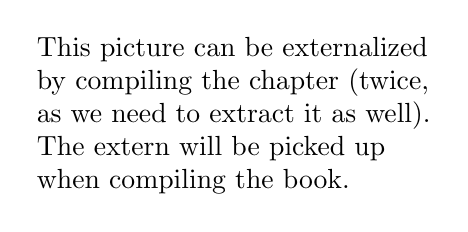
\begin{tikzpicture}
  \node[
    text width=5cm,
    align=flush left,
  ]
  {This picture can be externalized
    by compiling the chapter (twice, 
    as we need to extract it as well).
    The extern will be picked up
    when compiling the book.};
\end{tikzpicture}

\end{document}

  \end{tcblisting}
  \begin{tcblisting}{example title, title=a chapter file, listing only}
\mmzset{~memo dir=../book~}
  \end{tcblisting}
\end{tcboxedraster}

\pagebreak % manual

Section~\ref{sec:tut:working-on-a-picture} presented some ideas on how to work
on a single picture.  Those ideas can be all easily applied to the multi-file
situation.  For example, you could use \refmmz{readonly} on the chapter that you're
working on (and that chapter only).  This way, the preview of the chapter will
not be tarnished by the extern pages, and if you periodically compile it
without \refmmz{readonly}, or compile the book (which does not have the \refmmz{readonly}
set), you will have a reasonably up-to-date set of externs.

\begin{tcboxedraster}[raster columns=2, raster valign=top]{blankest}
  \begin{tcblisting}{example title, title=the main file, listing only}
\mmzset{memo dir=chapters/book}
% ...
\documentclass{article}

\usepackage{memoize}
\mmzset{~memo dir=book~}

\usepackage{tikz}

\begin{document}

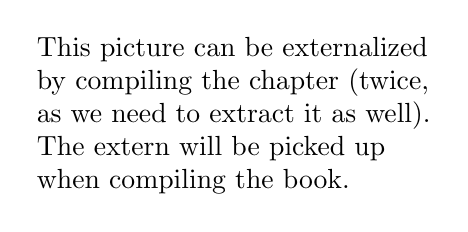
\begin{tikzpicture}
  \node[
    text width=5cm,
    align=flush left,
  ]
  {This picture can be externalized
    by compiling the chapter (twice, 
    as we need to extract it as well).
    The extern will be picked up
    when compiling the book.};
\end{tikzpicture}

\end{document}

  \end{tcblisting}
  \begin{tcblisting}{example title, title=the current chapter file, listing only}
\mmzset{memo dir=book, ~readonly~}
  \end{tcblisting}
\end{tcboxedraster}

\ExampleName{memoize.cfg._region_}
\makeexample{\examplename.tex.c1}
\begin{tcolorbox}[title=For \Emacs users]
  I often use this \refmmz{readonly} trick myself, but with a twist.  As an Emacs user,
  I don't use a \hologo{TeX}-based mechanism (such as the \pkg{docmute} package) to
  compile a chapter, but rely on the region compilation feature of Emacs'
  AUC\hologo{TeX} package.  AUC\hologo{TeX} offers a way to compile the current
  buffer (if you don't know what an Emacs buffer is, read ``file'') or region
  (roughly speaking, the selected text).  It does that by putting the buffer or
  the region into a file called |_region_.tex| while dressing it up in the
  preamble of the original document (when I'm working on a multi-file document,
  it correctly pulls the preamble from the main document).  This results in a
  compilable region file.  My trick is to detect whether I'm compiling a region
  (this is the job of |\ifregion|), and if so, put Memoize into the \refmmz{readonly}
  mode (an alternative trick would be to \refmmz{disable} it).

  This is the trick in a nutshell, but to make it really work we have to
  address one further issue: the original document and the region have to share
  memos and externs.  This happens automatically if the original document sets
  \refmmz{memo dir} explicitly (e.g.\ if a document called |doc.tex| contains
  \code{\refmmz{memo dir}=doc} in the preamble), but I'm lazy and don't want to
  write this in every document --- if I have to do that, what's the point of
  \refmmz{memo dir} I put into my \reffile{memoize.cfg} in
  section~\ref{sec:tut:memodir}?  Fortunately, the region file starts with
  |\message{ !name(|\meta{original document name}|.tex)}| to indicate the
  origin.  The complicated part of the code below (everything following
  \refcmd{mmzset}\braces{\refmmz{readonly}} parses this header to extract the
  \meta{original document name}, which is then fed to \refmmz{memo dir}.  Now,
  the trick works automatically for any document.\footnote{The assumption here
    is that \refmmz{memo dir} is in effect for the original document.  If not,
    the trick can be adapted to use \refmmz{prefix}.}

  \tcbinputexample{
    title=\tt memoize.cfg,
    attachment name=memoize-region.cfg,
    listing only,
  }
\end{tcolorbox}


\subsection{Writing a presentation?}
\label{sec:tut:beamer}

Memoize ships with built-in support for the most widespread \hologo{LaTeX}
presentation class, Beamer, in the sense that it can externalize a picture
which changes from overlay to overlay.  Before we learn how to use that
functionality, however, there's a peculiarity about loading Memoize in Beamer
to address.

\ExampleName{beamer}
\makeexample{\examplename.pdf}

\tcbinputexample{
  comment and listing,
  listing options app={lastline=2},
  warning, no attachment, title=,
  % 
  comment={Beamer opens the document PDF while loading the class, while
    Memoize requires the PDF from the previous compilation intact in order to
    extract the externs (when extraction is triggered internally, which is the
    default setting).  The solution is to load Memoize (a package) before
    Beamer (a class), which can be done by using \cs{RequirePackage} instead of
    the usual \cs{usepackage}. Easy, if hacky.},
  %
}

To memoize a piece of code which produces different results on different
overlays --- by virtue of containing |\pause|, |\only|, and\slash or related
commands --- apply key \Emph{\refmmz{per overlay}}.  Without this key,
externalization of the picture will end badly, with a single extern (the final
one) appearing on all overlays.  The key may be invoked either from a prior
\refcmd{mmznext} command,\footnote{Of course, \refmmz{per overlay} may also be
  invoked from \refcmd{mmzset}, but I guess this won't make sense often.  For
  example, if you set it for the entire presentation, and the presentation
  contains static memoized pictures as well, you will compile those pictures
  more times than necessary: once for each overlay, whereas once per frame
  would suffice.  It might occasionally make sense, however, to use \refmmz{per
    overlay} as an \refmmz{auto} option --- consult
  section~\ref{sec:tut:verbatim} to learn what that is.}  or executed in the
memoized code itself.  The example below illustrates the latter option, and
also shows that we may invoke it via its full path,
\refkeypath{/mmz}|/|\refmmz{per overlay}, when listed among options processed by
\pkg{pgfkeys}.\footnote{Read section~\ref{sec:per-overlay} to learn how the
  Beamer support is implemented.  The implementation only uses Memoize's public
  interface, so understanding it should help if you need to support some other
  presentation package.}

\tcbinputexample{
  listing options app={firstline=3},
  middle=1mm,
  comment={\def\dpwidth{0.27\linewidth}\def\epwidth{0.15\linewidth}%
    \raisebox{-\height}{\includeexamplepdf[extern page,left=0mm,right=0mm]{width=\epwidth,page=1,trim=1in 1in 0.4in 0.6in}}\hfill
    \raisebox{-\height}{\includeexamplepdf[document page,left=1mm,right=1mm]{page=2,width=\dpwidth}}\hfill
    \raisebox{-\height}{\includeexamplepdf[extern page,left=0mm,right=0mm]{width=\epwidth,page=3,trim=1in 1in 0.4in 0.6in}}\hfill
    \raisebox{-\height}{\includeexamplepdf[document page,left=1mm,right=1mm]{page=4,width=\dpwidth}}%
  },
}

\begin{tcolorbox}[warning]
  If the memoized code changes the value of Beamer's pause counter
  |beamerpauses|, e.g.\ by issuing a |\pause|, take care that (i) \refmmz{per
    overlay} is executed prior to any changes of |beamerpauses|, and that (ii)
  the final value of this counter in the memoized code is the same for all
  overlays.
\end{tcolorbox}


\subsection{When stuff sticks out}
\label{sec:tut:padding}

Some constructs --- like plain \hologo{TeX}'s \refcmd{llap} and \refcmd{rlap},
and, notably, \TikZ overlays --- fool \hologo{TeX} into thinking that the
``size'' of the typeset material is different than what it actually is.  This
can cause trouble for externalization: a piece of your picture might disappear!
In a sentence, the solution is to manually set the \emph{padding} of the
externs, but let's slow down a bit.

The \TikZ picture in the following example consists of node with a pin on the
right, but let's say we want to horizontally center this picture so that only
the node rather than the entire picture (including the pin) will be centered.
This can be achieved by adding key \refkey{/tikz/overlay} to the pin (actually,
we need to add it to both the pin and its edge).  \TikZ normally updates the
extents (called the bounding box) of the picture every time it puts something
in it; when \refkey{/tikz/overlay} is in effect, however, these updates are
temporarily disabled.  In effect, the \refkey{/tikz/overlay} key on the pin
below will fool \hologo{TeX} into thinking that the node is all there is to the
picture, so centering will work as desired.

\ExampleName{overlay}
\makeexample{\examplename.pdf N=4}
\tcbinputexample{
  after title pre={\ (no memoization)},
  comment={\centering
    % \includeexamplepdf[document page]{page=1,trim=1.8in 7.4in 1.8in 1.7in}
    \includeexamplepdf[document page]{page=1}
  },
}

What happens when we try to externalize this picture?  The example below shows
what would happen if Memoize had no concept of \emph{padding} --- which we
simulate by setting \code{\refmmz{padding}=0pt}.\footnote{Unlike in the rest of
  the manual, the extern pages in this section are shown without trimming the
  whitespace.}  Along with the rest of \hologo{TeX}, Memoize would be fooled
into thinking that the picture comprises of the node only, so the pin would
never make it into the extern.  You would end up with a document missing the
pin!\footnote{On the first compilation, the document page containing the figure
  without padding looks fine, as it uses the result of the compilation rather
  than the extern file.  But on the second compilation, when Memoize actually
  uses the extern, the pin disappears.}

\tcbinputexample[.tex][.c2]{
  after title pre={\ (memoization without padding)},
  attachment name=\examplename-no-padding.tex,
  sidebyside, lefthand ratio=0.3,
  comment={\centering
    \includeexamplepdf[size=minimal,boxrule=0.5mm,extern page,
      attach boxed title to top right={xshift=1.5mm,yshift=-1mm},
    ]{page=1}
  },
}


By default, Memoize puts an inch of space around (what it thinks is) the
externalized picture, and if the overlayed parts of the picture fit into this
inch of space, you will find them in the extern and therefore also in the
document.  In our example, however, the default padding is not enough --- the
pin is only partially visible.\footnote{You might wonder why I didn't make the
  default padding much bigger, like 10 inches.  \hologo{TeX} wouldn't be
  bothered (unless the resulting extern size exceeded its maximum dimension),
  but you might be, because with such a large default padding, all the externs
  would be huge, most often bigger than the document pages, and remember that
  the externs are first dumped into the document, where they can bother you.}

\tcbinputexample[.tex][.c3]{
  after title pre={\ (memoization with default padding)},
  attachment name=\examplename-default-padding.tex,
  listing and comment,
  middle=0.9mm,
  comment={\centering
    \includeexamplepdf[extern page,size=minimal,boxrule=0.5mm]{page=1}
  },
}

The solution is to set the padding manually.  Below, I used \refmmz{padding
  right} to only increase the padding on the right side (clearly, we also have
\refmmz{padding left}, \refmmz{padding top} and \refmmz{padding bottom}), but
if you're not bothered by a large extern, you can just use
\Emph{\refmmz{padding}}, which sets all four sides at once.  By the way, having
too much padding (almost) never hurts, and as you see, you can use (simple)
arithmetics in the value of these keys.

\tcbinputexample[.tex][.c4]{
  after title pre={\ (memoization with extra padding)},
  attachment name=\examplename-extra-padding.tex,
  listing and comment,
  middle=0.9mm,
  comment={\centering
    \includeexamplepdf[extern page,size=minimal,boxrule=0.5mm]{page=1}
  },
}

\enlargethispage{1ex} % manual
Incidentally, the \refmmz{padding} keys only change how
the externalized picture is \emph{stored}.  Memoize remembers the size of the
extern as seen by \hologo{TeX} (e.g.\ the bounding box of the picture as
reported by \TikZ, with overlayed parts of the picture protruding out of it),
and it uses that size when integrating the extern into the document --- so
everything works as it should!



\subsection{The verbatim mode}
\label{sec:tut:verbatim}

Not all code will peacefully submit to memoization.  In particular, this is the
case for environments which process the environment body verbatim (or perform
some other kind of \refcmd{catcode} magic).  A simple environment of this kind is the
standard \hologo{LaTeX} \refenv{verbatim}, but let us illustrate the issue with
\refenv{tcblisting}, which typesets a code listing alongside its compiled effect.
(This environment is defined by the |listings| library of package \pkg{tcolorbox}
and was used extensively during the production of this manual.)  To manually
memoize a \refenv{tcblisting} environment, we enclose it in a \refenv{memoize}
environment with a \Emph{\refmmz{verbatim}} key in the optional argument ---
without this key, the example below would produce nothing but
errors.\footnote{Memoize also offers a \emph{partial} verbatim mode, triggered
  by key \refmmz{verb}; in this mode, the braces retain their usual category
  codes.  Also note that the effect of \refmmz{verbatim} can be ``undone'' by
  key \refmmz{no verbatim}.}

\ExampleName{verbatim-manual}
\makeexample{\examplename.pdf}
\tcbinputexample{
  sidebyside,
  comment={\centering
    \includeexamplepdf[extern page]{page=1,trim=1in 1in 1in 1in}\\[1ex]
    \footnotesize
    (The document page is the same as for the \texttt{verbatim-auto} example below.)
  },
}

Using \refmmz{verbatim} from \refcmd{mmzset} or \refcmd{mmznext} works just as
well, and the latter can be very useful with automemoization, when some
environment (say, \env{tcolorbox}) generally does not require the verbatim mode,
but a specific occurrence does (say, because it contains some verbatim
construction such as \verb!|!\meta{verbatim text}\verb!|! of the \pkg{ltxdoc}
class).

However, for an environment such as |tcblisting|, it makes the most sense to
declare it verbatim in general, so that all instances of the environment will
be processed in the verbatim mode.  This is simple to do: add \refmmz{verbatim}
to the \refmmz{auto} keylist.

\ExampleName{verbatim-auto}
\makeexample{\examplename.pdf}
\tcbinputexample{
  sidebyside, % lefthand ratio=0.62,
  comment={\centering
    \footnotesize
    (The extern page is the same as for the \texttt{verbatim-manual} example above.)\\[1ex]
    \includeexamplepdf[document page]{page=2}\\
  },
}

In fact, you can add any \refkeypath{/mmz} key to the \refmmz{auto} keylist,
and the key will be applied to all occurrences of the command or the
environment.  For example, adding \refmmz{recompile} to the declaration of
|tcblisting| above would recompile all and only the |tcblisting| environments;
and as an \refmmz{auto} declaration only updates (rather than completely
replaces) a previous declaration, you can also say things like
\code{\refmmz{auto}=\refcmd{tikz}\braces{\refmmz{recompile}}} to recompile all
\TikZ pictures produced by the \cs{tikz} command (handy, as you don't know how
automemoization for \cs{tikz} was declared unless you've read
section~\ref{sec:tut:automemoization-details} or looked at the Memoize's source
code).


\subsection{The final version of your document}
\label{sec:tut:final}

Bluntly put, you might want to disable Memoize when compiling the final version
of your document, at least if you intend to distribute it in electronic form,
for two reasons:
\begin{itemize}
\item An externalized picture cannot contain hyperlinks.  Any hyperlinks (or
  hyperlink anchors) contained in the original picture will silently disappear
  during the production of the extern.
\item When the document contains many externs, the size of the resulting PDF
  can be several times the size of the PDF compiled without externalization.
\end{itemize}

Below, we list several ways of fully disabling Memoize.  You're of course
already familar with the first two ways, but what's this \refpkg{nomemoize}
package?  The rationale behind this package is that if you want to be
absolutely sure that there is no trace of memoization in your document (for
example, see the \refmmz{disable} -- \refmmz{enable} pitfall in
section~\ref{sec:tut:working-on-a-picture}), the best thing to do is to not
load the package at all.  However, you have all those \refcmd{mmzset}s etc.\ in
your source, so the document won't compile without
\cs{usepackage}\braces{\refpkg{memoize}}, right?  Right, but wrong.  Enter
\Emph{\refpkg{nomemoize}}, a dummy package which accepts all the commands that
Memoize does, but does nothing.  In effect, your document will compile, but you
can be sure that not a single memo or extern was loaded or produced.

\begin{tcbraster}[raster columns=3, raster force size=false, raster valign=top]
  \begin{tcblisting}{listing only, add to width=2.4em, enhanced}
\usepackage[~disable~]{memoize}
  \end{tcblisting}
  \begin{tcblisting}{listing only, add to width=-1.6em, enhanced}
\usepackage{memoize}
\mmzset{~disable~}
  \end{tcblisting}
  \begin{tcblisting}{listing only, add to width=-0.8em, enhanced}
\usepackage{~no~memoize}
  \end{tcblisting}
\end{tcbraster}

There is one issue you might need to resolve manually before package
\refpkg{nomemoize} works as intended, though.  If you have used any
\refkeypath{/mmz} keys outside \refcmd{mmzset}, you need to list them in
\refcmd{nommzkeys}.  For example, if you used \refmmz{per overlay} in the manner
illustrated in section~\ref{sec:tut:beamer}, i.e.\ as
\refkeypath{/mmz}|/|\refmmz{per overlay} among the \TikZ keys, you need to
write \refcmd{nommzkeys}\braces{\refmmz{per overlay}} into the document
preamble.

Another thing you might want to do once you have produced the final version of
the document (in fact, just before you disable Memoize for good) is clean up.
As we saw in sections~\ref{sec:tut:memodir} and~\ref{sec:tut:redefinitions},
Memoize produces a lot of auxiliary files (memos and externs) and it keeps the
old versions around!  Once your document is prepared, you can reduce the
clutter (and save some disk space) by deleting memos and externs belonging to
the work-in-progress versions of your document, and keep only those used in the
final version.

You could achieve this by deleting all the memos and externs (if you're using
the \refmmz{memo dir} directive, this amounts to the entire contents of the
memo directory) and compiling your document for the final couple of times.
However, there is an easier (but \hologo{TeX}-external) way: on the command
line, change into the directory containing your (main) document and write
\EmphTT{\refscript{memoize-clean.pl}} \meta{document name}\dmmz (substitute
|.py| for |.pl| to use Python rather than Perl). The script will inspect the
contents of the \dmmz record file to see which memos and externs were used in
the final compilation, and delete all other memos and externs belonging to the
given document.

\begin{tcolorbox}[warning]
  Deleting memos and externs is never an irreversible operation, as you can
  always recreate them, but it is still wise to be cautious when cleaning up.
  For one, avoid cleaning up after a compilation which produced errors; a
  failed compilation can lead to an incomplete \dmmz file, which can in turn
  lead to over-deletion.  Another bad idea is cleaning up after disabling
  Memoize for a part of a document, for the same reason.

  All that said, Memoize takes some precautions itself.  It will cowardly
  refuse to perform the clean-up when the \dmmz file is missing the
  end-of-file marker (|\endinput|), assuming that this indicates a fatal error
  in the previous compilation.  It will do the same in case the \dmmz file is
  absent or empty.  The latter is assumed to be a result of a globally
  \refmmz{disable}d memoization, but note that clean-up will be performed if
  memoization was disabled using package \refpkg{nomemoize}: that package does not
  touch the \dmmz file, so cleaning up should work as intended.
\end{tcolorbox}

As the final note, memos and externs (cleaned-up or not) may be copied (along
the document source) to another directory or machine, where they should be
picked up by Memoize.  There is no need to copy the \dmmz file (assuming that
the document PDF contains no extern pages waiting for extraction).


\section{Digging deeper}
\label{sec:potential-pitfalls}



\subsection{Good to know}
\label{sec:tut:good-to-know}


\paragraph{Line- and page-breaking} An extern can't be broken across lines or
pages.

Externalization of a chunk of code produces a PDF, which is included into the
document at subsequent compilations as a picture --- an unbreakable object (a
horizontal box) with fixed width and height.  Therefore, the original code
should produce an unbreakable object as well.  For example, this means that you
cannot externalize some text and expect \hologo{TeX} to break it across lines
or pages on subsequent compilations.  If you try, the compilation will succeed
--- without an error!  --- but your externalized text will end up in a single
line, as shown below.

\ExampleName{no-linebreaking}
\makeexample{\examplename.pdf N=2}
\tcbinputexample{
  bad,
  comment={\centering
    \includeexamplepdf[extern page,to be continued on right]
      {page=1,trim=1in 1in 14in 1in}\\[1ex]    
    \includeexamplepdf[document page]{page=2}\\[1ex]
    \includeexamplepdf[document page,title=the expected document page]
                      [\examplepath.c2.pdf]{page=1}
  },
}

That said, you \emph{can} externalize a paragraph or some other vertical mode
material using \refmmz{capture}|=|\refmmz{capture=vbox}, but beware that the
vertical spacing between the memoized material and its surroundings might
change.


\paragraph{\env{remember picture}}
\TikZ pictures using this key cannot be externalized.

Memoize will silently refuse to externalize any \TikZ picture using
\refkey{/tikz/remember picture} (see \PGFmanual{17.13}).  Such pictures
interact with the outside world --- they either reference or are referenced by
other pictures --- and are as such unsuitable for externalization.  For
example, while the colored boxes in this manual are generally externalized ---
out of principle \Smiley\ --- the title page illustration is not, and it cannot
be, because of the arrows connecting the various \TikZ pictures composing that
illustration.  Some packages use the \refkey{/tikz/remember picture} mechanism
under the hood, and are thus subject to this limitation; one example is package
\pkg{todonotes}, but in general, any package dealing with absolute positions on the
page will be limited in this way.

How does Memoize deal with this situation?  Well, by cowardly refusing to
externalize any code which uses \refkey{/tikz/remember picture} or a similar
mechanism for dealing with absolute positions.  Luckily, any such mechanism
eventually boils down to the \hologo{TeX} primitive \refcmd{savepos}, so
Memoize hacks --- or as we will say in this manual, \emph{advises} --- this
primitive to abort any ongoing memoization.  Initializing and then aborting the
memoization takes some time, to be sure, but the overhead is negligible,
especially in the light of the fact that \emph{not} aborting wreaks real havoc.

Memoize actually provides a user interface for aborting memoization.
Memoization can be aborted either manually, by executing \refcmd{mmzAbort}, or
automatically.  The latter is a generalization of the automemoization idea: a
command such as \refcmd{savepos} can be advised to abort memoization by
\refmmz{auto}|=|\refcmd{savepos}\bracestt{\refmmzauto{abort}}.  In Memoize,
commands take your advice seriously, so memoization will be aborted whenever
the advised command or environment is encountered.


\paragraph{Indirectly embedded environments} Such environments cannot be
memoized.

Read this if you got an error message such as |Environment "tikzpicture" ended
as "foo"|.

Some environments are defined so that they embed another environment using the
idiom shown on the left: the begin-code of the outer environment opens the
inner environment, and the end-code of the outer environment closes the inner
environment.  While this is a fine, and common, idiom, it messes up the
memoization of the inner environment. In the example on the right, trying to
\emph{auto}memoize a \env{minipage} environment (not recommended at all!) causes
trouble with package \pkg{sectionbox}.\footnote{This is a \texttt{Package
    collargs Error} because Memoize outsources the actual work of collecting
  the environment body to the auxiliary package CollArgs, described in
  section~\ref{sec:collargs}.}\fncomma\cprotect\footnote{Why does this happen?
  As mentioned in section~\ref{sec:tut:memodir}, Memoize keeps track of memos
  and externs by the MD5 sum of the memoized code.  But to compute that sum for
  an environment, Memoize has to \emph{grab} the environment body, meaning it
  has to collect the body in advance.  This presents no problem when
  \refcmd{end}\meta{environment name} is already present in the input stream at the
time \refcmd{begin}\meta{environment name} is executed, like when you use the
  environment normally in your document, or when some macro expands so that it
  produces both \cs{begin}\meta{environment name} and \cs{end}\meta{environment
    name} simultaneously --- so there would be no problem above if
  |\end{minipage}| occured in the beginning code of \env{sectionbox}.  The idiom
presented above is problematic for memoization because at the time \hologo{TeX}
executes |\begin{sectionbox}|, putting |\begin{minipage}| into the input
    stream, |\end{sectionbox}| is not yet executed and remains as it is.  The
  input stream therefore contains a pair of |\begin{minipage}| and
    |\end{sectionbox}|.  In the normal, non-memoizing course of events this
  would not be a problem, because |\end{sectionbox}| would eventually expand to
|\end{minipage}|.  During memoization, however, this \emph{is} a problem,
because, as we said, Memoize needs to grab the environment body: upon
encountering |\begin{minipage}|, it looks in the input stream for
  |\end{minipage}| --- but there is no |\end{minipage}| in the input stream,
there is only |\end{sectionbox}|, and this results in the |Environment
"minipage" ended as "sectionbox"| error.}

\begingroup
\ExampleName{sectionbox}
\makeexample{\examplename.tex.c1}
\mmzset{disable}
\begin{tcbraster}[raster equal height]
\begin{tcblisting}{listing only, bad, valign=center}
\newenvironment{foo}% ... args
{% the begin-code of foo
  % ...
  \begin{tikzpicture}
  % ...
}
{% the end-code of foo
  % ...
  \end{tikzpicture}
  % ...
}  
\end{tcblisting}
\tcbinputexample{
    bad,
    comment={\small\tt
      ! Package collargs Error: Environment\\"minipage" ended as "sectionbox".
    },
  }
\end{tcbraster}
\endgroup

What are your options in this kind of a situation?
\begin{enumerate}
\item The only way to perform any memoization here is to memoize the
  \emph{outer} environment --- if that makes sense.\footnote{This avoids the
    error because Memoize grabs and memoizes the outer environment, and while
    it is memoizing it, further memoization is switched off.}  You can do this
  either on a case-by-case basis, by enclosing it in the \refenv{memoize}
  environment, or automemoize it: \code{\refmmz{auto}=\marg{outer
      environment}\braces{\refmmzauto{memoize}}}.  
\item But what if memoizing the outer environment is out of the question?
  Then, the only way to avoid the error is to prevent the automemoization of
  the inner environment.
  \begin{enumerate}
  \item If you are facing a single occurrence of the problem, it is perhaps
    easiest to use key \refmmz{disable} just before the start of the outer
    environment.
  \item Otherwise, you can automatically disable memoization for the span of
    each occurrence of the outer environment: \code{\refmmz{auto}=\marg{outer
        environment}%
      \braces{\refmmzauto{nomemoize}}}.
  \item To deactivate the automemoization of the inner environment for the span
    of the outer environment, but otherwise allow for memoization inside the
    outer environment: \code{\refmmz{auto}=\marg{outer environment}%
      \braces{\refmmzauto{noop}, \refmmz{deactivate}=\meta{inner
          environment}}}. Key \refmmzauto{noop} does nothing but apply the
    given options (in this case, \refmmz{deactivate}=\meta{inner environment})
    to the advised command or environment.
  \end{enumerate}
\end{enumerate}

\subsection{Extraction methods and modes}
\label{sec:extraction}

Remember that in Memoize, externalization is a two-step process.  First,
externs are typeset on separate pages of the main document, called extern
pages.  Then, these extern pages are extracted out of the main document PDF
into extern files.  The process is illustrated on the title page.

Memoize is flexible in terms of which piece of software is used to perform
extern extraction.  It ships with three \emph{extraction methods}:

\begin{description}
\item[\refmmz{extract=perl}] A Perl script, \refscript{memoize-extract.pl}.
  This method is the default because it is fast and because Perl is usually
  already installed on a system running \hologo{TeX}.  However, you will most
  likely still need to install two pieces of software that the script depends
  on: Perl libraries \hreftt{https://metacpan.org/pod/PDF::API2}{PDF::API2} and
  the \hreftt{https://metacpan.org/pod/Path::Class}{Path::Class}, the
  installation guidelines can be found in section~\ref{sec:install}.
\item[\refmmz{extract=python}] A Python script, \refscript{memoize-extract.py}.
  This method is even faster than the Perl script, though not by much.  Try it
  out if you have problems installing Perl or the required libraries, or if the
  Perl script chokes on your document (see section~\ref{sec:troubleshooting}
  for the list of known issues).  Besides Python ($\geq 3.8$), you will also
  need the Python library \hreftt{https://pypi.org/project/pdfrw/}{pdfrw} or
  \hreftt{https://pypi.org/project/pdfrw2/}{pdfrw2}.  For the installation
  guidelines, see section~\ref{sec:install}.
\item[\refmmz{extract=tex}] \hologo{TeX}-based extraction requires no
  additional software, but it is much slower than the scripts.  As \hologo{TeX}
  can only produce a single PDF per compilation, an instance of \hologo{TeX}
  (loading the entire document PDF) has to be invoked for each extern, and this
  takes time (although the entire process is still much faster than the
  venerable \TikZ externalization library).
\end{description}

Memoize is also flexible in terms of how extern extraction is triggered,
providing two \emph{extraction modes}:

\begin{description}
\item[internal]\label{item:setup:who} By default, extern extraction is
  triggered internally, i.e.\ by Memoize during the compilation of the
  document; more precisely, any externs produced in a compilation are extracted
  during the next compilation.  To choose an extraction method other than the
  default Perl script, load Memoize with the package option
  \EmphTT{\refmmz{extract}=\meta{extraction method}}.

\item[external] Loading Memoize with with package option
  \EmphTT{\refmmz{extract}=\refmmz{extract=no}} instructs Memoize to \emph{not}
  trigger the (internal) extraction.  When instructed to use extraction
  ``method'' \refmmz{extract=no}, Memoize expects you to trigger the extraction
  yourself, in any way that is convenient to you: manually from the command
  line, or automatically through your editor, a Makefile, etc.  --- all Memoize
  cares about is that the extraction takes place before the next compilation of
  the document.
\end{description}

Summing up, the extraction mode and method are selected by providing the
appropriate value to package option key \refmmz{extract}; the possible values
are listed in the table below.  Note that this key can only be used as a
package option, or in \refcmd{mmzset} within \reffile{memoize.cfg}.  In
particular, it is disabled in the document preamble, because Memoize performs
extraction while it is loaded.

\medskip
\begin{center}
  \begin{tabular}{lll}
    \toprule
    extraction method&external program&Memoize invocation\\
    \midrule
    \refmmz{extract=perl}&\refscript{memoize-extract.pl}&\refcmd{usepackage}\braces{\refpkg{memoize}}\footnotemark\\
    \refmmz{extract=python}&\refscript{memoize-extract.py}&\refcmd{usepackage}\bracketstt{\refmmz{extract}=\refmmz{extract=python}}\braces{\refpkg{memoize}}\\
    \refmmz{extract=tex}&|pdftex|&\refcmd{usepackage}\bracketstt{\refmmz{extract}=\refmmz{extract=tex}}\braces{\refpkg{memoize}}\\
    \refmmz{extract=no}&none (external extraction)&\refcmd{usepackage}\bracketstt{\refmmz{extract}=\refmmz{extract=no}}\braces{\refpkg{memoize}}\\
    \bottomrule
  \end{tabular}%
  \footnotetext{Or
    \refcmd{usepackage}\bracketstt{\refmmz{extract}=\refmmz{extract=perl}}%
    \braces{\refpkg{memoize}}.  This is useful if you have changed the default
    using \reffile{memoize.cfg}.}%
\end{center}
\smallskip

For internal extraction, \hologo{TeX} must be allowed to execute the external
program implementing the chosen extraction method.  Both |memoize-extract|
scripts should be listed among restricted shell escape mode commands in your
\hologo{TeX} distribution; their execution should therefore be allowed under
the default, restricted shell escape mode.  However, the |pdftex| program,
executed by extraction method \refmmz{extract=tex}, is not listed there, nor
should it be.  If you are forced to use this fallback method, I suggest you
compile documents loading Memoize under the full shell escape mode, by adding
command-line option \docref{-shell-escape} (on \hologo{TeX}Live) or
\docref{--enable-write18} (on MiK\hologo{TeX}) to the invocation of the
\hologo{TeX} program.  The answers linked from question
``\href{https://tex.stackexchange.com/q/598818/16819}{How can I enable
  shell-escape?}''  on \href{https://tex.stackexchange.com}{\hologo{TeX}
  StackExchange} will tell you how you can ask your editor to do this for you.
  
You may use any extraction method to perform external extraction.  The simplest
option is to use the Perl or the Python script.  Supposing you are doing this
manually from the command line, change into the directory containing your
document, which should contain the auxiliary \dmmz file produced by Memoize,
and execute:
  
\begin{enumerate}[(a)]
\item \refscript{memoize-extract.pl} \meta{document name}\dmmz \hfill (for
  the Perl script)
\item \refscript{memoize-extract.py} \meta{document name}\dmmz \hfill (for
  the Python script)
\end{enumerate}

See sections~\ref{sec:.mmz} and \ref{sec:ref:extraction-perl-python} for
further details on the \dmmz file and the extraction scripts.

Things are a bit more complicated if you want to use the \hologo{TeX}-based
extraction method externally, because an instance of |pdftex| needs to be
invoked for each extern (and these have unwieldy names and can be many in
number), but Memoize can help you here by producing a shell script or a
makefile, executing which will extract all the externs at once. To have Memoize
produce a shell script, use package option
\code{\refmmz{record}=\refmmz{record=sh}} (or
\code{\refmmz{record}=\refmmz{record=bat}} on Windows); package option
\code{\refmmz{record}=\refmmz{record=makefile}} will make a makefile.  By
default, these files are named |memoize-extract.|\meta{document name} plus the
|.sh|, |.bat| or |.makefile| suffix.  If neither a shell script nor a makefile
works for you, you can also define your own kind of \emph{record file}, to be
processed by the external tool of your choice (and implementation) in order to
extract the externs; see section~\ref{sec:new-record-file} to learn how to do
this.


\subsection{From cross-references to the context}
\label{sec:cross-referencing}

Cross-referencing presents a challenge to externalization, because without
special provisions, the ``communication channel'' between the \cs{label} and the
\cs{ref} is broken once we start utilizing the extern.

One direction of the issue occurs when a \refcmd{label} within the memoized
code is referenced by a \cs{ref} on the outside.  Without the (built-in)
workaround, the \cs{label} command would only be executed when the extern is
being produced, but not on subsequent compilations of the document, when it is
merely included.  Memoize addresses this problem by generalizing
externalization (which can only produce a picture, the extern) to memoization
(which can additionally produce arbitrary code).  When Memoize is externalizing
code which contains a \cs{label}, it automatically replicates it into the
\emph{memo}, which is input into the document on subsequent compilations. In
effect, the memo--extern team will continue to produce the label even when it
is utilized rather than compiled.  As far as the author is concerned, \cs{label}s
in memoized code ``just work,'' without any observable differences to the
situation without memoization.  This is why we will not discuss this direction
of the issue here; a reader interested in how precisely the system works is
invited to read section~\ref{sec:memos}.

The other direction of the issue occurs when a \refcmd{ref} within the memoized
code references \cs{label} on the outside.  In this situation, the extern
should be recompiled when the value of the label it refers to changes.  Again,
Memoize addresses this problem in full generality, by associating with each
extern a \emph{context}, and recompiling the extern whenever the value of the
context changes.\footnote{The dependency of an extern upon prior definitions
  and such can also be addressed in a more \emph{ad hoc} manner, by recompiling
  manually; we have already touched upon this subject in
  section~\ref{sec:tut:working-on-a-picture}, and will revisit it in
  section~\ref{sec:tut:redefinitions}.}  All that needs to be done for \cs{ref}
and friends, specifically, is to advise them to add their reference keys to the
context.

As we shall see presently, for the author, the only difference between a
non-memoized and a memoized \cs{ref} is that the latter will take one more
compilation cycle to ``stabilize'' the resulting document.  (More precisely,
the memoized situation will take one more cycle if the reference is undefined
on the first compilation.)  Then, we will show how we can teach Memoize about
cross-referencing commands other than \cs{ref} and \cs{pageref}.  Finally, we will
learn about key \refmmz{context}, the backbone of the cross-referencing support
in Memoize.  (The inner workings of the context are further explained in
section~\ref{sec:c-memos}.)

\ExampleName{ref}
\makeexample{\examplename.pdf N=7}

When the memoized code contains a \cs{ref} referring to a label given in another
part of the document, the code is recompiled when (and only when) the reference
changes.  Let us look at the following example, jumping in at the point where
it was already compiled enough times that the resulting PDF had stabilized into
a single (document) page with correct references.  (Environment
\refenv{nomemoize} disables memoization
of \href{https://ctan.org/pkg/tikzlings}{Ti\emph{k}Zlings}, so that their
externs don't disturb us, and we can focus on the \cs{tikz} command, which does
get externalized and contains a \cs{ref}.)

\tcbinputexample[.tex][.c3]{
  after title pre={\ (with stable output after three compilations)},
  middle=1mm,
  comment={\centering
    \includeexamplepdf[document page]{page=1}
  }
}

Let us add an owl in front of the penguin.  In the next compilation, neither
the ``normal'' nor the memoized reference is yet updated, as expected --- in
this compilation, the new value of the penguin label only makes it into the
|.aux| file.

\tcbinputexample[.tex][.c4]{
  after title pre={\ (after the first compilation with the added owl)},
  no attachment,
  comment={\centering
    \includeexamplepdf[document page]{page=1}
  }
}

During the following compilation, the \refcmd{ref}s pick up the new value of the
penguin label, and the \cs{ref} inside the automemoized \cs{tikz} command
forces recompilation of the extern (\emph{how} this is done will be explained
later).

\tcbinputexample[.tex][.c5]{
  after title pre={\ (after the second compilation with the added owl)},
  comment only, no attachment,
  comment={\centering
    \includeexamplepdf[extern page]{page=1,trim=1in 1in 1in 1in}\quad
    \includeexamplepdf[document page]{page=2}
  }
}

In the next compilation, the resulting PDF is finally stabilized, as the
updated extern is (extracted and) included into the document.  

\tcbinputexample[.tex][.c6]{
  after title pre={\ (after the third compilation with the added owl)},
  comment only, no attachment,
  comment={\centering
    \includeexamplepdf[document page]{page=1}
  }
}

The message to take home?  When some memoized code contains a reference and
that reference changes, it will take three compilation cycles (so, one more
cycle than without memoization) for the resulting document to ``stabilize.''

Out of the box, Memoize supports the standard \hologo{LaTeX} cross-referencing
commands \cs{ref} and \refcmd{pageref}.  To automatically recompile code
containing some other cross-referencing command, like \refcmd{vref} of package
\pkg{varioref}, we use the advising framework implemented by package Advice.
This framework is a generalization of automemoization: we use the familiar
\refmmz{auto}, but with advice offered by \Emph{\refmmzauto{ref}} rather than
\refmmzauto{memoize}.

{\ExampleName{vref}
\makeexample{\examplename.tex.c1}
\tcbinputexample{listing only}}

Key \refmmzauto{ref} only works for commands which operate on a single
reference key.  However, that single key (which must be enclosed in braces) may
be preceded by optional argumen(s) of any kind.  Extensions to \refcmd{ref},
e.g.\ the \pkg{hyperref}'s variant, which accepts an optional |*|, work out of
the box.  Furthermore, Memoize offers support for cross-referencing commands
which work on multireferences and reference ranges, such as \pkg{cleveref}'s
\refcmd{cref} and \refcmd{crefrange}.  Those commands should be advised by
\refmmz{auto} keys \refmmzauto{multiref} and \refmmzauto{refrange},
respectively.

We have jumped into first example of this section with the assumption that it
had already been compiled several times, allowing the resulting PDF to
stabilize.  Let us now take a look at what happens at the very first, fresh
compilation of our original example (the one without the owl).  (Removing the
|.aux| file before compiling the example again will start afresh.)  The curious
thing is that we don't get the extern page containing
\tikz[baseline]\node[draw=red,thick,fill=yellow,anchor=base,font=\bf]{??};.
This is so because by default, Memoize aborts a memoization containing an
undefined reference.

\tcbinputexample[.tex][.c1]{
  after title pre={\ (after the fresh compilation of the original example)},
  comment only, no attachment,
  comment={\centering
    \includeexamplepdf[document page]{page=2}
  }
}

Now sometimes you might want to produce an extern even if it contains an
undefined reference --- for example, you might intend to write the code
containing the \cs{label} much later but enjoy the speed-up offered by Memoize
until then.  In that case, apply the \refmmz{auto} key \Emph{\refmmzauto{force
    ref}} to \cs{ref}.

\tcbinputexample[.tex][.c7]{
  after title pre={\ (after the fresh compilation with \refmmzauto{force ref})},
  attachment name=\examplename-force.tex,
  comment={\centering
    \includeexamplepdf[extern page][\examplepath.c1.pdf]{page=1,trim=1in 1in 1in 1in}\quad
    \includeexamplepdf[document page][\examplepath.c1.pdf]{page=2}
  }
}

However, note that when you use \refmmzauto{force ref}, \hologo{LaTeX} will
\emph{not} complain about the undefined reference once the extern containing it
is included (unless that reference also occurs in some non-memoized piece of
code).  Using \refmmzauto{force ref} is therefore a tiny bit dangerous, and
this is why \refmmzauto{ref}, with the abortion mechanism, is the default
handler for \cs{ref} and \refcmd{pageref}.

As already noted in the previous section, \refcmd{ref} works by appending the
cross-reference to the \emph{context}, the change of which triggers
recompilation.  Memoize initializes the context to contain the four
\refmmz{padding}s --- as a result, an extern recompiles if we change the
padding --- but we can append stuff to the context by ourselves, as well.
Below, we use key \Emph{\refmmz{context}} to append the font size (we'll talk
about the value given to this key a bit later); as a result, the picture is
recompiled whenever the font size changes.  Below, we change the font size
using command |\small|; changing the default size with a class option such as
|12pt| works as well.

\ExampleName{fontsize}
\makeexample{\examplename.pdf N=2}
\tcbinputexample{
  sidebyside, lefthand ratio=0.7, after title pre={\ (the first version)},
  comment={
    \includeexamplepdf[extern page]{page=1,trim=1in 1in 1in 1in}
  }
}

\tcbinputexample[.tex][.c2]{
  sidebyside, lefthand ratio=0.7, after title pre={\ (the second version)},
  no attachment,
  comment={
    \includeexamplepdf[extern page]{page=1,trim=1in 1in 1in 1in}
  }
}

How does this work? Key \refmmz{context} appends the given tokens to the
\emph{context expression}.  When creating an extern or trying to use it,
Memoize (fully) expands this expression and computes the MD5 sum of the
expansion.  This \emph{context MD5 sum} then serves as a part of the extern's
filename (see sections~\ref{sec:tut:memodir} and~\ref{sec:memos}).  In effect,
Memoize will only find (and utilize) the extern if \emph{the context MD5 sum
  computed during (attempted) utilization matches the one computed during
  memoization}.  

As revealed by looking at the \hologo{LaTeX} source code, \hologo{LaTeX} holds
the current font size in macro |\f@size|, and above, we have effectively added
the contents of this macro to the context.  Now, why didn't we simply write
\refmmz{context}|=\f@size|?  First, we used |\csname ... \endcsname| because we
were under the normal \hologo{LaTeX} catcode regime, where |@| cannot be a part
of the command name.  Of course, we could have temporarily changed the catcode
of |@| using |\makeatletter| and |\makeatother|, but I would advise against
that, because the approach does not work in general: it fails when key
\refmmz{context} is used \emph{within} memoized code (we will explain why in
section~\ref{sec:memos}).  Another reason why I recommend the |\csname
... \endcsname| approach is that it does not result in an error when the
control sequence is not defined (|\csname ... \endcsname| will expand to
|\relax| then); this behaviour is handy for undefined cross-references, for
example.  Second, why did I write |fsize={...}| around the control sequence?
Well, because I'm being paranoid, really.  Writing \refmmz{context}|={\csname
  f@size\endcsname}| would work just as well, but I like to explicitly
``announce'' the value to prevent any possibility of a conflict with an
alternative context.  Imagine that we don't use the ``announcements'' and we
decide to add some other dimension instead of the font size to the context.
Now if that dimension happened to have the same value as the font size, Memoize
would incorrectly pick up the ``font size extern'' instead of producing a new
one.

It bears emphasizing that whatever you add to the context expression must be
fully expandable, and also not merely declared as robust.  So writing
\code{\refmmz{context}=\cs{ref}\marg{key}}, for example, would be unwise, since
it would not work as intended when package \pkg{hyperref} is loaded.  (This
package declares \refcmd{ref} as robust, so it won't expand to the
cross-reference value.)  You have to look up where the cross-references are
stored internally; the cross-reference for \meta{key} turns out to be stored in
the internal control sequence |\r@|\meta{key}, so it is |\csname
r@|\meta{key}|\endcsname| that the \refmmzauto{ref} handler actually appends to
the context.

The padding and font-size contexts are useful quite generally.  However, the
context can be pretty command-specific, as well.  Consider the \pkg{skak}
package used for typesetting chess games.  The board is drawn using command
|\showboard|, but this command has no arguments, because it draws the state of
the board that is reached by the moves given by command |\mainline|.  Memoizing
|\showboard| as such will therefore yield the wrong result --- all the boards
will be one and the same board!  The solution is to provide the correct
context: we dig into the \pkg{skak} sources and realize that the current
board is stored in macro |\csname chessgame.skak.mainline\endcsname|.

\ExampleName{skak}
\makeexample{\examplename.pdf}
\tcbinputexample{
  sidebyside, lefthand ratio=0.48,
  comment={
    \includeexamplepdf[extern page]{page=1,trim=1in 1in 1in 1in,scale=0.45}\quad
    \includeexamplepdf[extern page]{page=2,trim=1in 1in 1in 1in,scale=0.45}
  }
}

If you remove \code{\refmmz{context}=\bracestt{...}} from the code above, you
will end up with a document where the final board drawn takes place of all the
boards.  This is so because in that case, all externs are written into the same
file, so the final extern overwrites the previous ones, but note that you will
only observe this after the second compilation, when the externs are actually
used.



\subsection{More on redefinitions and stale externs}
\label{sec:tut:redefinitions}

In this subsection, we elaborate on an issue touched upon at the beginning of
section~\ref{sec:tut:working-on-a-picture}: what happens if the memoized code
depends on some macro or style which gets redefined?  The answer was
``nothing,'' and one solution was to \refmmz{recompile} the code.  Let us take
the example from that section a bit further.  We will propose no new solution
or workaround, but deepen our understanding of the issue.

\ExampleName{redefinitions}
\makeexample{\examplename.pdf N=6}
\tcbset{
  recompile step/.style={
    sidebyside, lefthand ratio=0.74, title=,
    comment={\includeexamplepdf[blankest][\examplepath.c\theenumi.pdf]{#1}},
    /utils/exec={\addtocounter{enumi}{1}},
    enhanced, overlay app={\node[at=(frame.north west), font=\scriptsize, circle, fill=black!80!white, text=white, inner sep=1pt]{\theenumi};},
  },
}
\begin{tcboxedraster}[raster columns=1]{%
    title=Working on \texttt{\examplename.tex}, enhanced, breakable}
  \setcounter{enumi}{0}%
  \tcbox[blankest]{I like red. My emphasized nodes will have red background.}
  \tcbinputexample[.tex][.c1]{recompile step={page=2}}
  \tcbox[blankest]{Hmm, this particular node is really important,
    let me put the text in italics as well!}
  \tcbinputexample[.tex][.c2]{recompile step={page=2}, no attachment}
  \tcbox[blankest]{You know what? Perhaps yellow background would work better
    --- in general.}
  \tcbinputexample[.tex][.c3]{recompile step={page=1}, bad, no attachment}
  \tcbox[blankest]{How come my node is still red?!  Oh yes, I changed the
    style, so I have to recompile the extern!}
  \tcbinputexample[.tex][.c4]{recompile step={page=2}, no attachment}
  \tcbox[blankest]{Ahh, yellow background, that's much better.  But you know
    what, this double emphasis won't do after all, let me go back to the
    upright shape.}
  \tcbinputexample[.tex][.c5]{recompile step={page=1}, bad, no attachment}
  \tcbox[blankest]{Red???!???!? Ok, I know that recompiling will help, but what
    happened here?}
  \tcbinputexample[.tex][.c6]{recompile step={page=2}, no attachment}
\end{tcboxedraster}

What happened is that the externs from steps~1 and~5 share the very same code.
In step~1, this code was compiled when the red |emph| style was in effect, and
that extern lingered and was eventually picked up again in step~5, Memoize
having no idea that it is including an extern produced with the obsolete
definition of the style.

There are two points to this story.  First (and forgetting for a moment about
the context, which we started discussing in
section~\ref{sec:cross-referencing}), Memoize identifies externs (and memos) by
the code that produced them --- or more precisely, by the MD5 sum of the code,
as each piece of code has a unique (well, unique enough) MD5 sum.  Each extern
is saved in a file whose name contains this MD5 sum; see
section~\ref{sec:tut:memodir} for illustration.  Generally, this is a very
useful feature.  You can move your picture to another location in the document,
insert some other (externalized) picture in front of it, and so on, all without
triggering recompilation of the extern(s).  (None of this is possible with
\TikZ's externalization library, which identifies the externs by the order in
which they appear in the document.)

The downside of the MD5 sum approach is the potential pitfall illustrated
above, and the downside comes about because of the second point of the story:
Memoize does not attempt to delete the ``old'' externs.  (However, as described
in section~\ref{sec:tut:memodir}, stale memos and externs can be easily removed
using the \refscript{memoize-clean.pl} script.) That would be not only
dangerous (as any deletion inherently is) but also potentially wasteful: what
if you have only temporarily removed some code, or compiled only a portion of
the document --- you surely wouldn't want your hard-won externs to disappear in
such a situation!

The pitfall described above applies to any command which depends on parameters
which can be set prior to the invocation of the command, like \TikZ pictures,
which depend on the settings given in \cs{tikzset}.  After customizing the
settings, you will have to recompile the externs:
\refcmd{mmznext}\braces{\refmmz{recompile}} is useful when you only have to
recompile a single extern; use \refcmd{mmzset}\braces{\refmmz{recompile}}, or
the package option \refmmz{recompile}, to recompile all externs in the
document; and there is also the middle road: if you have changed only Forest's
settings, you can write
\code{\refmmz{auto}=\braces{forest}\braces{\refmmz{recompile}}} to recompile
all and only the Forest trees.

Above, we have seen the ``same code, same extern'' issue manifested ``through
time,'' i.e.\ Memoize was (incorrectly) reusing externs produced in previous
compilations, but the issue can also manifest ``through space.''  This can
happen if the same code appears twice in the same document --- but, crucially,
with some parameters which it depends on changed from one occurrence to the
next.  Observe what happens in the following example, where the settings for
|\progressbar| are changed by |\progressbarchange|.  After the first
compilation, everything looks fine.  But as both extern pages were produced by
the same code, they will be stored into the same file, the second one
overwriting the first one.  The second compilation pulls in the externs --- or
rather, the single extern --- resulting in the document containing the second
progressbar in the place of the first one as well.

\ExampleName{progressbar}
\makeexample{\examplename.pdf N=2}
\tcbinputexample{
  bad, float,
  comment={
    \begin{tcbitemize}[raster columns=3,raster equal height,halign=center,valign=center]
      \tcbitem[title=After 1\textsuperscript{st} compilation]
      \includeexamplepdf[extern page,remember as=extern1]{page=1,trim=1in 1in 1in 1in}\\
      \includeexamplepdf[extern page,remember as=extern2]{page=2,trim=1in 1in 1in 1in}\\
      \includeexamplepdf[document page]{page=3}
      \tcbitem[title=After extern extraction\vphantom{p\textsuperscript{nd}}]
      \includeexamplepdf[my boxed title=the extern file,attach shifted boxed title to top right,remember as=externfile]{page=2,trim=1in 1in 1in 1in}
      \tcbitem[title=After 2\textsuperscript{nd} compilation]
      \includeexamplepdf[document page,remember as=doc][\examplepath.c2.pdf]{page=1}
    \end{tcbitemize}
    \begin{tikzpicture}[remember picture,overlay]
      \draw[->, thick, red] (extern1.east) to[out=east, in=west] ([yshift=0.5ex]externfile.west);
      \draw[->, thick, red] (extern2.east) to[out=east, in=west] ([yshift=-0.5ex]externfile.west);
      \draw[->, thick, blue] (externfile.east) to[out=east, in=west] (doc.west);
    \end{tikzpicture}
  },
}

The same ``extern duplication'' can arise due to how a particular command is
implemented.  Say we deactivate automemoization of Forest trees
(\code{\refmmz{deactivate}=forest}), but keep on automemoizing \TikZ pictures.
Forest uses \refenv{tikzpicture}\noprint{\refenv{forest}} under the hood (a
lot); in particular, the tree itself is typeset as a \env{tikzpicture}
environment.  But the code that typesets it is the same for all trees,
regardless of their content (the actual content of the tree is hidden in
various macros and boxes, rather than ``pasted'' into the \env{tikzpicture}).
Consequently, the final tree of the document will overwrite all other trees in
the document, just as the second (and thus final) progress bar overwrote the
first one above.\footnote{That is assuming that \hologo{TeX} doesn't simply
  spew a bunch of errors. This can happen as well.  In the interest of full
  disclosure, compiling a Forest tree in the situation described above would
  actually also produce --- but only in the first compilation --- a number of
  small empty extern pages, one for each node of the tree.  A promise: Forest
  will soon fully support Memoize and (among other things) avoid this pitfall.
  But the principle will remain.}  Ouch!

Generally speaking, this final sort of extern duplication issue can arise
whenever we have an ``outer'' command that we don't want to (auto)memoize which
uses an ``inner'' command that we \emph{do} want to automemoize.  The solution
is to use the \refmmz{auto} key \refmmzauto{nomemoize} on the outer command;
remember that this key disables memoization for the space of the command or
environment.  For example, the correct way to ``deactivate'' automemoization of
\env{forest} environments (but keep automemoizing \TikZ pictures) is
\code{\refmmz{auto}=\bracestt{forest}\braces{\refmmzauto{nomemoize}}}.




\subsection{Supporting Memoize in your package}
\label{sec:tut:package}

\subsubsection{Loading Memoize?}
\label{sec:loading-memoize}

So you want to support Memoize in your package? That's great!

What form precisely this support will take of course depends on your package.
For some commands, a simple \refmmz{auto} declaration will suffice; for other
commands, you might need to write a dedicated \emph{memoization driver}, as
explained in section~\ref{sec:memoization-drivers}.  However, one thing is
clear: you \emph{don't} want to require Memoize's presence by
\cs{RequirePackage}\braces{\refpkg{memoize}} in your package.  That would
trigger memoization, but triggering memoization should be left at the sole
discretion of the author.  The question is, if you're not allowed to load
Memoize, how can you even issue the \refmmz{auto} declaration?

Well, it's not that you really want to \emph{memoize} anything; you want to
make the commands of your package \emph{memoizable}.  So:
\cs{RequirePackage}\braces{\Emph{\refpkg{memoizable}}} --- and note that in
`memoizable', the final `e' of `memoize' is dropped, apparently this is the
correct way to spell it.

Loading \refpkg{memoizable} does nothing if Memoize is already loaded, and
behaves like package \refpkg{nomemoize} otherwise --- remember from
section~\ref{sec:tut:final} that \refpkg{nomemoize} is a dummy package which
accepts all the commands that Memoize does, but does nothing.

I have decided to require that Memoize must be loaded before any package that
supports it.  Allowing for an arbitrary loading order would complicate the
implementation (and possibly even turn out to be problematic), and furthermore,
Memoize likes to be loaded early anyaway, because it needs to be loaded before
the document PDF is opened if it is to perform the embedded extern extraction.
I don't think the ordering requirement will cause any problems --- let me know
if it does!  --- but perhaps it is wise to inform the author about it in the
documentation of your package (I did so at the end of
section~\ref{sec:tut:automemoization}).  Anyway, I have enforced the
requirement by raising an error and refusing to load the package in case
Memoize detects \refpkg{memoizable} to be loaded.

Note that the loading order requirement implies that you can use
|\@ifpackageloaded{memoize}| to specifically react to the presence Memoize, if
necessary.


\subsubsection{Memoizable design}
\label{sec:memoizable-design}

Many commands and environments can be submitted to externalization with a
single-line \refmmz{auto} declaration, as illustrated in
section~\ref{sec:tut:automemoization}, perhaps requiring an addition to the
context (section~\ref{sec:cross-referencing}), or some pre- or post-memoization
code (section~\ref{sec:tut:beamer}).  In some situations, however, these simple
approaches won't work.  Most often, this will happen when the extern must be
integrated into the document in some special way.  For example, a command might
internally create floating material, or surround the core typeset material with
some stretchable space.\footnote{Commands and environments of package
  \pkg{tcolorbox} exhibit both these issues (see \pkg{tcolorbox} options |float|,
  |before| and |after|), and were in fact the inspiration for several technical
  details of Memoize.}  None of these behaviours can be replicated by merely
including the extern; with respect to the stretchable space, remember that an
extern, being a picture, has fixed size, so if our extra space ended up in the
extern, it would lose the stretchability.

The key to successful memoization of problematic commands is their design.  In
a nutshell, the idea is to \emph{break up the command's definition into two
  parts, the outer command and the inner command, and only submit the inner
  command to automemoization}.  We will illustrate this with a simple
environment --- |poormansbox| --- which produces a potentially framed box of
the given width, and surrounds this box with some configurable material --- by
default, this material will be stretchable vertical space, and this will be the
source of our memoization problem.  (In terms of user experience, the solution
in this section will leave something to be desired, but we will revisit the
example in section~\ref{sec:memoization-complex-single-driver} and make things
right.)

Let us first take a look at a document using our to-be-developed box
environment.  The |poormansbox| environment takes one optional argument, a
keylist of options, which can also be set with the |\pmbset| command.  This
being a \textbf{p}oor \textbf{m}an's \textbf{b}ox, it doesn't recognize many
options.  One can set the |width| of the box, or request that it occurs in a
|frame|, and the surrounding material can be configured using keys |before| and
|after|.  As we will see later in the listing of the package, the box is
|\linewidth| wide by default, has no frame, and is surrounded by vertical glue
|\vskip 2ex plus 1ex minus 1ex| (|2ex| of natural vertical space which may both
stretch and shrink for |1ex|); furthermore, the default value of |before|
contains |\centering| to center the box horizontally (centering is of course
only observable when we change the width of the box).

\ExampleName{poormansbox}
\makeexample{\examplename.sty}
\makeexample{\examplename.pdf}
\tcbinputexample{
  sidebyside, lefthand ratio=0.482,
  comment={\centering
    \includeexamplepdf[document page,left=0pt,right=0pt]
                      {page=1,scale=0.5,trim=0mm 3mm 0mm 3mm}
  },
}

You might want to play with the example to see that the surrounding vertical
space is indeed stretchable.  The example is set up so that the surrounding
space is shrunk a bit to fit all the material onto one page.  But if you remove
the final |\lipsum[144]|, the natural amount of all vertical space can be
accommodated on the page, so you should observe an increase of vertical
spacing.

You might have noticed that the example contains nested |poormansbox|es: the
second box (the one which contains |\lipsum[66]|) is nested within the first
one (between |\lipsum[101]| and |\lipsum[75]|).  This is intentional: when we
will revisit the |poormansbox| example in
section~\ref{sec:memoization-complex-single-driver}, the implementation will
have to pay special attention to nesting (which presents no problem to the
implementation in this section).

As you can see in the package listing below (\texttt{\examplename.sty}), the
implementation of our environment is straightforward.  We first define the
configuration command |\pmbset| and the option keys (we're using
\pkg{pgfkeys}), and set the option defaults.  Then, we move on to the
environment itself: we apply the given options, execute the pre-code, typeset
the box (which is a |minipage| of the given width, potentially wrapped in a
|\fbox|), and execute the post-code.

\tcbinputexample[.sty]{listing only, float}

\ExampleName{poormansbox-memoizable}
Now let's make our |poormansbox| externalizable (\texttt{\examplename.sty}).  As
announced above, the idea is to split the definition of the environment into
the outer part (below, the user-level environment |poormansbox|), which
(applies the options and) executes the pre- and the post-code, and the inner
part (below, the macro |\@poormansbox|), which typesets the actual box.  If we
then then submit |\@poormansbox|, rather than |poormansbox|, to
automemoization, the outer part will be executed at every compilation (giving
us stretchable space if we request it), while the inner command will be
executed (and memoized) at the first compilation, and substituted for the
extern (the fixed-size box) at subsequent compilations.\cprotect\footnote{You
  might have wondered why our definition of the |poormansbox| environment grabs
  the body into an argument (|+b|, yielding |#2|), necessitating the use of
  |\NewDocumentEnvironment| over the venerable |\newenvironment|.  One reason
  was that having the environment body as an argument simplifies wrapping the
  |\fbox| around the |minipage|, but there is a more important reason.  If we
  did not grab the environment body, we would have to implement the internal
  part of the definition as an environment (|@poormansbox|) as well, and embed
  it into the user-level environment using the following idiom:
  |\newenvironment{poormansbox}[2][]{...\begin{@poormansbox}}{\end{@poormansbox}...}|.
  However, as illustrated in section~\ref{sec:tut:good-to-know}, automemoizing
  an environment indirectly embedded in such a way produces an error, because
  Memoize is prevented from collecting the environment body.}

\makeexample{\examplename.sty}
\makeexample{\examplename.pdf}% just to know if it compiles fine
\tcbinputexample[.sty]{listing only, float}

Looking at the definition of the internal |\@poormansbox| command, it might
strike you as weird that we have equipped this command with an optional
argument (|#1|) it never uses.  However, this optional argument is crucial for
memoization.  It will become a part of the memoized code (note
\code{\refmmzauto{args}=om} in the \refmmz{auto} declaration) and thereby
ensure that Memoize will produce separate externs for invocations of
|\@poormansbox| with the same environment body but different options; or in
other words, it will ensure that changing the options recompiles the
extern.\cprotect\footnote{Of course, this only holds for options given in the
  optional arguments; if the user changes an option value using a prior
  \cs{pmbset} (and that option does not occur in the optional argument),
  Memoize won't detect the change.  But the end-user knows about this issue, as
  it was addressed in sections~\ref{sec:tut:working-on-a-picture}
  and~\ref{sec:tut:redefinitions}, and she is also aware of two workarounds:
  manual recompilation, or setting the context
  (section~\ref{sec:cross-referencing}).

  While we're on the subject of the context, note that it is also possible to
  deploy context to trigger recompilation of the inner command upon change of
  parameters it depends on.  We could simply omit the optional argument of
  \cs{@poormansbox} and add
  \refmmz{context}|={width=\pmb@width,frame=\ifpmb@frame true\else false\fi}|,
  to the \refmmz{auto} declaration.  The advantage of such an approach is that
  Memoize reacts to the change of parameters regardless of whether they are set
  using the optional argument or \cs{pmbset}.  However, the approach is
  unfeasible for commands depending on many parameters: can you imagine listing
  all the \TikZ options in the context?  Not to mention that a particular
  picture usually only depends on a small subset of these options --- by and
  large, \TikZ externs would get recompiled too often if the context contained
  all \TikZ options.}\footnote{I have toyed with the idea of
  splitting (using \pkg{pgfkeys} key filtering) the given options into outer
  options, relevant for the outer command, and inner options, relevant for the
  inner command, and only passing the inner options to the inner command.  The
  thought was that would (i) avoid recompiling the extern when only outer
  options change, as these options don't affect the inner command, and (ii)
  avoid applying the inner options when utilizing the extern, as these options
  don't affect the outer command.  However, it then hit me that the end-user
  might define a style which incorporated both inner and outer options --- I
  know I do this with my |tcolorbox|es.}

The downside to automemoizing an internal command is that this might be
counter-intuitive for the author.  For example, to deactivate automemoization
of |poormansbox|, the author will have to write
\refcmd{mmzset}\bracestt{\refmmz{deactivate}=\cs{@poormansbox}} (note the
|\@|), but they will have no clue they have to do this unless they have
carefully read |poormansbox|'s documentation.  Even worse, the above
\refcmd{mmzset} command will not work unless surrounded by |\makeatletter| and
|\makeatother|, as it refers to an internal control sequence containing |@|.
Well, Memoize offers \refmmz{auto csname}, \refmmz{activate csname} and
\refmmz{deactivate csname}, so that |@| catagory code manipulations can be
omitted by writing \refcmd{mmzset}\bracestt{\refmmz{deactivate
    csname}|=@poormansbox|}, but still.

Another downside could occur when you use the same (automemoized) internal
command in service of several user interface commands.  For the sake of
illustration, assume we have also defined an UI-macro |\pmb| which again relies
on |\@poormansbox|.  How is the author to deactivate automemoization of |\pmb|
but leave the |poormansbox| environment intact?  This is how:
\refcmd{mmzset}\bracestt{\refmmz{auto}=\cs{pmb}\bracestt{\refmmzauto{args}=m,
    \refmmzauto{nomemoize}}}.  Again, counter-intuitive; the author expects
\refcmd{mmzset}\bracestt{\refmmz{deactivate}=\cs{pmb}} to work.

One other consequence of this approach is that the code included in the c-memo
(if \refmmz{include source in cmemo} is in effect) will not faithfully reflect
the source: as shown in the c-memo listing below, it will contain
|\@poormansbox{...}| instead of |\begin{poormansbox}...\end{poormansbox}| ---
even if this might actually count as an advantage, as the discrepancy will at
least inform the author who refuses to read the fine material accompanying our
|poormansbox| that something funky is going on.

\begingroup
\relaxmmzcommands
\def\mmzNewCMemo#1{% fetch the last c-memo filename
  \def\mycmemo{#1}%
}
\input{\examplepath.mmz.c1}
\sed{%
  s/[]]\lbrace/]\n\space\space\space\space\space\space\space
           \space\space\space\space\space\space\space\lbrace/;
}{\exampledir\mycmemo}
\tcbinputlisting{
  listing only,
  listing file=\exampledir\mycmemo,
  example title,
  title=the c-memo of the last \texttt{poormansbox} environment,
  left=0.5em, right=0em,
}
\endgroup

In a nutshell, automemoizing an internal command might be counter-intuitive for
the author.  But the core idea --- to support memoization of a resistant
command by splitting its definition into the outer and the inner command --- is
sound, and we will elaborate on this idea in
section~\ref{sec:memoization-complex-single-driver}, where we will revisit our
|poormansbox| example and develop a variant of this environment which is both
memoizable and user-friendly.


\section{Under the hood}
\label{sec:under-the-hood}

This chapter is written for three audiences: a curious user who wants to
know how Memoize does what it does; a package writer who wants to support
Memoize in a tricky situation; and myself, lest I forget why I made the design
decisions that I made.

\subsection{The entry point}
\label{sec:Memoize}


From the author's perspective, the functionality of this package is entered
either through the manual memoization commands (macro \refcmd{mmz} and
environment \refenv{memoize}), or via automemoization.  And while that is
correct, those user interface entry points merely determine what code is
submitted to memoization, and set any options specific to the upcoming
memoization.  The real fun starts with command \Emph{\refcmd{Memoize}}, which
is eventually executed by both manual and automatic memoization.

Not every call to \refcmd{Memoize} results in memoization.  Calling this macro
has three possible outcomes.  It can result in \emph{memoization}, which
produces the memos and externs; in \emph{utilization} of the result of an
earlier memoization (which boils down to inputting the memos); or in
\emph{regular compilation}, whereby the code is compiled
(almost)\footnote{\label{fn:regular-compilation-almost}This is absolutely true
  for memoized code which is ``contained'' in the sense of not peeking into the
  input stream following the memoized code.  In general, code which fails to
  satisfy this containment requirement is most likely simply not memoizable;
  but there are borderline cases.  For example, \refcmd{ignorespaces} at the
  end of some code will have the expected effect in the absence of Memoize, but
  no effect when executed either during memoization or regular compilation
  under Memoize, simply because it will hit some code belonging to Memoize
  rather than the continuation of the document.  Memoize offers the
  \refmmz{ignore spaces} provision to work around this specific problem.} as if
Memoize was not there.  Which outcome obtains depends on several factors.  The
decision logic is depicted below, and note that you can \refmmz{trace} the
action on the terminal.

\begin{center}
  \begin{forest}
    yes/.style={edge=->,edge label={node[font=\scriptsize,pos=0.4,left,#1]{yes}}},
    no/.style={edge=->,edge label={node[font=\scriptsize,pos=0.4,right,#1]{no}}},
    use/.style={content=utilization\\(of the cc-memo)\vphantom{dj},fill=orange,align=center},
    memoize/.style={content=memoization\vphantom{dj},fill=green},
    compile/.style={content=regular compilation\vphantom{dj},fill=emphcolor},
    for tree={
      l sep*=1.5,
      if n children={0}{}{align=center},
      child anchor=north,
    },
    [Is Memoize enabled?\\(\refcmd{ifmemoize}),
      [Are we currently undergoing memoization?\\(\refcmd{ifmemoizing}), yes
        [,compile, yes]
        [Is the\\\refmmz{recompile}\\mode in effect?, no
          [,memoize, yes]
          [Do the relevant\\memos and externs exist?, no
            [,use, yes]
            [Is the\\\refmmz{readonly}\\mode in effect?,no
              [,compile, yes]
              [,memoize, no]
            ]
          ]
        ]
      ]
      [,compile, no]
    ]
  \end{forest}
\end{center}

As the memoization options were already set by the user interface entry points,
you might expect, quite reasonably, that \refcmd{Memoize} takes a single
argument, the code submitted to memoization.  After all, what more does it
need?  Clearly, executing this code is what produces the typeset material, and
to detect whether the code has ``changed'' (in order to recompile the memos and
externs), we compute the MD5 sum of this very code, don't we?  Well, the
reality is a bit more complicated.  When it comes to automemoized commands, the
code which the MD5 sum is computed off of (and which is displayed in the c-memo
if \refmmz{include source in cmemo} is in effect) is not exactly the same as
the code we compile (during either memoization or regular compilation).  We'll
see what the difference is in section~\ref{sec:tut:automemoization-details};
what matters here is that we must provide \refcmd{Memoize} with both and that
this macro therefore takes two arguments: the \emph{identification code}, which
the MD5 sum is computed off of, and the \emph{executable code}, which, well, is
the code that gets executed during memoization (or regular compilation).

Let's illustrate this with an example which is probably entirely useless (but
don't worry, we'll get to a realistic example in
section~\ref{sec:tut:automemoization-details}).  We first memoize some text
manually, using command \refcmd{mmz}, and then do something very stupid: we use
this very text as the identification code for the following \refcmd{Memoize},
even if the executable code of that command is completely different.  The
second line of the typeset output should convince you that the first argument
to that command was really used to produce the extern; and one further
compilation should convince you that the first argument was indeed used to
identify the extern: the extern produced by \refcmd{mmz} was overwritten by the
extern produced by \refcmd{Memoize}, in the fashion of the |progressbar|
example from section~\ref{sec:tut:redefinitions}.

\ExampleName{memoize-internal}
\makeexample{\examplename.pdf N=2}
\tcbinputexample{
  comment={%
    \includeexamplepdf[document page,
      after title pre={\ (after the first compilation)}
    ]{page=3}\hfill
    \includeexamplepdf[document page,
      after title pre={\ (after the second compilation)}
    ][\examplepath.c2.pdf]{page=1}
  },
}

The example above also illustrates a(nother) peculiar feature of
\refcmd{Memoize}.  \refcmd{Memoize} does not open a new \hologo{TeX} group, but
it \emph{expects a group to be opened prior to calling it}, as it will issue an
|\endgroup| at some point.  Specifically, the memoization group will be closed
before regular compilation or utilization, but after memoization.  If you want
to know why, read the boxed text below.

\begin{tcolorbox}[title=\string\Memoize\ and grouping, enhanced, breakable]
  One important desideratum behind the design of Memoize was that using the
  package should disrupt the original, Memoize-less compilation as little as
  possible.  In particular, if the memoized code contains local assignments
  whose effect (in the original compilation) persists into the rest of the
  document (until the end of the surrounding \hologo{TeX} group, of course),
  wouldn't one want these local effects to persist when Memoize is around, as
  well?  Fortunately, most memoized code does not have persistent local effects
  (at least for me, it is usually environments, like \env{tikzpicture}s, that I
  want to memoize, and environments introduce a group anyway) --- fortunately,
  because there are design reasons for enclosing memoization in a \hologo{TeX}
  group (or two), and this enclosure will of course cancel the effect of local
  assignments in the memoized code.

  For one, the user interface memoization commands, such as \refcmd{mmz} and
  automemoized commands, allow for options specific to a particular piece of
  memoized code (the options given as the optional argument to manual
  memoization, the next-options and the auto-options), and to delimit their
  effect, it makes most sense to apply them in a group.  I have toyed with the
  idea of working around the introduction of a group by manually saving and
  restoring all the options, but I quickly gave up on this line of thought.
  For one, manually saving and restoring the options would be cumbersome and
  error-prone, and probably also slower than using the group.  But even worse,
  all that work would not really solve the problem of the persistence of local
  effects, because memoization itself introduces a group, as well: during
  memoization, the typeset material is collected into a box, and opening a box
  introduces a group.  In some particular situations, this could be avoided by
  typesetting the memoized code as-is and collecting the resulting material
  using |\lastbox|, but this approach cannot work in general.  In general,
  memoization will take place in a group, so the issue of local effects must be
  addressed in some other way.  Memoize offers the following workaround: during
  memoization, the memoized code can (globally) add code to the \refmmz{after
    memoization} hook, which gets executed immediately after closing the
  memoization group.

  Does this mean it would be best if the user interface memoization commands
  straightforwardly surrounded \refcmd{Memoize} by |\begingroup| and
  |\endgroup|?  For example, \refcmd{mmz} would open the memoization group, let
  \refcmd{Memoize} do its work, and then close the group.  Not really.
  Remember that memoization is not the only possible outcome of calling
  \refcmd{Memoize}.  Perhaps we can at least retain the local effects of a
  regular compilation, and of utilization?

  We can, by finely tuning the timing of the memoization group closure within
  \refcmd{Memoize}.  This command is designed to close the memoization group
  after memoization, but before regular compilation and utilization.  Closing
  the group after memoization makes sure that the given options are in effect
  during this process.  By closing the group prior to regular compilation,
  regular compilation of the memoized code (which takes place when Memoize is
  disabled, for example) is guaranteed to have (almost, see
  footnote~\ref{fn:regular-compilation-almost}) exactly the same effect as the
  compilation of that code in absence of Memoize; in particular, the effect of
  any local assignments will persist into the rest of the document.  Finally,
  closing the group before utilization simplifies the construction of the memo
  in the cases where we need to replicate local effects of the memoized code
  --- the group closed, there is no need to smuggle local assignments out of a
  memo.
\end{tcolorbox}

\subsection{Memos}
\label{sec:memos}

Up until now, we have pretended that there is a single kind of a memo file.  In
truth, there's two kinds: \emph{code memos}, or \emph{c-memos} for short; and
\emph{code--context memos}, or \emph{cc-memos} for short.  In this section, we
will learn what they are for, and how they look like --- and also a bit on how
they are produced, even if the details on that will have to wait until
section~\ref{sec:memoization-drivers}.

We will see that when Memoize utilizes memos, c-memos are processed first.  But
conceptually, cc-memos are more important, so we will start the discussion with
these.

\subsubsection{Cc-memos (and extern inclusion)}
\label{sec:cc-memos}

When it is input, a cc-memo replicates the effect of the memoized code.  This
includes the reproduction of its visual output, which takes the form of
inclusion of any externs produced by memoization.  And yes, you got the
implication right: a cc-memo can have any number of associated externs,
including zero, even if the most common case is that of exactly one extern per
cc-memo.  The number of externs mostly depends on the memoization driver (see
section~\ref{sec:memoization-drivers}); the default driver always produces
exactly one extern.

A cc-memo is located in the \refmmz{prefix directory} determined by key
\refmmz{prefix} (everything up to the final |/| in the value of this key, or
the current directory if this value contains no |/|).  You can recognize it by
its filename, which has the following form (\meta{prefix name} is everything
following the final |/| in the value of \refmmz{prefix}):
\begin{center}
  \code{\meta{prefix name}\meta{code md5sum}-\meta{context md5sum}.memo}
\end{center}

In fact, this is how Memoize recognizes --- or rather, searches for --- a
cc-memo as well: Memoize will utilize a cc-memo when the code and the context
MD5 sum computed during an attempted utilization match the code and the context
MD5 sum computed during some previous memoization (for details on the context
MD5 sum, see section~\ref{sec:c-memos}).  In detail, a cc-memo is created at
the end of memoization, at which point Memoize computes the MD5 sum of the
memoized code and the MD5 sum of the context, and writes the results of
memoization into the cc-memo identified by (the prefix and) these two MD5 sums.
And when Memoize, on a subsequent compilation, encounters a piece of memoized
code, it again computes the MD5 sum of that code and the MD5 sum of the
context, and tries to input the cc-memo identified by (the prefix and) these
two MD5 sums.  If the inputting is successful, we have utilized the cc-memo
(which in the typical case amounts to including the one associated extern); if
the cc-memo cannot be found, Memoize starts the memoization process, which
creates the memos and the externs.

Let us take a look at the contents of a cc-memo in detail.  Here's a typical
cc-memo (it belongs to the titlepage penguin):

\begingroup
\relaxmmzcommands
\def\mmzNewCCMemo#1{% fetch the first cc-memo filename
  \def\myccmemo{#1}%
  \endinput
}
\input{\exampledir titlepage.mmz.c1}
\sed{%
  s/\cmd{quitvmode} \cmd{mmzIncludeExtern}/\cmd{quitvmode}\n\cmd{mmzIncludeExtern}/;
  s/\(\marg\marg\marg\)\(\marg\marg\marg\marg\marg\)/\1\space\2/;
}{\exampledir\myccmemo}
\tcbinputlisting{
  listing only,
  listing file=\exampledir\myccmemo,
  example title=\myccmemo,
}
\endgroup

A cc-memo begins by listing the externs which the memo will (actually, might)
attempt to include into the document.  When the cc-memo is input, each
\refcmd{mmzResource} command checks if the given extern exists.  If some
existence check fails, Memoize enters the memoization mode, same as if the
cc-memo itself did not exist.  If all the resources pass the existence check,
Memoize inputs the core of the cc-memo, i.e.\ everything following the
\refcmd{mmzMemo} marker.

The core might contain arbitrary code, but most often, it will consist of only
two commands.  The first one is \refcmd{quitvmode} and it is included if the
extern was \refmmz{capture}d into a horizontal box (which is the usual
situation).  The second one is \refcmd{mmzIncludeExtern}, and it is this
command which actually includes the extern into the document upon inputting the
cc-memo. The core code is executed without introducing any groups, i.e.\ the
effect of any local assignments in the cc-memo will persist into the code
following the memoized code.

Command \refcmd{mmzIncludeExtern} takes nine parameters.  The first is the
sequential number of the extern associated with the cc-memo, starting with 0;
usually, this is simply 0 as most memos are associated with a single extern.
The second one is a \refcmd{hbox} or \refcmd{vbox}, noting the type of the box
the memoized code was externalized into.  The next three numbers are the
expected width, height and the depth of the extern.  Finally, we have the four
\refmmz{padding} amounts (left, bottom, right and top).  We should arrive at
the expected size after trimming the extern PDF by the
padding amounts; Memoize will complain if we don't.

Let's look at a more interesting cc-memo.  Using the advising framework,
described in section~\ref{sec:tut:automemoization-details}, Memoize hacks
\refcmd{label} to support \cs{label}s inside memoized code --- the following
code ``just works.''

\ExampleName{label}
\makeexample{\examplename.pdf N=3}
\tcbinputexample{
  comment={\centering
    \includeexamplepdf[document page, after title pre={\ (compilation 1)},
      left=1.5mm, right=1mm]{page=2}\quad
    \includeexamplepdf[document page, after title pre={\ (compilation 2)},
      left=1.5mm, right=1mm][\examplepath.c2.pdf]{page=1}\quad
    \includeexamplepdf[document page, after title pre={\ (compilation 3)},
      left=1.5mm, right=1mm][\examplepath.c3.pdf]{page=1}
  },
}

Everything seems normal --- after the first compilation, we get ``\textbf{??}''
because the label has not made it into the |.aux| file yet, but in subsequent
compilations, we learn where the penguin lives --- but it is far from normal
under the hood. If we de-hacked \cs{label} by writing
\refcmd{mmzset}\bracestt{\refmmz{deactivate}=\cs{label}}, the third compilation
(and subsequent compilations) would revert to ``\textbf{??}''.  Why would that
happen?  The memoized code containing the \cs{label}s is only executed in the
first compilation; in the subsequent compilations, we're simply inputting the
cc-memo, so the memoized code, including any \cs{label}s in contains, is not
compiled, and the labels don't get into the |.aux| file anymore.

The \cs{label} hack deploys Memoize's ability to put arbitrary code into the
cc-memo.  During memoization, the memoized code may add arbitrary code to
register \refcmd{mmzCCMemo}, and the contents of this register at the end of
the memoization form the free-form part of the cc-memo.\footnote{This is also
  how the above-described code containing \refcmd{mmzIncludeExtern} gets into
  the cc-memo.  The code is produced by \refcmd{mmzExternalizeBox} and appended
  to \refcmd{mmzCCMemo} by the default memoization driver
  \refcmd{mmzSingleExternDriver}; see section~\ref{sec:memoization-drivers} for
  details.}  When the hacked \cs{label} is encountered during memoization, it
appends \refcmd{mmzLabel}\marg{label name}\marg{current label value} to
\refcmd{mmzCCMemo}, so this command winds up in the cc-memo.  It is then a
simple job for \refcmd{mmzLabel}, executed when the cc-memo is input at
subsequent compilations, to temporarily store \meta{current label value} (i.e.\
the contents of \refcmd{@currentlabel} at the time the \cs{label} was invoked) back
into \cs{@currentlabel} and to execute \cs{label}\marg{label name}.  In effect, any
\cs{label} command contained within the memoized code is executed at every
compilation, even if the memoized code itself is not compiled.

\begingroup
\relaxmmzcommands
\def\mmzNewCCMemo#1{% fetch the first cc-memo filename
  \def\myccmemo{#1}%
  \endinput
}
\input{\examplepath.mmz.c1}
\sed{%
  s/~//g;
  s/\cmd{quitvmode} \cmd{mmzLabel}/\cmd{quitvmode}\n\cmd{mmzLabel}/;
  s/\(\marg\)\cmd{mmzIncludeExtern}/\1\n\cmd{mmzIncludeExtern}/;
  s/\(\cmd{mmzLabel}\) *\(\marg\marg\) */~\1\2~\space/g;
  s/\(\marg\marg\marg\)\(\marg\marg\marg\marg\marg\)/\1\space\2/;
}{\exampledir\myccmemo}
\tcbinputlisting{float,
  listing only, right=1.5mm,
  listing file=\exampledir\myccmemo,
  example title=\myccmemo,
}
\endgroup

We will continue the discussion of \refcmd{label} in section~\ref{sec:label+} using
a funkier example.


\subsubsection{C-memos (and context)}
\label{sec:c-memos}

As explained in the previous section, a cc-memo belonging to a piece of
memoized code is identified by two MD5 sums: the MD5 sum of the memoized code,
and the MD5 sum of the associated context.  However, when Memoize encounters
some code submitted to memoization, the context expression is not yet fully
known, as it may be adjusted by the memoized code itself during memoization ---
and this potential adjustment is crucial for \cs{ref} and friends to work as
advertised (see section~\ref{sec:cross-referencing}).  Upon being invoked,
Memoize therefore cannot immediately attempt to input the cc-memo; it needs to
first learn about the context adjustments.  Here's where c-memos enter the
picture: \emph{the primary job of a c-memo is to store the context adjustments
  made by the memoized code}.  Let's see how this works in detail.

Same as cc-memos, c-memos are located in the \meta{prefix directory} determined
by key \refmmz{prefix}, and their filenames start by \meta{prefix name}
determined by the same key.  However, a c-memo belonging to some memoized code
is identified by the MD5 sum of that code alone:
\begin{center}
  \code{\meta{prefix name}\meta{code md5sum}.memo}
\end{center}

The c-memo is created at the end of the memoization process.  At that time, the
context expression is fully known, as the memoized code was already processed.
Even more, Memoize keeps track of both the state of the context expression
prior to memoization, stored in token register \refcmd{mmzContext}, and of the
\emph{additions} to the context expression made by the memoized code, which are
stored in token register \refcmd{mmzContextExtra}.  (Incidentally, key
\refmmz{context} automatically adapts to the situation by appending to
\refcmd{mmzContext} outside memoization and to \refcmd{mmzContextExtra} during
memoization.)  The complete context expression is the concatenation of the
contents of these two registers, but it is only the context expression
additions, i.e.\ the contents of \refcmd{mmzContextExtra}, which Memoize stores
into the c-memo, with the idea that during subsequent compilations, the initial
context (\refcmd{mmzContext}) will be set up again via ``normal'' compilation,
while inputting the c-memo will restore the additions, jointly reconstructing
the complete context expression associated with a piece of memoized code to
what it was at the end of memoization.

We can now complete the picture of a utilization attempt started in
section~\ref{sec:cc-memos}.  Memoize begins by trying to input the c-memo; this
can be done as the c-memo can be identified based solely on (the MD5 sum of)
the memoized code.  If the c-memo does not exist, Memoize starts the
memoization process, which will produce the memos and the externs.  But if it
does exist, inputting it reconstructs the context expression to the state at
the end of memoization.  Therefore, as the MD5 sum of the \emph{expansion} of
the context expression \emph{at the end of memoization} is baked into the
cc-memo filename, trying to load the cc-memo identified by (the prefix, the
code MD5 sum and) the MD5 sum of the \emph{expansion} of the context expression
\emph{at attempted utilization} will succeed precisely when the context
remained unchanged from memoization to attempted utilization.

All this might have sounded very complicated, but in the end, most c-memos are
quite boring, the titlepage penguin's c-memo shown below being no exception.  A
c-memo starts with the \refcmd{mmzMemo} marker, which is always followed by a
(global) assignment to token register \refcmd{mmzContextExtra}, holding the
context expression additions.  As promised, the c-memo below is boring: it
assigns an empty token list to this register, leaving the context expression
as-is.  Next comes the free-form part of the memo.  Below, it is boringly empty
as well (just the percent sign), but in principle, it will contain any code
gathered in register \refcmd{mmzCMemo} during memoization; see
\ref{sec:per-overlay} for an example.  A c-memo is concluded by an optional
part consisting of the \refcmd{mmzSource} marker, followed by the memoized
code.  The source code section is not used by Memoize in any way and can be
switched off by \code{\refmmz{include source in cmemo}=false}; it is included
by default so that an interested user can know which code produced which memo,
which can be useful if one wants to trigger recompilation of an extern by
deleting the corresponding memo.  Incidentally, any newlines in the source code
are lost in the c-memo replica (unless \refmmz{verbatim} is in effect), but we
will only see this once we arrive at the \pkg{beamer} example below.

\begingroup
\relaxmmzcommands
\def\mmzNewCMemo#1{% fetch the first c-memo filename
  \def\mycmemo{#1}%
  \endinput
}
\input{\exampledir titlepage.mmz.c1}
\tcbinputlisting{
  listing only,
  listing file=\exampledir\mycmemo,
  example title=\mycmemo,
}
\endgroup

A c-memo of code containing a cross-reference will prove more interesting.  The
following c-memo was produced by the |ref| example from section
\ref{sec:cross-referencing}.  As we know from that section, when a \refcmd{ref} (as
hacked by Memoize's \refmmzauto{ref} key) occurs in some memoized code, it
appends the cross-reference to the context.  In the c-memo below, this is
reflected by the (global) assignment of an expression containing the
cross-reference macro to token register \refcmd{mmzContextExtra}, holding
the context expression additions.

\begingroup
\relaxmmzcommands
\def\mmzNewCMemo#1{% fetch the first c-memo filename
  \def\mycmemo{#1}%
  \endinput
}
\input{\exampledir ref.mmz.c1}
\sed{%
  s/~//g;
  s/\cmd{global}.*\marg/~\0~/;
}{\exampledir\mycmemo}
\tcbinputlisting{
  listing only,
  listing file=\exampledir\mycmemo,
  example title=\mycmemo,
}
\endgroup


\subsubsection{More on \texorpdfstring{\cs{label}}{\textbackslash label}}
\label{sec:label+}

A \refcmd{label} inside memoized code works out of the box in the usual situation
when label value is fully determined by the memoized code, as in the example in
section~\ref{sec:cc-memos}, where the memoized code contained the outermost
(and only) \env{enumerate} environment.  However, the out of the box approach does
not work if the label value is (fully or partially) determined outside the
memoized code.  To illustrate the problem, and some potential solutions, we
define two very simple enumeration environments, |listi| and |listii|, which
use counters |counti| and |countii|, and which are intended as the outer and
the inner environment, respectively.  Our interest here is in the inner
environment, |listii|.  While it prefixes each item by an indented
|\thecountii)|, the label is a composite of both counters:
|\thecounti\thecountii|.  The label is stored into \refcmd{@currentlabel}, so
referencing works as usual.  However, problems arise when we automemoize the
inner environment.

\ExampleName{label+}
\makeexample{\examplename.tex.c1 N=6}
\makeexample{\examplename.pdf N=2}
\tcbinputexample{
  sidebyside, lefthand ratio=0.53,
  comment={\centering\includeexamplepdf[document page][\examplepath.c2.pdf]{page=1}},
}

While the result looks fine at first, changing the order of |listii|
environments, for example by moving ``pets'' below ``domestic'', will result in a
problem: the reference at the bottom will remain unchanged.  This is so because
the reference text is baked into the cc-memo, as shown below.

\begingroup
\relaxmmzcommands
\def\mmzNewCCMemo#1{% fetch the first cc-memo filename
  \def\myccmemo{#1}%
  \endinput
}
\input{\examplepath.mmz.c1}
\sed{%
  s/~//g;
  s/\cmd{mmzLabel} \marg\marg/~\0~/;
  s/\(\marg\)\(\cmd{mmzIncludeExtern}\)/\1 \2/;
  s/\(\marg\marg\marg\)\(\marg\marg\marg\marg\marg\)/\1\space\2/;
}{\exampledir\myccmemo}
\tcbinputlisting{
  listing only,
  listing file=\exampledir\myccmemo,
  example title=\myccmemo,
}
\endgroup

How can we remedy this?  The manual option is to force the recompilation of the
extern by putting an (invisible) reference to the outer item into the inner
item: add |\label{item:pets}| to item ``pets'' and refer to it at ``dog'' by
\refcmd{mmzNoRef}|{item:pets}|.%
\attachexample[\examplename mmzNoRef.tex][\examplepath.tex.c3.attachment]

An automatic variant of the recompilation solution is to add \cs{@currentlabel}
to the context upon memoizing |listii|.  This can be achieved by adding
\refmmz{context}|={@currentlabel={\csuse{@currentlabel}}}| to the \refmmz{auto}
declaration for |listii|. The downside of this approach is that every |listii|
will get reexternalized upon movement, whether it actually contains a label or
not.\attachexample[\examplename context.tex][\examplepath.tex.c4.attachment]

In fact, given that the externs produced by the inner environment do not
contain the value of the outer counter, it seems wasteful to recompile any
extern just to change the reference.  And indeed, it is possible to avoid this,
but the approach unfortunately requires adapting the inner environment code
(and this is why I have not illustrated the problem using an environment of an
elaborate package like \pkg{enumitem}).  The idea is to ``unbake'' the
reference to the outer item in the cc-memo.  We can achieve this by changing
|listii| to define \cs{@currentlabel} to be |\unexpanded{\thecounti}\thecountii|.
Under this definition, the cc-memo will contain |\mmzLabel
{item:dog}{\thecounti a}|, and rearranging |listii| environments will produce
(upon two compilations, of course) the correct reference without recompiling
the extern.  Note again, however, that this solution can only work when the
value of the outer counter does not appear in the extern, i.e.\ it would not
work the ``dog'' item was prefixed by |1a)| rather than simply |a)|.  In those
cases, one should deploy one of the other solutions.%
\attachexample[\examplename listii.tex][\examplepath.tex.c5.attachment]

The final solution, presented below, is an elaboration on the second one.
Rather than append \cs{@currentlabel} to the context immediately upon beginning
to memoize environment |listii|, we will at that point redefine \cs{label} to do
that.  In effect, changing the location of |listii| will only recompile it if
it contains a \cs{label}.

At announced, we redefine \cs{label} once the memoization of |listii| begins,
so within \refmmz{at begin memoization}.\footnote{Another generally good
  location for such redefinitions is among the auto-options of |listii|.  We
  could include an \refmmz{auto}\cs{label}\marg{...} there, or a |/utils/exec|
  with \refcmd{AdviceSetup}.  However, in this particular case this would be
  wasteful, as it would be applied regardless of whether memoization will take
  place or not, whereas we only need the redefined \cs{label} when memoizing.}
However, we do not redefine \cs{label} directly, as Memoize advises this
control sequence out of the box (see
section~\ref{sec:tut:automemoization-details} for details).  What we redefine
is the command which the advising framework executes instead of \cs{label} ---
its so-called \refmmzauto{outer handler} --- and we do this by calling
\refcmd{AdviceSetup}, the low-level variant of the familiar key
\refmmz{auto}.\footnote{We could have also used \refmmz{auto}, but we don't,
  because (a) \refcmd{AdviceSetup} is faster, (b) it is easier to prepend
  material to a handler using the low-level interface, and (c) I wanted to
  showcase \refcmd{AdviceSetup}.}  The first argument of \refcmd{AdviceSetup}
is the installation path (|/mmz|), the second one the command or environment we
are submitting to the framework (\cs{label}), and the third one the setup
\emph{code} --- here lies the biggest difference between \refmmz{auto} and
\refcmd{AdviceSetup}: the former expects a keylist, and the latter \hologo{TeX}
code which directly manipulates settings macros like
\refcmd{AdviceOuterHandler} (for the full list, see
section~\ref{sec:tut:automemoization-details} or~\ref{sec:ref:advice}).

\tcbinputexample[.tex][.c6]{listing only, float,
  attachment name=\examplename auto.tex,
}

Within \refcmd{AdviceSetup}, we prefix (using macro \cs{preto} of package
\pkg{etoolbox}) the original outer handler \refcmd{AdviceOuterHandler} by code
which causes \cs{outerlabeltocontext} to be executed at the end of memoization
(by globally appending this macro to \refcmd{mmzAtEndMemoizationExtra};
``Extra'' because we're appending during memoization).  It is
\cs{outerlabeltocontext} which then appends \refcmd{@currentlabel} to the
context (\refcmd{mmzContextExtra}; again, ``Extra'' because we're appending
during memoization),\footnote{As a courtesy, we clear out macro
  \cs{outerlabeltocontext} once it did it's job, so that multiple \cs{label}s
  do not include multiple \cs{@currentlabel}s into the context.  But the code
  would work even without this addendum, can you see why?} and it is crucial
that this happens at the end of memoization rather than when \cs{label} is
executed.  When \cs{label} is executed, we're inside an inner item, and
\cs{@currentlabel} refers to that item, while at the end of memoization, the
value of this macro equals the value at the beginning of memoization, namely
the label of the outer item.  While the outer list remains unshuffled, the
value of \refcmd{@currentlabel} that contributes to the context MD5 sum during
the utilization attempt will therefore match the value which contributed to the
context MD5 sum during memoization, resulting in matching MD5 sums and
therefore in actual utilization of the extern; once the outer list is shuffled,
this will cease to be the case and the extern will be recompiled.


\subsubsection{The Beamer support explained}
\label{sec:per-overlay}

The implementation of \refmmz{per overlay}, which makes memoization sensitive
to Beamer overlays, provides an example of a complex interaction between
various components of memoization.  At the core, the Beamer support works by
adjusting the context, but we will also have the occasion to observe the
free-form part of the c-memo, add a bit of extra code to the cc-memo, and
deploy several memoization hooks.  We will show the complete Beamer support
code later on; let us build our understanding of that code step by step.
(Before you read on, you might want to refresh your memory about the \pkg{beamer}
example from section~\ref{sec:tut:beamer}, as we will refer to it in the
present section.)

The core idea behind \refmmz{per overlay} is to append the current beamer
overlay number to the context:\cprotect\footnote{As we saw in
  section~\ref{sec:tut:beamer}, it is convenient to execute \refmmz{per
    overlay} inside memoized code.  But remember, from
  section~\ref{sec:cross-referencing}, that when \refmmz{context} is executed
  from within the memoized code, its argument winds up in the c-memo.  As the
  c-memo is processed under the normal category code regime, where |@| is not a
  letter, we have to access |\beamer@overlaynumber| using the |\csname
  ... \endcsname| construct.}  \refmmz{context}|={overlay=\csname
  beamer@overlaynumber\endcsname}|.  This makes Memoize produce a separate
extern for each overlay.  However, only the first of these externs will get
utilized on subsequent compilations, in general at least.  Even worse, we will
lose each frame whose creation is driven solely by the memoized code.  We will
lose the second overlay in our example (i.e.\ in the \pkg{beamer} example from
section~\ref{sec:tut:beamer}) as the second overlay was only created because
Beamer encountered |only={2}{...}| (resolving to |\only<2>{...}| under the
hood) inside the picture code; once we utilize the extern instead of compiling
the picture on the first overlay, the |\only| command is not executed anymore,
so Beamer thinks it is done with the frame.

As the compilation of our picture is substituted by utilization of its
cc-memos, we have to somehow drive the creation of the necessary overlays from
these files.  An easy way to achieve this is to furnish them with a dummy
|\only<|\meta{final overlay number}|>{}|,\footnote{`The final overlay' here
  should be understood as relative to our memoized picture, i.e.\ as the final
  overlay containing the memoized picture.}\footnote{Actually, putting this
  \cs{only} command only into the first cc-memo would suffice, but would be
  harder to implement.}  but there is a problem: the final overlay number is
unknown when we're memoizing our picture --- it is unknown even when we're
memoizing the picture on final overlay itself (we simply don't know yet that
this overlay will end up being the final one), let alone during the memoization
on the first overlay.

The solution exploits the fact that \emph{the c-memo is rewritten at each
  memoization}: at each memoization of our picture, we store the the
\emph{current} overlay number to the c-memo; after all memoizations, the c-memo
will thus contain the number of the \emph{final} overlay containing our
memoized picture.  To access this number from the cc-memo, we store it as a
macro definition, and then use the defined macro, |\mmzBeamerOverlays|, in the
overlay specification of the dummy |\only|.  Below, you can see all this in
code, as the argument to \refmmz{at begin memoization}.

\ExampleName{per-overlay-v1}
\makeexample{\examplename.sty}
\tcbinputexample[.sty]{
  listing only,
  title={The implementation of \refmmz{per overlay} (first attempt)},
}

A couple of remarks are in order here.  First, the definition of
|\mmzBeamerOverlays| in the c-memo is global, because it will be accessed from
the cc-memo, but the cc-memo is input after closing the memoize group (which
the c-memo \emph{is} processed in).  Second, using \refmmz{at begin
  memoization} makes it possible to use \refmmz{per overlay} both outside and
during memoization: if \refmmz{at begin memoization} is executed outside
memoization, its argument is (locally) stored into hook
\refcmd{mmzAtBeginMemoization}, to be called at the beginning of each
memoization; if the key executed outside memoization, the argument is executed
immediately.  Third, the Memoize keys in the definition of \refmmz{per overlay}
are prefixed with \code{\refkeypath{/mmz}/}, so that this key can be called from
\pkg{pgfkeys} option lists of other packages, for example the option list of
the \env{tikzpicture} environment, as shown in the example in
section~\ref{sec:tut:beamer}.

I used the above version of \refmmz{per overlay} for quite a while.  In
general, it worked as I expected, but there were glitches.  Occasionally, the
picture would appear on the wrong overlay, or I would get an extra overlay, or
perhaps lose an overlay.  Eventually, I figured out this happens when I play
with the overlay structure of the frame: when I add or remove a \cs{pause} or
similar.  In hindsight, it is easy to see what was happening.  Once the picture
is memoized, it is fixed, forever, which extern will appear on which overlay.
I cannot expect the extern--overlay correlation to change just because I added
a \cs{pause} in front of the picture.  Furthermore, the number of overlays the
memos will drive to be created is fixed as well.  If I memoize the picture
while it follows a \cs{pause}, and the picture creates 10 overlays, the c-memo
will define |\mmzBeamerOverlays| to 11.  So what, if I then remove that
\cs{pause}!  The c-memo will still define |\mmzBeamerOverlays| to 11, and drive
the creation of 11 overlays --- one too many.

By now, the road ahead is probably clear --- we put the |beamerpauses| counter
into the context --- but we will see there are still obstacles on the way.  The
issue is that the context is evaluated at the \emph{end} of memoization (so
that those cross-references from section~\ref{sec:cross-referencing} actually
get into it).  However, the memoized code might contain a \cs{pause} or similar
itself, and change the value of |beamerpauses|.  For one, this means that we
have to write down the changed value of |beamerpauses| into the cc-memo; below,
we do this using key \refmmz{at end memoization} (the code given code to this
key is executed after the driver but before Memoize writes down the memos and
ships out the extern pages; the key itself may be executed either before or
during memoization).  Furthermore, if the memoized code changes the value of
|beamerpauses|, the value of |beamerpauses| at the attempted utilization, which
would nicely match the value from the start of memoization, will never match
the changed, final value from the end of memoization, in effect preventing our
hard-won externs from ever getting utilized.

We therefore have to invent a way to get the memoization-\emph{initial} value
of |beamerpauses| into the context.\footnote{This imposes a requirement on the
  in-code usage of \refmmz{per overlay}, namely, that it should be executed
  prior to any changes of |beamerpauses|.}  Fine, we store it in a
macro,\footnote{We must define \cs{mmzBeamerPauses} globally, because
  \refmmz{per overlay} can be arbitrarily deeply embedded in the memoized
  code.} |\mmzBeamerPauses|, when we start the memoization (\refmmz{at begin
  memoization}), and put |\mmzBeamerPauses| rather than |beamerpauses| into the
context.  Will this work?  Not yet, because |\mmzBeamerPauses| is undefined at
utilization.  We need to set up the context expression so that it will expand
to the value of |\mmzBeamerPauses| at (the end of) memoization, and to the
value of |beamerpauses| at utilization.  This leads to the
|pauses=\ifmemoizing...| part of the context expression in (the final version
  of) the Beamer support code below.

\medskip % manual, to avoid an orphan

\ExampleName{per-overlay}
\makeexcerpt{per-overlay}
\tcbinputexample[.tex][.excerpt]{%
  listing only, one file,
  left=0pt, % manual indentation gobble
  title={The implementation of \refmmz{per overlay}},
}

Are we done?  Almost.  The final issue is that once we have introduced support
for pauses, we have to relativize |\mmzBeamerOverlays| (the final overlay
number) to |beamerpause|.  So instead of a simple |\gdef\mmzBeamerOverlays| in
the first version, we define |\mmzSetBeamerOverlays|\nohyphen\marg{beamer
  pauses}\marg{final overlay number}, which sets |\mmzBeamerOverlays| only if
\meta{beamer pauses} argument matches the value of |beamerpauses| (at its
invocation in the c-memo).  Well, the macro has some other housekeeping to do
as well: it is self-replicating, so that during potential memoization, the
|\mmzBeamerOverlays| values belonging to non-current |beamerpauses| values get
rewritten into the c-memo.\footnote{As replication should only occur during
  memoization (actually, it \emph{can} only occur then, anyway), the
  instruction to append to the c-memo is appended to the
  \cs{mmzAtBeginMemoization} hook (the low-level interface to \refmmz{at begin
    memoization}).  Note that the assignment to this hook must be local (once
  local, always local), and it \emph{can} be local because of a little
  implementation detail: while the c-memo is processed in the memoize
  \hologo{TeX} group, we don't open an additional group to process it; so the
  local effects from c-memo will persist into memoization (but not into
  utilization, because remember that the memoize group is closed before
  inputting the cc-memo).} (Fine, there is another fine detail, regarding
anti-pollution: the macro also ensures that, relative to \marg{beamer pauses},
only the instance with the greatest \meta{final overlay number} is replicated.)

We are now truly done, and we can look at the final result, the c-memo and the
cc-memo belonging to the extern on the first overlay of the example from
section~\ref{sec:tut:beamer}.  Specifically, look at the |\mmzSetBeamerOverlays
{1}{2}|, which says that the extern chain started when |beamerpauses| equals 1
should continue up to overlay 2, and at the (expanded) context included at the
end of the cc-memo, courtesy of \refmmz{include context in ccmemo}, where you
can see that the cc-memo will be used when on the first overlay (|overlay=1|)
when preceded by no \cs{pause} command (|pauses=1|).

\begingroup
\relaxmmzcommands
\def\mmzNewCMemo#1{% fetch the first c-memo filename
  \def\mycmemo{#1}%
}
\def\mmzNewCCMemo#1{% fetch the first cc-memo filename
  \def\myccmemo{#1}%
  \endinput
}
\input{\exampledir beamer.mmz.c1}
\sed{%
  s/~//g;
  s/\cmd{mmzSetBeamerOverlays} \marg\marg/~\0~/;
}{\exampledir\mycmemo}
\sed{%
  s/~//g;
  s/overlay=[0-9]*/~\0~/;
  s/pauses=[0-9]*/~\0~/;
  s/\(\cmd{quitvmode}\) \(\cmd{only}\)/\1\n\2/;
  s/\rbrace\(\cmd{mmzIncludeExtern}\)/\rbrace\percentchar\n\1/;
  s/\rbrace\(\cmd{setcounter}\)/\rbrace\percentchar\n\1/;
  s/\(\marg\marg\marg\)\(\marg\marg\marg\marg\marg\)/\1\space\2/;
}{\exampledir\myccmemo}

\tcbinputlisting{
  listing only,
  listing file=\exampledir\mycmemo,
  example title=\mycmemo,
}

\tcbinputlisting{
  listing only, 
  listing file=\exampledir\myccmemo,
  example title=\myccmemo,
}
\endgroup


\subsection{Record files}
\label{sec:record-files}

We have seen that externalization is a two-step process in Memoize: as it is
impossible for \hologo{TeX} to create multiple PDFs during a single
compilation, the externs are first dumped into the document PDF as special
extern pages, and only later extracted from the main document into separate PDF
files.  But extraction requires a complete PDF, which is unavailable even at
the very end of the compilation which produces the externs.  The externs can
therefore only be extracted \emph{after} that compilation (either before or at
the beginning of the next one), and this necessitates some form of
communication whereby the memoization step informs the extraction step which
pages should be extracted from the document PDF and into which (PDF) files they
should be stored.  This communication is implemented through auxiliary files
called \emph{record files}.

\subsubsection{The \texttt{.mmz} file}
\label{sec:.mmz}

By default, Memoize records the information needed for the extraction in a file
named \meta{document name}\dmmz,\footnote{For \hologo{TeX}perts: the
  \meta{document name} is of course the expansion of \cs{jobname}.} henceforth
a \dmmz file.  In fact, this file contains more than information on externs
created during the last compilation: it records which memos and externs were
either used or created during the compilation.  The full information contained
in the \dmmz file is used by the clean-up script \refscript{memoize-clean.pl}
to safely remove stale memos and externs.  Let us take a look at the \dmmz file
produced by the titlepage illustration.  In fact, we have two versions of this
file, as it changes upon the second compilation.

\ExampleName{titlepage}
\makeexample{\examplename.pdf N=2}
\sed{%
  s/~//g;
  s/\cmd{mmzNewExtern}/~\0~/;
}{\examplepath.mmz.c1}
\tcbinputexample[.mmz][.c1]{
  listing only, one file, no attachment, float,
  after title pre={\ (after the first compilation)},
  listing options app={breakatwhitespace=false,prebreak=\coloredpercentchar},
}
\tcbinputexample[.mmz][.c2]{
  listing only, one file, no attachment, float,
  after title pre={\ (after subsequent compilations)},
  listing options app={breakatwhitespace=false,prebreak=\coloredpercentchar},
}

As you can see, the \dmmz file takes the form of a \hologo{TeX} script (the
format was chosen because it facilitated the implementation of the internally
triggered \hologo{TeX}-based extraction).  The crucial lines in this file, and
the only lines used by the extraction script, occur in the first version of the
file: they contain command \refcmd{mmzNewExtern}, which informs the extraction
script that it should extract the document page given by the second argument
into the extern file given by the first argument.\footnote{If you look at the
  \dmmz file after extracting the externs using \refscript{memoize-extract.pl}
  without the \refscript{memoize-extract.pl--keep} option, you will find that
  the \refcmd{mmzNewExtern} commands are commented out; this is to prevent
  multiple extractions (even if they are harmless).}  (The following two
arguments provide the expected width and height of the extern; the
extraction script may check whether the extern size conforms to these
expectations, but this is not crucial, as the extern size is checked every time
it is included anyway.)

A \dmmz file also contains a record of the memos (both c-memos and cc-memos)
created in the last compilation; this information is provided by the sole
argument of commands \refcmd{mmzNewCMemo} and \refcmd{mmzNewCCMemo}.  And once
memos and externs get used in subsequent compilations, the \dmmz file will
reflect this with \refcmd{mmzUsedCMemo}, \refcmd{mmzUsedCCMemo} and
\refcmd{mmzUsedExtern}, as shown in the second version of the file above.

Finally, both versions illustrate that a \dmmz file always begins with command
\refcmd{mmzPrefix} and ends with the |\endinput| marker.  The argument of
\refcmd{mmzPrefix} is the prefix to the memo and extern files, as
determined by the invocation of key \refmmz{prefix}.  The initial
\refcmd{mmzPrefix} line is written to the \dmmz file at the beginning of the
document, but an additional \refcmd{mmzPrefix} line will occur for every
invocation of \refmmz{prefix} in the document body.  Finally, the |\endinput|
marker signals that the \dmmz file is complete.

As mentioned above, the full contingent of \dmmz file commands is only used by
the clean-up script \refscript{memoize-clean.pl}.  By default, this script
removes all memos and externs with the prefix given by \refcmd{mmzPrefix}
(relative to the directory hosting the \dmmz file) but those listed by any of
\refcmd{mmzNewCMemo}, \refcmd{mmzNewCCMemo}, \refcmd{mmzNewExtern},
\refcmd{mmzUsedCMemo}, \refcmd{mmzUsedCCMemo} and \refcmd{mmzUsedExtern}.
Furthermore, the clean-up script will cowardly refuse to delete anything if the
\dmmz file does not end with |\endinput|, as this means that the compilation
ended prematurely and that the \dmmz file might not mention all memos and
externs actually used in the document.  If given option
\refscript{memoize-clean.pl--all}, the clean-up script removes even the memos
and externs mentioned in the \dmmz file, and as this option is intended to
bring Memoize to a clean slate after any ``disasters,'' the
\refscript{memoize-clean.pl--all} mode also ignores the potential absence of
the |\endinput| marker.  Incidentally, the \refscript{memoize-clean.pl--all}
mode is also the raison d'être for \refcmd{mmzPrefix}: while the prefix is
usually recognizable from \refcmd{mmzNewCMemo} and friends, these commands
might not make it into the \dmmz file in a fatally failed compilation, but it
is precisely such compilations that could occasionally require the full
clean-up.

\subsubsection{Defining a new record type}
\label{sec:new-record-file}

The \dmmz file is not the only kind of a record file that can be produced by
Memoize.  Out of the box, it can also write down the extraction instructions
into a makefile or a shell script.  These are useful on systems which have to
employ the \hologo{TeX}-based extraction but cannot trigger it internally.
Running the \hologo{TeX}-based extraction manually would be painful, as it must
be done on extern-by-extern basis, so Memoize offers to automate the extraction
by a makefile or a shell script; here, the record file is named
\code{memoize-extract.\meta{document name}.\meta{record type}} by default,
where \meta{record type} is either \refmmz{record=makefile},
\refmmz{record=sh} (for shell scripts on Linux), or \refmmz{record=bat} (for
shell scripts on Windows).

To turn on recording of an alternate record type, use key
\refmmz{record}|=|\meta{record type}.  Memoize can record any number of files
simultaneously, so saying \code{\refmmz{record}=\refmmz{record=sh}} will
produce the shell script alongside \dmmz (Memoize internally executes
\code{\refmmz{record}=\refmmz{record=mmz}} to start recording the \dmmz file);
this should not be a problem, but if you really want to disable the \dmmz file
production, you can say \refmmz{no record}.

The predefined record types are defined through a generic system open to the
user.  To define an additional record type, one needs to define, using
\pkg{pgfkeys}, the relevant hooks of the form \refkeypath{/mmz/record/record
  type}|/|\meta{hook}.  The following \meta{hook}s can be defined (the hooks
not needed for the record file type may be left undefined):
\begin{itemize}
\item Key \refmmz{record/record type/begin} will be executed at the beginning
  of the document; it will receive no argument.  Use it to open the record
  file.
\item Key \refmmz{record/record type/end} will be executed at the end of the
  document; it will receive no argument.  Use it to close the record file.
\item Key \refmmz{record/record type/prefix} will be executed at the end of the
  document and at every invocation of key \refmmz{prefix} in the document body;
  it will receive a single argument, the prefix determined by key
  \refmmz{prefix}.
\item Keys \refmmz{record/record type/new cmemo}, \refmmz{record/record
    type/used cmemo}, \refmmz{record/record type/new ccmemo} and
  \refmmz{record/record type/used ccmemo} will be executed after creating or
  inputting a memo; they will receive a single argument, the full path to the
  memo.
\item Key \refmmz{record/record type/used extern} will be executed after an
  extern was included into the document; it will receive a single argument, the
  full path to the extern.
\item Key \refmmz{record/record type/new extern} will be executed after
  creating creating an extern, more precisely at the end of memoization, right
  after shipping out the extern page.  It will receive a single argument, the
  full path to the extern, but additionally, Memoize prepares the following
  macros:
  \begin{itemize}
  \item \refcmd{ne:externbasepath} holds the full path to the extern, but (unlike |#1|)
    without the |.pdf| suffix;
  \item \refcmd{ne:pagenumber} holds the ``physical'' page number of the extern page in
    the document (the numbering starts by $1$);
  \item \refcmd{ne:expectedwidth} and \refcmd{ne:expectedheight} hold the width and
    the height (total height, i.e.\ the sum of \hologo{TeX}'s height and depth)
    of the extern page.
  \end{itemize}
\end{itemize}

Below, we present two simple examples of a record file.  The first type simply
records the names of all memos and externs used or created by Memoize; the
resulting file could be included by |.gitignore| to have
\hreftt{https://git-scm.com}{git} automatically ignore all files produced by
Memoize.  The second type lists the new externs, each preceded by its page
number in the |.pdf|; this file could be fed to a custom extern extraction
tool.

\ExampleName{record-files}
\makeexample{\examplename.tex.c1}
\tcbinputexample{listing only}

\ExampleName{record-extern-pages}
\makeexample{\examplename.tex.c1}
\tcbinputexample{listing only}

Finally, note that (unlike memos and externs) record files are auxiliary files
and may be deleted at any time after the extraction of the externs produced in
the final compilation --- actually, even if these externs were not yet
extracted, deleting the record file(s) will merely force their recompilation.


\subsection{The memoization process}
\label{sec:memoization-drivers}

We now turn to the memoization process itself.  The job of memoization is to,
while compiling the given code in a regular fashion, prepare the cc-memo
(which, when it is input, will replicate the effect of the given code),
alongside any externs that the cc-memo will include (these hold the typeset
material to be replicated).  Clearly, merely compiling the code cannot have
this effect (unless that code was written specifically to support memoization;
more on this later), and this is why the memoized code is typically wrapped by
a \emph{memoization driver}, which can be set using key \Emph{\refmmz{driver}}.
We'll inspect the default memoization driver, \refcmd{mmzSingleExternDriver},
in the first subsection, and we will learn how to write specialized drivers in
the remaining subsections.  But first, let us say some words about a
grouping-related \hologo{TeX}nical detail we need to take care about during
memoization.

During memoization, we have to collect certain information, like build the
contents of the cc-memo.  Some of that information might be contributed by the
memoized code itself.  For example, a \cs{label} ``adds itself'' to the cc-memo
(by appending to token register \refcmd{mmzCCMemo}); a
\refkey{/tikz/remember picture} aborts memoization (by issuing
\refcmd{mmzAbort}); etc.  The issue is that the memoized code might open any
number of \hologo{TeX} groups; we have no idea how deeply embedded the
\cs{label} or \refkey{/tikz/remember picture} might be.  Therefore, we have
to collect all the information about the ongoing memoization \emph{globally}:
all assignments to \refcmd{mmzCCMemo} must be global; \refcmd{mmzAbort} sets
the underlying conditional globally; etc.  (Clearly, all these global variables
are initialized at the start of memoization.)

This was the easy part.  An additional complication arises with some options
which may be set either outside memoization, or during this process.  For
example, you can append the font size to the context expression in the preamble
(see section~\ref{sec:cross-referencing}), so that the externs will be
automatically recompiled when the font size changes, and clearly, this context
adjustment should respect \hologo{TeX} grouping; but a \cs{ref} or some other
cross-referencing command in the memoized code needs to append to the context
as well, and as this \cs{ref} occurs \emph{within} the memoized code, the
assignment must be global, as explained above.

Mixing the local and global assignments to the token register
\refcmd{mmzContext}, which holds the (in the actual implementation, local)
context expression, will not do.  For one, we \emph{do} want to restore the
pre-memoization context expression after we have memoized the code, and
furthermore, mixing local and global assignments to the same variable is not
recommended for save stack reasons anyway.

Memoize addresses this issue by having \emph{two} context registers,
\refcmd{mmzContext} and \refcmd{mmzContextExtra} --- when computing the context
MD5 sum (which happens at the end of memoization), the two registers are
concatenated (the local one comes first).  A package writer should know when to
use which register, and how.  Outside memoization, one should assign to
\refcmd{mmzContext} --- \emph{locally}.  During memoization, one should assign
to \refcmd{mmzContextExtra} --- \emph{globally}.  The user interface key
\refmmz{context} respects this requirement automatically: it locally appends to
\refcmd{mmzContext} outside memoization, and it globally appends to
\refcmd{mmzContextExtra} during memoization. (The same idea is applied to the
post-memoization hooks \refmmz{at end memoization} and \refmmz{after
  memoization}.)


\subsubsection{The default memoization driver}
\label{sec:memoization-driver-default}

The default memoization driver, \refcmd{mmzSingleExternDriver}, produces
exactly one extern, which contains whatever is typeset by the code submitted to
memoization.  The driver compiles the code into a horizontal or vertical box
depending on the value of key \refmmz{capture}.  Let us look at the definition
of the driver line by line:

\makeexcerpt{single-extern-driver}
\tcbinputexample[.tex][.excerpt]{%
  listing only, one file,
  listing options app={numbers=left, numberstyle=\tiny, numbersep=0.5em},
  title=The default memoization driver,
  float,
}

\begin{enumerate}
\item Macro \refcmd{mmzSingleExternDriver} (and in fact any memoization
  driver) takes a single argument, the code to compile.  Memoize will call the
  driver with the code given as the second argument to \refcmd{Memoize}, but
  wrapped in a macro which re-reads it using \refcmd{scantokens} when
  \refmmz{verbatim} is in effect.
\item If we're capturing into a horizontal box
  (\refmmz{capture}|=|\refmmz{capture=hbox}), we put \refcmd{quitvmode} into
  the cc-memo --- putting it to the very beginning should make sure that any
  replicated \cs{label} and \cs{index} commands refer to the correct page.
\item We compile the given code, storing the typeset material into a box
  (above, a temporary box called |\mmz@box|).  |\mmz@capture| resolves into a
  box construction command, depending on the value \refmmz{capture}.
\item Macro \refcmd{mmzExternalizeBox} instructs Memoize to externalize the box
  given as its first argument.  However, this macro does not directly produce
  an extern page or write any instructions into the cc-memo; the road to this
  final destination is indirect.  \refcmd{mmzExternalizeBox} has two effects.
  First, it adds the contents of the given box (above, |\mmz@box|) to an
  internal box dedicated to holding all the externs produced in this
  memoization (the contents of |\mmz@box| remain as they are) --- it is only at
  the end of memoization that the contents of this internal box are shipped off
  to extern pages.  Second, \refcmd{mmzExternalizeBox} produces the code which
  will include the extern into the document on subsequent compilations (this
  will be a call to \refcmd{mmzIncludeExtern}, potentially prefixed by
  \refcmd{quitvmode}; see section~\ref{sec:cc-memos} for details).  This code
  is stored into the token register gives as the second argument (above,
  |\mmz@temptoks|), and it is the responsibility of the driver to include it
  into the cc-memo.  (In the interest of full disclosure,
  \refcmd{mmzExternalizeBox} also updates the list of externs produced in this
  memoization.  At the end of memoization, this list is written to the
  beginning of the cc-memo, resulting in the \refcmd{mmzResource} lines
  preceding the \refcmd{mmzMemo} marker.)
\item The construction of the cc-memo is indirect as well.  In the third line
  of the definition, we globally append the extern-inclusion code residing in
  |\mmz@temptoks| to token register \refcmd{mmzCCMemo}.  At the end of
  memoization, the contents of \refcmd{mmzCCMemo} are written into the cc-memo,
  preceded by the \refcmd{mmzMemo} marker.
\item We put the typeset material into the document, again preceded by
  \refcmd{quitvmode} when capturing in a horizontal box.
\end{enumerate}

You might wonder why the construction of the extern pages and the cc-memo (and
actually, of the c-memo as well) is indirect, as described above.
\begin{itemize}
\item For one, the indirect construction facilitates potential abortion of
  memoization (see section~\ref{sec:tut:good-to-know}).  With the indirect route,
  aborting is easy --- as nothing was permanently written anywhere yet, Memoize
  simply skips the final part of the process, where extern boxes are shipped
  into extern pages and the memo registers written into memo files --- and also
  clean: if \refcmd{mmzExternalizeBox} immediately shipped out the extern
  pages, these pages would remain in the document even in the case of abortion.
\item Even more importantly, the cc-memo filename contains the \meta{context
    md5sum} (see section~\ref{sec:cc-memos}), but the context expression is not
  yet fully known when memoization starts --- remember (from
  section~\ref{sec:cross-referencing}) that a \cs{ref} in the memoized code will
  update the context!  The cc-memo can therefore only be opened at the end of
  memoization, which necessitates a buffer (i.e.\ the \refcmd{mmzCCMemo}
  register) for storing its contents during memoization.
\end{itemize}


\subsubsection{Pure memoization}
\label{sec:pure-memoization}

The default memoization driver discussed above is really an externalization
driver: it produces a single extern.  We now move to examples of drivers with
other functions, starting with a pure memoization driver, which does not
externalize any typeset output --- simply because it does not call
\refcmd{mmzExternalizeBox} at any point --- but rather remembers the result
of a (pgfmath) computation (let's pretend that the computation is
time-consuming).

\ExampleName{pgfmathparse}
\makeexample{\examplename.pdf}
\begingroup
\relaxmmzcommands
\def\mmzNewCCMemo#1{% fetch the first cc-memo filename
  \def\myccmemo{#1}%
  \endinput
}
\input{\examplepath.mmz.c1}
\tcbinputexample{%
  comment={%
    \tcbinputlisting{
      listing only, width=.4\linewidth, nobeforeafter,
      listing file=\exampledir\myccmemo,
      example title, title=the cc-memo,
    }\quad
    \includeexamplepdf[document page]{page=1}
  },
}
\endgroup

Command \refcmd{mmz} above memoizes its mandatory argument with the memoization
\refmmz{driver} set to the previously defined macro \cs{mmzPgfmathDriver}.
Just as the default driver above, \cs{mmzPgfmathDriver} first executes the
given code.  However, there is no need to do this in the context of a
|\setbox|, as the memoized code, which is obviously expected to consist of a
single \cs{pgfmathparse} call, does not typeset anything: \cs{pgfmathparse}
evaluates the given expression and stores the result into macro
\cs{pgfmathresult}.  The driver has two jobs: first, it must store this result
into the cc-memo, to be utilized in subsequent compilations; second, because
the assignment to \cs{pgfmathresult} (within \cs{pgfmathparse}) is local, the
driver also needs to somehow smuggle the result out of the \cs{endgroup} issued
by \refcmd{Memoize} and thereby make it into the following code (the final line
of the example, which typesets the equation).  Both jobs are easy enough: the
expansion of |\def\noexpand\pgfmathresult{\pgfmathresult}| (in this case,
|\def\pgfmathresult{42.0}|) is (globally) appended both to the token register
\refcmd{mmzCCMemo}, which Memoize later writes into the cc-memo, and to the
macro underlying the \refmmz{after memoization} hook, whose contents are
executed \emph{after} closing the memoization group.

Let us consider an alternative implementation of the same goal of memoizing the
result of a pgfmath computation, showcasing a couple of useful tricks.

\ExampleName{pgfmathparse-embellished}
\makeexample{\examplename.pdf}
\tcbinputexample{listing only}

For one, this ``embellished'' example reminds us that we can list the
\refmmz{driver} key among the auto-options (even if I don't really recommend
automemoizing \cs{pgfmathparse}).  But even more importantly, the example shows
that the driver consist of more than a single control sequence; the only
requirement is that the given driver code will consume the memoized code.  In
this example, we have developed a generic smuggling driver and applied it to
\cs{pgfmathresult} in particular --- \cs{pgfmathresult} will become the first
argument of \cs{mmzSmuggleOneDriver}, and the memoized code will become its
second argument.

In the first version of the example, we have appended the same code to macro
\refcmd{mmzCCMemo} and to macro \refcmd{mmzAfterMemoizationExtra} --- no
surprise here, as we want the effect of memoization and utilization to be the
same.  In the embellished version, we advertise another way to achieve the same
effect, a way which might be useful for complicated drivers: we simply smuggle
out the entire cc-memo.  The idea works even when memoization procudes externs;
in that case, however, the driver also has to say \cs{mmzkeepexternstrue} ---
conditional \refcmd{ifmmzkeepexterns} decides whether Memoize keeps the externs
around, in memory, even after shipping them out (but they are always gone at
the start of the next memoization).

Finally, remember that the default context expression contains the
\refmmz{padding} values.  However, these really have no place in the context
expression of some purely memoized code.  We have therefore emptied out the
context expression using \refmmz{clear context}.


\subsubsection{Multiple externs per memo}
\label{sec:memoization-multiple-externs}

In the next example, we show how to produce multiple externs for a single piece
of memoized code.  The usage case I find most appealing is breaking the typeset
material, like a table, across pages --- but of course, table-breaking is too
complicated an example, so we illustrate the idea by defining command
|\countdown|, which counts down from the given number, typesetting each number
into its own line.  Clearly, if we were to externalize a call to this command
using the default memoization driver, page breaking would stop working, as the
entire countdown would be seen as a single, unbreakable box.  To externalize it
properly, the chunks of the countdown that should appear on separate pages must
be externalized into separate externs, as shown below.

\ExampleName{countdown}
\makeexample{\examplename.sty N=2}
\makeexample{\examplename.pdf}
\tcbinputexample{%
  listing options app={
    basicstyle=\ttfamily\footnotesize,
  },
  middle=1mm, bottom=0mm,
  comment={\centering
    \relaxmmzcommands
    \def\mmzUsedExtern##1{%
      \saveexpandmode\fullexpandarg
      \StrGobbleRight{##1}{4}[\mytemp]%
      \StrRight{\mytemp}{5}[\mytemp]%
      \restoreexpandmode
      \relaxmmzcommands
    }%
    \def\mmzNewExtern##1##2##3##4##5{\mmzUsedExtern{##1}}
    \def\myexternname##1{extern \dots\texttt{\mytemp##1.pdf}}%
    \input{\examplepath.mmz}%
    \begin{tabular}{ccc}
      \includeexamplepdf[extern page,title/.expand once=\myexternname{}]
                        {page=2,trim=1in 1in 1in 1in,scale=0.333}&
      \includeexamplepdf[extern page,title/.expand once=\myexternname{-1}]
                        {page=3,trim=1in 1in 1in 1in,scale=0.333}&
      \includeexamplepdf[extern page,title/.expand once=\myexternname{-2}]
                        {page=4,trim=1in 1in 1in 1in,scale=0.333}\\
      \includeexamplepdf[document page]{page=1,scale=0.333}&
      \includeexamplepdf[document page]{page=5,scale=0.333}&
      \includeexamplepdf[document page]{page=6,scale=0.333}
    \end{tabular}
  },
}

To achieve this, we will have to integrate the memoization driver into the very
code of |\countdown|.  This approach contrasts sharply with the standard
memoization driver, which is simply wrapped around the memoized code.  Let's
say we have implemented a non-memoization-aware variant of |\countdown| as a
loop which gathers the countdown lines into a vertical box, and periodically,
when this box holds all the material that will fit onto the page, places it
into the main vertical list (i.e.\ on the page).\footnote{Of course,
  implementing \cs{countdown} this way would be idiotic; a sane implementation
  would simply spit out the countdown lines one by one, and let \hologo{TeX}
  deal with page-breaking.  However, remember that we are pretending that we
  are typesetting (and page-breaking) some complex material, like a table; in
  such a case, the loop outlined in the main text would make perfect sense.}
To have this command support memoization, we have to externalize our box every
time we're placing it into the main vertical list.  This is precisely what we
do in the definition of |\countdowntypeset| below:\footnote{We omit the
  definition of the core algorithm of \cs{countdown} in the listing, because it
  is mostly irrelevant for our discussion, and only show the
  memoization-related code.} the final line of this macro adds the material to
the main vertical list, and the preceding lines externalize it (the two lines
inside \cs{ifmemoizingcountdown} should be familiar from the definition of the
standard memoization driver; we'll explain about the conditional below); note
that Memoize automatically deals with the fact that our box is vertical.  As a
result of having our memoization driver integrated into the loop of the core
command, we can create as many externs as necessary, complete with the code in
the cc-memo for including each and every one of them on subsequent
compilations.  Each extern eventually makes it into its own extern file, and
note that the filenames of the non-first externs have their sequential number
(we start counting at $0$) appended to the basename, as shown in the
example.\cprotect\footnote{The \refmmz{auto} declaration of |\countdown| adds
  some relevant parameters to the context (see
  section~\ref{sec:cross-referencing}).  The countdown will be recompiled upon
  change of either the font size (|f@size|), the text height (|\textheight|),
  or the height of the material in the main vertical list collected so far
  (|\pagetotal|).  The |\pagetotal| parameter is especially important;
  including it makes sure that the countdown will be recompiled when it is
  pushed up or down the page.  Also note that we want the context to record the
  value of |\pagetotal| when the (automemoized) |\countdown| is encountered
  (rather than at the end of memoization), so we expand it when applying the
  auto-options.}

\tcbinputexample[.sty]{listing only, after title pre={\ (version 1)}}

Of course, the chunks of the countdown should only be externalized when the
code is actually being memoized, and not, say, when Memoize is disabled or
performing regular compilation.  (Note that this is a problem that only affects
integrated drivers and not wrapped drivers such as the default driver.) The
first thought is to detect whether we're undergoing memoization using
conditional \refcmd{ifmemoizing}, which Memoize sets to true at the start of
every memoization.  This conditional is used in the run conditions of advice
for \cs{ref} and \cs{label}, the idea being that they should add stuff to the
context (\cs{ref}) and the cc-memo (\cs{label}) only when undergoing
memoization.  However, deploying \refcmd{ifmemoizing} in the current example
would not be exactly right.  It would work well with the main document as it
is, but it would fail if |\countdown| was called from a piece of code that was
independently submitted to memoization, e.g.\
\refcmd{mmz}|{\countdown{30}}|.\footnote{Such embedding occurs more often than
  you might think.  For example, \env{forest} calls \env{tikzpicture} under the
  hood, and both environments are automemoized.} In that case, both the
\refcmd{mmz} driver and the |\countdown| integrated driver would get executed,
resulting in the creation (and in subsequent compilations, utilization) of four
externs: first, the |\countdown| driver would externalize each countdown chunk
separately, and then, the \refcmd{mmz} driver would externalize them, all
together, yet again.  You can try this out by replacing
\cs{ifmemoizingcountdown} in \cs{countdowntypeset} by \refcmd{ifmemoizing} (and
wrapping the \cs{countdown} call in \cs{mmz}).

The solution to the \refcmd{ifmemoizing} problem deployed in the example is to
declare a new, \cs{countdown}-specific memoization conditional, and set it to
true in \cs{countdown}'s formal driver, i.e.\ the macro set as the
\refmmz{driver} in the \refmmz{auto} declaration for \cs{countdown}.  In fact,
Memoize can do most of this for you: when we write \refmmzauto{integrated
  driver}|=countdown|, Memoize creates the countdown-specific memoization
conditional and declares the formal driver which sets this conditional to true;
you only have to access this conditional in your code, and you should do this
using the \hologo{LaTeX}-style conditional \refcmd{IfMemoizing}, as shown
below.\footnote{You shouldn't directly use the plain \hologo{TeX}
  countdown-specific conditional created by \refmmzauto{integrated driver} ---
  to prevent accidental access, Memoize doesn't actually name it
  \cs{ifmemoizingcountdown} --- because this conditional is undefined when
  Memoize is not loaded, i.e.\ when only package \refpkg{memoizable} is in
  effect.  Furthermore, \refcmd{IfMemoizing} addresses a problem faced by
  integrated drivers of potentially recursive commands; we will talk about this
  in section~\ref{sec:memoization-complex-single-driver}.}

\tcbinputexample[.sty][.c2]{listing only, after title pre={\ (version 2)},
  attachment name=\examplename-integrated-driver.sty,
}


\subsubsection{Driver-based memoizable design}
\label{sec:memoization-complex-single-driver}

In the previous section, we used the integrated driver approach to produce
memos including multiple externs, but the approach can be useful for one-extern
memos as well, when the extern must be integrated into the document in some
special way.  We already discussed such situations in
section~\ref{sec:memoizable-design}, where we suggested to split a
``difficult'' command into the outer command and the inner command, and only
submit the inner command to automemoization.  However, the vanilla flavour of
this approach had a negative impact on the user interface to automemoization.
In this section, we will deploy the memoization driver to overcome the issue.

\ExampleName{poormansbox-driver}
\makeexample{\examplename.sty}
\makeexample{\examplename.pdf N=2}

Let us revisit the |poormansbox| example from
section~\ref{sec:memoizable-design}.  Remember that that environment produced
a potentially framed box of a certain width, surrounded by some pre- and
post-code, and that the issue was that the pre- and the post-code should not be
memoized, but rather executed at every invocation of the command, as it was
primarily intended to put some stretchable vertical space around the box.

The document source\attachexample\ and the resulting PDF of the example are the
same as in section~\ref{sec:memoizable-design}, so we will not repeat them
here, but jump directly into a revised definition of the environment.  We will
retain the core idea from the original implementation: the outer command will
execute the pre- and the post-code, and the inner command will typeset the box.
But unlike in the original implementation, we will not automemoize the inner,
internal command (this was the source of the author's discomfort) but the outer,
user-level command --- and we will equip it with a custom memoization driver.
The major idea here is to have the driver compose a cc-memo which not only
includes the extern, but also executes the outer command.

\tcbinputexample[.sty]{listing only, float}

In detail, the implementation (partially shown in the |.sty| listing) is as
follows.  The outer command (|\poormansbox@outer|) first applies the options
(|#1|) and then wraps the pre-code (|\pmb@before|) and the post-code
(|\pmb@after|) around some arbitrary code (|#2|).  During memoization or
regular compilation, the outer command is invoked through the |poormansbox|
environment, and you can see that in the definition of that environment, the
second argument to |\poormansbox@outer| is a call to the inner command
(|\poormansbox@inner|; this command takes two arguments, the options and the
environment body).  During utilization, the outer command is invoked from the
cc-memo,\cprotect\footnote{As you can see, in the cc-memo the outer command is invoked
  by |\csuse{poormansbox@outer}|.  A straight |\poormansbox@outer| would not
  work because we're in the middle of the document where |@| is not a letter,
  and including a |\makeatletter| in front of it (and in a group) only works if
  \refmmz{direct ccmemo input} was in effect.  Under the default, indirect
  cc-memo input regime, the core cc-memo is tokenized before |\makeatletter| can
  take effect.} and as you can see in the cc-memo listing below, the second
argument to |\poormansbox@outer| there is a call to \refcmd{mmzIncludeExtern}.

\begingroup
\relaxmmzcommands
\def\mmzNewCCMemo#1{%
  \def\mmzNewCCMemo##1{% fetch the second cc-memo filename
    \def\myccmemo{##1}%
    \endinput
  }%
}
\input{\examplepath.mmz.c1}
\sed{%
  s/~//g;
  s/\(\cmd{csuse} *{poormansbox@outer}\) *\({\nobrace*\marg\nobrace*}\)\({.*}\rbrace\)/~\1~\2~\3~/;
  s/\(\marg\marg\marg\)\(\marg\marg\marg\marg\marg\)/\1\space\2/;
}{\exampledir\myccmemo}
\tcbinputlisting{
  listing only, left=1.5mm, right=1mm,
  listing options app={basicstyle=\tt\small},
  listing file=\exampledir\myccmemo,
  example title, title=the second poor man's box's cc-memo,
}%
\endgroup

And how does |\poormansbox@outer| get into the cc-memo, which normally only
includes a call to \refcmd{mmzIncludeExtern}, you ask? This is the job of the
memoization driver, which is in this case integrated into the inner command.
The overall shape of the driver is the same as the shape of the standard
driver, discussed in section~\ref{sec:memoization-driver-default}: typeset the
extern material into a box, externalize this box, append the extern-inclusion
code to the cc-memo, and put the extern box into the document.  It is the
cc-memo part which interests us right now: unlike the standard driver, we don't
simply append the contents of |\mmz@temptoks|, i.e.\ a
\refcmd{mmzIncludeExtern} call; we rather append a call to
|\poormansbox@outer|, which gets the \refcmd{mmzIncludeExtern} call as its
second argument (and the options as its first argument).

The core part of the driver, which externalizes the box and appends to the
cc-memo, is embedded inside the true branch of conditional
\refcmd{IfMemoizing}|[1]{pmb}|.  We already used this conditional in
section~\ref{sec:memoization-multiple-externs}, but without the optional
argument.  Such usage will not work here, because it is not recursion-safe.
Unlike in the \cs{countdown} situation, one |poormansbox| environment can be
embedded in another one (and, in our example, it is).  If we deployed
\refcmd{IfMemoizing}|{pmb}| in the inner command, the driver would be executed for
\emph{both} the outer and the inner instance of the environment, whereas it
should really be executed only for the outer instance.

When used in a recursion-safe way, i.e.\ with the optional argument,
\refcmd{IfMemoizing} first tests whether the auxiliary command-specific
conditional from the previous section is true, and then proceeds to compare the
current group level (\hologo{eTeX}'s \refcmd{currentgrouplevel}) to the group
level at the start of memoization (which Memoize stored in
\refcmd{memoizinggrouplevel}).  Only if these group levels match do we know
that we're working on the outer instance of the environment, and that we should
therefore execute the memoization driver.  Importantly, though, the two group
levels are compared modulo the offset, given as the optional parameter to
\refcmd{IfMemoizing}: in our example, the offset is 1, because the driver is
located inside the |poormansbox| environment, which opens a group --- note that
0 zero (no offset) is not the default optional parameter; the absence of the
optional parameter indicates that the non-recursion safe method should be
used.\footnote{Even this approach is not completely bullet-proof.  It will only
  work when the inner instance of the command is guaranteed to occur in an
  additional group, i.e.\ when our command opens up a group for any free-form
  code.  I will assume that situations which require externalization of a
  potentially recursive command which, for some reason, cannot open the group
  before processing a free-form argument, are rare enough to not warrant a
  generic solution here.}


\FloatBarrier


\subsubsection{Shipout}

Memoize is a hypocrite: when it is creating extern pages, it uses
\refcmd{primitive}\refcmd{shipout} to bypass the regular shipout routine of the
format, but it is offended if anyone else does that.

Memoize bypasses the regular shipout because the extern pages should really not
be modified or discarded by a foreign package.  But using the primitive
\refcmd{shipout} means that extern shipouts can't be detected by another
package, at all.  To facilitate peaceful coexistence with a potential package
which needs to know about our extern pages, we offer public counter
\refcmd{mmzExternPages} holding the number of externs shipped out so far.  And
if anyone really needs to \emph{do} something at every extern shipout, they can
always (ab)use \refmmz[show keypath]{record/record type/new extern} as a
post-extern-shipout hook.

The other side of the story is about Memoize needing to know the ``physical''
page numbers of its externs in the document PDF --- how else are we to extract
them?  Memoize computes these page numbers by adding the values of several
counters: \refcmd{mmzRegularPages}, which holds the number of regular shipouts;
the above-mentioned \refcmd{mmzExternPages}, which holds the number of extern
shipouts; and \refcmd{mmzExtraPages}, which holds the number of other shipouts.
The latter counter should be advanced by a package which, like Memoize,
bypasses the regular shipout routine.

\hologo{LaTeX} and \hologo{ConTeXt} kindly provide the number of regular
shipouts as publicly a accessible counter, so we define
\refcmd{mmzRegularPages} as synonymous with their
\refcmd{ReadonlyShipoutCounter} and \refcmd{realpageno}.  In \hologo{plainTeX}, we
have to hijack the \refcmd{shipout} control sequence and count regular shipouts
ourselves; as we have to hijack it while it still refers to the
\refcmd{shipout} primitive, this format provides another reason for preferring
Memoize to be loaded early.


\subsection{Automemoization}
\label{sec:tut:automemoization-details}

Automemoization is a mechanism that automatically memoizes the result of the
compilation of certain commands and environments.  Writing Memoize, I went to
great lengths to make it flexible, yet easy to use.  This resulted in
automemoization deploying two specifically developed auxiliary packages:
package Advice, which provides a generic framework for extending the
functionality of selected commands and environments, and package CollArgs,
which provides a command for collection of the arguments conforming to the
given (slightly extended) \pkg{xparse} argument specification.

This section lists the considerations which went into designing the system,
followed by short tutorials on both auxiliary packages, which include several
examples of how Memoize uses the underlying advising framework.

\paragraph{(De)activation}
Ideally, all commands and environments where memoization makes sense would
support Memoize (or Memoize would support them) and nothing would ever go
wrong.  In this dream world, memoization would be completely transparent to the
author.  However, things will go wrong, so at the very least, we need to
offer the author a \emph{simple} way to \emph{selectively} switch automemoization
on and off.  This is achieved by keys \refmmz{activate} and
\refmmz{deactivate}.

\paragraph{Submission}
Of course, there will be commands without official support by either Memoize or
the package which defines them; clearly, at the moment when I write this, all
commands but \cs{tikz}, \env{tikzpicture} and \env{forest} are such.  Or, the
author might want to automemoize his or her own command.  Ideally, submitting a
new command to automemoization would be as simple as
|memoize=|{\meta{command}}, and for environments, this is in fact achievable,
although the actual interface is
\refmmz{auto}|=|\braces{\meta{environment}}\braces{\refmmzauto{memoize}}.  But
simply submitting the name cannot work for commands, because commands are where
we encounter the major \hologo{TeX}nical problem with automemoization: we need
to somehow collect the arguments of the command --- without executing the
command itself.

\paragraph{Argument collection using CollArgs}
\hologo{TeX} being \hologo{TeX}, automatically determining the scope of a
command in general is just plain impossible.  Note that inspecting the
|\meaning| is not enough in general, because the ``real'' and the formal
arguments of a command can, and quite often do, differ wildly.  The author (or the
package writer) will need to tell Memoize about the argument structure of the
command.  And as there is already a nice and general argument specification on
the market --- I'm obviously referring to the argument specification of package
\pkg{xparse}, which was recently even integrated into the core \hologo{LaTeX}
--- why not use that?  Memoize comes with an auxiliary package CollArgs, which
(given the slightly extended \pkg{xparse}-style argument specification)
collects the arguments of a command into a single entity.  All the user needs
to write to enable automemoization for a command is thus
\refmmz{auto}|=|\meta{command}\braces{\refmmzauto{memoize},
  \refmmzauto{args}|=|\braces{\meta{argument specification}}}.  Even simpler,
when it comes to commands defined by \pkg{xparse}'s \refcmd{NewDocumentCommand}
or friends, writing \refmmz{auto}|=|\meta{command}\braces{\refmmzauto{memoize}}
will suffice, as the argument specification of these commands can be retrieved
by \refcmd{GetDocumentCommandArgSpec}.

\paragraph{Weird commands}
Not every argument structure can be described using \pkg{xparse}'s argument
specification, a case in point being \refcmd{tikz} with its totally
idiosyncratic syntax --- and if Memoize won't support \cs{tikz}, why have it at
all?  The interface to automemoization must be flexible enough to cover even
the craziest commands, and this is why Memoize allows for arbitrary argument
collectors.  These are defined by the advanced user or package writer and then
declared to be used for parsing the argument structure of a command by writing
\code{\refmmz{auto}=\marg{command}\bracestt{...,\refmmzauto{collector}=\meta{argument
      collector}}}.

\paragraph{Over and above automemoization: handlers}
The framework facilitating automemoization must cover more than just that.  For
one, it sometimes makes sense to automatically \emph{prevent} memoization
during the execution of certain commands (as in the \refmmzauto{nomemoize}
example in section~\ref{sec:tut:redefinitions}).  It follows that the action
performed to an invocation of a command should not be fixed.  In the advising
framework, implemented by the auxiliary package Advice, we assign each
advised command a handler --- a command which does the real work of
memoizing or whatever.  Crucially, the handler and the collector are
independent of each other, allowing a single memoization handler to handle
commands with both standard and non-standard argument structure, and allowing a
single collector to serve either the memoization or the no-memoization handler.

\paragraph{Over and above automemoization: the outer and the inner handler}
Second, unlike the memoization handler set by \refmmzauto{memoize}, not all
handlers work with the entire argument list of the advised command.  Some
handlers don't care about the arguments of the advised command at all:
\refmmzauto{abort} simply aborts memoization whenever the advised command is
executed.  Other handlers are only intended to advise a single command or a
small family of commands, and need to inspect specific arguments of the advised
command: for example, \refmmzauto{ref} needs to append the internal
cross-reference macro to the context, and it of course constructs the name of
this macro from the reference key.  For all such handlers, it would be plain
wasteful to first collect the arguments and then tear them apart to inspect
them (or not).  The advising framework therefore recognizes two kinds of
handlers.  The abortion and the cross-reference handler are examples of an
\emph{outer} handler, which is simply placed in front of the arguments of the
handled command as they are, without invoking the collector.  The memoization
handler, on the other hand, is an example of an \emph{inner} handler, which
receives the entire argument list from the collector (as a single argument) ---
or more precisely, even \refmmzauto{memoize} sets up an outer handler, but this
outer handler doesn't do much more than invoke the collector, which in turn
invokes the inner handler.

\paragraph*{Run conditions} are another, if minor, lego piece of the
advising framework.  Using key \refmmzauto{run conditions}, the user can set the
conditions under which the (outer) handler is executed; for example,
cross-reference commands are only advised when memoization is underway.  And
the same goes for \refcmd{label}, and for the \refmmzauto{replicate}d
\refcmd{index}, and for \refcmd{savepos}, upon which memoization must be
aborted.  The bottom-line is that run conditions repeat across handlers, so
it makes sense to separate them out as an independent component of the
framework, with the added bonus that the system can make sure that an
invocation of a advised command which does not satisfy the run conditions
will incur as litte overhead as possible.

\paragraph{Bailout handler}
An automemoized command applies the next-options (set by \refcmd{mmznext}), but
what happens when the run conditions are not satisfied?  If nothing happened,
the existing next-options might apply to the next instance of
(auto)memoization, which would not be what the author intended.  This is why
Advice introduces the bailout handler, a piece of code executed before the
original command when the run conditions are not met.  Obviously, the bailout
handler for memoization clears out the next-options (and does not process
them).

\paragraph{The structure of advice}
Together, the components mentioned above form a piece of \emph{advice}:

\begin{center}
  \begin{forest}
    /tikz/edge node/.style={midway, font=\scriptsize, yshift=0.5ex},
    for tree={l sep=5ex, % manual, to avoid a page break
      child anchor=north, s sep+=2em},
    [activated?
      [\refmmzauto{run conditions}?,
        edge=dashed, edge label={node[edge node, left]{yes}}
        [\refmmzauto{outer handler}\meta{args},
          edge=->, edge label={node[edge node, left]{yes}},
          [default:,
            edge=dashed,
            [\refmmzauto{collector}\meta{args}, edge=->,
              [\refmmzauto{inner handler}
                \textcolor{red}{\bracestt{\textcolor{black}{\meta{args}}}},
                edge=->
              ]
            ]
          ]
          [other:\\whatever\rlap\footnotemark,
            align=center, edge=dashed]
        ]
        [\refmmzauto{bailout handler},
          edge=->, edge label={node[edge node, right]{no}},
          [\meta{original command}\meta{args}, edge=->]
        ]
      ]
      [\meta{original command}\meta{args},
        edge=dashed, edge label={node[edge node, right]{no}},
      ]
    ]
  \end{forest}%
  \footnotetext{The handler may do whatever as long as it consumes all and
    only the arguments of the original command.}
\end{center}



\paragraph{Deferred activation}
Memoize needs to be loaded early, but activation should take place late, so
that it can surely override the submitted commands; a case in point,
\pkg{hyperref} redefines \refcmd{ref} very late.  To address the issue, the
advising framework implements the deferred \refmmz{activation} regime, under
which (de)activation commands are not executed but collected in a special
style, \refmmz{activate deferred}.  Memoize deploys the deferred activation
regime throughout the preamble, and executes \refmmz{activate deferred} at the
latest possible \docref{hook:begindocument} hook; as a bonus, it also offers
the author a way to avoid automatic activation completely by invoking key
\refmmz{manual}.


\paragraph{Install anywhere}
Once all this machinery is developed, why not offer it to others as well?

Once I decided to offer Advice (at the time, still called Auto) as a standalone
package (and I freely admit that the framework got much cleaner once I
separated its code out of Memoize) it became immediately clear that if it is
to serve as a generic framework, it should be possible for multiple packages to
use it without interfering with each other.  The package thus allows any number
of installations into different namespaces, each namespace a \pkg{pgfkeys}
keypath.  The installation is a breeze:
\cs{pgfkeys}\bracestt{\meta{namespace}/\refkey{/handlers/.install advice}}.


\subsubsection{Using package Advice}
\label{sec:advice}

In this section, we will provide some examples of handler declarations, mainly
based on how Memoize deploys the advising framework.

\paragraph{\refmmzauto[show keypath]{memoize}}

In section~\ref{sec:tut:automemoization}, the author was instructed to submit a
command to automemoization by writing
\code{\refmmz{auto}=\meta{command}\bracestt{\refmmzauto{memoize},...}}.  The
auto-key \refmmzauto{memoize} is a style (defined by Memoize rather than
Advice) which sets the appropriate components of the automemoization advice.
Residing in keypath \refkeypath{/mmz/auto}, it is effectively defined as
follows:

\begin{tcblisting}{listing only}
\mmzset{
  auto/memoize/.style={
    run if memoization is possible,
    bailout handler=\mmz@auto@bailout,
    outer handler=\mmz@auto@outer,
    inner handler=\mmz@auto@memoize
  }
}
\end{tcblisting}

The heart of this advice is its inner handler, which actually triggers
memoization by executing \refcmd{Memoize}.  Remember that the first argument of
\refcmd{Memoize} is the code which the md5sum is computed off of.  This
argument must therefore be identical to the author's invocation of the
automemoized command or environment.  Given what Advice offers, this is easy to
construct: \refcmd{AdviceReplaced} holds the code replaced by the advice, and
the \meta{arguments} of the automemoized command are waiting for us in |#1|.
The second argument of \refcmd{Memoize} will be similar, but as this is the
code which will get compiled, we have to execute the original definition of the
command, followed by the (unbraced!) \meta{arguments} as |#1|; this is a job
for \refcmd{AdviceOriginal}.  (Note that \emph{executing}
\refcmd{AdviceReplaced} would run the auto-handler again, resulting in an
infinite loop! Or at least a pile of errors.)

However, the overly simplistic approach shown below won't necessarily work.
The issue is that the arguments of \refcmd{Memoize} contain
\refcmd{AdviceReplaced} and \refcmd{AdviceOriginal} themselves, instead of their
contents, i.e.\ (first) expansions.

\begin{tcblisting}{listing only, bad}
\long\def\mmz@auto@memoize#1{%
  \Memoize{\AdviceReplaced#1}{\AdviceOriginal#1}%
}
\end{tcblisting}

Regarding the first argument, the problem is that the code md5sum will be
computed off of the token list \refcmd{AdviceReplaced}\meta{arguments} ---
exactly as you see it.\footnote{If you inspected a c-memo, you would find
  \refcmd{AdviceReplaced}\meta{arguments} in the \refcmd{mmzSource} section.}
This implies that two commands sharing exactly the same \meta{arguments} will
receive the same (c-)memo.  For example, if you automemoized first
|\textit{foo}| and then |\textbf{foo}|, both would come out as a bold ``foo''
upon utilization.

The second argument illustrates a general issue about the lifespan of
\refcmd{AdviceOriginal} and other |\Advice...| commands.\footnote{The list of
  all commands available only within the handler can be found in the
  documentation of key \refmmzauto{outer handler} in
  section~\ref{sec:ref:advice}.}  By executing \refcmd{Memoize}, we leave the
advice and thereby cannot be sure that when expanded, \refcmd{AdviceOriginal}
will mean what it means at the moment.  In general, another piece of advice might be
triggered until its expansion, or the group might be closed, etc.  For example,
the author may have issued \refcmd{mmznext}\bracestt{\refmmz{at begin
    memoization}=\cs{label}\marg{key}}, and as the pre-memoization code is
executed before the memoization driver, the \cs{label}, which is submitted to
Advice so that any \cs{label}s inside the memoized code ``just work'', would
execute another piece of advice, redefining \refcmd{AdviceOriginal} and friends.
Effectively, you'd end up memoizing an invocation of the \cs{label} command.

The bottom line is that while the code following the above template
\emph{might} sometimes work, Advice offers no guarantees that it will, so I
advise against using it.  The actual definition of the memoization inner
handler is shown below.  In this definition, we expand \refcmd{AdviceReplaced}
and \refcmd{AdviceOriginal} --- exactly once! --- into the respective arguments
of \refcmd{Memoize}; of course, as the entire invocation of \refcmd{Memoize} is
expanded, we have to guard against expanding the collected arguments (|#1|) and
\refcmd{Memoize} itself.\footnote{As the final touch, the handler also contains
  \refcmd{ignorespaces} after the invocation of \refcmd{Memoize}, if this was
  requested using \refmmz{ignore spaces}.  Note that this could not be done
  without pre-expanding the \cs{ifmmz@ignorespaces} conditional, as
  \refcmd{Memoize} closes the group in which the auto- and the next-options are
  applied.}  The result of the expansion is shown under the code: the first and
the second line assume we are automemoizing command |\foo| and environment
|bar|, respectively.  Note that \refcmd{AdviceOriginal} expands into an
invocation of \refcmd{AdviceGetOriginal}, a command which may be safely used
outside the advice; the first argument of this command is the auto-namespace
(in our case, \refkeypath{/mmz}), and the second argument is the advised
command.  For a \hologo{LaTeX} environment, the advised command is actually
\refcmd{begin}, and this is why the call of \refcmd{AdviceGetOriginal} is of
course followed by the environment name.

\makeexcerpt{_auto-memoize-inner}
\tcbinputexample[.tex][.excerpt]{%
  listing and comment, one file, no attachment,
  title={The implementation of the \refmmzauto{inner handler}
    for automemoization},
  comment={%
    $\rightarrow$ \refcmd{Memoize}\braces{\cs{foo}\Arg1}%
    \braces{\refcmd{AdviceGetOriginal}\bracestt{/mmz}\bracestt{\cs{foo}}\Arg1}\\
    $\rightarrow$ \refcmd{Memoize}\braces{\cs{begin}\bracestt{bar}\Arg1}%
    \braces{\refcmd{AdviceGetOriginal}%
      \bracestt{/mmz}\bracestt{\cs{begin}}\bracestt{bar}\Arg1}
  }
}

Let us now move backwards in time and look at the outer handler installed by
\refmmzauto{memoize}.  It is very simple, but performs an important function of
applying the auto- and the next-options (in this order), which also
necessitates opening a group (closed by \refcmd{Memoize}).  The final line
invokes the argument collector, which then calls the inner handler; remember
that the invocation of \refcmd{AdviceCollector} is the sole function of the
default outer handler.

\makeexcerpt{_auto-memoize-outer}
\tcbinputexample[.tex][.excerpt]{%
  listing only, one file, no attachment,
  title={The implementation of the \refmmzauto{outer handler}
    for automemoization},
}

Moving even further back in time, we arrive at the run conditions.  The
\refmmzauto{memoize} style invokes \refmmzauto{run if memoization is possible},
defined as \code{run conditions=\cs{mmz@auto@rc@if@memoization@possible}}, with
the installed macro as shown below.  Indeed, memoization only makes when
Memoize is \refmmz{enable}d (which we test using \refcmd{ifmemoize}), but we're
not already ``inside \refcmd{Memoize}'' (which we test using
\refcmd{ifinmemoize}).  The latter condition is true when we're either
memoizing or regularly compiling some code submitted to memoization (see the
diagram in section~\ref{sec:Memoize}).  Note that it is not necessary to invoke
\refcmd{AdviceRunfalse} in branches where the run conditions are not satisfied.

\makeexcerpt{_auto-run-if-memoization-is-possible}
\tcbinputexample[.tex][.excerpt]{%
  listing only, one file, no attachment,
  title={The implementation of 
    \refmmzauto{run if memoization is possible}},
}

While it is clear that double memoization is a no-no, why should we avoid
memoizing inside a regular compilation?  Imagine that Memoize decides not to
memoize a Forest tree, perhaps because \refmmz{readonly} is in effect.  Under
the hood, Forest creates many \env{tikzpicture}s.  Should all of them be
(auto)memoized now? Certainly not.

Finally, what happens when the run conditions are not met?  Not much, but
something important nevertheless: by consuming the next-options, the
\refmmzauto{bailout handler} makes sure they will not erroneously apply to the
next instance of (auto)memoization.

\makeexcerpt{_auto-memoize-bailout}
\tcbinputexample[.tex][.excerpt]{%
  listing only, one file, no attachment,
  title={The implementation of the \refmmzauto{bailout handler}
    for automemoization},
}

The only component of the automemoization advice not determined by style
\refmmzauto{memoize} is the argument collector, which allows the user to submit
a command with a weird argument structure to automemoization simply by setting
key \refmmzauto{collector} in addition to executing \refmmzauto{memoize}.  For
example, Memoize submits \refcmd{tikz} to automemoization by loading
\reffile{advice-tikz.code.tex}, which contains Advice's definition of the
\cs{tikz} collector \refcmd{AdviceCollectTikZArguments}, and issuing the
following declaration.

\makeexcerpt{_auto-tikz-collector}
\tcbinputexample[.tex][.excerpt]{%
  listing only, one file, no attachment,
  title={Declaring automemoization of command \cs{tikz}},
}

\paragraph{\refmmzauto[show keypath]{ref}}

The cross-reference advice presents an example of an outer handler radically
different from the default outer handler.  This outer handler does not invoke
the collector at all.  As shown below, it grabs the argument of \refcmd{ref} (or
whichever cross-referencing command) on its own --- remember that the outer
handler receives the arguments of the handled command ``as they are,'' i.e.\
uncollected.  It then asks \refcmd{mmzNoRef} to do the real job of getting the
reference key into the context, and finally executes the original \cs{ref}.

\ExampleName{_auto-ref}
\makeexample{\examplename.tex.c1}
\tcbinputexample{%
  listing only, no attachment,
  title={\hypercolor{link}{white}A simplified\footnotemark{} definition
    of \refmmzauto{ref}},
  % This only works if there is a single footnote in the memoized code.
  /mmz/context/.expanded={footnote=\numexpr\thefootnote-1},
}\footnotetext{The real outer handler allows for arbitrary optional arguments of
  the cross-referencing command, and shares code with \refmmzauto{force
    ref}.}

The run conditions of this style are agonizingly simple: \refmmzauto{run if
  memoizing} sets \refmmzauto{run conditions} to a macro defined as
\refcmd{ifmemoizing}\hyp\refcmd{AdviceRuntrue}\hyp\cs{fi}.

\paragraph{\refmmzauto[show keypath]{abort}}

The advice for aborting memoization is very simple --- it merely executes
\refcmd{mmzAbort} --- but also very sneaky.  Here, the \refmmzauto{run
  conditions} do the real work of aborting memoization, while the ``real,''
i.e.\ outer handler, never even gets executed; note the absence of
\refcmd{AdviceRuntrue}, which implies \refcmd{AdviceRunfalse}, which triggers
the execution of the original command after the run conditions are ``checked.''

\makeexcerpt{_auto-abort}
\tcbinputexample[.tex][.excerpt]{%
  listing only, one file, no attachment,
  title={The definition of \refmmzauto{abort}},
}

The point here is that executing \refcmd{mmzAbort} (itself a single-liner
setting an internal conditional) is cheaper than testing for the real run
conditions (\refmmzauto{run if memoizing}) and aborting only if they are
satisfied.  Of course, the trick only works because (i) the advice doesn't
need to inspect any arguments of advised command, and because (ii) setting the
internal abortion conditional outside memoization does no damage.

\paragraph{Advice in chains}

A command may be submitted to several instances of the advising framework,
i.e.\ instances installed under different keypaths.  In the example below, we
submit |\foo| both to the instance of Advice installed in keypath |/one| and to
the one installed in keypath |/two|.  Under |/one|, the result of |\foo{...}|
will be boxed (|\fboxWrap|); under |/two|, in will be parenthesized
(|\parenWrap|).  The order in which this happens depends on the order in which
|\foo| was activated under different keypaths.  If we first activate it under
|/one| with the boxing effect and then under two with the parenthesizing
effect, the box will appear within parenthesis; if we reverse the activation
order, the parenthesis will appear inside the box.

\ExampleName{chained-advice}
\makeexample{\examplename.tex.c1 N=2}
\tcbinputexample{comment=\input{\examplepath.tex.c2}}

First of all, looking at the code above, you have probably noticed the absence
of key \refmmz{auto}.  This is because by default, \refkey{/handlers/.install
  advice} defines the \emph{setup key} to be |advice| --- Memoize overrides
this default by installing the framework with \refkey{/handlers/.install
  advice}|=|\bracestt{\refkey{/advice/install/setup key}=auto, ...}.

Next, |advice'| is a variant of |advice| which prevents automatic activation
upon setup (and the same holds for |auto'| vs.\ |auto| in Memoize).  We have
used the bar variant above to make it clear that it is the order of activation,
rather than declaration by |advice|\slash \refmmz{auto}, which matters in
determining which handler is applied first.

Finally, note that the deactivation order must be the reverse of the activation
order.  So if we activate |\foo| first in |/one| and then in |/two|, we should
deactivate it in |/two| first and in |/one| next, otherwise Advice will
complain.


\paragraph{A simple collector}

Let us implement a collector for a command which accepts one (standard
\hologo{LaTeX}) optional argument and one mandatory argument; in \pkg{xparse}
terms, a command with argument specification |om|.

Using \cs{NewDocumentCommand}, such a collector is very easy to implement.  We
simply define a command with signature |om| and distinguish two possibilities
regarding the presence of the optional argument, which we test using
\cs{IfValueTF}.  If the true branch, we pass a \emph{braced} |[#1]{#2}| to the
inner handler, which we invoke by \refcmd{AdviceInnerHandler}; in the false
branch, we omit the optional argument, passing it an (additionally) braced
|{#2}|.

\ExampleName{om-collector-NewDocumentCommand}
\makeexample{\examplename.tex.c1}
\tcbinputexample{listing only}

Defining a functionally equivalent collector using \cs{newcommand} would be a
bit more involved, as \hologo{LaTeX2e} does not offer a standardized way to
test for the \emph{presence} of the optional argument.  Consider the following
collector, whose optional argument has the same default value as the advised
command.  Is it functionally equivalent to the one above?

\ExampleName{om-collector-newcommand}
\makeexample{\examplename.tex.c1}
\tcbinputexample{listing only}

While there will be no visual difference, there is a difference under the hood.
If you compile both documents, you will see that the first one creates three
memos\slash externs, while the second one only creates two: |\foo{...}| does
not have its own memo anymore, but creates and uses the same memo as
|\foo[green]{...}|.

While the second version might sometimes be preferred, perhaps even in the
context of memoization, the initial collector, which deploys command
\refcmd{CollectArguments}, behaves like the \cs{NewDocumentCommand}-defined
collector above,\footnote{In fact, there is a slight difference after all.
  While the above-defined collector won't distinguish between the single-token
  mandatory argument given with or without braces, \refcmd{CollectArguments}
  will again faithfully replicate the original argument tokens.} as it attempts
to perfectly replicate the command invocation.  Furthermore, this behaviour
makes it unnecessary for the author to provide the default values of optional
arguments (and even allows them to replace |O{default}| in the argument
specification by \docref{xparse:o}).

We now turn to the package CollArgs, which implements the actual argument
collection; we'll revisit the initial collector of Advice at the end of the
following subsection.



\subsubsection{Using package CollArgs}
\label{sec:collargs}

Automemoization is implemented on top of the framework offered by package
Advice, and that package in turn couldn't really work as intended without
package CollArgs.  A regular user of Memoize shouldn't need to know anything
about CollArgs, but a package writer wanting to support Memoize might have to.

The package provides two public commands, \refcmd{CollectArguments} and
\refcmd{CollectArgumentsRaw}; we'll focus on the former first.
\refcmd{CollectArguments} takes three arguments: optional \meta{options} in the
form of a \pkg{pgfkeys} keylist; a mandatory \meta{argument specification} in a
(slightly extended) \pkg{xparse} format; and the \meta{next-code}:
\begin{center}
  \refcmd{CollectArguments}\oarg{options}\marg{argument specification}\marg{next-code}%
  \textcolor{gray}{\meta{tokens}}
\end{center}
Following the three formal arguments of \refcmd{CollectArguments} are some
\meta{tokens} --- the rest of the document, really --- and the job of
\refcmd{CollectArguments} is to figure out the extent to which these
\meta{tokens} conform to the given \meta{argument specification}.  In other
words, \refcmd{CollectArguments} will consume as many of the \meta{tokens} as a
\meta{command} defined by \refcmd{NewDocumentCommand}\meta{command}\marg{argument
  specification}\bracestt{...} would.  Once these \meta{argument tokens} are
collected, \refcmd{CollectArguments} executes the \meta{next-code} with the
\meta{argument tokens} given as a single, braced argument (clearly, the
\meta{rest} of the \meta{tokens}, i.e.\ the non-consumed tokens, will follow):
\begin{center}
  \meta{next-code}\marg{argument tokens}\textcolor{gray}{\meta{rest}}
\end{center}

In the example below, we define macro |\PrintAndDo|, which takes two arguments,
a command and the collected arguments of that command, prints out which command
we're about to execute and with what arguments, and then executes that command
with those arguments --- |#1#2| at the end of the definition.  Note that |#2|
immediately following |#1| is not braced, so
|\PrintAndDo\makebox{[5em][r]{text}}| executes |\makebox[5em][r]{text}|.

{\tolerance 1000 Executing |\PrintAndDo\makebox{[5em][r]{text}}| directly would
  thus yield the first line of the result below --- and in fact, this is
  precisely what gets executed to yield that line, but in a roundabout fashion.
  Given the argument specification |oom| (two optional arguments followed by a
  mandatory argument), \refcmd{CollectArguments} figures out how many tokens
  following its formal arguments conform to this argument specification ---
  below, these would be |[5em][r]{text}| following
  \refcmd{CollectArguments}\hyp|{oom}{\PrintAndDo\makebox}|--- and puts them,
  braced, behind its \meta{next-code} argument, |\PrintAndDo\makebox|, yielding
  |\PrintAndDo|\hyp|\makebox{[5em][r]{text}}|.\par}

\ExampleName{collargs-makebox}
\makeexample{\examplename.tex.c1}
\tcbinputexample{listing and compile}

Seeing the arguments of |\makebox| without the immediately preceding |\makebox|
might seem strange, but remember that \refcmd{CollectArguments} is about the
arguments of a command, not about the command's control sequence.  It doesn't
know or care which command the argument tokens ``belong'' to, as long as they
conform to the given specification.  In the example above, it is only in |#1#2|
of |\PrintAndDo| that |\makebox| is ``reunited'' with its arguments, but note
that the reunion is far from obligatory.

CollArgs supports all the argument types (and modifiers) that \pkg{xparse}
does, including the environment type \docref{xparse:b}, as exemplified below.
Again, the code below might seem strange, as it features an |\end{minipage}|
without the matching |\begin{minipage}|, but the logic is similar as for
  commands: just as \refcmd{CollectArguments} occurs in front of the command
  arguments, without the command itself, so it occurs in front of the
  environment body, without the opening of that body.  However, while
  \refcmd{CollectArguments} never needs to know the command name, we need to
  inform it of the environment name, so that it can find the end of the
  environment.  This can be achieved as shown below, using key
  \refcollargs{environment} in the optional argument of the command, or by our
  extension to the \pkg{xparse} argument specification, where the environment
  argument type \docref{xparse:b} may be followed by a braced environment name.
  In the example below, we could therefore also invoke argument collection by
  \refcmd{CollectArguments}\braces
  {\docref{xparse:+}\docref{xparse:b}\braces{\env{minipage}}} (we have preceded
  \docref{xparse:b} with a \docref{xparse:+} to allow for an environment body
  containing paragraph tokens).\footnote{CollArgs automatically adapts to the
    format, i.e.\ it knows that environments are tagged by \cs{}\meta{name} and
    \cs{end}\meta{name} in \hologo{plainTeX} and by \cs{start}\meta{name} and
    \cs{stop}\meta{name} in \hologo{ConTeXt}.}

\ExampleName{collargs-minipage}
\makeexample{\examplename.tex.c1}
\tcbinputexample{comment=\input{\examplepath.tex.c1}}

You might wonder why didn't we provide \refcmd{CollectArguments} in the
previous example with argument specification |omb| --- after all, the
\env{minipage} environment takes an optional and a mandatory argument.  While that
would work, and produce the same result,\footnote{Unless argument processing
  was in effect; see section~\ref{sec:ref:collargs} for details.} note that
\refcmd{CollectArguments} is only interested in finding the scope of the
arguments, and grabbing everything until |\end{minipage}| is the same as first
grabbing the optional argument, maybe, then the mandatory argument, and finally
the argument body.

\refcmd{CollectArguments} not only supports \pkg{xparse}'s verbatim argument
type \docref{xparse:v}, it can grab an argument of \emph{any} type in the
verbatim mode, triggered by option \refcollargs{verbatim}.\footnote{We refer to
  the verbatim mode triggered by \refcollargs{verbatim} as the full verbatim
  mode, where all characters are of category ``other''.  There is also the
  partial verbatim mode, triggered by \refcollargs{verb}, where braces retain
  their normal category codes.} We illustrate this key below, where we also use
option \refcollargs{tags}, which makes CollArgs automatically surround the
grabbed environment body with the begin tag \refcmd{begin}\marg{environment
  name} and the end tag \cs{end}\marg{environment name}, and use
\refcmd{scantokens} to execute the grabbed environment.  Consult
section~\ref{sec:ref:collargs} for the full reference on the verbatim mode and
its limitations.

% A harmless warning: 
% Missing character: There is no ^M (U+000D) in font [lmmono10-regular]:!
% because \texttt in the example is fed a (verbatim) carriage return
\ExampleName{collargs-verbatim}
\makeexample{\examplename.tex.c1}
\tcbinputexample{listing and compile}

Finally, CollArgs extends the \pkg{xparse} specification by modifier
\docref{xparse:amp}, which allows the user to specify options which apply only
to the following argument, as opposed to the options given as the optional
argument of \refcmd{CollectArguments}, which apply to all the arguments.  A
third way to invoke the environment body collection in the above example is
thus \refcmd{CollectArguments}%
\bracestt{\docref{xparse:amp}\bracestt{\refcollargs{environment}=minipage}+b}.

Both the single-argument and the common options can be given not only as
\pkg{pgfkeys} keys, but also in the raw, ``programmer's interface'' format.
Every option key has a corresponding macro; for example, key
\refcollargs{environment} is matched by macro \refcmd{collargsEnvironment}.
The macros are listed alongside their corresponding keys in the reference
section~\ref{sec:ref:collargs}; here, we merely learn how to use them.

To use raw options for a single argument, double the ampersand in the argument
specification.  Therefore, the fourth way to specify the environment name is
\code{\docref{xparse:amp}\docref{xparse:amp}\bracestt{%
    \refcmd{collargsEnvironment}\bracestt{minipage}}\docref{xparse:+}\docref{xparse:b}}.

To set the raw options for all arguments, use \refcmd{CollectArgumentsRaw}, the
second public command of the package.  This command is exactly like
\refcmd{CollectArguments}, excepts that it expects the options in the raw
format and as a \emph{mandatory} argument:

\begin{center}
  \refcmd{CollectArgumentsRaw}\marg{raw options}\marg{argument specification}%
  \marg{next-code}\textcolor{gray}{\meta{tokens}}
\end{center}

This leads us to the fifth way to set the environment name (an overkill, I
know): \refcmd{CollectArgumentsRaw}\hyp
\bracestt{\refcmd{collargsEnvironment}\bracestt{minipage}}\bracestt{+b}\marg{next-code}.
Furthermore, you can use a mixture of raw and key--value options: the raw
option commands include \refcmd{collargsSet}, which applies the given option
keylist.  The idea here (incarnated by both Auto and Memoize) is that the
package will provide CollArgs with the raw options, for speed, while the
author can supplement them in the friendly keylist format --- and this leads
us to the sixth, and thankfully final way to set the environment name:
\refcmd{CollectArgumentsRaw}\bracestt{\refcmd{collargsSet}%
  \bracestt{\refcollargs{environment}=minipage}}\bracestt{+b}\marg{next-code}.


\paragraph{The initial collector}

As the final example, let us study Advice's initial collector; this is a macro
which is used as the collector when key \refmmzauto{collector} is not given.
This macro is not really \refcmd{CollectArguments}, as we sometimes state to
simplify matters, but a macro which acts as the ``bridge'' between Advice and
CollArgs, by compiling an invocation of \refcmd{CollectArgumentsRaw} from the
given advice setup, and executing it.

The bridge macro is shown below in its full glory, but it is really less
complicated than it might appear at first sight.  In line~2, we use
\refcmd{AdviceIfArgs} to see whether the argument structure of the handled
command was given by the user.  If it wasn't, we assume that the handled
command was defined using \cs{NewDocumentCommand} or similar, and use
\refcmd{GetDocumentCommandArgSpec} to retrieve it (line~3; note that
\refcmd{AdviceName} holds the handled control sequence) and store it into
\refcmd{AdviceArgs} (line~4), which also receives the argument specification
when given by the user via key \refmmzauto{args}.

\makeexcerpt{_advice-CollectArgumentsRaw}(../../advice.edtx)
\tcbinputexample[.tex][.excerpt]{%
  listing only, one file, no attachment,
  listing options app={numbers=left, numberstyle=\tiny, numbersep=0.5em},
  title={The definition of the initial collector},
}

Lines~6--17 are somewhat of an expansion mess, because we have to construct the
invocation of the CollArgs' collector from the advice setup stored in various
macros.  But once we think away all the (non-)expansion commands, we're left
with \refcmd{CollectArgumentsRaw} plus the following three arguments:
\begin{enumerate}
\item The raw options (lines 8--11):
  \begin{enumerate}
  \item In line 8, the advised command's control sequence is designated as the
    \refcollargs{caller}.  The effect is that if the given arguments don't
    conform to the specification, the error thrown seems to come from the
    advised command rather than some internal CollArgs macro.  The author will
    be grateful for this little detail.
  \item In line 9, we add any \refmmzauto{raw collector options} set by Advice
    (plus the package deploying Advice, like Memoize); user-given options are of
    course possible, but not really expected here, because:
  \item In lines 10--11, we add the user-given \refmmzauto{collector options},
    if there are any, embedded under \refcmd{collargsSet}.
  \end{enumerate}
\item The argument specification (line 14).
\item The \refmmzauto{inner handler} (line 15).
\end{enumerate}



\section{Reference}
\label{sec:reference}

In this section, the extra information about keys, offered at the right of a
key in parenthesis, may contain the initial value of a key, and also a default
value of a key.  In this context, the terms ``initial'' and ``default'' have
the meaning employed by the \pkg{pgfkeys} utility.  Initial value refers to the
value that is set by the package.  More often, we would call this the default
or the package-default value, but in the \pkg{pgfkeys} parlance, the default value
refers to the value that is passed to the key in the absence of the argument.
Honestly, I only kept to this convention in the reference section; elsewhere,
I often say ``default'' or ``package-default'' and mean the initial value.

Another convention I kept to in this section is the color-coding of the keys
and commands.  Green background indicates a basic key or command, which any
user might want to know about.  Red background indicates other, more or less
advanced keys and commands.


\subsection{Loading}
\label{sec:ref:loading}
\paragraph{\hologo{LaTeX}}

Load Memoize by \cs{usepackage}\braces{\docaux{package}{memoize}} or
\cs{usepackage}\oarg{options}\bracestt{memoize}.  The latter form functions
almost identically to the former followed by
\refcmd{mmzset}\bracestt{\meta{options}}, with two exceptions.

First, when used as package options, \meta{options} may not contain the slash
character (|/|), which is necessary to invoke \pkg{pgfkeys} handlers, because
is it misinterpreted by \hologo{LaTeX}.\footnote{The historic \hologo{LaTeX}
  constraint prohibiting spaces in package options does not apply anymore.}  In
the rare situations requiring key handling in the package options, use option
\refmmz{options}.

Second, key \refmmz{extract} and other extraction-related keys such as
\refmmz{perl extraction options} only make sense as a package option, or
within \reffile{memoize.cfg}.  Internal extern extraction can only be performed
before the output PDF is opened, and to maximize chances of that, Memoize is
designed to extract as soon as it can: while it is being loaded.  Consequently,
changing the extraction method in the document preamble has no effect.

The necessity of performing extraction before the output PDF is opened is also
why Memoize prefers to be loaded early with respect to other packages.  In
particular, it must be loaded before \PGF library |fadings| (see
section~\ref{sec:fadings-problem}) and before the \pkg{beamer} class (see
section~\ref{sec:tut:beamer}).

If you're familiar with the \TikZ externalization library, you might wonder
whether Memoize has an equivalent of the \refcmd{tikzexternalize} command.  It
doesn't.  Memoize assumes that if you loaded it, you want to use it --- but you
can always disable it using key \refmmz{disable}, or even by loading package
\refpkg{nomemoize} in its stead.

In \hologo{LaTeX}, initialization and finalization are completely automatic.
Memoize defines several initialization and finalization styles ---
\docaux{key}{begindocument/before}, \docaux{key}{begindocument},
\docaux{key}{begindocument/end} and \docaux{key}{enddocument/afterlastpage}
---and executes them at the cognominal \hologo{LaTeX} hooks.

\paragraph{\hologo{plainTeX}}{}

Load Memoize by |\input memoize|.  As package options cannot be provided in
\hologo{plainTeX}, the author must trigger extraction from \refcmd{mmzset}
using key \refmmz{extract}; I recommend doing this immediately after loading
the package.  This key may be invoked with or without a value.  In the latter
case, Memoize will extract using the package default method
\refmmz{extract=perl}, unless its has been overriden from
\reffile{memoize.cfg}.

Furthermore, as \hologo{plainTeX} has no concept of a document body, the text
must be manually enclosed in \refcmd{mmzset}\bracestt{\docaux{key}{begin
    document}} and \refcmd{mmzset}\bracestt{\docaux{key}{end document}}; this
is where the initialization and finalization hooks described above will be
executed.  Note that \refmmz{extract}, when used, must precede this enclosure.

Finally, \hologo{plainTeX} has another reason for preferring the early loading
of the package.  In this format, Memoize must redefine \refcmd{shipout}, at a
time the meaning of this control sequence is still primitive.  In particular,
this means that Memoize must be loaded before \pkg{atbegshi}.

\begin{tcboxedraster}[raster column skip=1cm]{blankest}
  \ExampleName{plainTeX}%
  \makeexample{\examplename.tex.c1}%
  \tcbinputexample{listing only, title=A minimal \hologo{plainTeX} example}
  %
  \ExampleName{ConTeXt}%
  \makeexample{\examplename.tex.c1}%
  \tcbinputexample{listing only, title=A minimal \hologo{ConTeXt} example}
\end{tcboxedraster}

\paragraph{\hologo{ConTeXt}}{}

Load Memoize by \cs{usemodule}\bracketstt{memoize} or
\cs{usemodule}\bracketstt{memoize}\oarg{options}.  Unlike in \hologo{LaTeX},
there are no restrictions on characters allowed within \meta{options}; the
remarks on key \refmmz{extract} and loading order are the same as for
\hologo{LaTeX}.

In \hologo{LaTeX}, Memoize automatically executes its initialization and
finalization code when at the beginning and the end of the document body.  Due
to my very limited experience with \hologo{ConTeXt}, and its project structure
in particular, I don't know what the appropriate place for initialization and
finalization would be in \hologo{ConTeXt}.  I therefore provisionally leave it
to the author to execute \refcmd{mmzset}\bracestt{\refmmz{begin document}} and
\refcmd{mmzset}\bracestt{\refmmz{end document}} manually, and hope for advice
on how to handle this properly.


\paragraph{Auxiliary packages}

\begin{doc}{package={name=nomemoize}}
  Loading this package instead of Memoize completely disables memoization, but
  does not require removing any Memoize commands from the document (they all
  become no-ops).  This package accepts any package options (and ignores them).
\end{doc}

\begin{doc}{package={name=memoizable}}
  This package is a programmer's stub: if Memoize is loaded, it does nothing;
  otherwise, it provides the no-op variants Memoize commands.  This package
  accepts no package options.  See section~\ref{sec:loading-memoize} for
  details.
\end{doc}


\subsection{Configuration}
\label{sec:ref:configuration}


\begin{doc}{easy,cmd={name=mmzset, par=\marg{options}}}
  
  Update the Memoize configuration.

  The \meta{options} are a comma-separated list of \meta{key}|=|\meta{value}
  pairs.  They are processed using the \pkg{pgfkeys} utility of PGF/\TikZ (see
  \PGFmanual{87}), with the default path set to \docaux{key path}{mmz}.

  The changes are local to the current \hologo{TeX} group, except for keys
  where explicitly noted otherwise.
\end{doc}

\begin{doc}{easy,
    cmd={name=mmznext, par=\marg{options}},
  }

  This command accepts the same \meta{options} as \refcmd{mmzset}, but
  interprets them as \emph{next-options} --- options which will be applied to
  the next, and only the next, \emph{auto}memoized command or environment.
  (Remember that a command or environment is submitted to automemoization by
  \refmmz{auto}|=|\marg{command or
    environment}\bracestt{\refmmzauto{memoize},...}; see
  sections~\ref{sec:tut:automemoization}, \ref{sec:tut:working-on-a-picture}
  and \ref{sec:ref:advicememoization} for details.)

  Remarks for the author:

  \begin{itemize}
  \item Key \refmmz{enable} has no effect inside \refcmd{mmznext}.
  \item If \refcmd{mmznext} is used more than once preceding an automemoized
    command, only the final invocation takes effect.
  \item The next-options also apply to commands and environments for which
    memoization is autodisabled via \refmmz{auto}|=|\marg{command or
      environment}\bracestt{\refmmzauto{nomemoize},...}.
  \item It is safe to set the next-options in front of a command submitted to
    automemoization which does not actually undergo memoization in this
    particular instance.  In other words, the absence of memoization will not
    cause the next-options to ``leak'' to the next automemoized command.
  \item Only the linear (execution) order of \refcmd{mmznext} and the
    automemoized command matters.  Key \refcmd{mmznext} will correctly apply to
    a single following automemoized command even if it occurs outside the group
    which that command is executed from; and it will apply to the following
    automemoized command even if it is called within a group closed before that
    command is executed.
  \end{itemize}

  Remarks for the programmer:
  \begin{itemize}
  \item The next-options are set globally.
  \item The effect of \refcmd{mmznext} is \emph{not} cumulative.  Consequently,
    \refcmd{mmznext}\braces{} clears the next-options.
  \item The next-options are applied by executing \refcmd{mmzAutoInit} within
    the advice.  Any piece of advice applying the next options should also clear them
    when the \refmmzauto{run conditions} are not met.  This is streamlined by
    style \refmmzauto{apply options}, intended for use within \refmmz{auto}
    declarations.  Out of the box, this style is deployed by
    \refmmzauto{memoize}, \refmmzauto{nomemoize} and \refmmzauto{noop}, but it
    may be used by any piece of advice.  Note that the \refmmzauto{outer handler}
    declared by this style opens a group (to apply the options in) but leaves
    it to the (undeclared) \refmmzauto{inner handler} to close that group.
  \item Key \refmmz{enable} has no effect inside \refcmd{mmznext} because when
    Memoize is disabled upon encountering an automemoized command, the advice
    bails out without ever applying the next-options.  More generally, this
    applies to any advised command whose run conditions require
    \refcmd{ifmemoize} to be true.  Key \refmmz{disable}, on the other hand,
    takes effect, because \refcmd{ifmemoize} is checked within \refcmd{Memoize}
    as well.
  \end{itemize}
\end{doc}

\begin{doc}{easy,file={name=memoize.cfg, desc=file}}
  The configuration file, loaded just before processing the package options.
  It will typically contain a \refcmd{mmzset} command, but it may contain any
  \hologo{TeX} code.

  As for any other file loaded by \hologo{TeX}, the location of the file
  determines whether it applies system-wide, user-wide or directory-wide.

  This file is also loaded by package \refpkg{nomemoize}, on the off chance it
  defines some commands other than \refkeypath{/mmz} keys.  (It is not loaded
  by package \refpkg{memoizable}, though).
\end{doc}

\begin{doc}{key={name=options, par=\marg{options}}}
  Execute \meta{options} as if they were given an an argument to \refcmd{mmzset}.

  This option primarily exists to allow any key--value pair accepted by
  \refcmd{mmzset} to be used as a package option.  In particular, this applies
  key handlers (see \PGFmanual{87}), because their invocation includes a slash
  (|/|).  For example, one cannot directly use
  \begin{center}
    \code{\cs{usepackage}[\refmmz{perl extraction
          options}/.prefix=\braces{\braces{\refscript{memoize-extract.pl--quiet}}} ]\braces{memoize}}
  \end{center}
  to add (prepend) option \refscript{memoize-extract.pl--quiet} to the
  invocation of the perl extraction script \refscript{memoize-extract.pl}, but
  this will work:
  \begin{center}
    \code{\cs{usepackage}[\refmmz{options}=\braces{\refmmz{perl extraction
          options}/.prefix=\braces{\braces{\refscript{memoize-extract.pl--quiet}}} ]\braces{memoize}}}
  \end{center}
\end{doc}

\begin{doc}{cmd={name=nommzkeys, par=\marg{key}}}
  In package \refpkg{memoize}, this command is a no-op; in packages
  \refpkg{nomemoize} and \refpkg{memoizable}, it defines key
  \refkeypath{/mmz}|/|\meta{key} as a no-op.

  As explained in section~\ref{sec:tut:final}, use this command to declare any
  \refkeypath{/mmz} keys you have used outside \refcmd{mmzset} when switching
  to package \refpkg{nomemoize}.
\end{doc}


\subsection{Memoization}
\label{sec:ref:memoization}

\subsubsection{Manual memoization commands}
\label{sec:ref:memoization:manual}

\begin{doc}{easy,
    cmd={name=mmz, par=\oarg{options}\marg{code}},
    env={name=memoize, par=\oarg{options}},
  }
  Submit \meta{code} or \meta{environment body} to memoization.

  Prior to memoization, the configuration is locally updated by executing
  \meta{options} given as the optional argument to this command, i.e.\ the
  given options take precedence to options previously set via \refcmd{mmzset}.
  Note that next-options, set by \refcmd{mmznext}, are not applied.

  The effect of the macro and of the environment version of this command is the
  same, except that the command version memoizes \meta{code} exactly as-is,
  while the environment version trims away any spaces at the beginning and the
  end of the code.\footnote{What actually happens is that at the beginning of
    the environment body, all space tokens will be discarded.  At the end of
    the body, no spaces are actually discarded; Memoize simply issues an
    \refcmd{unskip}.  This should not matter to a regular user who simply
    writes down the environment.} The space-trimming feature of the environment
  ensures that you can write |\begin{memoize}| and |\end{memoize}| in separate
  lines (as shown above), but no extra space will creep into the extern.

  The space-trimming feature of the environment, which trims spaces at the
  beginning and at the end of the \meta{environment body}, should not be
  confused with the effect of \refmmz{ignore spaces}, which ignores spaces
  following the environment end-tag (in \hologo{LaTeX}, |\end{...}|) --- and
  which does not apply to manual memoization at all!

  The argument of \refcmd{mmz} \emph{must} be enclosed in braces.
\end{doc}

\begin{doc}{easy,
    cmd={name=nommz, par=\oarg{options}\marg{code}},
    env={name=nomemoize, par=\oarg{options}},
  }
  Disable Memoize for the span of the compilation of \meta{code} or
  \meta{environment body}.
  
  This command consumes the \meta{options} in the same way as
  \refcmd{mmz}\slash \refenv{memoize} described above.  The macro and the
  environment version of the command exhibit the same space-trimming behaviour
  as their \refcmd{mmz}\slash \refenv{memoize} counterparts, and the argument
  of \refcmd{nommz} \emph{must} be enclosed in braces.
\end{doc}


\subsubsection{Basic configuration}
\label{sec:ref:memoization:basic}

\begin{doc}{easy,
    key={name=enable},
    key={name=disable},
  }
  Enable or disable the functionality of the package.

  What happens when Memoize is enabled depends on the memoization mode
  (\refmmz{normal}, \refmmz{readonly}, \refmmz{recompile}) and many other
  factors.  When the package is disabled, it neither creates new memos and
  externs, nor uses the existing ones; this applies to both manual and
  automatic memoization. The effect is close to not having Memoize loaded, or
  to loading NoMemoize, but it is not completely the same; for example, the
  record file (\dmmz) \emph{is} updated while Memoize is disabled, reflecting
  the fact that nothing was memoized (or utilized) in the disabled
  state.\footnote{Cleaning the folder (\S\ref{sec:cleanup-scripts}) after
    disabling the package for the entire document is thus a bad idea.}

  If these keys are used in the preamble, their effect is delayed until the
  beginning of the document, to ensure that Memoize is never enabled in the
  preamble.  Other than that, all these keys do is set the \hologo{TeX}
  conditional \refcmd{ifmemoize}, which you may use in your code to test
  whether Memoize is enabled.  You may also use \refcmd{memoizetrue} and
  \refcmd{memoizefalse}, as long as you never enable the package in the
  preamble.

  Key \refmmz{enable} cannot be applied to automemoized commands via
  \refcmd{mmznext}.  It will take effect for manual memoization, though, and
  key \refmmz{disable} will work for both, as expected.
\end{doc}

\begin{doc}{easy,
    key={name=normal, desc=the default mode},
    key={name=readonly},
    key={name=recompile},
  }

  Select the memoization mode.
    
  Each piece of code submitted to (either manual or automatic) memoization is
  associated to several files: one c-memo, one cc-memo, and some externs (zero
  or more, typically one).  When Memoize encounters a piece of code submitted
  to memoization, it takes one of the following actions:
    
  \begin{description}
  \item[memoization] The code is compiled in a special way which produces the
    associated memos and externs.
  \item[utilization] The code is not compiled.  Its effect is replicated by
    processing the cc-memo; typically, this includes the single extern into the
    document.
  \item[regular compilation] The code is compiled as if Memoize was absent or
    disabled (the memos and externs are neither utilized nor produced).
  \end{description}

  \begin{minipage}[t]{0.48\linewidth}
    The action taken depends on the memoization mode and on whether all the
    memos and externs associated with the code exist, as shown in the table on
    the right.  Note that a single missing memo or extern implies the ``no''
    column of the table, and that memoization will create \emph{all} the
    associated memos and externs, even those which already exist.
  \end{minipage}
  \hfill
  \begin{tabular}[t]{@{}lll@{}}
    \toprule
    &\multicolumn{2}{c}{Do the memos and externs exist?}\\
    \cmidrule{2-3}
    mode&yes&no\\
    \midrule
    normal&utilization&memoization\\
    readonly&utilization&regular compilation\\
    recompile&memoization&memoization\\
    \bottomrule
  \end{tabular}

  The memoization mode only has effect when Memoize is \refmmz{enable}d.  Mode
  selection is orthogonal to enabling\slash disabling the package; for example,
  if you switch to a new mode while the package is disabled, the new mode will
  be in effect once the package is enabled.
\end{doc}


\begin{doc}{easy,
    desc={style},
    key={name=verbatim},
    key={name=verb},
    key={name=no verbatim},
  }
  When \refmmz{verbatim} or \refmmz{verb} is in effect, the code submitted to
  memoization is read verbatim; \refmmz{no verbatim} reverts to the normal,
  non-verbatim collection of the code.  This applies to both manual and
  automatic memoization.
  
  The long version, \refmmz{verbatim}, switches to the full verbatim mode,
  where all characters are assigned category code 12 (other).  With the short
  version, \refmmz{verb}, the braces, |{| and |}|, retain category codes 1 and
  2, which can be useful for verbatim collection of optional arguments.  For
  details, see the documentation of CollArgs' \refcollargs{verbatim} in
  section~\ref{sec:ref:collargs}.

  Under the hood, these keys have two effects. First, they are passed on to the
  argument collector (typically, \refcmd{CollectArguments} of the auxiliary
  package CollArgs; for details, see section~\ref{sec:ref:advicememoization}),
  instructing it to collect the code in the specified fashion, as described
  above.  Second, if the collected verbatim code is eventually compiled (either
  regularly, or memoized), Memoize first rescans it using \refcmd{scantokens}.
\end{doc}

\begin{doc}{easy,
    key={name=padding left, par=\meta{dimension},
      desc={no default, initially |1| |in|}},
    key={name=padding right, par=\meta{dimension},
      desc={no default, initially |1| |in|}},
    key={name=padding top, par=\meta{dimension},
      desc={no default, initially |1| |in|}},
    key={name=padding bottom, par=\meta{dimension},
      desc={no default, initially |1| |in|}},
  }
  Set the left/right/top/bottom padding of the extern in the extern PDF.

  Without padding, the (PDF) page holding the extern would tightly fit the
  bounding box of the extern.  These keys enlarge the extern page by the given
  amounts, so that any parts of the extern lying outside the bounding box will
  be correctly included when using the extern.  See
  section~\ref{sec:tut:padding} for details.

  \meta{dimension} is evaluated with \hologo{eTeX}'s |\dimexpr|, and may
  contain control sequences \docaux{cmd}{width}, \docaux{cmd}{height} and
  \docaux{cmd}{depth}, which will refer to the dimensions of the extern.
  \refcmd{width} and friends behave like dimension registers, so it is ok to write
  e.g.\ \refmmz{padding right}|=0.5\width|.

  The default padding is what \hologo{pdfTeX} puts around the page anyway, 1
  inch, but we use |1 in| rather than |1 true in|, which is the true default
  value of PDF registers \docref{pdfvar:horigin} and \docref{pdfvar:vorigin},
  as we want the padding to adjust with \refcmd{mag}nification.
\end{doc}

\begin{doc}{easy,key={name=padding, par=\meta{dimension}, desc={style, no default}}}
  Set all the above |padding| keys to the given value.
\end{doc}

\begin{doc}{
    easy,
    key={name=context, par=\meta{tokens}, desc={cumulative, no default,
        initially set by \refmmz{padding to context}}},
    key={name=clear context},
  }
  These keys append the given \meta{tokens} to the \emph{context expression},
  or clear this expression.  Memoized code gets recompiled whenever the
  expansion of the context expression changes.

  The \meta{tokens} must be fully expandable (modulo protection); in
  \hologo{LaTeX}, they will be expanded by |\protected@edef| when calculating
  the md5sum of the context.

  The context expression is evaluated at the end of the memoization, and at
  utilization attempts after inputting the c-memo (note that the c-memo
  contains any additions to the context expression accumulated during
  memoization).  At evaluation, the given context expression is fully expanded,
  yielding the \emph{context value}, whose md5 sum forms the \meta{context md5
    sum} part of the filename of the cc-memo and the extern.

  These keys may be used both prior to the memoization process, or during
  memoization.  In the former case, their effect is local to the current group;
  in the latter case, the effect is global, so that the changes surely survive
  until the end of memoization, when the c-memo, where the context expression
  is stored, is written into a file.

  Under the hood, these keys manipulate token registers
  \docaux{cmd}{mmzContext} and \docaux{cmd}{mmzContextExtra}, changing the
  contents of the former while not memoizing, and the contents of the latter
  during memoization.  These token registers may also be manipulated directly
  by the user, as long as one keeps to the convention of adjusting
  \refcmd{mmzContext} locally and only while not memoizing, and adjusting
  \refcmd{mmzContextExtra} globally and only during memoization.
\end{doc}

\begin{doc}{
    key={easy, name=meaning to context,
      par=\marg{comma-separated list of commands and environment names}},
    key={name=csname meaning to context, par=\marg{control sequence name}},
    key={name=key meaning to context,
      par=\marg{full path to a pgfkeys command key}},
    key={name=key value to context,
      par=\marg{full path to a pgfkeys value key}},
  }
  These keys append the definition of the given construct to the context.

  Essentially, the ``meaning'' keys append \cs{meaning}\meta{control sequence}
  to the context, for the appropriate \meta{control sequence}.  For example,
  \refmmz{meaning to context} appends \cs{meaning}\cs{foo} when given \cs{foo}
  as in item in the list, and it appends the internal environment macros
  appropriate to the format when given an environment name.  Similarly,
  \refmmz{key meaning to context} resolves \meta{control sequence} to the
  internal macro holding the key command.

  Key \refmmz{key value to context} should be used on keys which store values,
  e.g.\ keys initialized by \pkg{pgfkeys} handler \code{.initial}; see
  \PGFmanual{87.3.4 and \S87.4.5}.

  All the keys prefix the meaning\slash value by the name of the command\slash
  environment\slash key, in order to prevent ambiguous contexts, see
  section~\ref{sec:cross-referencing} for details.  Furthermore, they all
  operate through \code{\cs{csname}...\cs{endcsname}} construct, allowing one
  to safely add internal commands to the context.
\end{doc}

\begin{doc}{
    keypath={/handlers},
    key={easy, name=.meaning to context},
    key={name=.value to context},
  }
  These are the handler variants of \refmmz{key meaning to context} and
  \refmmz{key value to context}.
\end{doc}


\begin{doc}{key={name=padding to context,desc=style}}
  This key appends the values of the \refmmz{padding} keys to the context,
  causing the memoized code to be recompiled whenever the padding values are
  changed.  This key is used to initialize \refmmz{context}, so the author
  normally shouldn't have to use this key.
\end{doc}

\begin{doc}{
    cmd={name=mmzNoRef, par=\marg{reference key}, desc=\hologo{LaTeX} only},
    cmd={name=mmzForceNoRef, par=\marg{reference key}, desc=\hologo{LaTeX} only},
  }
  These macros append the current value of the \meta{reference key} to the
  context,\footnote{More precisely, it is \meta{reference key}|=|\marg{current
      value} which is appended.}  causing the memoized code to be recompiled
  when the reference changes.

  If the reference key is undefined, \refcmd{mmzNoRef} aborts memoization,
  while \refcmd{mmzForceNoRef} uses \cs{relax} as the reference string.

  These commands are deployed in the implementation of \refmmzauto[show
    keypath]{ref}, \refmmzauto{force ref} and friends.  If the
  cross-referencing commands you are using are advised by these keys, you most
  likely have no need of these macros.
\end{doc}

\begin{doc}{easy, key={name=per overlay,desc=style}}
  This key is only defined in the Beamer class.  When in effect, the memoized
  code will produce a cc-memo (and extern) for each overlay of the frame.  For
  implementation, see section~\ref{sec:per-overlay}.
\end{doc}

\begin{doc}{
    key={name=capture, par=\docAux{of=key:/mmz/capture, value={name=hbox}, text=\alt,
      value={name=vbox,of=key:/mmz/capture}},
      desc={no default, initially \refmmz{capture=hbox}}}
  }
  Select the capture mode.  This setting only applies to the default
  memoization \refmmz{driver}.

  By default, it is assumed that the memoized code should be executed in the
  horizontal mode, so the default memoization driver captures the output of the
  memoized code in a \refcmd{hbox} --- and also issues a \refcmd{quitvmode}
  (both in the document and in the cc-memo), just in case the memoized code
  occurs at the start of the paragraph.

  Use \refmmz{capture}|=|\refmmz{capture=vbox} to execute the memoized code in
  the vertical mode: Memoize will capture the output of the memoized code in a
  \refcmd{vbox}, and avoid issuing \refcmd{quitvmode}.  For example, this
  capture mode is necessary to memoize a \refenv{verbatim} environment.
\end{doc}


\subsubsection{Inside the memoization process}
\label{sec:ref:memoization:process}

\begin{doc}{easy, cmd={name=mmzAbort}}
  This command aborts the ongoing memoization.

  The memoization will proceed as usual (i.e.\ the extern boxes and the cc-memo
  code will be produced), but at the end of this process, no memos will be
  produced, no externs shipped out to extern pages, and no record files
  updated.
\end{doc}

\begin{doc}{easy, cmd={name=mmzUnmemoizable}}
  This command aborts the ongoing memoization, and marks the submitted code as
  unmemoizable.

  The ongoing memoization produces a c-memo setting conditional
  \docaux{cmd}{ifmmzUnmemoizable} to true.  Upon utilizing this c-memo, the
  system switches to regular compilation.

  For example, if you are automemoizing |tcolorbox|es of package
  \pkg{tcolorbox}, you will want to refrain from memoizing boxes marked as
  |breakable| or |float|ing.  Simply aborting the memoization cannot do the
  trick here, as memoization compiles the submitted code in a \hologo{TeX} box.
  Marking a |breakable| or |float|ing |tcolorbox| as unmemoizable (either
  manually using this macro, or automatically using \refmmz{auto key}) makes
  sure that after the first compilation when memoization is attempted, the box
  will be compiled regularly, and will have the intended ability to break
  across pages, or float.
\end{doc}


\begin{doc}{
    cmd={name=Memoize, par=\marg{key}\marg{code}},
  }
  Depending on various factors, this command either memoizes \meta{code} under
  key \meta{key}, utilizes the results of a previous memoization, or performs a
  regular compilation of \meta{code}.

  The outcome of executing this command --- memoization, utilization or regular
  compilation --- depends upon the Memoize's state (\refcmd{ifmemoize},
  \refcmd{ifmemoizing}) and mode (\refmmz{normal}, \refmmz{readonly},
  \refmmz{recompile}), and the existence of the relevant memos and externs.
  The decision process is depicted in section~\ref{sec:Memoize}.

  This command expects to be executed in a dedicated group, which it will close
  itself.

  Invoking memoization through \refcmd{Memoize} might be useful for packages
  which want to save the results of intensive computations, regardless of
  whether the author loads (and enables) memoization or not.  However, this
  usage is not yet officially allowed, because there is currently no way to
  load the core memoization routines without loading the entire package,
  thereby forcing the author to use Memoize.
\end{doc}

\begin{doc}{
    key={
      name=driver, par=\marg{code},
      desc={no default, initially \refcmd{mmzSingleExternDriver}}
    },
  }
  This key sets \meta{code} as the memoization driver.

  Given some code submitted to memoization, the memoization driver should
  produce the memos and externs which will replicate the effect of that code
  (while retaining its regular effect).  For details, see
  section~\ref{sec:memoization-drivers}.

  Typically, the \meta{code} argument of this key will consist of a single
  control sequence (the driver control sequence), but any amount of tokens is
  allowed.  Memoize executes the driver followed by the code which it is
  supposed to memoize, in braces, and only cares that the driver consumes that
  code.
\end{doc}


\begin{doc}{
    key={name=at begin memoization, par=\meta{code}, desc={cumulative, initially empty}},
    key={name=at end memoization, par=\meta{code}, desc={cumulative, initially empty}},
    key={name=after memoization, par=\meta{code}, desc={cumulative, initially empty}},
  }
  Use these keys to set up memoization hooks.

  These keys may be used both prior to the memoization process, or during
  memoization.  In the former case, their effect is local to the current group;
  in the latter case, the code given to \refmmz{at begin memoization} is
  executed immediately, while the assignment performed by the other two keys is
  global, so that the changes surely survive until the end of memoization.

  The code given to hook \refmmz{at begin memoization} is kept in macro
  \docaux{cmd}{mmzAtBeginMemoization}, while the content of the other two hooks
  resides in two macros per hook: \docaux{cmd}{mmzAtEndMemoization} and
  \docaux{cmd}{mmzAtEndMemoizationExtra}, and \docaux{cmd}{mmzAfterMemoization}
  and \docaux{cmd}{mmzAfterMemoizationExtra}. All these macros may be
  manipulated directly by the user,\footnote{Use \cs{appto}, \cs{eappto},
    \cs{gappto} and \cs{xappto} of package \pkg{etoolbox} (loaded by Memoize)
    to easily append code to these macros.} as long as one keeps to the
  convention of adjusting the macros without ``\texttt{Extra}'' locally and
  only while not memoizing, and adjusting the macros with ``\texttt{Extra}''
  globally and only during memoization.  The ``\texttt{Extra}'' macros require
  global assignments as they might be manipulated by code residing within a
  \hologo{TeX} group of any depth.

  These complications explained, let us take a look at how memoization proceeds
  to learn when the hooks are used:
  \begin{enumerate}
  \item Initialize various conditionals, macros and token registers.  (Here is
    where the ``\texttt{Extra}'' hooks are cleared.)  Remember that at this
    point, we're inside a group opened by \refcmd{Memoize}.
  \item Execute \refmmz{at begin memoization} hook, i.e.\ the contents of
    macro \refcmd{mmzAtBeginMemoization}.
  \item Execute the memoization \refmmz{driver}.
  \item Execute \refmmz{at end memoization} hook, i.e.\ the contents of macros
    \refcmd{mmzAtEndMemoization} and \refcmd{mmzAtEndMemoizationExtra} (in this
    order).
  \item Write out the memos and ship out the externs to extern pages (unless
    memoization was aborted).
  \item Close the memoization group.
  \item Execute \refmmz{after memoization} hook, i.e.\ the contents of
    macros \refcmd{mmzAfterMemoization} and \refcmd{mmzAfterMemoizationExtra}
    (in this order).
  \end{enumerate}
\end{doc}

\begin{doc}{
    cmd={name=mmzCMemo, desc={token register, global, empty at the start of memoization}},
  }
  This token register mediates the construction of the c-memo.  During
  memoization (and only during memoization), arbitrary code may be added to
  this register; at the end of memoization, Memoize writes out its contents to
  the free-form part of the c-memo.

  All assignments to this register should be global.  Use \refcmd{gtoksapp} and
  \refcmd{xtoksapp} to easily append tokens to the register.
\end{doc}


\begin{doc}{
    cmd={name=mmzCCMemo, desc={token register, global, empty at the start of memoization}},
  }
  This token register mediates the construction of the cc-memo.  During
  memoization, the memoization driver should append cc-memo code to
  \refcmd{mmzCCMemo}; at the end of memoization, Memoize writes out its
  contents to the cc-memo (preceded by the list of produced externs).

  All assignments to this register should be global.  Local assignments would
  not work, because the memoized code may contain commands, like \cs{label} and
  \cs{ref}, which contribute content to cc-memo as well, but these commands may
  appear within a \hologo{TeX} group of any depth.

  Use \refcmd{gtoksapp} and \refcmd{xtoksapp} to easily append tokens to the
  register.
\end{doc}

\begin{doc}{
    par=\meta{token register}\marg{tokens},
    cmd={name=toksapp},
    cmd={name=gtoksapp},
    cmd={name=etoksapp},
    cmd={name=xtoksapp},
  }
  These commands append the given \meta{tokens} to the \meta{token register}.
  \refcmd{etoksapp} and \refcmd{xtoksapp} expand the \meta{tokens} before
  appending them; \refcmd{gtoksapp} and \refcmd{xtoksapp} perform a global
  assignment.

  These commands are actually provided by CollArgs, and they are defined only
  if they don't already exist; in particular, note that \hologo{LuaTeX}
  provides them as primitives.

  Unlike the \hologo{LuaTeX} primitive variant, these commands require the
  \meta{token register} to be given by a (|\toksdef|fed) control sequence; it
  cannot be given as |\toks|\meta{number}.
\end{doc}

\begin{doc}{
    cmd={name=ifmemoize},
    cmd={name=memoizetrue},
    cmd={name=memoizefalse},
  }
  Use the \hologo{TeX}-style conditional \refcmd{ifmemoize} to test whether
  Memoize is currently enabled.  Within the document body, the conditional may
  be set using \refcmd{memoizetrue} and \refcmd{memoizefalse}, which are then
  functionally equivalent to \refmmz{enable} and \refmmz{disable}.  Do not set
  the conditional in the preamble of the document (unless you really know what
  you are doing).
\end{doc}

\begin{doc}{
    cmd={name=ifmemoizing,desc={readonly}},
  }
  Use this \hologo{TeX}-style conditional to test whether Memoize is currently
  memoizing.  It may be only inspected; you should \emph{never} set this
  conditional yourself.
\end{doc}

\begin{doc}{
    cmd={name=ifinmemoize,desc={readonly}},
  }
  Use this \hologo{TeX}-style conditional to test whether Memoize is currently
  active, in the sense of either memoizing or regularly compiling some code ---
  so inside a call to \refcmd{Memoize}.  The conditional may be only inspected;
  you should \emph{never} set it yourself.
\end{doc}

\begin{doc}{
    cmd={name=mmzSingleExternDriver, par=\marg{code}},
  }
  This is the default memoization \refmmz{driver}, producing exactly one extern
  containing whatever is typeset by the submitted \meta{code}.

  The \meta{code} is compiled either within a horizontal or vertical box,
  depending on the value of key \refmmz{capture}.  In the case of a horizontal
  capture, the driver makes sure that the horizontal mode is entered prior to
  both typesetting the resulting box in the document, or utilizing the extern.

  For the implementational details, see
  section~\ref{sec:memoization-driver-default}.
\end{doc}

\begin{doc}{
    cmd={name=mmzExternalizeBox, par=\marg{box}\marg{token register}},
  }
  This macro is indended to be called by memoization drivers to produce an
  extern page.  The given \meta{box} is dumped into the document as a separate
  extern page, while the \meta{token register} receives the cc-memo extern
  inclusion code.

  The \meta{box} may be given either as a control sequence (declared via
  |\newbox|), or as box number.  The resulting extern page will contain a
  \emph{copy} of the given box, padded by the \refmmz{padding} values in effect
  at the time of invocation of \refcmd{mmzExternalizeBox}.

  An implementation detail is that \refcmd{mmzExternalizeBox} does not ship out
  the extern page immediately.  This action is delayed until the end of the
  memoization process; more precisely, it is carried out (in tandem with
  writing out the c-memo and the cc-memo) between execution of hooks \refmmz{at
    end memoization} and \refmmz{after memoization}.  This delay guarantees
  that no extern pages are produced in the event of aborting memoization, even
  if the abortion is triggered after executing \refcmd{mmzExternalizeBox}.
  
  The \meta{token register} may be given either as a control sequence (declared
  via |\newtoks|) or as control sequence |\toks| followed by the register
  number.  The register will receive the code, which, when executed from the
  cc-memo, includes the extern file into the main document.  This code consists
  of a single invocation of \refcmd{mmzIncludeExtern}.  It is the
  responsibility of the driver to include the code received by \meta{token
    register} in the register \refcmd{mmzMemo}, whose contents are, unless
  memoization is aborted, written into the cc-memo.  (See
  \refcmd{ifmmzkeepexterns} and \refmmz{after memoization} to learn about
  another way to use the code received by \meta{token register}.)

  The invocation of \refcmd{mmzIncludeExtern} in the produced extern-inclusion
  code is adapted to the type of the box (horizontal or vertical), which is
  detected automatically --- the memoization driver does not need to inform
  \refcmd{mmzExternalizeBox} about this type explicitly.\footnote{This does not
    negate the need for key \refmmz{capture}, which applies to the default ---
    and therefore generic --- memoization driver.  This driver cannot know
    whether the memoized code would prefer to be compiled in a horizontal or
    vertical box.  It is precisely key \refmmz{capture} which gives the user an
    opportunity to inform Memoize about this preference.  Only once the
    memoized code is compiled into a box of the appropriate type, it is trivial
    to detect the type of that box.}
\end{doc}

\begin{doc}{
    cmd={name=ifmmzkeepexterns, desc={initially \cs{iffalse}}},
    cmd={name=mmzkeepexternstrue},
    cmd={name=mmzkeepexternsfalse},
  }
  Setting this conditional to true makes Memoize keep the extern boxes in the
  global temporary storage even after shipping them out as extern pages.  (The
  temporary storage is emptied at the start of the next memoization.)
  
  The extern inclusion code received by the \refcmd{mmzCCMemo} when executing
  \refcmd{mmzExternalizeBox} is primarily meant to be executed by inputting the
  cc-memo file; i.e.\ when the cc-memo is input, \refcmd{mmzIncludeExtern} is
  defined to include the extern file into the document.  However, it sometimes
  makes sense to execute the cc-memo contents immediately after memoization;
  for example, if memoization produces several externs, intricately integrated
  into the surrouding environment, it might be cumbersome to replicate their
  typesetting both in the memoizing compilation and in the cc-memo code ---
  easier to build up the cc-memo code and execute it right after memoization.
  This is why Memoize, just before executing the contents of \refmmz{after
    memoization} hook, redefines \refcmd{mmzIncludeExtern} to include externs
  from the temporary storage rather than from (at that point still
  non-existing) extern files.  However, as this mechanism requires Memoize to
  keep the externs around even after memoization, it is not enabled by default:
  it must be enabled by setting conditional \refcmd{ifmmzkeepexterns} to true.
\end{doc}

\begin{doc}{
    key={keypath=/mmz/auto, name=integrated driver, par=\marg{name}}
  }
  Use this key to easily setup a memoization driver which is integrated into
  the command itself.

  \begin{tcolorbox}[warning]
    This is an auto-key residing in keypath \refkeypath{/mmz/auto}.
  \end{tcolorbox}

  An integrated driver must have a way of telling whether it is memoizing or
  regularly compiling the code.  This key declares a driver-specific
  conditional which may be inspected, using \refcmd{IfMemoizing}, to determine
  this.  The conditional is set to true by the formal driver of the command
  (set up by the invocation of this key), executed at the start of memoization;
  it should never be set elsewhere.  See
  section~\ref{sec:memoization-multiple-externs} for details and an example.
\end{doc}

\begin{doc}{
    cmd={name=IfMemoizing, par=\oarg{offset}\marg{name}\marg{true code}\marg{false code}}
  }
  This \hologo{LaTeX}-style conditional is meant to be used by the
  \refmmzauto{integrated driver} with the given \meta{name}.  It tests whether
  this particular driver is currently memoizing some code.

  Potentially recursive commands are supported via the optional argument
  \meta{offset}.  If given, the conditional will only execute the \meta{true
    code} when the current \hologo{TeX} group level matches the \hologo{TeX}
  group level at the time of the invocation of the formal driver (held in
  \refcmd{memoizinggrouplevel}), plus the \meta{offset}.  In effect, the inner
  invocation of the integrated driver will perform a regular compilation.  For
  details, see section~\ref{sec:memoization-complex-single-driver}.
\end{doc}

\begin{doc}{
    cmd={name=memoizinggrouplevel,desc={readonly}},
  }
  During memoization, this macro holds the \hologo{TeX} group level in effect
  at the start of the memoization.
\end{doc}

\begin{doc}{
    cmd={name=mmzRegularPages, desc=readonly counter},
  }
  This counter holds the number of pages shipped out (so far) by the format's
  regular shipout routine.  \emph{Do not change its value!}

  In \hologo{LaTeX}, this counter is synonymous with
  \refcmd{ReadonlyShipoutCounter}, and in \hologo{ConTeXt}, it is synonymous
  with \refcmd{realpageno}.  Memoize does not touch its value.

  In \hologo{plainTeX}, Memoize hijacks the \refcmd{shipout} control sequence
  to count (and only to count) regular shipouts.  In order for its value to be
  realistic, Memoize should be loaded before other packages which hack
  \cs{shipout} --- in particular, before \pkg{atbegshi}.
\end{doc}

\begin{doc}{
    cmd={name=mmzExternPages, desc=readonly counter},
  }
  This counter holds the number of extern pages Memoize has shipped out (so
  far).  \emph{Do not change its value!}

  A third-party tool may inspect this counter to have a realistic count of
  shipped-out pages.
\end{doc}

\begin{doc}{
    cmd={name=mmzExtraPages, desc=counter},
  }
  This counter holds the number of pages shipped out (so far) in a way not
  tracked by either \refcmd{mmzRegularPages} or \refcmd{mmzExternPages}.  It
  \emph{should} be advanced by any code which performs such shipouts, or
  Memoize won't work correctly.
\end{doc}


\subsubsection{Tracing}
\label{sec:ref:memoization:tracing}

\begin{doc}{
    key={name=trace, conditional=false},
  }
  When tracing is on, Memoize shows information about its decision processes on
  the terminal.  You can learn whether the memoized code is being memoized,
  utilized or regularly compiled; find out the md5sum of the code and which
  input line it comes from; etc.

  This key has the syntax of a conditional, but there is no underlying
  \hologo{TeX} conditional.  The low-level interface for switching the tracing
  on and off consists of macros \docaux{cmd}{mmzTracingOn} and
  \docaux{cmd}{mmzTracingOff}.

  To learn about tracing the ``auto'' part of the automemoization process, also
  \refcmd{AdviceTracingOn}.
\end{doc}

\begin{doc}{
    key={name=include source in cmemo, conditional=true},
  }
    
  As a courtesy towards a curious user and a debugging aid, Memoize can include
  a copy of the memo source in the c-memo.  This feature is switched on by
  default, but as the package itself never uses that information, it can be
  safely switched off at any time.
\end{doc}

\begin{doc}{
    key={name=include context in ccmemo, conditional=false},
  }
  When this key is in effect, the expanded context expression is appended to
  the cc-memo, behind the \docaux{cmd}{mmzThisContext} marker.

  Memoize never uses the context information from the cc-memo; this information
  is only for tracing purposes.
\end{doc}

\begin{doc}{
    key={name=direct ccmemo input, conditional=false},
  }
  When this key is set to false, a cc-memo is processed indirectly: it is first
  read into a token register, and it is the contents of this register which are
  executed.  When the key is set to true, the cc-memo is simply |\input|ted.
  
  The indirect execution is implemented to facilitate inverse search.  Under
  the direct cc-memo input, inverse search pointed at an included extern will
  visit the cc-memo, which is not practical; under the indirect regime, the
  inverse search will work as expected, and this is why the indirect cc-memo
  input is the default.

  The overhead produced by the default indirect input method seems negligible,
  but there are other factors which might make the user switch to the direct
  input.  For one, a cc-memo changing some category codes will require direct
  input (no such cc-memos are ever produced out of the box).  Less crucially,
  sometimes one would like to use the inverse search to figure whether a part
  of the document was produced by regular compilation or utilization, and which
  memos\slash externs were utilized if the latter.  Figuring this out under the
  indirect input regime is harder: (i) reading the tracing information shown by
  \refmmz{trace} is the surest way to learn what's going on, although (ii)
  visual inspection of the externs and (iii) grepping through the |.memo.dir|
  folder for particular code often help, as well.

  Both input methods use the same cc-memos; there is no need to
  \refmmz{recompile} the memos when switching the cc-memo input method.  Note
  that the default indirect input method crucially relies on cc-memos ending
  with \refcmd{mmzEndMemo}; this macro should not appear in the cc-memo itself.
\end{doc}



\subsubsection{Internal memo commands}
\label{sec:ref:memoization:internal}

The end-user should never have to use these commands.  They are not formally
marked as internal by a |@| in their name only because doing so would
complicate |\input|ting the memos due to the category code changes it would
require.

\begin{doc}{
    cmd={name=mmzMemo},
  }
  This macro marks the beginning of a c-memo and a cc-memo core.  Without it,
  utilization of a memo will not work.
\end{doc}

\begin{doc}{cmd={name=mmzSource}}
  This macro marks the beginning of the memoized source in the c-memo.  That
  source is not used by Memoize in any way.  It's inclusion into the c-memo may
  be switched off by \refmmz{include source in cmemo}|=false|.
\end{doc}

\begin{doc}{
    cmd={name=mmzResource, par=\marg{filename}},
  }
  This is an internal command, which only occurs in a cc-memo.  It checks
  whether file \meta{filename} exists and is non-empty, and triggers
  recompilation of the memoized code if the check fails.
\end{doc}

\begin{doc}{
    cmd={
      name=mmzIncludeExtern,
      par=\marg{seq}\braces{\refcmd{hbox}\alt\refcmd{vbox}}%
      \marg{expected width}\marg{expected height}\marg{expected depth}%
      \marg{padding left}\marg{padding bottom}\marg{padding right}\marg{padding top},
    }
  }
  
  This is an internal command, which only occurs in a cc-memo.  It includes the
  extern identified by the sequential number \meta{seq} into the document as a
  box of the specified type (horizontal or vertical).  The extern is trimmed by
  the given padding values.  After trimming, the command checks whether the
  size of the resulting box matches the given expectations; if it doesn't, a
  warning is yielded.

  Before this command is executed, the externs should be listed by a sequence
  of \refcmd{mmzResource} commands; \meta{seq} refers to the sequential number
  of an extern in this sequence.
  
  This command may also be executed by executing the entire contents of
  \refcmd{mmzCCMemo} after memoization.
\end{doc}

\begin{doc}{
    cmd={name=mmzLabel, par=\marg{label key}\marg{label value}}
  }
  This is an internal command written into the cc-memo by the auto-handler of
  \refcmd{label}.  It temporarily stores \meta{label value} into
  \refcmd{@currentlabel} and then executes \cs{label}\marg{label name}.
\end{doc}

\begin{doc}{
    cmd={name=mmzEndMemo},
  }
  This macro marks the end of a cc-memo.  It is used to grab the cc-memo core
  (everything between \refcmd{mmzMemo} and \refcmd{mmzEndMemo}) under the
  indirect cc-memo input regime, i.e.\ when \refmmz{direct ccmemo input} is not
  in effect.
\end{doc}


\subsection{Location of memos and externs}
\label{sec:ref:dirs}

\begin{doc}{easy,
    key={name=memo dir,par=\meta{name}, desc={style, default \texttt{\string\jobname}}},
  }
  A convenient way to store memos and externs in a dedicated directory (see
  sections~\ref{sec:tut:memodir} and~\ref{sec:tut:multifile} for the tutorial).

  Without an argument, this key places these files in subdirectory
  \meta{document name}|.memo.dir| of the current directory.  With an argument,
  these files are stored in subdirectory \meta{name}|.memo.dir|.  In both
  cases, memo and extern filenames contain no prefix, as \meta{name} already
  occurs in the directory name.

  The definition of this style is very simple: |memo
  dir/.style={|\refmmz{prefix}|={#1.memo.dir/}}| (note the slash).  Feel free
  to redefine it, or to define another style to suit your needs.
\end{doc}

\begin{doc}{easy,key={name=no memo dir,desc=style}}
  A convenient way to undo the effect of \refmmz{memo dir} and revert to the
  initial \refmmz{prefix} setting which locates memos and externs in the
  current directory, with filenames prefixed by \meta{document name}|.| (mind
  the dot).
\end{doc}

\begin{doc}{
    key={name=prefix, par=\meta{prefix},
      desc={no default, initially \texttt{\string\jobname.}}},
  }
  This key determines the location of memo and extern files, and the initial
  part of their filenames.

  If \meta{prefix} contains no |/|, memos and externs are stored in the current
  directory, alongside the output PDF, and their filenames begin with
  \meta{prefix} (and continue with the identifier, see below).  For example,
  this is what happens with the initial value of this key, where memo and
  extern filenames are prefixed by \meta{jobname} (i.e.\ the name of the
  document) plus |.| (a dot).  Such a situation is shown in the |dirty-house|
  example in section~\ref{sec:tut:memodir}.

  If \meta{prefix} contains slashes, everything up to the final slash
  determines the directory which memos and externs will be stored into, and the
  part after the final slash determines the starting part of their filenames; a
  slash (|/|) as a directory separator should be used even on Windows, where
  the system directory separator is a backslash (|\|).  For example,
  \refmmz{memo dir} sets \refmmz{prefix} to |\jobname.memo.dir/|.  As shown in
  the |clean-house| example in section~\ref{sec:tut:memodir}, this results in
  memos and externs stored in directory \meta{jobname}|.memo.dir|, with their
  filenames consisting solely of the identifier.
  
  In detail, the paths to memos and externs are constructed as shown below,
  where \meta{code md5 sum} and \meta{context md5 sum} identify the memoized
  code and the \refmmz{context} in effect at its memoization, and $N$ is the
  sequential number of the extern with respect to that code and context ($N$ is
  usually $0$, as memoization normally produces a single
  extern).\footnote{Normally, these paths are relative to the current directory
    (i.e.\ the directory where \hologo{TeX} is executed from; usually, this
    will be the directory where the compiled |.tex| file resides).  However,
    when \hologo{TeX} is invoked with option |-output-directory|, these paths
    are relative to the specified output directory.  Furthermore, when a memo
    or extern cannot be written into the current\slash output directory, it
    will be stored into the temporary directory \docref{TEXMFOUTPUT}, if
    specified.}
  \begin{center}
    \begin{tabular}{r@{ }l}
      c-memo:&\meta{prefix}\meta{code md5 sum}|.memo|\\
      cc-memo:&\meta{prefix}\meta{code md5 sum}|-|\meta{context md5 sum}|.memo|\\
      extern:&\meta{prefix}\meta{code md5 sum}|-|\meta{context md5 sum}-$N$|.pdf|\\
      &(where ``-$N$'' is only present when $N\neq 0$, i.e.\ for non-first externs)\\
    \end{tabular}
  \end{center}
  
  \begin{tcolorbox}[warning,title=The final slash matters]
    To reiterate, the presence vs.\ absence of a slash (|/|) determines whether
    memos and externs are stored in a dedicated directory or not.  For example,
    if you want to store memos and externs in directory |memos|, you should set
    \code{\refmmz{prefix}=memos/}, with the final slash.  Without the final
    slash, these files would end up in the current directory.
  \end{tcolorbox}

  In principle, the directory specified by this key must already exist.
  However, Memoize does it best to create it for you, and should succeed at
  least when extraction method is set to \refmmz{extract=perl} or
  \refmmz{extract=python}.  See also \refmmz{mkdir} and \refmmz{mkdir command}.

  When invoked from the document body, each invocation of this key records the
  new prefix by invoking \refmmz{record/record type/prefix} (this typically
  results in a \refcmd{mmzPrefix} entry in the \dmmz file) and attempts to
  create memo directory if \refmmz{mkdir} is in effect.  When \refmmz{prefix}
  is executed in the document preamble, these actions are only carried out at
  the beginning of the document, for the final value of the key.

  
\end{doc}

\begin{doc}{key={name=mkdir, conditional=true}}
  When this key is set to true and the value of \refmmz{mkdir command} is
  non-empty, Memoize will attempt to create the memo directory set by
  \refmmz{prefix} if it does not yet exist.

  The directory is created using the system command specified by \refmmz{mkdir
    command}.  The directory creation takes place at the beginning of the
  document and at every subsequent invocation of key \refmmz{prefix}.
\end{doc}

\begin{doc}{
    key={name=mkdir command, par=\meta{system command},
      desc={no default, initially empty}},
  }
  This key sets the command used to create the memo directory specified
  by \refmmz{prefix} when \refmmz{mkdir} is in effect.

  Memoize attempts to create the directory by executing \meta{system command}
  followed by (a space and) \meta{directory}, where \meta{directory} is the
  directory part of the \meta{prefix} set by \refmmz{prefix}.  The directory
  creation takes place at the beginning of the document and at every subsequent
  invocation of key \refmmz{prefix}.

  This key could be set to |mkdir| (on Linux, |mkdir -p| would be an even
  better choice), however, this is not advisable as |mkdir| does not respect
  \hologo{TeX}'s output restrictions, set by \docref{openout_any} in
  \hologo{TeX}Live and |[Core]AllowUnsafeInputFiles| in MiK\hologo{TeX}.
  Further note that as the value of this key is a system command, an
  appropriate shell escape mode must be in effect to execute it successfully;
  again, not something to be taken lightly.

  The extractions scripts shipped with Memoize accept option
  \refscript{memoize-extract.pl--mkdir}, which makes them behave as a safe
  variant of |mkdir|, i.e.\ a |mkdir| which respects \hologo{TeX}'s output
  restrictions.  Therefore, extraction methods \refmmz{extract=perl} and
  \refmmz{extract=python} set \refmmz{mkdir command} to
  \refscript{memoize-extract.pl} \refscript{memoize-extract.pl--mkdir} and
  \refscript{memoize-extract.py} \refscript{memoize-extract.pl--mkdir},
  respectively.  In effect, as the initial extraction method is
  \refmmz{extract=perl}, the memo directory (if set via \refmmz{prefix} or
  \refmmz{memo dir}) should be created under the initial settings without any
  user intervention.
\end{doc}


\subsection{Extern extraction}
\label{sec:ref:externs}

\begin{doc}{easy,
    key={name=extract,par=\marg{extraction method},
      desc={preamble-only, initially \refmmz{extract=perl}, default: see below}},
  }
  This key selects or executes the extern \meta{extraction method}, i.e. the
  method which Memoize will use to extract the extern pages out of the document
  PDF.

  Out of the box, Memoize recognizes the following \meta{extraction method}
  keywords: \docAux{easy, of=key:/mmz/extract, value={name=perl}, comma,
    value={name=python}, comma, value={name=tex}, and, value={name=no}}.  The final
  keyword (not available in \hologo{plainTeX}) instructs Memoize to \emph{not}
  perform to extraction; it should be used when extraction is performed
  externally (for details, see section~\ref{sec:setup}).  Additional methods
  may be installed by defining key \docaux{key
    path}{mmz/extract}|/|\meta{extraction method}.
  
  When invoked from \reffile{memoize.cfg} or used as a package option, this key
  \emph{selects} the extraction method.  In this case, the key has no default
  value, i.e.\ it is illegal to use it without an argument.  The method
  selected by the package option overrides the method selected in
  \reffile{memoize.cfg}, which in turn overrides the package-initial value
  \refmmz{extract=perl}.

  In \hologo{LaTeX} and \hologo{ConTeXt}, the selected method is executed at
  the end of loading the package.  Afterwards, the key is disabled.  If you
  really need to invoke extraction in the preamble, or again, write
  \refmmz{extract}|/|\meta{method}.

  When invoked from a \refcmd{mmzset} in the document preamble, this key
  immediately \emph{executes} the given extraction method.  In the preamble
  incarnation, the key may be invoked without a value to execute the previously
  selected method.

  As we want to allow a \hologo{plainTeX} author to override the extraction
  method specified by the package (\refmmz{extract=perl}) or in
  \reffile{memoize.cfg}, Memoize does \emph{not} perform extern extraction
  while loading the package in this format.  In \hologo{plainTeX}, internal
  extraction can only be triggered by an explicit invocation of
  \refmmz{extract} in the ``document preamble'' --- i.e.\ between |\input
  memoize| and \refcmd{mmzset}\braces{\refmmz{begin document}}.  In this case,
  the key does not require an argument; invoking it without the argument will
  execute either the package-default, \refmmz{extract=perl}, or whatever the
  user had selected in \reffile{memoize.cfg}.

  Executing extraction method \refmmz{extract=perl} or \refmmz{extract=python}
  has an additional effect of setting the \refmmz{mkdir command} to the
  extraction script with option \refscript{memoize-extract.pl--mkdir}.  This
  obviates the need to include |mkdir| among the restricted shell commands if
  one is using the restricted shell mode.
\end{doc}

\subsubsection{Perl- and Python-based extraction}
\label{sec:ref:extraction-perl-python}

\begin{doc}{
    key={name=perl extraction command, par=\meta{system command},
      desc={no default, initially \refscript{memoize-extract.pl}}},
    key={name=perl extraction options, par=\meta{options},
      desc={no default, initially: \code{\refscript[short]{memoize-extract.pl--format}
        \meta{format} \string\jobname}}},
    key={name=python extraction command, par=\meta{system command}, desc={no
        default, initially \refscript{memoize-extract.py}}}, key={name=python
      extraction options, par=\meta{options}, desc={no default, initially:
        \code{\refscript[short]{memoize-extract.pl--format} \meta{format}
          \string\jobname}}}
  }
  
  These keys determine the system calls used for invoking the extraction
  scripts \refscript{memoize-extract.pl} and \refscript{memoize-extract.py}.
  All the details below apply both to the Perl and the Python version.

  Use |perl|\slash|python extraction command| to set the name of the extraction
  script.  If necessary, include the full path to the script, or |perl|\slash
  |python| plus the path to the script.  Whatever you set here must be allowed
  by the shell escape mode.

  Use |perl|\slash|python extraction options| to set the options that the
  script will receive; consult the documentation of
  \refscript{memoize-extract.pl} for their meaning.  The initial value asks the
  script to process \meta{document name}\dmmz, and informs it that it is
  executed from within a \hologo{TeX} compilation of a document in the given
  \meta{format} (|latex| for \hologo{LaTeX}, |plain| for \hologo{plainTeX},
  |context| for \hologo{ConTeXt}); the latter makes the script yield any
  warnings or errors in a form expected by the format.

  During the execution of a system call, the values of these settings are fully
  expanded.  Furthermore, these keys were initialized using \pkg{pgfkeys}
  handler |.initial|, so their values may be modified by handlers |.prefix|,
  |.append|, etc.  The initial value of the extraction options contains a space
  on both sides, so that these handlers are easy to use.  For example, write
  \code{\refmmz{perl extraction
      options}/.append=\refscript{memoize-extract.pl--quiet}} to ask
  for less output.
\end{doc}

\begin{doc}{
    script={name=memoize-extract.pl, par=[\meta{options}] \meta{name}\texttt{.mmz}},
    script={name=memoize-extract.py, par=[\meta{options}] \meta{name}\texttt{.mmz}},
  }
  These scripts extract the new externs recorded in \meta{name}\dmmz from
  \meta{name}|.pdf|.  Memoize invokes them when loaded with package option
  \refmmz{extract}|=|\refmmz{extract=perl} (the default) or
  \refmmz{extract}|=|\refmmz{extract=python}.

  Argument \meta{name}\dmmz may be given either in full (e.g.\ |doc.mmz|), or
  merely as the stem (|doc|).  In the latter case, |.mmz| is appended to the
  given argument even if it already contains a suffix (e.g.\ |my.doc| will
  result in |my.doc.mmz|); the exception is suffix |.tex|, which is replaced by
  |.mmz|.
  
  The script inspects the given record file, \meta{name}\dmmz, for lines of
  form \refcmd{mmzNewExtern}\marg{extern filename}\marg{extern page
    number}\braces{\meta{expected width}\texttt{pt}}\braces{\meta{expected
      height}\texttt{pt}}.  For each such line, page number
  \meta{extern page number} is extracted from \meta{name}|.pdf| into
  \meta{extern filename}. Other lines are ignored (and so are commented
  invocations of \refcmd{mmzNewExtern}).

  The \meta{extern filename} may contain a (relative or absolute) path to the
  new extern file.  The relative paths are relative to the location of the
  \dmmz file, even when the script is invoked from some other directory.

  To guard against extracting a wrong page, the script checks whether the size
  of each extracted page matches the \meta{expected width} and \meta{expected
    height}.\footnote{\label{fn:tolerance}To avoid false positives, the match
    need not be exact, a difference up to |0.01pt| is tolerated.  Some PDF
    tools, notably the |PDF::API2| library deployed by the Perl version of the
    script, round the dimensions of a PDF page, recorded in |/MediaBox|, to two
    digits.}  If it does not, the script refuses to extract the page, yields a
  warning and even removes the extern file if it exist.

  The extraction script's paranoia extends further.  It will refuse to extract
  the page, yielding a warning, if a (c)c-memo associated to the extern does
  not exist.  And it will respect the |openin| and |openout| settings of
  |texmf.cnf|; under the default configuration, it will therefore refuse
  (yielding an error) to write to any file whose absolute path does not occur
  under the current directory, the temporary directory set by
  \docref{TEXMFOUTPUT} (in \reffile{texmf.cnf} or as an environment variable),
  or the output directory (\docref{TEXMF_OUTPUT_DIRECTORY}).  Furthermore, it
  will refuse to write into the root directory (except on Windows, where
  writing into a drive root might potentially make sense).

  Exit codes: 0 = success, 1 = Perl/Python error, 2 = usage error, 10 =
  extraction warning, 11 = extraction error.
  
  \yadocset{ of=script:memoize-extract.pl, override/.style={ index
      annotation={option of {%
          \hypercolor{link}{gray}%
          \hyperref[script:memoize-extract.pl]{\texttt{memoize-extract}}%
        }}, }, }
  \begin{doc}{
      option={name=pdf, short name=P, par=\meta{pdf}}
    }
    Extract the externs from the given \meta{pdf} instead of the default
    \meta{name}\texttt{.mmz}.  Note that file \meta{pdf}, despite the different
    name, should be produced by the same compilation that produced
    \meta{name}\dmmz, otherwise wrong pages might be extracted.
  \end{doc}
  \begin{doc}{
      option={name=prune, short name=p}
    }
    After extraction, remove the extracted extern pages from the document PDF.
  \end{doc}
  \begin{doc}{
      option={name=keep, short name=k}
    }
    By default, the script comments out the \refcmd{mmzNewExtern} lines in the
    \dmmz file, to prevent multiple extractions.  Specifying this option
    prevents this behaviour.
  \end{doc}
  \begin{doc}{
      option={name=format, short name=F,
        par=\code{latex}\Alt\code{plain}\Alt\code{context}}
    }
    When this option is given, the script assumes that it was called from
    within a \hologo{TeX} compilation of a document in the given format
    (|latex| for \hologo{LaTeX}, |plain| for \hologo{plainTeX}, |context| for
    \hologo{ConTeXt}).
    
    For one, the script will prefix all its output by the script name, to be
    easily identifiable in the terminal output, but more importantly, it will
    create a log file (\code{\string\jobname.mmz.log}) which will receive any
    warnings and errors yielded by the script (in absence of this option, the
    warnings and errors are printed to the standard error).  The log contains
    messages in a form recognized by the format (e.g.\ \cs{PackageError} for
    \hologo{LaTeX}), so Memoize can then \cs{input}s this log to reproduce the
    warnings and errors in the compilation.

    There should be no need to use this option when executing the script form
    the command line.
  \end{doc}
  \begin{doc}{
      option={name=force, short name=f}
    }
    Force extern extraction even if the size check or (c)c-memo existence check
    fails.  The failure will still yield a warning.
  \end{doc}
  \begin{doc}{
      option={name=quiet, short name=q}
    }
    Normally, the script prints what it is doing to the standard output; in
    particular, it prints out the page number and the filename of each extern
    it is extracting.  This option disables this behaviour.
  \end{doc}
  \begin{doc}{
      option={name=mkdir, short name=m}
    }
    When given this option, the extraction script transforms into a paranoid
    |mkdir| (|-p|).  Argument \meta{name}|.mmz| is interpreted as a path to the
    directory to create; all other options are ignored.

    The ancestors of the directory are created as needed.  The script will
    refuse to create any directory whose absolute path does not occur under the
    current directory or a directory listed in \docref{TEXMFOUTPUT} (set in
    \reffile{texmf.cnf} or as an environment variable).

    This option exists so that the author using the restricted shell mode does
    not have to list |mkdir| among the restricted shell mode commands (and it
    is also safer than a plain |mkdir|).

    Memoize automatically uses this script to create the memo directory when
    option \refmmz{extract} is given value \refmmz{extract=perl} or
    \refmmz{extract=python}.
  \end{doc}
  \begin{doc}{
      option={name=version, short name=V}
    }
    Show Memoize version.
  \end{doc}
  \begin{doc}{
      option={name=help, short name=h}
    }
    Show help.
  \end{doc}

  Functionally, the Perl (|.pl|) and the Python (|.py|) version of the script
  are almost equivalent.  The minor differences, listed below, are mostly due
  to the underlying PDF-processing library:
  \hreftt{https://metacpan.org/pod/PDF::API2}{PDF::API2} in Perl, and
  \hreftt{https://pypi.org/project/pdfrw2/}{pdfrw2} in Python.
  \begin{itemize}
  \item The Python script is about twice as fast as the Perl script.  However,
    both scripts are very fast compared to the \hologo{TeX}-based extraction.
    On my computer, extracting 160 externs out of a 400-page book takes 1.4s
    with Python, 3.7s with Perl, and 65s with \hologo{TeX}.  But even when
    using \hologo{TeX}-based extraction, externalization using Memoize is
    extremely fast compared to the \TikZ's externalization library.  Adding
    the regular compilation time of one minute to the above numbers, we arrive
    at the maximum externalization time of about two minues, whereas my
    estimate for the production of all 160 externs using \TikZ's
    externalization would be an \emph{hour} or more.
  \item The Python script cannot extract externs out of PDFs created without
    stream compression, i.e.\ with \refcmd{pdfvariable}
    \docref{pdfvar:compresslevel} set to |0|.
  \item Occasionally, the Perl script crashes during extraction externs; see
    section~\ref{sec:troubleshooting} for details.
  \end{itemize}
\end{doc}

\subsubsection{\texorpdfstring{\hologo{TeX}}{TeX}-based extraction}
\label{sec:ref:extraction-tex}

\begin{doc}{
    key={name=tex extraction command, par=\meta{system command},
      desc={no default, initially |pdftex|}},
    key={name=tex extraction options, par=\meta{options},
      desc={no default, initially: see below}},
    key={name=tex extraction script, par=\meta{\hologo{TeX} code},
      desc={no default, initially: see below}},
  }
  \yadocset{
    before/.style={label prefix=cmd:te},
    index annotation={defined at \hologo{TeX} extraction}, 
  }
  
  Together, these keys determine the system call used for invoking the
  \hologo{TeX}-based extraction script, \refscript{memoize-extract-one.tex}.
  (They were initialized using \pkg{pgfkeys} handler |.initial|, so their
  values may be modified by handlers |.prefix|, |.append|, etc.)

  Memoize uses the resulting system call string at the following occasions.
  First, it executes it, once for each new extern in the \dmmz file, during the
  internal extraction, i.e.\ when it is loaded with package option
  \refmmz{extract}|=|\refmmz{extract=tex}.  Second, it uses it to construct
  record files of types \refmmz{record=sh}, \refmmz{record=bat} and
  \refmmz{record=makefile} when recording of these types is requested.
  
  Key \refmmz{tex extraction command} sets the \hologo{TeX} binary used for
  \hologo{TeX}-based internal extraction.  By default, the \hologo{pdfTeX}
  engine |pdftex| is used; other sensible values for this key are |luatex| and
  |xetex|, or the program name including the path.  Note that shell escape mode
  must be configured appropriately, and that
  \refscript{memoize-extract-one.tex} must be compiled with the
  \hologo{plainTeX} format.

  The value of key \refmmz{tex extraction options} is passed as options to the
  \hologo{plainTeX} binary.  As shown in the initial value in the frame below,
  it may use the temporary macro \docaux{cmd}{externbasepath}, which expands to
  the path to the extern without the |.pdf| suffix.  This macro is available
  during internal \hologo{TeX}-based extraction and during the execution of
  \refmmz[show keypath]{record/record type/new extern} key for and \meta{record
    type}.

  \makeexcerpt{tex-extraction-options}
  \tcbinputexample[.tex][.excerpt]{%
    listing only, one file, no attachment, title={The initial value of
      \refmmz{tex extraction options}},
  }

  Key \refmmz{tex extraction script} defines the command-line script executed
  to extract the extern.  The default value, shown in the frame below, invokes
  \refscript{memoize-extract-one.tex} after setting its parameter macros.
  Temporary macros \docAux{cmd={name=pagenumber}, comma, cmd={name=expectedwidth},
    and, cmd={name={expectedheight}}} are defined at the same occasions as
  \refcmd{te:externbasepath} above, i.e.\ during internal \hologo{TeX}-based
  extraction and during the execution of a \refmmz{record/record type/new
    extern} key.    The initial value requests the extern to be of the same version as
  the main document, if possible;\footnote{As far as I know, it is impossible
    to access the version of the PDF being produced in \hologo{XeTeX}, i.e.\
    there are no registers \docref{reg:pdfmajorversion} and
    \docref{reg:pdfminorversion}.  To request production of a specific version of
    PDF, \hologo{XeTeX} must be invoked by with command-line option
    \code{-output-driver 'xdvipdfmx -V $N$'}.} note that Memoize defines
  \docref{reg:pdfmajorversion} and \docref{reg:pdfminorversion} in \hologo{LuaTeX}.

  \makeexcerpt{tex-extraction-script}
  \tcbinputexample[.tex][.excerpt]{%
    listing only, one file, title=The initial value of \refmmz{tex extraction
      script}, no attachment}

  As the value of \refmmz{tex extraction script} is fully expanded when used,
  the initial value shown above must prevent the expansion of much code.
  Furthermore, the initial value varies with the \hologo{TeX} format, as
  indicated by the |.dtx| guards in the definition of
  \refcmd{meo:warningtemplate}.
\end{doc}

\begin{doc}{
    script={
      head prefix={%
        (\texttt{pdf}\alt\texttt{lua}\alt\texttt{xe})\texttt{tex -jobname}
        \meta{extern filename}
        \texttt{"}\meta{parameters}
        \cs{input}\texttt{\textbraceleft}
      },
      name=memoize-extract-one.tex,
      head infix=\texttt{\textbraceright"},
    },
  }
  Compiling \refscript{memoize-extract-one.tex} with \hologo{plainTeX}
  produces an extern file containing a single (extern) page extracted from the
  document PDF.

  Memoize invokes this script, once for each new extern appearing in the \dmmz
  file, when loaded with package option
  \refmmz{extract}|=|\refmmz{extract=tex}.
  
  The desired \meta{extern filename} is given as the value of option |-jobname|
  of the \hologo{TeX} binary.  To set the extraction \meta{parameters}, define
  the following macros before |\input|ting the file:
  \yadocset{
    index annotation=option of \texttt{memoize-extract-one.tex},
    before/.style={head prefix=\cs{def}, label prefix=cmd:meo},
  }
  \begin{doc}{cmd={name=fromdocument, parameters=\marg{document pdf filename}}}
    Defining this macro sets the filename of the PDF which the externs will be
    extracted from.  The filename is relative to the working directory.
  \end{doc}
  \begin{doc}{cmd={name=pagenumber, parameters=\marg{number}}}
    Defining this macro sets the number of the page to extract.  The first page
    has number 1.
  \end{doc}
  \begin{doc}{
      cmd={name=expectedwidth, parameters=\marg{dimension}, desc=optional},
      cmd={name=expectedheight, parameters=\marg{dimension}, desc=optional},
    }
    Defining these macros sets the expected width and height of the extracted
    page.

    To guard against extracting a wrong page, the dimensions of the extracted
    page are compared against the expected width and height.  If the size check
    fails,\footnote{The match need not be exact, see
      footnote~\ref{fn:tolerance}.} the resulting extern PDF is empty (which
    counts as non-existent when Memoize checks for its presence when it
    attempts to utilize it), and a warning message (formatted via
    \refcmd{meo:warningtemplate}) is printed to the log file, if logging was
    requested via \refcmd{meo:logfile}.
    
    If any of these macros is undefined, the size check will be skipped.
  \end{doc}
  \begin{doc}{cmd={name=logfile, parameters=\marg{filename}, desc=optional}}
    Defining this macro sets the name of the log file.  If not defined, no log
    file will be produced.

    The log file is intended to be used when the script is invoked from an
    outer \hologo{TeX} compilation.  In particular, it is intended to be
    |\input| by that compilation to see whether the extraction was successful.
    Upon a failed size check, it will contain a warning (formatted by
    \refcmd{meo:warningtemplate}, if that macro is defined).  The log file ends
    with |\endinput| to signal that extraction actually took place.
  \end{doc}
  \begin{doc}{cmd={name=warningtemplate, parameters=\marg{code}, desc=optional}}
    Defining this macro determines how to log the warning message in the case
    of a failed size check.  The macro should expand to a \hologo{TeX}
    format-specific warning message code containing the warning text given in
    \docAux{cmd={name=warningtext, label prefix=cmd:meo, into
        index=false}}.\footnote{Macro \refcmd{meo:warningtemplate} is passed
      the warning text by a macro rather than a formal parameter to avoid
      category code problems with the parameter character when setting key
      \refmmz{tex extraction script}.}

    While the script formats the warning message \emph{text} on its own (``I
    refuse to extract page \dots''), the warning message is not written into
    the log unadorned.  The log file is intended to be \cs{input} by the outer
    \hologo{TeX} compilation, and the idea is that inputting it should yield a
    warning in that compilation (in the case of a failed size
    check). Therefore, the content of the log file must contain an invocation
    of the command used to produce warning messages in the \hologo{TeX} format
    used by the outer compilation.

    For example, when this script is invoked from within a \hologo{LaTeX}
    compilation, it makes sense to define something like
    |\def\warningtemplate{\PackageWarning{memoize}{\warningtext}}|.
  \end{doc}
  \begin{doc}{cmd={name=force,
        parameters=\bracestt{\texttt{true}\Alt\texttt{false}}, desc=optional}}
    If this macro is defined to |true|, extern extraction will be carried out
    even if the size-check fails.  The failure will still be logged.
  \end{doc}
  \begin{doc}{
      cmd={name=mmzpdfmajorversion, parameters=\marg{number}, desc=optional},
      cmd={name=mmzpdfminorversion, parameters=\marg{number}, desc=optional},
    }
    Defining (one or both of) these macros requests that the extern PDF be
    produced with the given major\slash minor PDF version, i.e.\ the extraction
    script will set registers \docref{reg:pdfmajorversion} and
    \docref{reg:pdfminorversion}.
  \end{doc}
  
  After extracting the extern, the script will end the compilation, i.e.\
  intentionally, only one page documents can be produced.
\end{doc}

\subsubsection{The clean-up scripts}
\label{sec:cleanup-scripts}

\begin{doc}{
    script={name=memoize-clean.pl, par=[\meta{options}] [\meta{name}\texttt{.mmz} \dots]},
    script={name=memoize-clean.py, par=[\meta{options}] [\meta{name}\texttt{.mmz} \dots]},
  }
  This script removes memo and extern files whose filenames start with
  \meta{prefix}es mentioned in the given \dmmz files or by the
  \refscript{memoize-clean.pl--prefix} option.  Unless option
  \refscript{memoize-clean.pl--all} is given, the script only deletes the
  \emph{stale} files, i.e.\ the files not mentioned in any of the given \dmmz
  files.

  A \meta{prefix} of a memo or an extern is what was set by key
  \refmmz{prefix}, or more commonly, one of the shortcut keys \refmmz{memo dir}
  and \refmmz{no memo dir}; see section~\ref{sec:ref:dirs} for details on the
  form of a memo/extern filename.

  In detail, the script scans the given \dmmz files for occurrences of
  \refcmd{mmzPrefix}, and adds their \meta{prefix} arguments to the list of
  prefixes given on the command line by option
  \refscript{memoize-clean.pl--prefix}; a \meta{prefix} occurring in some \dmmz
  file is interpreted relatively to the location of the \dmmz file.  The script
  removes all files whose full pathname (relative to the current directory)
  matches pattern
  \meta{prefix}\meta{md5sum}(|-|\meta{md5sum})(|.memo|\alt(|-|$N$)|.pdf|\alt|.log|),%
  \footnote{The |.log| files are produced by the \hologo{TeX}-based extraction
    script.}  except those which occur as the \meta{filename} argument to one
  of \refcmd{mmzUsedCMemo}, \refcmd{mmzUsedCCMemo}, \refcmd{mmzUsedExtern},
  \refcmd{mmzNewCMemo}, \refcmd{mmzNewCCMemo} and \refcmd{mmzNewExtern} in one
  of the \dmmz files.

  The script is fairly paranoid.  It refuses to delete anything if a \dmmz file
  is malformed in any way (but not if it doesn't exist or is completely empty,
  which facilitates its usage in clean-up scripts), or if it would remove a
  file not residing under the current directory.  Before removing the files, it
  lists the files to be removed and asks for confirmation.

  Functionally, the Perl (|.pl|) and the Python (|.py|) version are completely
  equivalent.
  
  \yadocset{
    of=script:memoize-clean.pl,
    override/.style={
      index annotation={option of {%
          \hypercolor{link}{gray}%
         \hyperref[script:memoize-clean.pl]{\texttt{memoize-clean}}%
        }},
    },
  }
  \begin{doc}{
      option={name=prefix, short name=p, par=\meta{prefix}}
    }
    Add \meta{prefix} to the list of prefixes; the given prefix is
    relative to the current directory.  This option may be given multiple
    times.
  \end{doc}
  \begin{doc}{
      option={name=all, short name=a}
    }
    When given this option, the script removes \emph{all} memos and externs
    belonging to the document, not just the stale ones, i.e.\ it effectively
    ignores the occurences of \refcmd{mmzUsedCMemo} and friends in the \dmmz
    file.
  \end{doc}
  \begin{doc}{
      option={name=yes, short name=y}
    }
    When given this option, the script does not ask for confirmation before
    removing the files.
  \end{doc}
  \begin{doc}{
      option={name=quiet, short name=q}
    }
    Normally, the script prints what it is doing to the standard output; in
    particular, it prints out the filename of each file as it is deleting it.
    This option disables this behaviour.
  \end{doc}
  \begin{doc}{
      option={name=help, short name=h}
    }
    Show help.
  \end{doc}
  \begin{doc}{
      option={name=version, short name=V}
    }
    Show Memoize version.
  \end{doc}
\end{doc}

\subsubsection{Record files}
\label{sec:ref:record-files}

\begin{doc}{
    key={name=record, par=\marg{record type},
      desc={cumulative, initially \refmmz{record=mmz}, no default}},
    key={name=no record},
  }
  Memoize records which externs were produced and used in the compilation,
  producing a record file of every type found in the record-type list.  These
  keys add \meta{record type} to the record-type list, or clear this list.  See
  section~\ref{sec:record-files} for details.

  Note that passing an undefined \meta{record type} to this key will not yield
  an error.

  Out of the box, the following \meta{record type}s are recognized:
  \yadocset{of=key:/mmz/record}
  \begin{doc}{value={name=mmz}}
    This record type produces a \dmmz file recording new/used
    externs/c-memos/cc-memos and changes in the \refmmz{prefix} to these
    files; see section~\ref{sec:.mmz} for details.

    The produced file is named \docAux{file={name=mmz,
        name prefix=\meta{jobname}.,
        ref prefix=.,
        index prefix=.,
      }}. This name cannot be changed.

    The \dmmz file is a \hologo{TeX} file, but uses only a simple subset of
    the \hologo{TeX} syntax, to be easily parsable by the external scripts such
    as \refscript{memoize-extract.pl}.  Each line of the file consists of a
    (possibly commented) invocation of one of the commands listed below; the
    final line is |\endinput|.  The \meta{prefix} below consists of the
    path to memos/externs and the immutable \refmmz{prefix} of their filename.
    \begin{doc}{
        cmd={name=mmzUsedCMemo, par=\marg{filename}},
        cmd={name=mmzUsedCCMemo, par=\marg{filename}},
        cmd={name=mmzUsedExtern, par=\marg{filename}},
      }
      Record that the (c)c-memo or extern residing in file \meta{filename} was
      utilized.
    \end{doc}
    \begin{doc}{
        cmd={name=mmzNewCMemo, par=\marg{filename}},
        cmd={name=mmzNewCCMemo, par=\marg{filename}},
      }
      Record that a new (c)c-memo residing in file \meta{filename} was
      produced.
    \end{doc}
    \begin{doc}{cmd={name=mmzNewExtern, par=\marg{filename}\marg{page number}%
          \marg{expected width}\marg{expected height}}}
      Record that a new extern was produced and dumped as page \meta{page
        number} into the document, that it should be extracted into file
      \meta{filename}, and that it should be \meta{expected width} wide and
      \meta{expected height} high (modulo tolerance of |0.01pt|, see
      footnote~\ref{fn:tolerance}), where the height is the total height
      comprising both \hologo{TeX} height and depth.
    \end{doc}
    \begin{doc}{cmd={name=mmzPrefix, par=\marg{prefix}}}
      Record that the \refmmz{prefix} of memo and extern files was
      changed.
    \end{doc}
  \end{doc}
  \begin{doc}{value={name=makefile}}
    This record type produces a makefile which, when processed by the |make|
    utility, triggers \hologo{TeX}-based extraction of the new externs.
    \begin{doc}{
        key={name=makefile, par=\marg{filename}, desc={no default,
            initially \texttt{memoize-extract.\jobname.makefile}}}
      }
      Use this key to change the filename of the produced makefile.
    \end{doc}
  \end{doc}
  \begin{doc}{value={name=sh}, value={name=bat}}
    These record types produce a shell script which, when executed, triggers
    \hologo{TeX}-based extraction of the new externs.

    Use \refmmz{record=sh} on Unix-like systems, and \refmmz{record=bat} on
    Windows.
    
    \begin{doc}{
        key={name=sh, par=\marg{filename}, desc={no default,
            initially \texttt{memoize-extract.\jobname.sh}}},
        key={name=bat, par=\marg{filename}, desc={no default,
            initially \texttt{memoize-extract.\jobname.bat}}}
      }
      Use these keys to change the filename of the produced shell script.
    \end{doc}
  \end{doc}
\end{doc}

\begin{doc}{
    desc=definable,
    keypath=/mmz/record/\meta{record type},
    keypath label=/mmz/record/record type,
    name prefix={\meta{record type}/}, ref prefix=,
    index annotation={key in \texttt{/mmz/\meta{record type}}},
    key={name=begin},
    key={name=prefix, par=\marg{prefix}},
    key={name=new extern, par=\marg{filename}},
    key={name=new cmemo, par=\marg{filename}},
    key={name=new ccmemo, par=\marg{filename}},
    key={name=used extern, par=\marg{filename}},
    key={name=used cmemo, par=\marg{filename}},
    key={name=used ccmemo, par=\marg{filename}},
    key={name=end},
  }
  A new record type can be implemented by defining these keys in keypath
  \docAux{key path={name=mmz/record/\meta{record type}, label=mmz/record/record
      type}} (using the standard \pkg{pgfkeys} handlers such as |.code| and
  |.style|).  The keys are invoked by Memoize where appropriate if recording
  for the defined type is activated by \refmmz{record}|=|\meta{record type},
  just as for the predefined types.  Only those keys which are required for
  implementing the desired functionality need to be defined.

  The following macros are available during the execution of key
  \refmmz{record/record type/new extern}:
  \yadocset{before/.style={label prefix=cmd:ne},
    index annotation=defined at \refmmz{record/record type/new extern}}
  \begin{doc}{cmd={name=pagenumber}}
    This macro holds the number of the extern page.
  \end{doc}
  \begin{doc}{
      cmd={name=expectedwidth},
      cmd={name=expectedheight},
    }
    These macros hold the width and the height of the extern page.
  \end{doc}
  \begin{doc}{cmd={name=externbasepath}}
    This macro holds the filename of the extern, minus the |.pdf| suffix (but
    including the path leading to the extern).
  \end{doc}
\end{doc}



\subsection{Automemoization}
\label{sec:ref:advicememoization}


\subsubsection{Package Advice}
\label{sec:ref:advice}

Package Advice is a namesake of \Emacs's Advice.  As such, it implements a
generic framework for extending the functionality of selected commands and
environments.  Each \emph{advised} command and environment is assigned a piece
of \emph{advice} --- a command which is executed instead of the advised command
and environment, and which may, or may not, invoke the original command or
environment during its execution.  The package offers an elegant way of
declaring advice, setting up the conditions upon which the advised command will
actually be replaced by the advice, collecting the arguments of the advised
command and invoking it, and (de)activating the advice.

Before the advising framework can be used, it must be installed into a selected
\pkg{pgfkeys} keypath (multiple installations into different keypaths are
allowed, even if they handle the same commands).  Memoize installs the
framework into keypath \refkeypath{/mmz} and (primarily) uses it to
automatically memoize the results of compilation of selected commands and
environments.

\begin{doc}{
    keypath={/handlers},
    key={name=.install advice,
      sort index=install advice,
      par=\marg{configuration keylist},
    },
  }
  This key is a \pkg{pgfkeys} key handler (see \PGFmanual{87.3.5}) which
  installs the advising framework into the keypath which it was invoked from
  --- henceforth, the \meta{namespace}.

  For example, \code{\cs{pgfkeys}\bracestt{/my/\refkey{/handlers/.install
        advice}}} installs the framework into keypath |/my|.

  Argument \meta{configuration keylist} may contain the following keys:
  \yadocset{keypath=/advice/install}
  \begin{doc}{key={
        name=setup key,
        parameters=\marg{name},
        description={no default, initially \texttt{advice}}},
    }
    This key determines the names of the user-interface keys used to setup
    advice for commands and environments in \meta{namespace}.

    The keys whose names are determined by this key are the following:
    \meta{name}, \code{\meta{name} csname}, \code{\meta{name} key},
    \code{\meta{name}'}, \code{\meta{name} csname'} and \code{\meta{name}
      key'}.  Memoize sets \refkey{/advice/install/setup key}|=auto|, and
    thereby defines \refmmz{auto}, \refmmz{auto csname}, \refmmz{auto key},
    \refmmz{auto'}, \refmmz{auto csname'} and \refmmz{auto key'}.
  \end{doc}
  \begin{doc}{key={
        name=activation,
        par=\meta{initial activation type},
        desc={no default, initially \texttt{immediate}}
      },
    }
    This key sets the \meta{initial activation type} for \meta{namespace}.

    At the end of the installation, the system will execute
    \meta{namespace}|/|\refmmz{activation}|=|\meta{initial activation type};
    consequently, \meta{initial activation type} must be one of
    \refmmz{activation=immediate} and \refmmz{activation=deferred}.  In
    Memoize, the \meta{initial activation type} is
    \refmmz{activation=deferred}.

    Setting the \refmmz{activation} type during the installation only matters
    in \hologo{LaTeX}, where the installation ends by advising \refcmd{begin}
    to implement advising of environments.
  \end{doc}

  \begin{tcolorbox}[warning]
    Writing the documentation for Advice, I was faced with a dilemma.  Should
    the documentation reflect the fact that the full names of keys defined by
    the package depend on the installed instance of the framework, in
    particular on \meta{namespace} and \meta{setup key}?  For example, should
    the reference headers contain things like \meta{namespace}|/activate| and
    \meta{namespace}|/|\meta{setup key} |csname|?  In my opinion, this would
    make the reference hard to read, so I decided to have the reference headers
    refer to the Advice keys of the Memoize installation, where
    \meta{namespace}=|/mmz| and \meta{setup key}=|auto|, resulting in
    friendlier headers such as \refkeypath{/mmz}|/|\refmmz{activate} and
    \refkeypath{/mmz}|/|\refmmz{auto csname}.  (Consequently, it also made
    sense to document Advice within the Memoize documentation.)

    The bottomline: if you're reading this section with a non-Memoize
    installation in mind, you have to mentally replace any \refkeypath{/mmz}
    and \refmmz{auto} in the reference headers with the \meta{namespace} and
    the \meta{setup key} selected by that installation.
    (Section~\ref{sec:ref:advice:memoization} is another matter.  Keys
    described there are only available in Memoize.)
  \end{tcolorbox}
  
  In more detail, key handler \refkey{/handlers/.install advice} performs the
  following actions (as explained in the box above, we assume that the
  advising framework was installed into keypath \refkeypath{/mmz} with the
  setup key named |auto|):
  \begin{itemize}
  \item \edef\origtolerance{\the\tolerance}\tolerance=1000
    It defines the following keys in keypath \refkeypath{/mmz}:
    \refmmz{auto},
    \refmmz{auto csname},
    \refmmz{auto key},
    \refmmz{auto'},
    \refmmz{auto csname'},
    \refmmz{auto key'},
    \refmmz{activation},
    \refmmz{activate deferred},
    \refmmz{activate},
    \refmmz{deactivate},
    \refmmz{activate csname},
    \refmmz{deactivate csname}.
    \refmmz{activate key},
    \refmmz{deactivate key}.
    \refmmz{force activate},
    \refmmz{try activate}.
  \item
    It defines the following keys in keypath \refkeypath{/mmz/auto}:
    \refmmzauto{run conditions},
    \refmmzauto{outer handler},
    \refmmzauto{bailout handler},
    \refmmzauto{collector},
    \refmmzauto{args},
    \refmmzauto{collector options},
    \refmmzauto{clear collector options},
    \refmmzauto{raw collector options},
    \refmmzauto{clear raw collector options},
    \refmmzauto{inner handler},
    \refmmzauto{options},
    \refmmzauto{clear options},
    \refmmzauto{reset}.
  \item \tolerance\origtolerance\relax
    It defines the |.unknown| key handler for \refkeypath{/mmz/auto}.
    This handler appends any unknown keys (and their values) to
    \refmmzauto{options}.
  \item It executes \refmmz[show keypath]{activation}|=|\meta{initial
      activation type}.
  \item In \hologo{LaTeX}, it submits \refcmd{begin} to advising, thereby
    enabling environment support in this format.  Consequently, advising of
    environments can switched off by writing \refmmz{deactivate}|=\begin|.
  \end{itemize}
\end{doc}

\paragraph*{The keys installed into keypath \metabf{namespace}} are used to
declare and (de)activate advice.  In the documentation in this subsection,
we assume that \meta{namespace}=\refkeypath{/mmz} and that \meta{setup
  key}=\refmmz{auto}.  In particular, this also applies to the reference
headers.

\begin{doc}{
    key={name=activation, par=\docAux{of=key:/mmz/activation, value={name=immediate},
        text=\Alt, value={name=deferred}}, desc={style, no default}},
    key={name=activate deferred, desc={style}},
  }
  Key \refmmz{activation} selects the activation regime.  Under the
  \refmmz{activation=immediate} regime, keys \refmmz{activate},
  \refmmz{deactivate}, \refmmz{force activate} and \refmmz{try activate} behave
  as described in their documentation below.  Under the
  \refmmz{activation=deferred} regime, however, those keys are not executed;
  rather, their invocations are appended to style \refmmz{activate deferred}.
  For example, writing \refmmz{activate}|=\foo| in the deferred activation
  regime appends \refmmz{activate}|=\foo| to \refmmz{activate deferred}.  It is
  up to the user if and when to execute the keys collected in \refmmz{activate
    deferred}; see the documentation of \refmmz{manual} to learn what Memoize
  does with the contents of this style.
\end{doc}


\begin{doc}{easy,
    par=\marg{list of commands and/or environments},
    desc={style},
    key={name=activate},
    key={name=deactivate},
  }
  These keys activate or deactivate the advice for the given commands and
  environments.  When the advice is activated, it replaces the advised command;
  when it is deactivated, the command is reverted to its original definition.

  In Memoize, these keys are most commonly used to activate or deactivate
  automemoization for the given commands or environments.  For example, write
  \refmmz{deactivate}|={\tikz,tikzpicture}| to deactivate automemoization of
  \TikZ pictures (which is declared and active by default).  The curly braces
  may be omitted if the list contains a single command or environment, e.g.\
  \refmmz{deactivate}|=\tikz| or \refmmz{deactivate}|=tikzpicture|.

  (De)activation of a piece of advice is completely orthogonal to its declaration with
  \refmmz{auto}.  For example, there is no need to deactivate a command before
  redeclaring its advice, and reactivate it afterwards.  A command may be
  activated even before declaring its advice --- however, the command itself
  must be defined at the time of activation.
  
  As the advice is normally automatically activated upon declaration with
  \refmmz{auto}, explicit activation is rarely needed, but see \refmmz{auto'}.
  The effect of these keys under the deffered activation regime is described in
  \refmmz{activation}.

  Note that I sometimes speak of (de)activating a command, and sometimes of
  (de)activating its advice.  I mean the same thing.
\end{doc}

\begin{doc}{
    par=\marg{control sequence name},
    desc={style},
    key={name=activate csname},
    key={name=deactivate csname},
  }
  These keys activate and deactivate a command given by its \meta{control
    sequence name}; for example, \refmmz{activate csname}|=foo| is equivalent
  to \refmmz{activate}|=\foo|.  Note that unlike the regular \refmmz{activate}
  and \refmmz{deactivate}, their |csname| variants only accept a single command
  at a time (otherwise, including a comma in the command name would be
  impossible).
\end{doc}

\begin{doc}{
    par=\marg{list of full key names},
    desc={style},
    key={name=activate key},
    key={name=deactivate key},
  }
  These keys activate and deactivate |pgfkeys| keys.  Note that \emph{full} key
  names must be given, i.e.\ the names must include the keypath.

  Under the hood, these keys merely execute \refmmz{activate} and
  \refmmz{deactivate} on the internal macros corresponding to the given keys.
\end{doc}

\begin{doc}{
    key={name=try activate, conditional=false},
  }
  When this conditional is set to true, \refmmz{activate} will not yield an
  error if the advice is already activated, and \refmmz{deactivate} will not
  yield an error if the advice is not yet activated.

  This key applies to the next, and only to the next, invocation of key
  \refmmz{activate} or \refmmz{deactivate}, i.e.\ it is reset back to |false|
  after invoking \refmmz{activate} or \refmmz{deactivate}.
\end{doc}

\begin{doc}{
    key={name=force activate, conditional=false},
  }
  When this conditional is set to true, \refmmz{activate} will activate even a
  previously activated command, provided that, additionally, the command has
  been redefined since the prior activation.

  In more detail, the original definition of the advised command is saved upon
  activation (to provide the possibility of both deactivation and the usage of
  the original command by the handler).  Consequently, activation of an already
  activated command would result in the saved original definition being
  overwritten by the redefinition made during the first activation.  However,
  if the handled command was meanwhile redefined by a third party, reactivation
  makes sense, under the assumption that the former original definition is
  obsolete and should be replaced by the (third party) redefinition.  As a
  safeguard, however, \refmmz{activate} requires such reactivation to be
  explicitly requested using conditional \refmmz{force activate}.\footnote{A
    potential problem, not (yet) addressed, is that the third party might be
    another incarnation of the advising framework.  In this case, forced
    reactivation will result in the loss of the original command and a circular
    dependency between the two pieces of advice.}
  
  This key applies to the next, and only to the next, invocation of key
  \refmmz{activate}, i.e.\ it is reset back to |false| after invoking
  \refmmz{activate}.  This key does not apply to \refmmz{deactivate}.
\end{doc}

\begin{doc}{easy,
    key={name=auto, par=\marg{command or environment}{\marg{keylist}}, desc=style}}
  
  This key sets up the advice for the given command or environment, or updates
  the configuration of an existing piece of advice.

  In Memoize, this key is most commonly used to submit a command or environment
  to automemoization.  For an environment (say, |bar|), it suffices to write
  \refmmz{auto}|=|\bracestt{bar}\bracestt{\refmmzauto{memoize}}; for a command,
  we usually need to include its argument specification:
  \refmmz{auto}|=\foo|\bracestt{\refmmzauto{memoize},
    \refmmzauto{args}=\bracestt{...}}.  Another common usage is to prevent
  memoization during the execution of a command or environment:
  \refmmz{auto}|=|\bracestt{bar}\bracestt{\refmmzauto{nomemoize}}.  For
  details, see sections~\ref{sec:tut:automemoization},
  \ref{sec:tut:working-on-a-picture} and~\ref{sec:tut:verbatim}.

  The advice is configured by the given \meta{keylist}, which is executed with
  the default keypath set to \docaux{key path}{mmz/auto}.  Any unknown keys in
  \meta{keylist} are passed on to key \refmmzauto{options}; for example, a
  plain \refmmz{verbatim} or \refmmz{padding}|=2in| have the same effect as
  \refmmzauto{options}|=|\refmmz{verbatim} or
  \code{\refmmzauto{options}=\braces{\refmmz{padding}=2in}}.

  This key automatically activates the declared advice, unless it is already
  activated; under the deferred activation regime, the automatic activation is
  deferred as well. Use variant \refmmz{auto'} when you don't want to
  automatically activate the advice.

  When this key is used on a command or environment with an existing piece of advice,
  the advice is merely updated.  This makes it easy to, for example,
  temporarily switch to verbatim collection of an environment in Memoize:
  \refmmz{auto}|=|\bracestt{tcolorbox}\braces{\refmmz{verbatim}}.  Use key
  \refmmzauto{reset} to setup the advice from scratch:
  \refmmz{auto}|=|\bracestt{...}\bracestt{\refmmzauto{reset}, ...}.
  
  A piece of advice consists of several interlocked components, declared by keys
  residing in path \refkeypath{/mmz/auto}: \refmmzauto{run conditions},
  \refmmzauto{bailout handler}, \refmmzauto{outer handler},
  \refmmzauto{collector} and \refmmzauto{inner handler}.  During the execution
  of the advice, these components are available through the following macros:
  \refcmd{AdviceRunConditions}, \refcmd{AdviceBailoutHandler},
  \refcmd{AdviceOuterHandler}, \refcmd{AdviceCollector} and
  \refcmd{AdviceInnerHandler}.  These macros are also defined during setup, and
  it is possible to change the configuration by modifying them directly; in
  that case, it likely also makes sense to use the low-level variant of this
  key, macro \refcmd{AdviceSetup}.

  Control sequences used in the advice components do not need to be defined at
  the time of invoking key \refmmz{auto}, or activating the advice; they must
  only be defined at the time the advice is actually executed.  It is thus
  perfectly fine to declare \refmmzauto{inner handler}|=\myinnerhandler| before
  defining |\myinnerhandler|, or to redefine |\myinnerhandler| between the
  invocations of the advised command.

  This key configures not only the components, but also the options of the
  advice.  These options are set by keys \refmmzauto{args},
  \refmmzauto{collector options}, \refmmzauto{raw collector options} and
  \refmmzauto{options}.  Whether these options are used or not depends on the
  advice components.  (Same as the components, the options have their
  corresponding low-level macros: \refcmd{AdviceArgs},
  \refcmd{AdviceCollectorOptions}, \refcmd{AdviceRawCollectorOptions} and
  \refcmd{AdviceOptions}.)

  Parameter symbols (i.e.\ |#|) are not allowed in advice settings.

  A command or environment may be submitted to several instances of the
  advising framework, i.e.\ instances installed under different keypaths.  The
  effect of such chained advice depends on the order of activation.  If advice
  $A$ is activated before advice $B$, it will also be applied before $B$.

  The advice setup takes place in a group.  Use key \refmmzauto{after setup} to
  execute code outside this group.
 
  In general, the name of this key equals whatever was submitted to
  \refkey{/advice/install/setup key} during the installation of the advising
  framework via \refkey{/handlers/.install advice}.
\end{doc}

\begin{doc}{
    key={name=auto csname, par=\marg{control sequence name}{\marg{keylist}}, desc=style}
  }
  This key is a variant of \refmmz{auto}, but with the command of the first
  argument given as a control sequence name, i.e.\ \refmmz{auto
    csname}|={foo}{...}| is equivalent to \refmmz{auto}|=\foo{...}|.
\end{doc}

\begin{doc}{
    key={name=auto key, par=\marg{full key}{\marg{keylist}}, desc=style},
  }
  This key is a variant of \refmmz{auto}, but it works with \pkg{pgfkeys} keys.
  The first argument should be a \meta{full key} like |/tcb/float|, i.e.\ it
  must consist of both the keypath and the keyname.

  This key sets up advice for the internal command corresponding to the given
  \meta{full key}, and also properly initializes the collector, so that
  \refmmzauto{inner handler} will ``just work.''
\end{doc}

\begin{doc}{
    key={name=auto', par=\marg{command or environment}{\marg{keylist}}, desc=style},
    key={name=auto csname', par=\marg{control sequence name}{\marg{keylist}}, desc=style},
    key={name=auto key', par=\marg{full key}{\marg{keylist}}, desc=style},
  }
  These keys are variants of \refmmz{auto}, \refmmz{auto csname} and
  \refmmz{auto key} which do not attempt to activate the command after setting
  it up.
\end{doc}

\begin{doc}{
    cmd={
      name=AdviceSetup,
      par=\marg{namespace}\marg{command or environment}{\marg{setup code}}
    }}
  This macro is the low-level variant of key \refmmz{auto}.  The differences
  between the two are the following:
  \begin{itemize}
  \item An invocation of the macro must provide the namespace (i.e.\ the
    installation keypath) as the first argument.
  \item There is no automatic activation at the end of the setup.
  \item The final argument should not be a keylist (of keys belonging to
    \refkeypath{/mmz/auto}) but \hologo{TeX} code adjusting the contents of the
    settings macros \refcmd{AdviceRunConditions}, \refcmd{AdviceBailoutHandler},
    \refcmd{AdviceOuterHandler}, etc.  For the full list of available macros, see
    the documentation of their corresponding keys below; the setting macros are
    mentioned at the end of each entry.
  \end{itemize}
\end{doc}

\begin{doc}{
    cmd={name=AdviceTracingOn},
    cmd={name=AdviceTracingOff},
  }
  Advice tracing is initially off. When it is on, Advice will show (on the
  terminal and in the |.log| file) which advice components are executed, and
  what arguments and options they have received.
\end{doc}

\paragraph*{The keys installed into keypath \metabf{namespace}\texttt{/}\metabf{setup key}}
are used to configure advice.  They may only occur within the second
argument of the setup key.  In the documentation in this subsection, we assume
that \meta{namespace}=\refkeypath{/mmz} and that \meta{setup
  key}=\refmmz{auto}.  In particular, this also applies to the reference
headers.

\begingroup
\yadocset{keypath=/mmz/auto}

\begin{doc}{%
    key={name=run conditions, par=\meta{\hologo{TeX} code},
      desc=initially and default: \refcmd{AdviceRuntrue}},
  }
  
  This key declares the \meta{control sequence} as the run conditions component
  of the advice.

  The run conditions macro is executed at the very start of the advice.  Its
  function is to decide whether we should proceed to advise the command by
  executing the outer handler, or execute the original command (after invoking
  the bailout handler).

  The run conditions macro should take no arguments.  If it determines that the
  run conditions are satisfied, it should set the \hologo{TeX} conditional
  \docaux{cmd}{ifAdviceRun} to true by executing \docaux{cmd}{AdviceRuntrue}.
  There is no need to execute \docaux{cmd}{AdviceRunfalse} when the run
  conditions are not satisfied.

  Initially, the run conditions are set to \refcmd{AdviceRuntrue}, translating to
  ``always run.''  For two non-trivial examples, see \refmmzauto{run if
    memoization is possible} and \refmmzauto{run if memoizing}.  Executing this
  key without a value restores it to the initial value.

  During advising and advice setup, the run conditions of the advised command
  are accessible through \docaux{cmd}{AdviceRunConditions}, a parameterless
  macro expanding to the given \meta{\hologo{TeX} code}.
\end{doc}

\begin{doc}{%
    key={name=bailout handler, par=\meta{\hologo{TeX} code},
      desc=initially and default: \cs{relax}},
  }
  
  This key declares the \meta{\hologo{TeX} code} as the bailout handler
  component of the advice.

  The bailout handler is executed when the run conditions are not met, just prior
  to executing the original definition of the advised command.  The bailout
  handler should take no arguments.

  The initial bailout handler, |\relax|, does nothing.  Memoize defines and
  uses a bailout handler which clears the next-options.  Executing this key
  without a value restores it to the initial value.

  During advising and advice setup, the bailout handler of the handled command is
  accessible through \docaux{cmd}{AdviceBailoutHandler}, a parameterless macro
  expanding to the given \meta{\hologo{TeX} code}.
\end{doc}

\begin{doc}{
    key={name=outer handler,par=\meta{\hologo{TeX} code},
      desc=initially and default: see below},
  }

  This key declares the \meta{\hologo{TeX} code} as the outer handler component
  of the advice.

  The outer handler can be safely imagined as the command which replaces the
  handled command.  This also holds for handled environments, but with a
  caveat: for a \hologo{plainTeX} or \hologo{ConTeXt} environment |foo|, the
  outer handler replaces |\foo| and |\startfoo|, respectively; in the case of a
  \hologo{LaTeX} environment, it replaces |\begin{foo}|.%]
  
  The outer handler is the first component which has the opportunity to inspect
  the arguments given to the handled command.  It is invoked just in front of
  these arguments (which are, in case \hologo{TeX} hasn't seen them yet,
  untokenized), and while it is expected that the advice will consume
  the same arguments as the advised command itself would, how precisely that
  happens may vary from situation to situation.  In particular, the argument
  structure of the outer handler is not prescribed.
  
  In fact, the outer handler has complete control over the remainder of the
  advising process.  In situations where advising requires knowledge of the
  advised command's arguments as a whole, the outer handler executes the
  collector, which in turn invokes the inner handler, which does the real work;
  see \refmmzauto{memoize} for the usage case which inspired this design.
  Sometimes, however, it is the outer handler which does the real work (and
  there is thus no inner handler).  This is the case in situations when the
  arguments of the handled command are irrelevant for the functioning of the
  advice, or when the advice needs to inspect some individual argument of the
  handled command; for examples of such situations, see \refmmzauto{abort} and
  \refmmzauto{ref}.

  To reiterate the argument situation of the outer handler, it sees the
  arguments of the handled command as they were given.  The arguments are
  \emph{not} collected before invoking the outer handler --- in fact, avoiding
  the argument collection is the raison d'être of the outer handler!  (In the case
  of an advised environment, the environment body can be seen as an argument of
  \pkg{xparse} type \docref{xparse:+}\docref{xparse:b}.)
  
  The outer handler (and any other component of the advice it invokes) has
  access to the following auxiliary macros, defined by the framework:
  \begin{itemize}
  \item \tolerance 1000 the macros holding the configuration of the advised
    command, as set up by \refmmz{auto}: \refcmd{AdviceRunConditions},
    \refcmd{AdviceBailoutHandler} and \refcmd{AdviceOuterHandler} are probably
    useless, as they refer to components already invoked, but the remaining
    components (\refcmd{AdviceCollector} and \refcmd{AdviceInnerHandler}) and
    their options (\refcmd{AdviceArgs}, \refcmd{AdviceCollectorOptions},
    \refcmd{AdviceRawCollectorOptions} and \refcmd{AdviceOptions}) should be
    commonly used.
  \item the macros holding information about the namespace and the advised
    command or environment: \refcmd{AdviceNamespace}, \refcmd{AdviceName},
    \refcmd{AdviceReplaced} and \refcmd{AdviceOriginal}.  (Command
    \refcmd{AdviceGetOriginal} might also be useful, although using
    \refcmd{AdviceOriginal} will likely be more practical.)
  \end{itemize}

  This key is initially set to an internal control sequence which merely
  invokes the collector by executing \refcmd{AdviceCollector}; in other words,
  the initial outer handler leaves all the work to the collector and the inner
  handler.  There is no need to specifically set up the outer handler when
  using the inner handler. Executing this key without a value restores it to
  the initial value.

  During advising and advice setup, the outer handler of the advised command is
  accessible through \docaux{cmd}{AdviceOuterHandler}, a parameterless macro
  expanding to the given \meta{\hologo{TeX} code}.
\end{doc}

\begin{doc}{
    key={name=collector,par=\meta{\hologo{TeX} code},
      desc=initially and default: see below},
  }

  This key declares the \meta{\hologo{TeX} code} as the collector component of
  the advice.
  
  The collector, if used, is invoked by the outer handler.  It is invoked
  immediately in front of the advised command's arguments (which are, in case
  \hologo{TeX} hasn't seen them yet, untokenized), and its function is to
  collect these arguments and pass them on, as a single argument, to the inner
  handler.

  While this manual occasionally states that the initial argument collector is
  \refcmd{CollectArguments} of package CollArgs, this is, if we're precise,
  incorrect on two counts.  For one, the initial collector is not a CollArgs
  command, but a macro which acts as the ``bridge'' between Advice
  and CollArgs. Second, the initial collector does not really invoke
  \refcmd{CollectArguments}, but its cousin, \refcmd{CollectArgumentsRaw},
  which allows Advice (and Memoize) to fine tune its behaviour
  using the fast low-level (``programmer interface'') commands rather than the
  slower \pkg{pgfkeys} interface; clearly, the latter point also provides
  raison d'être for \refmmzauto{raw collector options}.  Summing up, this key
  is initially set to an internal control sequence which compiles the settings
  provided by \refmmzauto{args}, \refmmzauto{collector options} and
  \refmmzauto{raw collector options} into an invocation of
  \refcmd{CollectArgumentsRaw} of package CollArgs.\footnote{The initial
    collector also sets the CollArgs' option \refcollargs{caller} to the
    name of the advised command or environment.}  Executing this key without a
  value restores it to the initial value.

  The above-mentioned collector settings were clearly tailored to suit
  \refcmd{CollectArgumentsRaw}.  In general, a collector might or might not use
  them, and if it does, it may interpret them in any way.  For example, Advice
  ships with a \refcmd{tikz} collector, \docaux{cmd}{mmzCollectTikZArguments}, which
  ignores them completely, as it knows everything about the idiosyncrasies of
  that command anyway.  Incidentally, \refcmd{mmzCollectTikZArguments} becomes
  available upon loading \reffile{advice-tikz.code.tex} (which Memoize does
  automatically in the presence of \TikZ).

  The collector has access to the same auxiliary macros as the outer handler.
  In particular, it will \emph{have} to use \refcmd{AdviceInnerHandler} (followed
  by the braced collected arguments) to invoke the inner handler.
  
  During advising and advice setup, the collector of the advised command is
  accessible through \docaux{cmd}{AdviceCollector}, a parameterless macro
  expanding to the given \meta{\hologo{TeX} code}.
\end{doc}

\begin{doc}{easy,
    key={name=args,par=\meta{argument specification}, desc=initially and default: unset},
  }

  This key describes the \meta{argument specification} of the advised command.

  Assuming that the initial value of \refmmzauto{collector} has not been
  modified, the given \meta{argument specification} is eventually interpreted
  by command \refcmd{CollectArguments} of package CollArgs, which expects an
  argument specification in the format specified by package \pkg{xparse}; the
  format is summarized in the frame below for convenience, for details, see the
  \pkg{xparse} manual.  If the specification is not given, the initial collector
  assumes that the advised command was defined using \refcmd{NewDocumentCommand}
  (or similar) of package \pkg{xparse}, and will attempt to retrieve the argument
  specification automatically via \refcmd{GetDocumentCommandArgSpec}.
  
  \begin{tcolorbox}[float, before float=\hfill,
      title={The {\pkg[white]{xparse}} argument specification
        (as understood by \refcmd[link color=white]{CollectArguments})}]
    \begin{tabularx}{\linewidth}{>{\tt}lX}
      \multicolumn{2}{l}{\rm\textbf{Mandatory argument types}}\\
      m&standard (a single token or multiple tokens in braces)\\
      r\meta{token$_1$}\meta{token$_2$}&delimited by 
                                         \meta{token$_1$} and \meta{token$_2$} \\
      v&verbatim, in the style of \cs{verb}\\
      b&the body of an environment\\
      [1ex]\multicolumn{2}{l}{\rm\textbf{Optional argument types}}\\
      o&in square brackets\\
      d\meta{token$_1$}\meta{token$_2$}&delimited by
                                         \meta{token$_1$} and \meta{token$_2$}\\
      s&an optional star\\
      t\meta{token}&an optional \meta{token}\\
      e\marg{tokens}&a set of embellishments\\
      [1ex]\multicolumn{2}{l}{\rm\textbf{Weird argument types}}\\
      l&a mandatory argument until the first begin-group token\\
      u\marg{tokens}&\hologo{TeX}'s delimited argument\\
      g&an optional argument inside braces\\
      [1ex]\multicolumn{2}{l}{\rm\textbf{Modifiers}}\\
      +&allow the next argument to be long\\
      !&disallow spaces before arguments of type \docref{xparse:d} and \docref{xparse:t}\\
      >\marg{processor}&process the next argument\\
      [1ex]\multicolumn{2}{l}{\rm\textbf{CollArgs extensions}}\\
      \docref{xparse:b}\marg{name}&set the environment name for this environment\\
      \docref{xparse:amp}\marg{options}&apply CollArgs options to the next argument\\
      \docref{xparse:amp}\docref{xparse:amp}\marg{raw options}&apply raw CollArgs options to the next argument\\
    \end{tabularx}

    \smallskip
    
    \refcmd{CollectArguments} can grab an argument of any type in the
    \refcollargs{verbatim} mode.
    
    As \refcmd{CollectArguments} does not use the arguments but only collects
    them, it does not care about the default values of optional arguments.
    Therefore, argument types with defaults (\docref{xparse:O},
    \docref{xparse:D} and \docref{xparse:R}) may be substituted by their
    \texttt{-NoValue-} counterparts (\docref{xparse:o}, \docref{xparse:d} and
    \docref{xparse:r}) and are therefore not included in the above table.
  \end{tcolorbox}

  In general, however, an argument collector may this interpret this setting it
  in any way it sees fit --- or not at all.  For example, in Memoize the value
  of \refmmzauto{args} is ignored for command \refcmd{tikz}, which requires a special
  collector (\refcmd{mmzCollectTikZArguments}).
  
  When setting up advice for a \emph{command}, this key is initially
  ``unset,'' i.e.\ it holds a special value indicating that the argument
  specification is not provided.  Note that this special value is not an empty
  string --- \refmmzauto{args}|={}|, or simply \refmmzauto{args}|=|, indicates
  a command which takes no arguments.  During the execution of the advice, one
  may use the \hologo{LaTeX}-style conditional
  \docaux{cmd}{AdviceIfArgs}\marg{true branch}\marg{false branch} to test
  whether the argument specification was provided.  Executing this key without
  a value restores it to the initial, unset value.
  
  When setting up the advice of an \emph{environment}, this key is
  initialized to \docref{xparse:+}\docref{xparse:b} (a long environment body),
  making it unnecessary to specify this value manually.  Note that this holds
  even for environments with arguments other that the environment body
  ``argument'': those arguments will be caught as the start of the body even if
  not explicitly specified.
  
  During advising and advice setup, the argument specification of the advised
  command is accessible through \docaux{cmd}{AdviceArgs}, a parameterless macro
  expanding to the given \meta{argument specification}.
\end{doc}


\begin{doc}{
    key={name=collector options, par=\marg{keylist},
      desc={cumulative, initially empty, value required}},
    key={name=raw collector options, par=\marg{code}, 
      desc={cumulative, initially empty, value required}},
  }
  These keys append the given value to the list of user-friendly and raw
  collector options, respectively.  A comma is prefixed to the user-friendly
  \meta{keylist} before appending it.

  Both kinds of collector options are intended to be used by the collector,
  which may interpret them in any way it sees fit --- or not at all.  The
  initial collector, which invokes \refcmd{CollectArgumentsRaw} of package
  CollArgs, passes both lists to this command, which interprets
  \refmmzauto{collector options} as a user-friendly \pkg{pgfkeys} keylist
  (which therefore requires a bit of processing) and \refmmzauto{raw collector
    options} as plain \hologo{TeX} code (expecting it to contain only the
  allowed, ``programmer's interface'' macros).\footnote{Clearly,
    \refmmzauto{raw collector options} are why Advice deploys
    \refcmd{CollectArgumentsRaw} rather than \refcmd{CollectArguments}.  But
    how does it then pass the user-friendly \refmmzauto{collector options} to
    that command? It embeds them in \refcmd{collargsSet}.}  The raw variant is
  used internally by both Advice and Memoize, and may be used by a package
  deploying the advising framework which wants to save a few processing cycles.
  In CollArgs, the two kinds of options are functionally equivalent; both are
  documented in section~\ref{sec:ref:collargs}.

  Initially, the list of collector options is empty, and for commands, so is
  the list of raw collector options.  For environments, however, the latter
  list is initialized to set (the raw equivalent of) \refcollargs{environment}
  to the environment name, and \refcollargs{end tag} to true.  The rationale
  for the latter is that the environment body containing the end tag (e.g.\
  |\end{foo}|) is nicely compatible with \refcmd{AdviceReplaced} (which equals
the begin tag, e.g.\ |\begin{foo}|) and \refcmd{AdviceOriginal} (which executes
  the original definition of e.g.\ |\begin{foo}|).  For example, thanks to
    \refcollargs{end tag}, writing \refcmd{AdviceOriginal}|#1| in the inner
    handler executes the original environment.  Importantly, the original
    environment can be executed without explicitly referring to the
    environment's name, and with code that works not only for environments of
    any \hologo{TeX} format, but is actually the same as the code which invokes
    an original \emph{command}.  Consequently, the same inner handler works for
    both commands and environments, and in all \hologo{TeX} formats.

    Furthermore, the initial collector also sets option \refcollargs{caller}
    to the name of the advised command or environment (however,
    \refcollargs{caller} never appears in any of the collector options
    lists; it is simply prefixed to them while constructing the invocation of
    \refcmd{CollectArgumentsRaw}).  And in Memoize, using keys
    \refmmz{verbatim}, \refmmz{verb} or \refmmz{no verbatim} triggers the
    addition of the cognominal \refcollargs{verbatim}, \refcollargs{verb}
    or \refcollargs{no verbatim} among the collector options.
    
    Precious few CollArgs' options thus remain to be set by the author.  For
    memoization, the most likely candidates are \refcollargs{ignore nesting}
    and \refcollargs{ignore other tags}, which could help deal with unusual
    environments.  Overriding the initial \refcollargs{end tag} by
    \refcollargs{begin tag}, \refcollargs{end tag} and/or \refcollargs{tags}
    might also be useful on occasion.
    
    During advising and advice setup, the \pkg{pgfkeys} and the raw collector
    options of the advised command are accessible through
    \docaux{cmd}{AdviceCollectorOptions} and
    \docaux{cmd}{AdviceRawCollectorOptions}, both a parameterless macro expanding
    to the given \meta{keylist} and \meta{code}, respectively.
\end{doc}

\begin{doc}{
    key={name=clear collector options},
    key={name=clear raw collector options},
  }
  These keys empty the list of user-friendly and raw collector options,
  respectively.
\end{doc}

\begin{doc}{
    key={name=inner handler, par=\meta{\hologo{TeX} code}, long description=0.5,
      desc=initially and default: see below},
  }

  This key declares the \meta{\hologo{TeX} code} as the inner handler component
  of the advice.

  The inner handler is intended to be used in situations which require
  knowledge of the advised command's arguments as a whole.  In such situations,
  the outer handler will normally invoke the collector, which will in turn
  execute the inner handler and provide it with a single (braced) argument,
  containing the collected arguments of the advised command.  See
  \refmmzauto{memoize} for the usage case which inspired this design.

  The simplest example of an inner handler is a (single-parameter) macro which
  does nothing.  Surprisingly enough, such an inner handler could be useful.
  Defining |\def\Gobble#1{}| and setting
  \code{\refmmz{auto}=\cs{foo}\bracestt{\refmmzauto{inner handler}=\cs{Gobble},
      \refmmzauto{args}=\bracestt{...}}} with the argument structure
  appropriate for |\foo| could be used to eradicate all invocations of |\foo|
  from the document.

  The inner handler has access to all the macros available to the outer
  handler, but given that most of them have already fulfilled their function,
  only the following will likely be useful in the inner handler:
  \refcmd{AdviceNamespace}, \refcmd{AdviceName}, \refcmd{AdviceReplaced},
  \refcmd{AdviceOriginal}, and \refcmd{AdviceOptions}.

  Because there is clearly no reasonable default for the inner handler, this key
  is initially set to an internal control sequence producing an ``undefined
  inner handler'' error.  Note that it is not necessary to define a dummy inner
  handler when handling is entirely performed by the outer handler, i.e.\ in
  cases when the inner handler is not invoked.  Executing this key without a
  value restores it to the initial value.
  
  During advising and advice setup, the inner handler of the advised command is
  accessible through \docaux{cmd}{AdviceInnerHandler}, a parameterless macro
  expanding to the given \meta{\hologo{TeX} code}.
\end{doc}

\begin{doc}{easy,
    key={name=options,par=\marg{keylist},
      desc={cumulative, initially empty, value required}},
    key={name=clear options},
  }

  The first key appends the given \meta{keylist} to the list of advice options
  (after prefixing it by a comma), and the second one empties this list.  For a
  \meta{key} undefined in keypath \refkeypath{/mmz/auto},
  \meta{key}|=|\meta{value} has the same effect as
  \refmmzauto{options}|=|\bracestt{\meta{key}=\meta{value}}.

  In Memoize, the options set by this key are known as
  \emph{auto-options} --- options which are applied (using \refcmd{mmzset}) at
  every invocation of the advised command or environment.  For example, the
  \env{tcolorbox} environment of package \pkg{tcolorbox} is used extensively
  for typesetting this manual, and I have submitted this environment to
  automemoization.  However, the \env{tcolorbox}es in this manual often include
  code listings.  To memoize such environments successfully, their bodies must
  be grabbed verbatim.  I have therefore submitted the \env{tcolorbox}
  environment to automemoization like this:
  \refmmz{auto}|={tcolorbox}|\bracestt{\refmmzauto{memoize},
    \refmmzauto{options}=\refmmz{verbatim}}; the simpler
  \refmmz{auto}|={tcolorbox}|\bracestt{\refmmzauto{memoize}, \refmmz{verbatim}}
  would work as well.

  In general, whether to use the options set by this key, and how, remains at
  the sole discretion of the advice.  Note that they might be used by either
  the outer or the inner handler, or perhaps even the collector.
  
  During advising and advice setup, the options of the advised command are
  accessible through \docaux{cmd}{AdviceOptions}, a parameterless macro expanding
  to the given \meta{keylist}.
\end{doc}

\begin{doc}{key={name=reset, desc=style}}
  Executing this key restores all \refmmz{auto} keys to their initial values.

  Invoking \refmmz{auto} on the same command or environment again
  \emph{updates} the advice configuration.  Use this key to start from scratch.
\end{doc}

\begin{doc}{key={name=after setup, desc={initially empty, cumulative}}}
  The code given to this key will be executed after exiting the group opened by
  \refmmz{auto}.  The same effect may be achieved by appending to macro
  \docaux{cmd}{AdviceAfterSetup}.

  For example, \refmmzauto{integrated driver} uses this key to declare a new
  conditional.
\end{doc}

\paragraph{Commands available during the execution of advice}

With the exception of \refcmd{AdviceGetOriginal}, the commands listed below
only become available in the outer handler, and if that handler does nothing
funky, they should be available in the collector and the inner handler, as
well.  However, once the advice yields control to foreign code, these macros
are not guaranteed to hold the expected values anymore, because the foreign
code might trigger another piece of advice.  Consequently, these macros
should be expanded, once, before integrating them into arbitrary (non-advice)
code; in particular, this applies to \refcmd{AdviceOriginal}.

\begin{doc}{cmd={name=AdviceNamespace}}
  This macro holds the \meta{namespace}, i.e.\ the keypath which this instance
  of the advising framework was installed into.
\end{doc}

\begin{doc}{cmd={name=AdviceName}}
  This macro holds the name of the advised command or environment, i.e.\ the
  name which was used as the first argument to \refmmz{auto}.  For a command,
  this will be a control sequence, e.g.\ |\foo|; for environments (in any
  \hologo{TeX} format), their name, e.g.\ |foo|.
\end{doc}

\begin{doc}{cmd={name=AdviceReplaced}}
  This macro holds the code which was replaced by the outer handler.  For
  commands, this will be the command itself, e.g.\ |\foo|, so
  \refcmd{AdviceReplaced} will equal \refcmd{AdviceName}.  For an environment
  |foo|, \refcmd{AdviceReplaced} is set to |\begin{foo}| in \hologo{LaTeX},
  |\foo| in \hologo{plainTeX} and |\startfoo| in \hologo{ConTeXt}.
\end{doc}

\begin{doc}{cmd={name=AdviceOriginal}}
  This macro executes the original code of the advised command.

  This macro is defined as \refcmd{AdviceGetOriginal}\marg{namespace}\marg{name},
  and therefore acts as a shortcut for an explicit invocation of
  \refcmd{AdviceGetOriginal}.  When executing the original command directly from
  the advice, one may safely write \refcmd{AdviceOriginal}.  However, whenever
  \refcmd{AdviceOriginal} is embedded in code which might contain other advised
  commands, it should be pre-expanded, exactly once.
\end{doc}

\begin{doc}{cmd={name=AdviceGetOriginal, par=\marg{namespace}\marg{control sequence}}}
  This command invokes the original definition of the \meta{control sequence}
  advised by the \meta{namespace} instantiation of Advice.  It may be safely
  used outside the advice, even if the advised command is not activated.

  For example, upon executing key |/ns/|\refmmz{auto}|=\foo{...}|,
  |\AdviceGetOriginal{/ns}{\foo}| will recall the original definition of |\foo|
  if |\foo| is activated, and simply execute |\foo| otherwise.

  The second argument of this command should \emph{not} be an environment name.
  To execute the original environment |foo| in \hologo{TeX} or
  \hologo{ConTeXt}, use \refcmd{AdviceGetOriginal} with the appropriate macro:
  |\AdviceGetOriginal{/ns}{\foo}| or |\AdviceGetOriginal{/ns}{\startfoo}|.  In
  \hologo{LaTeX}, one should use |\AdviceGetOriginal{/ns}{\begin}{foo}|, which
    executes the original \refcmd{begin} and provides it with the environment name.

  Within the advice, you will probably never have to use this command directly,
  but will rather rely on the (plain or pre-expanded) \refcmd{AdviceOriginal}.
  However, outside the advice, this command provides the only means to
  access the original definition of an advised command.  (Unlike the
  commands described above, this command is available throughout the
  document.)
  
  \begin{tcolorbox}[warning]
    A typo in the invocation of this command may result in an infinite loop.
    Assume that the advice for |\foo|, declared in namespace \refkeypath{/mmz},
    executes \refcmd{AdviceGetOriginal}|{/zzm}{\foo}|, which incorrectly refers
    to the non-existing namespace |/zzm|, and that command |\foo| is activated.
    Executing |\foo| will eventually execute
    \refcmd{AdviceGetOriginal}|{/zzm}{\foo}|, which won't find the original
    definition of |\foo| in the non-existing namespace |/zzm| and will thus
    execute macro |\foo| (again), which, being advised, will lead to another
    \refcmd{AdviceGetOriginal}|{/zzm}{\foo}|, etc.  My advice is to define an
    abbreviation like |\def\mmzAdviceGetOriginal{\AdviceGetOriginal{/mmz}}|.
    And note that the name\-space is a full keypath, which begins with a slash
    (|/|), but has no slash at the end.
  \end{tcolorbox}  
\end{doc}
    
\paragraph{Support for specific packages}
At the moment, Advice only implements specific support for \TikZ, by defining a
\refmmzauto{collector} for command \refcmd{tikz}.

\begin{doc}{
    cmd={name=AdviceCollectTikZArguments},
  }
  This command collects the arguments in the format expected by \refcmd{tikz}, and
  executes macro \refcmd{AdviceInnerHandler} with the collected arguments given
  as a single braced argument.  The collector supports both the group and the
  semicolor invocation of |\tikz|, i.e.\ both |\tikz{...}| and |\tikz...;|.

  This command is only available upon |\input|ting file
  \docaux{file}{advice-tikz.code.tex}.
\end{doc}

\endgroup % keypath = /mmz/auto

\subsubsection{Memoization-related additions to the advising framework}
\label{sec:ref:advice:memoization}

In section~\ref{sec:ref:advice}, we have seen that Memoize installs the
advising framework into keypath \refkeypath{/mmz}, with setup key name
\refmmz{auto}.  This populates keypaths \refkeypath{/mmz} and
\refkeypath{/mmz/auto} with various generic advice keys.  However, Memoize
installs further advice\slash automemoization-related keys into these keypaths.
It is these keys which are described in this section.\footnote{One such key,
  \refmmzauto{integrated driver}, is actually documented in
  section~\ref{sec:ref:memoization}.}

Therefore, in contrast to section~\ref{sec:ref:advice}, \refkeypath{/mmz} and
\refmmz{auto} have no secret generic meaning here, i.e.\ they should \emph{not}
be generalized to \meta{namespace} and \meta{setup key} of
\refkey{/handlers/.install advice}.

\paragraph{Keys residing in \refkeypath{/mmz}}

\begingroup
\setlength\textfloatsep{20pt plus 2pt minus 4pt}% back to the default

\begin{doc}{easy,
    key={name=manual, description={preamble-only,{ }}, conditional=false},
  }
  When this conditional is set to true, no commands are \refmmz{activate}d at
  the beginning of the document.  The list of commands and environments advised
  and activated out of the box can be found in Table~\ref{tab:advised-commands}.

  The auto-framework allows the activation to be deferred (see
  \refmmz{activation} and \refkey{/handlers/.install advice}) but leaves it
  open to the specific instance of the framework to use the deferred activation
  commands as it sees fit.  Normally, Memoize switches to immediate activation
  at the end of the preamble (hook \refmmz{begindocument/before}) and issues
  \refmmz{activate deferred} at the beginning of the document, more precisely
  in hook \refmmz{begindocument/end} (afterwards, \refmmz{activate deferred} is
  emptied).  However, when \refmmz{manual} is in effect, the deferred
  activation is suppressed (though it may be still carried out by the user by
  executing \refmmz{activate deferred}).

  In \hologo{LaTeX}, \refmmz{manual} affects the (internal) activation of
  \refcmd{begin} as well, which effectively deactivates handling of all environments.
\end{doc}

\begin{table}
  \centering
  \begin{tabularx}{\linewidth}{llX}
    \toprule
    command/environment&handler&notes\\
    \midrule
    \refcmd{begin}&custom&Only in \hologo{LaTeX}; declared by Advice.\\
    \refcmd{errmessage}&\refmmzauto{abort}&Not available in \hologo{LuaTeX},
                                            where better error-detection is implemented.\\
    \refenv{forest}&\refmmzauto{memoize}\\
    \refcmd{Forest}&\refmmzauto{memoize}\\
    \refcmd{index}&\refmmzauto{replicate}&The argument is expanded prior to replication.\\
    \refcmd{label}&custom&Globally appends \refcmd{mmzLabel}\marg{label key}\marg{current label}
                           to register \refcmd{mmzCCMemo}; \refmmzauto{run if memoizing}.\\
    \refcmd{pageref}&\refmmzauto{ref}\\
    \refcmd[into index=false]{pdfsavepos}&\refmmzauto{abort}&Not available in \hologo{LuaTeX}.\\
    \refcmd{pgfsys@getposition}&\refmmzauto{abort}&Available only in \TikZ is
                                                    loaded, it aborts memoization of a picture which gets accidentally marked as
                                                    ``remembered''.\\
    \refcmd{ref}&\refmmzauto{ref}\\
    \refcmd[short]{savepos}&\refmmzauto{abort}&Available only in \hologo{LuaTeX}.\\
    \refcmd{tikz}&\refmmzauto{memoize}\\
    \refenv{tikzpicture}&\refmmzauto{memoize}\\
    \bottomrule
  \end{tabularx}
  \caption{Commands advised by Memoize}
  \label{tab:advised-commands}
\end{table}

\begin{doc}{easy, 
    key={name=ignore spaces, conditional=false},
  }
  Ignore any spaces following \emph{auto}memoized code.  This key has no effect
  for manual memoization, i.e.\ command \refcmd{mmz} and environment
  \refenv{memoize}.

  It is common practice to conclude the definition of a command by \hologo{TeX}
  primitive \refcmd{ignorespaces}, which consumes any following spaces, to
  prevent unintended blank space after the command's invocation.  Automemoizing
  such a command disrupts this behaviour.\footnote{It is clear that
    \refcmd{ignorespaces} is disrupted during utilization; in this case, the
    original command, including the concluding \cs{ignorespaces}, is never even
    executed.  However, the disruption also occurs during memoization, and even
    during regular compilation.  In both cases, the memoized code is embedded
    in some internal Memoize code.  Therefore, the original \cs{ignorespaces}
    does not occur directly in front of the rest of the document.} The
  workaround is to use this key, normally as an option in the \refmmz{auto}
  declaration; it will work both for automemoized macros and environments.
\end{doc}

\paragraph{Keys residing in \refkeypath{/mmz/auto}}

\begingroup
\yadocset{keypath=/mmz/auto}

\begin{doc}{easy,key={name=memoize, desc=style}}
  This key sets up advice which triggers memoization of the command or
  environment whenever it is encountered; we often refer to such a command as
  ``automemoized,'' or say that it was ``submitted to automemoization.''

  An automemoized command will consume the next-options, whether memoization
  actually occurs or not.

  Under the hood, this key declares both an \refmmzauto{outer handler} and an
  \refmmzauto{inner handler}.  The outer handler opens the memoization group
  (so that options can be applied locally), applies the auto-options (given by
  \refmmzauto{options} within \refmmz{auto}) and the next-options (given by
  \refcmd{mmznext}) by executing \refmmzauto{apply options}, and appends the
  verbatim keys to \refmmzauto{collector options} if necessary.  The inner
  handler invokes \refcmd{Memoize} (which closes the group opened by the outer
  handler): the first argument is \refcmd{AdviceReplaced}, expanded once and
  followed by the arguments of the handled command; the second argument is
  \refcmd{AdviceOriginal}, also expanded once and followed by the arguments of
  the handled command.  The inner handler also makes sure that \refmmz{ignore
    spaces} is respected.
\end{doc}

\begin{doc}{easy,key={name=nomemoize,desc=style}}
  This key installs advice which disables memoization for the space of the
  command or environment; we sometimes refer to such commands as
  ``autodisabled.''

  This key is merely an abbreviation for \refmmzauto{noop}|,|
  \refmmzauto{options}|=|\refmmz{disable}.  See the documentation of
  \refmmzauto{noop} for further details.
\end{doc}

\begin{doc}{key={name=noop,desc=style}}
  This key sets up advice which does nothing.

  Ok, not nothing at all.  The installed handler applies the auto-options and
  the next-options by executing \refmmzauto{apply options}, and makes sure that
  \refmmz{verbatim} and \refmmz{ignore spaces} are respected.

  For commands and non-\hologo{LaTeX} environments, this key declares the same
  outer handler as \refmmzauto{memoize}, while the inner handler merely
  executes the original command (respecting the potential verbatim mode),
  closes the group opened by the outer handler, and makes sure that
  \refmmz{ignore spaces} is respected.

  For \hologo{LaTeX} environments, which open the group necessary for the local
  application of options themselves, this key declares an outer handler which
  adds the relevant code into the next hook |env/|\meta{environment
    name}|/begin|.  There is no need to open a group, collect the environment
  body, or make special provisions for the verbatim mode.
\end{doc}


\begin{doc}{key={name=apply options,desc=style}}
  This style, used by \refmmzauto{memoize}, \refmmzauto{nomemoize} and
  \refmmzauto{noop} described above, installs two handlers:
  \begin{itemize}
  \item an outer handler which opens a group, applies auto-options and
    next-options by executing \refcmd{mmzAutoInit}, and executes the collector;
    and
  \item a bailout handler which clears the next-options.
  \end{itemize}
\end{doc}


\begin{doc}{cmd={name=mmzAutoInit}}
  This macro applies the auto-options and the next-options.

  Additionally, if \refmmz{verbatim}, \refmmz{verb} or \refmmz{no verbatim} was
  previously executed, this style appends the corresponding CollArgs key
  (\refcollargs{verbatim}, \refcollargs{verb} or \refcollargs{no
    verbatim}) to \refcmd{AdviceRawCollectorOptions}.  In case several of the
  verbatim keys were executed, the final one takes effect.
\end{doc}


\begin{doc}{easy, key={name=abort,desc=style}}
  This key sets up advice which aborts any ongoing memoization.

  Under the hood, the advice merely executes \refcmd{mmzAbort} followed by
  \refcmd{AdviceOriginal}.  The advised command does \emph{not} consume the
  next-options.  Out of the box, we submit two control sequences to this
  handler:
  \begin{itemize}
  \item \refcmd{errmessage}: this allows us to detect and abort upon at least some
    errors.
  \item \refcmd[into index=false]{pdfsavepos} (in \hologo{LuaTeX},
    \refcmd[short]{savepos}): one common effect is that memoization of any
    \TikZ picture with \refkey{/tikz/remember picture} set is aborted.
  \end{itemize}
\end{doc}


\begin{doc}{key={name=unmemoizable,desc=style}}
  This key sets up advice which aborts the ongoing memoization and marks the
  automemoized code as unmemoizable, so that it will be henceforth compiled
  regularly.

  Under the hood, the advice merely executes \refcmd{mmzUnmemoizable} followed
  by \refcmd{AdviceOriginal}.  The advised command does \emph{not} consume the
  next-options.

  Out of the box, we submit no control sequences to this advice, but it might
  make sense to submit \refcmd[into index=false]{pdfsavepos}\slash
  \refcmd[short]{savepos}.  Keys \refmmzauto{abort}|=|\refcmd[short]{savepos}
  and \refmmzauto{unmemoizable}|=|\refcmd[short]{savepos} will most often have
  the same effect, as far as the author is concerned; the former was chosen as
  the default because it does not produce a c-memo; see
  \refcmd{mmzUnmemoizable} for a situation where \refmmzauto{unmemoizable} is
  preferred.
\end{doc}


\begin{doc}{easy, 
    key={name=ref,desc=style},
    key={name=force ref,desc=style},
  }

  These keys set up advice which adds the reference key to the context
  expression.  They are intended to be used with cross-referencing commands
  such as \refcmd{ref} and \refcmd{pageref}.

  Indeed, \refcmd{ref} and \refcmd{pageref} are submitted to this advice by
  Memoize, with the effect that standard cross-referencing inside memoized code
  ``just works.''  Note that the stabilization of the document after changing
  the reference takes three compilation cycles, i.e.\ one cycle more than
  without memoization.

  The advice set up by \refmmzauto{ref} aborts memoization if the reference
  key is undefined, the rationale being that the produced memo and extern would
  most often be useless, and could even obscure an undefined reference.  The
  \refmmzauto{force ref} handler produces the memo and the extern even when the
  reference is undefined.

  The reference produced by the advised command should be fully expandable
  (because it will be expanded as a part of the context expression).
  
  Typically, a \refcmd{ref} command takes a single argument, the reference key.
  However, some packages may define a reference command which takes optional
  arguments, as well; in particular, the \pkg{hyperref}'s incarnation of \refcmd{ref}
  takes an optional star.  This advice does not care: it will accept any number
  of any kind of optional arguments, as long as the reference key is the first
  braced argument following the advised command; for example, |\ref*{key}|,
  |\ref[opt]{key}|, |\ref*[opt]{key}| etc.\ will all be handled correctly,
  while |\ref{mand}{key}| will not work.  Effectively, it is as if we had set
  \refmmzauto{args}|=lm| --- and with the same downside, namely that an
  unlikely unbraced single-token reference key, like |\ref k|, will not work.

  Under the hood, these two pieces of advice pass the reference key to macros
  \refcmd{mmzNoRef} and \refcmd{mmzForceNoRef}, and it is these commands ---
  which may also be used in user-defined advice or the document itself ---
  which actually add the reference key to the context expression.
\end{doc}

\begin{doc}{easy, 
    key={name=refrange,desc=style},
    key={name=force refrange,desc=style},
  }
  These keys have the same function as \refmmzauto{ref} and \refmmzauto{force
    ref}, but they operate on reference-range commands, such as \pkg{cleveref}'s
  \refcmd{crefrange}, which take two arguments (the starting and the ending reference
  key).
\end{doc}

\begin{doc}{easy, 
    key={name=multiref,desc=style},
    key={name=force multiref,desc=style},
  }
  These keys have the same function as \refmmzauto{ref} and \refmmzauto{force
    ref}, but they operate on ``multireference'' commands, such as
  \pkg{cleveref}'s \refcmd{cref}, which allow the author to list several
  comma-separated reference keys in a single argument.
\end{doc}

\begin{doc}{
    key={name=replicate, desc=style}
  }
  This key sets up advice which replicates the invocation of the command in
  the cc-memo during memoization.

  When using this key, it is necessary to set \refmmzauto{args} as well.  For
  \refcmd{index}, Memoize executes
  \refmmz{auto}|=\index|\bracestt{\refmmzauto{args}=m, \refmmzauto{replicate}}.

  This key takes an auto-option, \docAux{keypath=/mmz/auto/replicate,
    key={name=expanded}}.\footnote{This option is unrelated to Memoize's options,
    settable by \refcmd{mmzset}.} If given, the collected arguments will be
  expanded before replicating them in the cc-memo; in \hologo{LaTeX}, this
  expansion is |\protect|ed.

  In \hologo{LaTeX}, Memoize submits \refcmd{index} to this handler (with
  expansion).  Therefore, any |\index{key}| in the memoized code gets copied
  into the cc-memo.  Effectively, indexing from within the memoized code ``just
  works.''

  Note that \refcmd{label}, despite essentially requiring replication, cannot
  use this advice, because it needs to replicate not only the label key but
  \refcmd{@currentlabel} as well.
\end{doc}

\begin{doc}{key={name=run if memoization is possible, desc=style}}
  Under the run conditions installed by this key, a command is only advised if
  Memoize is enabled but we're not already ``within Memoize,'' i.e.\ memoizing
  or normally compiling some code submitted to memoization.  In code:
  \refcmd{ifmemoize}\refcmd{ifinmemoize}|\else|\refcmd{AdviceRuntrue}|\fi\fi|.

  Internally, this key is used by \refmmzauto{memoize} and \refmmzauto{noop}.
\end{doc}

\begin{doc}{key={name=run if memoizing, desc=style}}
  Under the run conditions installed by this key, a command is only advised
  during memoization.  In code:
  \refcmd{ifmemoize}\refcmd{ifmemoizing}\refcmd{AdviceRuntrue}|\fi\fi|.
  
  Internally, this key is used by \refmmzauto{abort}, \refmmzauto{replicate},
  and \refmmzauto{ref} and friends.
\end{doc}

\endgroup % keypath = /mmz/auto
\endgroup



\subsubsection{Package CollArgs}
\label{sec:ref:collargs}

\begingroup
\yadocset{keypath=/collargs}

\begin{doc}{cmd={
      name=CollectArguments,
      par=\oarg{options}\marg{argument specification}\marg{next-code}%
      \textcolor{gray}{\meta{tokens}}}}
  
  This command determines the extent to which the \meta{tokens} following the
  the three formal arguments of the command conform to the given \meta{argument
    specification}, effectively splitting \meta{tokens} into \meta{argument
    tokens} and the \meta{rest} of the tokens, and then executes
  \meta{next-code} with the \meta{argument tokens} provided as a single, braced
  argument:
  \begin{center}
    \meta{next-code}\marg{argument tokens}\textcolor{gray}{\meta{rest}}
  \end{center}
  If the initial part of \meta{tokens} does not conform to \meta{argument
    specification}, \refcmd{CollectArguments} throws an error.  (In this case,
  \meta{next-code} is not executed, and the \meta{tokens} collected until the
  error are thrown away.)

  The optional \meta{options} are processed using the \pkg{pgfkeys} utility of
  PGF/\TikZ (see \PGFmanual{87}), with the default path set to
  \docaux{key path}{collargs}.  The given options apply to all the arguments in
  \meta{argument specification}.  The recognized keys are listed in the rest of
  the section.
  
  The \meta{argument specification} should be given in the \pkg{xparse} format
  (we summarize this format in the documentation for \refmmzauto{args} in
  section~\ref{sec:ref:advice}), with several extensions:\footnote{Collargs
    internally uses a dot (|.|) to delimit the argument specification from the
    following argument tokens.  Therefore, the dot really counts as an extra
    argument type, in the sense that Collargs will stop working if the dot
    becomes an argument type or a modifier in some future release of
    \pkg{xparse}.}
  \begin{itemize}
  \item We introduce modifier \docAux{xparse modifier={name=\&,label=amp,index
        annotation/.prefix={additional\ }, index annotation/.append={\
          (options)} }} taking a mandatory argument specifying the options to
    apply to the following argument in the specification.  Options given here
    override the \meta{options} given as the optional argument.
  \item The environment body type \docAux{xparse type={name=b,index
        annotation/.append={\ (environment body)}}} may be followed by an optional
    \emph{braced} argument providing the name of the environment to collect.
    The name given here overrides the name given by the
    \refcollargs{environment} option.
  \item The number of collected ``arguments'' is unlimited.
  \end{itemize}

  Also note that the effect of \docref{xparse:O}\marg{default} is the same as
  the effect of \docref{xparse:o}, and similarly for other pairs of types with
  and without defaults (\docref{xparse:R} and \docref{xparse:r},
  \docref{xparse:D} and \docref{xparse:d}, and \docref{xparse:E} and
  \docref{xparse:e}).  CollArgs is dedicated to collecting the argument tokens
  precisely as they are given: if an optional argument is missing, its default
  value is \emph{not} inserted among the collected arguments --- consequently,
  \refcmd{CollectArguments} is utterly uninterested in the default value.

  Collection of environments automatically adapts to the format, i.e.\ given
  environment body name |foo|, \refcmd{CollectArguments} knows to search for
  \refcmd{begin}\bracestt{foo} |...| \refcmd{end}\bracestt{foo} in
  \hologo{LaTeX}, \cs{foo} |...| \cs{endfoo} in \hologo{plainTeX}, and
  \cs{startfoo} |...| \cs{stopfoo} in \hologo{ConTeXt}.  For further
  information on environment collection, see keys \refcollargs{ignore
    nesting} and \refcollargs{tags}.
\end{doc}

\begin{doc}{cmd={
      name=CollectArgumentsRaw,
      par=\marg{option-setting code}\marg{argument specification}\marg{next-code}%
      \textcolor{gray}{\meta{tokens}}}}
    
  This command is the programmer's interface to CollArgs, intended to be used
  instead of \refcmd{CollectArguments} when compilation speed is an issue.  The
  two commands only differ in how they deal with options.

  One difference is that for \refcmd{CollectArgumentsRaw}, the options form a
  mandatory rather than an optional argument.  More importantly, however, they
  do not take the form of a keylist, but should be composed out of low-level
  option-setting commands.  Each key documented in this section has a
  corresponding low-level macro; these macros are listed in footnotes alongside
  the keys.  The name of the macro starts with |\collargs| and continues with
  the name of the key, without spaces, each word capitalized; if the key is
  boolean, this convention applies to the base of the \hologo{TeX}
  conditional. For example,
  \begin{tcblisting}{listing only, listing options app={escapechar=|}}
\CollectArguments[caller=\foo, tags, verbatim]|\marg{argument specification}\marg{next-code}|
  \end{tcblisting}
  is equivalent to
  \begin{tcblisting}{listing only, listing options app={escapechar=|}}
\CollectArgumentsRaw{%
  \collargsCaller{\foo}%
  \collargsBeginTagtrue\collargsEndTagtrue
  \collargsVerbatim
}|\marg{argument specification}\marg{next-code}|
  \end{tcblisting}
  
  Withing the option-setting code, the programmer may also deploy macro
  \docaux{cmd}{collargsSet}, which processes the \meta{options} in the keylist
  format.  One idea could be to execute this macro at the end of the low-level
  options; this would set the ``defaults'' using the fast programmer's
  interface, but still allow for user customization.
\end{doc}


\begin{doc}[
    pi={\docaux{cmd}{collargsCaller}},
  ]{
    key={name=caller, par=\meta{control sequence (name)},
      desc={no default, initially \cs{CollectArguments}}},
  }
  Set the control sequence to refer to in error messages.
  
  If \meta{tokens} do not match the \meta{argument specification},
  \refcmd{CollectArguments} throws an error.  By default, the error message
  contains a reference to \refcmd{CollectArguments} itself, for example %
  |! Argument of \CollectArguments has an extra }.| However, this might not be
very informative to the author.  When \refcollargs{caller}|=\cs| is in effect,
the error messages will refer to the given |\cs| instead.

If the value of this key is not a control sequence, it is assumed to be an
environment name, but as the caller must be a macro, this name will be
converted into a control sequence.  Setting \refcollargs{caller}|=foo| will
result in error messages referencing |\foo| in \hologo{plainTeX}, |\startfoo|
in \hologo{ConTeXt} and |\begin{foo}| (a single control sequence!) in
  \hologo{LaTeX}.
\end{doc}

\begin{doc}[
    pi=\docaux{cmd}{collargsEnvironment},
  ]{key={name=environment, par=\meta{environment name},
      desc={applicable to type \docref{xparse:b}, no default, initially empty}}
  }

  Set the name of the environment collected by argument type
  \docref{xparse:b}.
\end{doc}

\begin{doc}[
    pi={\docaux{cmd}{ifcollargsBeginTag}, \docaux{cmd}{ifcollargsEndTag};
        \refcollargs{tags} has no corresponding low-level command}
    ]{
      key={name=begin tag, desc={applicable to type \docref{xparse:b},{ }}, conditional=false},
      key={name=end tag, desc={applicable to type \docref{xparse:b},{ }}, conditional=false},
      key={name=tags, par=\meta{boolean}, % not a conditional
        desc={applicable to type \docref{xparse:b}, style, default |true|}},
    }

  When \refcollargs{begin tag}\slash \refcollargs{end tag} is in effect, the
  begin\slash end tag will be will be prepended/appended to the collected
  environment body. Style \refcollargs{tags} is a shortcut for setting
  \refcollargs{begin tag} and \refcollargs{end tag} simultaneously.

  In \hologo{LaTeX}, using \refcollargs{tags} will thus dress up the
  collected body in a pair or \refcmd{begin}\marg{environment name} and
  \refcmd{end}\marg{environment name}.  CollArgs will automatically use the tags
  appropriate to the format.

  In the verbatim modes, the added tags are verbatim as well, with the detail
  that in \hologo{LaTeX}, there is a slight difference between the full
  \refcollargs{verbatim} and the partial \refcollargs{verb} mode.  In the
  full verbatim mode, the braces surrounding the environment name are verbatim
  (the characters used as braces are actually determined by key
  \refcollargs{braces}).  In the partial verbatim, as well as the
  non-verbatim mode, the environment name is surrounded by a pair of actual
  braces of category 1 and 2, regardless of which characters are of these
  categories in the calling code.
\end{doc}

\begin{doc}[
    pi=\docaux{cmd}{ifcollargsIgnoreNesting},
  ]{
    key={name=ignore nesting, desc={applicable to type \docref{xparse:b},{ }},
      conditional=false},
  }
  When this key is \emph{not} in effect, CollArgs respects the hierarchical
  structure created by tag pairs such as \refcmd{begin}\bracestt{foo} and
  \refcmd{end}\bracestt{foo}.  Given the situation below on the
  left, argument type |b{foo}| will collect everything up until the
  \emph{second} |\end{foo}|.  Now this is what we usually want, because
\hologo{LaTeX} keeps track of environment embedding as well.  However, all
\emph{verbatim} environments I know of, starting with the standard
\hologo{LaTeX} \refenv{verbatim}, will ignore the nesting and simply scoop up
everything up to the first \cs{end}|{verbatim}|.  In CollArgs, we can replicate
their behaviour by setting \refcollargs{ignore nesting}, as shown below on the
right.  (Of course we also need to set \refcollargs{verbatim} if we want to
grab the environment body in the verbatim mode.)

  \begin{tcbraster}[raster columns=2]
    \begin{tcblisting}{listing only, mark region={1}{5},
      example title=\texttt{ignore nesting=false}}
  ...
  \begin{foo}
    ...
  \end{foo}
  ...
\end{foo}
    \end{tcblisting}
    \ExampleName{_collargs-verbatim}
    \makeexample{\examplename.tex.c1}
    \tcbinputexample{listing only, no attachment, mark region={1}{3}, 
        example title=\texttt{ignore nesting=true}}
  \end{tcbraster}

  This key applies not only to argument type \docref{xparse:b} (in either
  normal or verbatim mode), but also to the verbatim argument type
  \docref{xparse:v} and to argument types \docref{xparse:m} and
  \docref{xparse:g} in the \refcollargs{verbatim} (but not normal, or
  \refcollargs{verb}) mode.  With these keys, the relevant structure markers
  are braces, |{| and |}|.
\end{doc}

\begin{doc}[
    pi=\docaux{cmd}{ifcollargsIgnoreOtherTags},
  ]{
    key={name=ignore other tags, desc={applicable to type \docref{xparse:b},{ }},
      conditional=false},
  }
  In \hologo{LaTeX}, the environment tags, \refcmd{begin}\marg{name} and
  \refcmd{end}\marg{name}, contain braces, which retain their usual category codes
  in the non-verbatim and in the partial verbatim mode.  Consequently, CollArgs
  cannot easily search for the full tags to delimit the
  environment.

  When this key is \emph{not} in effect, CollArgs takes the easy path, and
  determines the end of the environment only by inspection of \cs{begin}s and
    \cs{end}s, without reference to what \meta{name} they begin or end.  Only
  when this key \emph{is} in effect does CollArgs inspect these \meta{name}s,
  effectively ignoring any \cs{begin}s and \cs{end}s not followed by the name of
  environment being collected.  The effect of absence vs.\ presence of this key
  is shown below, where the shaded area marks the code collected into
  environment |foo|.

  \begin{tcbraster}
    \ExampleName{_collargs-ignore-other-tags}
    \makeexample{\examplename.tex.c1 N=2}
    \tcbinputexample{listing only, no attachment, mark region={3}{3},
      example title=\texttt{ignore other tags=false}}
    \tcbinputexample[.tex][.c2]{listing only, no attachment, mark region={3}{5},
      example title=\texttt{ignore other tags=true}}
  \end{tcbraster}

  This key does not have any effect the full verbatim mode, which always
  behaves as if this key was set to true, because braces are of category
  ``other'' as well.  Similarly, it is as if this key was always true in
  \hologo{plainTeX} and \hologo{ConTeXt}, simply because environment tags in
  these formats don't contain braces.
\end{doc}

\begin{doc}[
    pi={\raggedright
      \docaux{cmd}{collargsAppendPreprocessor},
      \docaux{cmd}{collargsPrependPreprocessor},
      \docaux{cmd}{collargsAppendPostprocessor},
      \docaux{cmd}{collargsPrependPostprocessor}},
  ]{
    key={name=append preprocessor, par=\meta{code}, desc={no default}},
    key={name=prepend preprocessor, par=\meta{code}, desc={no default}},
    key={name=append postprocessor, par=\meta{code}, desc={no default}},
    key={name=prepend postprocessor, par=\meta{code}, desc={no default}},
  }
  These keys declare processors which will transform the collected argument
  before appending it to the argument list.
  
  A collected argument undergoes the following transformations:
  \begin{itemize}
  \item First, the argument is processed by any \emph{pre}processors, in the
    order indicated by |append| and |prepend|.
  \item Next, the processed argument is dressed up in the delimiters according
    to its type.  For example, an optional argument of type \docref{xparse:o}
    will be surrounded by square brackets.
  \item Finally, the delimited argument is processed by any
    \emph{post}processors, again in the order indicated by |append| and
    |prepend|.
  \end{itemize}

  \meta{code} will typically consist of a single control sequence pointing to a
  one-argument macro, which will receive the collected argument (possibly
  modified by the processors already applied).  In general, however, the value
  of this key may be any code; Collargs will execute \meta{code}\marg{collected
    argument}.

  The processed argument should be returned by storing it into token register
  \docaux{cmd}{collargsArg}.

  The following example illustrates how one could go about reimplementing Bruno
  Le Floch ingenious package \pkg{cprotect}.\footnote{This example is merely a
    proof of concept.  For the bells and whistles which would make it useful in
    real life, see the documentation of \pkg{cprotect}.} We define processor
  |\writetofile| which dumps the argument into a file, replacing it with the
  |\input| statement.  (Of course, to allow for verbatim content in the
  footnote, we also have to mark the argument as \refcollargs{verbatim}.
  And we use \refcollargs{no delimiters} to get rid of the braces around the
  footnote text.)
  
  \ExampleName{collargs-processor}
  \makeexample{\examplename.tex.c1}
  \tcbinputexample{listing and text, listing file=\examplepath.tex.c1}
\end{doc}

\begin{doc}[
    pi={\docaux{cmd}{collargsClearPreprocessors},
      \docaux{cmd}{collargsClearPostprocessors}},
  ]{
    key={name=clear preprocessors},
    key={name=clear postprocessors},
  }
  Clear the list of pre- or post-processors.
\end{doc}

\begin{doc}[
    pi={\docaux{cmd}{collargsAppendExpandablePreprocessor},
      \docaux{cmd}{collargsPrependExpandablePreprocessor},
      \docaux{cmd}{collargsAppendExpandablePostprocessor},
      \docaux{cmd}{collargsPrependExpandablePostprocessor}
    },
  ]{
    key={name=append expandable preprocessor, par=\meta{code}, desc={no default}},
    key={name=prepend expandable preprocessor, par=\meta{code}, desc={no default}},
    key={name=append expandable postprocessor, par=\meta{code}, desc={no default}},
    key={name=prepend expandable postprocessor, par=\meta{code}, desc={no default}},
  }
  These keys may be used to add fully expandable processors.  A processor added
  with one of these keys will end up among the processors declared by
  \refcollargs{append preprocessor} et al.

  A processor declared by one of these keys will define the processed argument
  as the full expansion (|\edef|) of \meta{code}\marg{collected argument}.
  \meta{code} will typically consist of a single control sequence pointing to a
  fully expandable one-argument macro.

  For example, |\trim@spaces@noexp| from package \pkg{trimspaces} could be used
  as an expandable processor of environment body to remove the spaces around
  the grabbed environment body.
\end{doc}

\begin{doc}[
    pi={\docaux{cmd}{collargsAppendPrewrap},
      \docaux{cmd}{collargsPrependPrewrap},
      \docaux{cmd}{collargsAppendPostwrap},
      \docaux{cmd}{collargsPrependPostwrap}},
  ]{
    key={name=append prewrap, par=\meta{macro definition}, desc={no default}},
    key={name=prepend prewrap, par=\meta{macro definition}, desc={no default}},
    key={name=append postwrap, par=\meta{macro definition}, desc={no default}},
    key={name=prepend postwrap, par=\meta{macro definition}, desc={no default}},
  }
  These keys add processors which transform the collected argument in a single
  expansion.

  The declared processor will use \meta{macro definition} to define a temporary
  one-argument \meta{macro}, and then set the \meta{processed argument} to be
  the single expansion of \meta{macro}\marg{collected argument}.

  For example, to add quotes around the collected argument, write
  \refcollargs{append prewrap}|={``#1''}| (doubling the hash when executing
  \refcmd{CollectArguments} from a macro, of course).  Or, perhaps more
  usefully, \refcollargs{append prewrap}|={\scantokens{#1}}| can be used to
  retokenize a verbatim argument (during the execution of the
  \meta{next-code}).
\end{doc}


\begin{doc}[
    pi=\docaux{cmd}{ifcollargsNoDelimiters}
  ]{
    key={name=no delimiters, conditional=false},
  }
  When this key is in effect, the collected argument will not be dressed up
  into delimiters that it was dressed up in \meta{argument tokens}.  For
  example, an optional argument, encountered as [\meta{argument}] inside
  \meta{argument tokens}, will be spit out simply as \meta{argument}.

  Any user-specified pre- or post-processing will still be applied.
  \ExampleName{collargs-nodelimiters}
  \makeexample{\examplename.tex.c1}
  \tcbinputexample{comment=\input{\examplepath.tex.c1}}
\end{doc}


\begin{doc}[
    pi={\docaux{cmd}{collargsVerbatim},
      \docaux{cmd}{collargsVerb},
      \docaux{cmd}{collargsNoVerbatim}.
      To ensure the same effect as with the keys,
      place these macros at the end of the option code},
  ]{
    key={name=verbatim, desc=style},
    key={name=verb, desc=style},
    key={name=no verbatim, desc=style},
  }
  Select the full verbatim, the partial verbatim, or the non-verbatim mode of
  argument collection.
  
  In the full \refcollargs{verbatim} mode, the arguments are collected under
  a category code regime in which all characters are of category 12, ``other''.
  The same goes for the partial \refcollargs{verb} mode, except that in this
  case, the grouping characters --- usually the braces |{| and |}| --- retain
  their usual category codes 1 and 2.  Key \refcollargs{no verbatim} selects
  the normal, non-verbatim mode.

  The partial \refcollargs{verb} mode can be useful for verbatim collection
  of an optional argument.  To pass |]| as an optional argument to command
|\foo|, we normally enclose it in braces: ˇ\foo[{~]~}]ˇ.  However, if we try to
collect |[{]}]| with \refcmd{CollectArguments}|[|\refmmz{verbatim}|]{o}|, we
will get |{| (and most likely an error, as well), because in the
  \refmmz{verbatim} mode, braces do not have their grouping function.  Using
  the \refmmz{verb} mode solves the problem: occuring within braces, the first
  |]| is ``invisible'' to \refcmd{CollectArguments}|[|\refmmz{verb}|]|, so the
optional argument is correctly recognized as ending at the second |]|.

The partial \refcollargs{verb} mode is also useful for collecting the bodies
of \emph{\hologo{LaTeX}} environments.  The full \refcollargs{verbatim} mode
will only correctly collect these bodies when the relevant \refcmd{begin}
and\slash or \refcmd{end} control sequences are followed by the grouped
environment name without any intervening spaces.  The partial
\refcollargs{verb} mode has no such restriction.

In the verbatim modes, modifier \docref{xparse:+} has no effect.  The arguments
are always collected as if they were long.

To correctly collect arguments in the verbatim modes, CollArgs has to mimic the
many details of \hologo{TeX}'s tokenization and argument delineation.  These
details depend on the category code regime, and CollArgs automatically adapts
to the ``outside'' category code regime, i.e.\ the regime in effect at the time
of invoking \refcmd{CollectArguments}.  In particular, CollArgs remembers which
characters were of category codes 0, 1, 2, 5, 10 and 11, and adapts the
argument collection accordingly.  For example, it will correctly pick up a
control sequence as a single-token \docref{xparse:m}-type (\hologo{TeX}'s undelimited)
argument even when it begins with a non-standard character of category code 0.
The single caveat is that only a single pair of characters can function as the
grouping characters in the full verbatim mode; to compensate for the
deficiency, this character pair is customizable via key
\refcollargs{braces}.
\end{doc}

\begin{doc}[
    pi={\docaux{cmd}{collargsFixFromVerbatim},
      \docaux{cmd}{collargsFixFromVerb},
      \docaux{cmd}{collargsFixFromNoVerbatim}},
  ]{
    key={name=fix from verbatim, desc=style},
    key={name=fix from verb, desc=style},
    key={name=fix from no verbatim, desc=style},
  }
  Key \refcollargs{fix from no verbatim} should be used when the first
  argument should be collected in a verbatim mode, but the outside code has
  already tokenized the first character of the subsequent input stream (most
  probably by a |\futurelet|) in the non-verbatim category code regime.  Using
  this key will trigger a CollArgs' ``mode transition'' (described below) which
  will fix the situation.  (This key is used in the implementation of
  \refcmd{mmz}.)

  The other two keys should be used in the unlikely reverse situation, where
  the outside code has tokenized the following character in a verb(atim) mode,
  while CollArgs is requested to collect the first argument in the non-verbatim
  mode.
\end{doc}

\begin{doc}[
    pi=\docaux{cmd}{collargsBraces}
  ]{
    key={name=braces, par={\meta{begin-group char}\meta{end-group char}},
      desc={no default, for details see below}},
  }% here
  This key sets the verbatim begin-group and end-group characters.  The setting
  affects collection of argument types \docref{xparse:m}, \docref{xparse:g},
  \docref{xparse:v}, \docref{xparse:l}, \docref{xparse:e} and (in
  \hologo{LaTeX}) \docref{xparse:b} in the \emph{full} verbatim
  mode.\footnote{The choice of the verbatim grouping characters also affects
    the effect of \refcollargs{begin tag} and\slash or \refcollargs{end tag};
    see the documentation of these keys for details.}

  For example, in the non-verbatim and the partial verbatim mode, an
  \docref{xparse:m}-type argument may be delimited by any characters of
  category code 1 (``begin-group'') and 2 (``end-group'').  In the full
  verbatim mode, there are of course no characters of these categories, so
  CollArgs internally assigns the grouping function to some pair of characters.
  When entering the full verbatim mode, CollArgs automatically sets the
  verbatim grouping characters to characters which were of categories 1 and 2
  in the ``outside'' category code regime, i.e.\ the regime in effect at the
  time of invoking \refcmd{CollectArguments}.  However, in contrast to
  \hologo{TeX}'s internal argument parser, only one pair of characters may
  serve as the begin-group and the end-group character in CollArgs' full
  verbatim mode.  In case multiple characters were of category 1 or 2 on the
  outside, CollArgs therefore has to make a choice, and it chooses the
  candidate with the lowest character code.  This choice may be overridden by
  the user by invoking key \refcollargs{braces}; the user may even choose
  characters which did not belong to categories 1 and 2 in the outside regime.

  When \meta{begin-group char} and \meta{end-group char} are of categories 1
  and 2 in the outside category regime, they must be enclosed in a triple
  group.  For example, if both |()| and |{}| have the grouping function on the
  outside, and the user wants to select |{}| as the verbatim grouping
  characters (CollArgs would go for |()|, as this pair has lower character
  codes), the correct way to invoke this key is |braces={{{{}}}}| or
  |braces=((({})))|.  \footnote{This complication is due to the details of
    \pkg{pgfkeys}' keylist processing, and does not apply to
    \refcmd{collargsBraces}.}
\end{doc}

\begin{doc}[
    pi=\docaux{cmd}{collargsVerbatimRanges}
  ]{
    key={name=verbatim ranges,
      par={\bracestt{\meta{from}\texttt{-}\meta{to}(\texttt{,} \meta{from}\texttt{-}\meta{to})*}},
      desc={no default, initially \texttt{0-255}}},
  }
  If run under the \hologo{pdfTeX} or \hologo{XeTeX} engine, this key
  determines which characters will be assigned category code 12 in the verbatim
  mode.  In \hologo{pdfTeX}, the range should remain at the initial |0-255|,
  but in \hologo{XeTeX}, some rare situations might require extending this
  range (don't attempt to set the full range of |0-1114111|, as this would be
  very slow and you would most likely run out of save stack).

  In \hologo{LuaTeX}, we switch the category code regime using category code
  tables, so this key has another meaning: it determines the range in which
  CollArgs will scan for characters of category codes 1, 2 and 14, whose
  identity it needs to know, for internal reasons.
\end{doc}



\paragraph{Mode transition limitations}

\refcmd{CollectArguments} has some minor limitations regarding the transition
from a verbatim into non-verbatim mode, or vice versa.  The gist of the issue
is best illustrated with the optional argument type \docref{xparse:o} collected
in the verbatim mode.  CollArgs determines whether an argument of this type is
present by peeking ahead (using \hologo{TeX}'s |\futurelet| primitive) into the
input stream.  If the argument is present (i.e.\ if the input stream continues
with an open bracket, |[|%]
), all is well.  But when the optional argument is absent, the peek-ahead will
tokenize the following character, which presents a problem when no more
arguments are present in the input stream, like in the example below, where the
verbatim \docref{xparse:o} is the (only and) final type in the argument
specification.  In this case, the peek-ahead ``incorrectly'' assigns category
code 12 (``other'') to the first |$|.  %$
This character was intended to be tokenized as the math shift character of
category 3, to start the math mode after \refcmd{CollectArguments} is finished,
but having been assigned category code 12, it cannot perform this function,
resulting in error |! Missing $ inserted| %$
once \hologo{TeX} encounters the superscript character |^|.

\ExampleName{collargs-transition-ok}
\makeexample{\examplename.tex.c1}
\tcbinputexample{sidebyside, lefthand ratio=0.6,
  comment=\input{\examplepath.tex.c1}}

Well --- this is what \emph{would} happen if CollArgs didn't address the
transition issue described above.  In fact, the above example compiles just
fine, because CollArgs \emph{does} address this issue, but unfortunately,
certain transition problems simply cannot be resolved --- read on to learn what
can go wrong.

For example, you can typeset the name of the document author via
\hologo{LaTeX}'s internal command |\@author|, but to use this command in the
document, you have to precede it by |\makeatletter|.  As shown by the first
line of the example below, this works rather nicely: |\makeatletter| sets the
category code of |@| to 11 (``letter''), so |@| may help form the control word
|\@author| --- importantly, |\makeatletter| sets the category code of |@|
\emph{before} control sequence |\@author| is constructed, even if it precedes
it immediately.

\ExampleName{collargs-transition-cs}
\makeexample{\examplename.tex.c1}
\long\def\ShowArgs#1{Collected: ``{\color{red}\tt\detokenize{#1}}''}
\tcbinputexample{comment=\input{\examplepath.tex.c1}}

In the second line of the example, our clever invocation of |\@author| is
immediately preceded by a call to \refcmd{CollectArguments}, which tries to
collect a verbatim argument of type \docref{xparse:o}.  It doesn't find it, which results in
the wrong, verbatim tokenization of the escape character of |\makeletter|.
CollArgs realizes the problem and tries to fix it.  But while it is searching
for the end of control sequence |\makeletter| (which it successfully
constructs), it triggers the tokenization of what follows --- which, as |@| is
at that point of category 12 (``other''), yields the control symbol |\@| (later
followed by word ``author'', typeset in the example).

In short, the solution has created another, delayed instance of the problem ---
an instance which cannot be addressed any further.  But we're nevertheless
better off, as this particular issue will bite only in the case when the
``corrupted'' control sequence immediately following the invocation
\refcmd{CollectArguments} changes category codes in a way that affects the
tokenization of what immediately follows it.

This was an example of what can go wrong in the transition from the
\meta{argument tokens} to the \meta{rest} of the tokens following an invocation
of \refcmd{CollectArguments}.  As the ``outside world'' is non-verbatim, this
transition can only be problematic if the argument which corrupted the first of
the \meta{rest} tokens was verbatim, so if the transition was from the verbatim
to the non-verbatim mode.  Such a transition can also occur within the
\meta{argument tokens}, but the good news here is that CollArgs successfully
solves any problems that occur there, so you should only worry about the
end-of-arguments situation.

The other direction of the transition, from the non-verbatim to the verbatim
mode, however, can affect both the internal and the external transitions.  Let
us illustrate the problem with the internal transition.  Say you want to
collect an optional argument (\docref{xparse:o}) in the non-verbatim mode, and
then a mandatory argument (\docref{xparse:m}) in (either full or partial)
verbatim mode.  In the first invocation of \refcmd{CollectArguments} below, the
optional argument is present, and we get what we expect: the percent sign is
collected, verbatim, into the mandatory argument.  In the second invocation,
however, the percent character retains its usual commenting function ---
despite the fact that we have requested verbatim mode for the mandatory
argument --- which results in the group in the second line being picked up as
the mandatory argument.  Again, this happens because CollArgs has to peek ahead
in the input stream when determining whether the optional argument is present.
Having requested non-verbatim mode for the optional argument, the peeking is
performed in the non-verbatim mode, and as the optional argument is not
present, it finds the comment character, which fulfills its regular function of
disappearing along with the rest of the line.  Once CollArgs sets to find the
(verbatim) mandatory argument, the rest of the line is already gone, so it
searches for, and finds, this argument in the next line.

\ExampleName{collargs-transition-comment}
\makeexample{\examplename.tex.c1}
\long\def\ShowArgs#1{Collected: ``{\color{red}\tt\detokenize{#1}}''}
\tcbinputexample{listing and text}

Nothing can be done here --- commenting deletes information, irrevocably ---
and in a similar fashion, nothing can be done to catch a verbatim end-of-line
character when preceded by an absent optional argument in the non-verbatim mode
(because it was already tokenized into a space token).

Finally, the transition issues are not limited to transits from argument type
\docref{xparse:o}.  The full list of argument types which give rise to
transition problems (when transiting \emph{from} arguments of these types) is
as follows: \docref{xparse:o}, \docref{xparse:d}, \docref{xparse:s},
\docref{xparse:t}, \docref{xparse:g}, \docref{xparse:e}.


\endgroup % /collargs


\section{Varia}

\subsectionclearpagefalse

\subsection{Known issues}
\label{sec:known-issues}

\paragraph*{Bitmap graphics export} is coming up in the next release of the
package.


\paragraph{An error occurs, but disappears in the next compilation}
If a non-fatal internal \hologo{TeX} error occurs during memoization, the memos
and externs may be nevertheless produced and utilized in subsequent
compilations.  In such a case, the erroneous code won't be compiled again, and
therefore won't yield any errors, giving the mistaken impression that the code
is error-free.

This problem does not apply to errors which trigger \refcmd{errmessage},
because that control sequence is advised by \refmmzauto{abort}.
Note that internal \hologo{TeX} errors like |Undefined control sequence| are
\emph{not} reported through \refcmd{errmessage}, and will therefore cause the
issue.

This problem does not affect \hologo{LuaTeX}, because this engine allows
Memoize to detect errors and abort memoization if it encounters any.


\paragraph{A minimal issue with \hologo{XeLaTeX}}
If the very first page of a document of class |minimal|, compiled by
\hologo{XeLaTeX}, happens to be an extern page, we have a problem: all the
regular pages of the document will be of the same size as that extern page.
\hologo{pdfLaTeX} and \hologo{LuaLaTeX} do not exhibit this behaviour, nor do
\hologo{LaTeX} classes other than |minimal|, even when compiled with
\hologo{XeLaTeX}.


\paragraph{CollArgs}

Due to an unfortunate design decision, CollArgs does not accept a dot |.| as
the \meta{token} argument of types, \docref{xparse:r}, \docref{xparse:R},
\docref{xparse:d}, \docref{xparse:D}, and \docref{xparse:t}.  Furthermore,
\refcollargs{append prewrap} and friends (and their macro counterparts) do not
accept a parameter symbol consistently.  These issues will be fixed in the next
release.


\subsection{Troubleshooting}
\label{sec:troubleshooting}

\paragraph{Extern extraction does not work}
\label{sec:fadings-problem}
\label{sec:loading-order}

Upon an unsuccessful extern extraction, you should get one of the errors or
warnings listed below.  They should appear both in the terminal output and in
the log file.  All but the final error can also appear when extern extraction
is performed externally.


Errors:

\begin{enumerate}
  
\item \code{Error: Python module 'pdfrw' was not found'},\\
  \code{Error: Perl module 'PDF::API' was not found"}, or\\
  \code{Error: Perl module 'PDF::Builder' was not found"}

  You have not installed the PDF processing library, at least not
  successfully. The installation instructions can be found in
  section~\ref{sec:install}.  Perhaps you have multiple instances of Perl\slash
  Python on your system and you have installed the library into the wrong
  instance?

\item\label{item:warning:extract:cannot-read} \code{Error: File
    "\meta{jobname}.pdf" seems corrupted. Perhaps you have to load Memoize
    earlier in the preamble?}

  While the PDF could be corrupted for various reasons, the most probable
  reason is the package loading order, as indicated in the error message
  itself.  (Note that the absence of \meta{jobname}|.pdf| does not yield this
  error.  This is so that a fatal error unrelated to Memoize doesn't make
  Memoize throw another error in the next compilation.)  Embedded extern
  extraction requires an intact document PDF from the previous compilation, so
  Memoize must be loaded before the document PDF is opened for writing the
  results of the ongoing compilation.  In particular, the PDF is opened by \PGF
  library |fadings|, included by \TikZ's libraries |fadings| and |shadows|, so
  Memoize must be loaded before any of these libraries.  With \pkg{beamer}, the
  problem is particularly acute because the PDF is opened while loading the
  class.  In this case, simply moving |\usepackage{memoize}| up the preamble,
  as suggested, won't help: you have to write |\RequirePackage{memoize}|
  \emph{before} |\documentclass{beamer}|!

  It is also possible that the PDF processing library deployed by the
  extraction script chokes on your particular document.  Inspecting the error
  message original error message produced by Perl\slash Python, which can be
  found at the end of the long error message in the log, should help you see
  whether this is the case.  For example, a couple of times, I got
  \code{%\myfontexpansionon
    Invalid dictionary key at /.../perl5/site\_perl/PDF/API2/Basic/PDF/File.pm
    line $N$\myfontexpansionoff} when extracting with the Perl-based script.
  The issue might be related to PDF version --- by default, \hologo{TeX}
  produces PDFs of version 1.5, while the PDF library
  \hreftt{https://metacpan.org/pod/PDF::API2}{PDF::API2} officially only
  supports versions up to 1.4 --- but I'm afraid I haven't identified the exact
  circumstances yet (possibly, the externalizing a picture containing an
  embedded PDF file might be the culprit).  In general, the workaround is to
  use another extraction method or PDF processing library, see \refmmz{extract}
  and \refscript{memoize-extract.pl--library}.
  
\item\label{item:error:openin_any}
  \code{Error: I'm not allowed to write to '{\meta{filename}}' (openout\_any =
    {\meta{mode}})"}

  Your \hologo{TeX} distribution does not allow this file to be written to.
  The relevant setting is called \docref{openin_any} in \hologo{TeX}Live and
  |[Core]AllowUnsafeOutputFiles| in MiK\hologo{TeX}.

\item \code{Error: I'm not allowed to read from '{\meta{filename}}' (openin\_any
    = {\meta{mode}})"}

  Your \hologo{TeX} distribution does not allow this file to be read from. The
  relevant setting is called \docref{openout_any} in \hologo{TeX}Live and
  |[Core]AllowUnsafeInputFiles| in MiK\hologo{TeX}.
  
\item \code{Error: "Semi-absolute" filenames are disallowed: '\meta{filename}'}

  This error can only occur on Windows.  The extraction scripts are even more
  paranoid than \hologo{TeX} and don't allow paths such as |C:foo\bar| or
  |\foo\bar|, neither as path to a \dmmz, memo or extern file nor as an output
  or temporary directory.

\item \code{Error: I cannot extract page {\meta{n}} '\meta{filename}.pdf', as
    it contains only \meta{N} pages}

  The document PDF is too short. This could happen if you are accidentally
  triggering the extern extraction twice, and the first extraction was called
  with \refscript{memoize-extract.pl--prune}.

\item\label{item:error:runtime} \code{Error: Python error: \meta{error
      message}} or \code{Error: Perl error: \meta{error message}}

  A runtime error occurred during the execution of the extraction script.  The
  error message should be followed by the traceback information which includes
  the line number (in the extraction script) where the error occurred.

  One possible source of this error are insufficient filesystem permissions.
  For example, it will occur if the current directory is marked as read-only
  and the temporary output directory (\texttt{\$TEXMFOUTPUT}) is not set.
  
\item \code{Error: Extraction of externs from document "\meta{jobname}.pdf"
    using method "\meta{extraction method}" was unsuccessful.}

  This is a generic error produced when the extraction script was either not
  executed at all, or the execution didn't finish properly.\footnote{How does
    Memoize know whether this happened?  When invoked given option
    \refscript{memoize-extract.pl--format}, the extraction script is supposed
    to write a log (actually, status) file called
    % todo: \mbox is a workaround preventing "font expansion: using fonts with
    % different limit of expansion in one paragraph is not allowed" error,
    % which arises in combination with "pi=..." in the CollArgs section.
    \mbox{\meta{jobname}}|.mmz.log|.  Upon a clean completion, the final line
    of this log reads \cs{endinput}.  If this marker is missing, Memoize
    produces the error under discussion.  Feel free to see what's up with this
    file if all else fails.}

  A couple of reasons for the failure to execute the script:
  \begin{itemize}
  \item Is the shell escape configured properly?  It should be, as both
    Memoize's extraction scripts are listed among restricted shell escape
    commands in both \hologo{TeX}Live and MiK\hologo{TeX}, but it never hurts
    to check.

    The easiest way to see if shell escape is the culprit is to compile the
    document with command option \docref{-shell-escape} (on \hologo{TeX}Live)
    or \docref{--enable-write18} (on MiK\hologo{TeX}).  If this resolves the
    problem, check your shell escape mode; see
    footnote~\ref{fn:shell-escape-commands} on
    page~\pageref{fn:shell-escape-commands} for how to do this.
  \item Is environment variable PATH set correctly, so that the system can find
    the extraction script?
  \item Is Perl\slash Python installed on your system, and accessible to
    \hologo{TeX}?
  \end{itemize}

  Normally, you should get error~\ref{item:error:runtime} if a runtime error
  occurs during the execution of the extraction script.  You can only get the
  generic error if the runtime error occurred before the script could set up
  the log file, perhaps due to insufficient filesystem permissions in
  combination with the paranoid \docref{openout_any} setting (which is the
  default).

  If the source of the error remains a mistery, I suggest inspecting the
  following sources of information, to help you with your investigation:
  \begin{itemize}
  \item Can you can run the extraction script by hand?  Open the terminal, go
    into the directory containing your document, write |memoize-extract.pl
    |\meta{document name} (or |memoize-extract.py |\meta{document name}), and
    see what happens.
  \item Inspect \meta{jobname}|.log| --- search for
    \code{runsystem(memoize-extract.pl ...)}, it will tell you whether the
    script was executed.
  \item Inspect the \hologo{TeX} terminal output --- if the script was
    executed, it should've announced itself by \code{Extracting externs from
      \meta{jobname}.pdf}; are there any further messages between this header
    and the error message?
  \item Inspect \meta{the path to the extern}|.log|, if you are using the
    \hologo{TeX}-based extraction
    (\code{\refmmz{extract}=\refmmz{extract=tex}}).
  \end{itemize}
  
\end{enumerate}

Not every failure to extract externs results in an error.  When a warning is
produced, the compilation will succeed, it's just that as Memoize cannot
extract the externs, they will be produced, and dumped into your document, at
each and every compilation.  For warnings other than the missing document PDF,
Memoize extracts as many externs as possible.

\begin{enumerate}

\item \code{Warning: Cannot open '\meta{filename}.pdf'}

  This is not an error because what if you deleted the document PDF on purpose?
  
\item\label{item:warning:extract:unexpected-size} \code{Warning: I refuse to
    extract page $n$ from "\meta{jobname}.pdf", because its size
    ($\meta{width}\times\meta{height}$) is not what I expected\\
    ($\meta{expected width}\times\meta{expected height}$)}

  If the compilation which produced the offending extern pages yielded any
  errors, you should probably disregard this warning, fix the errors, and
  compile again.  Otherwise, you have somehow winded up with mismatched
  \meta{jobname}|.pdf| and \meta{jobname}\dmmz (the latter file contains
  instructions on which pages to extract, complete with the expected
  dimensions).  Are you sure that they were produced by the same compilation,
  and have remained untouched since?  Are you perhaps trying to perform the
  extraction the second time, after the first extraction
  \refscript{memoize-extract.pl--prune}d the PDF?

  If the warning stubbornly persists, but you are sure that the page the script
  is refusing to extract is correct, you can force the extraction by adding
  option \refscript{memoize-extract.pl--force} to the script invocation, which
  can be set by \refmmz{perl extraction options}.  However, as such a situation
  probably indicates a bug in Memoize, please let me know about it.

\item \code{Warning: I refuse to extract page $n$ into extern \meta{extern
      filename}, because the associated (c)c-memo does not exist.}

  Assuming that you haven't deleted the memos (|.memo| files), either manually
  or via \refscript{memoize-clean.pl}, could it be that they were never created
  in the first place?  Check where they should be written to (the configuration
  commands are listed in section~\ref{sec:ref:dirs}).  Is that directory
  writeable, both in the sense of the system and for \hologo{TeX} (the
  |openout| setting in |texmf.cnf|)?
  
 
\end{enumerate}
  

% warning('I failed to execute "kpsewhich"; assuming openin_any = openout_any =
% "p" '

\paragraph{An extern won't be included}

Did you receive a warning or error message?
\begin{enumerate}
\item \code{Package memoize Warning: Unexpected size of extern "\meta{extern
      path}.pdf"; expected\\ $\meta{expected width}\times\meta{expected
      height}$, got $\meta{width}\times\meta{height}$}

  This warning is related to warning~\ref{item:warning:extract:unexpected-size}
  above, only that it occurs once the extern is extracted.  The same
  investigative methods apply.
\item \code{!pdfTeX error: pdflatex (file \meta{extern path}.pdf): reading
    image file failed}, or something similar for engines other than
  \hologo{pdfTeX}

  This is a fatal error.  The extern file got corrupted, somehow --- inexistent
  and even empty extern files merely trigger recompilation.
\item \code{pdfTeX warning: pdflatex (file \meta{extern path}.pdf): PDF
    inclusion: found PDF version <$m$>, but at most version <$n$> allowed}

  When you produced the externs, a higher \docref{reg:pdfmajorversion} and/or
  \docref{reg:pdfminorversion} was in effect than now.  I guess you shouldn't worry
  about this warning if the output looks fine.
\end{enumerate}

If there was no warning or error --- are you certain that Memoize is
\refmmz{enable}d, and that it is not in the \refmmz{recompile} mode?  Remember
that these settings can also apply only to a part of the document; search for
any stray \refcmd{mmzset} or \refcmd{mmznext} commands.


\paragraph*{Warnings about duplicate labels, indices, etc.} may be safely
disregarded.

Externalization causes any (non-immediate) |\write| commands in the extern to
be executed twice, once upon the shipout of the regular page, and once upon the
shipout of the extern page.  This results in warnings about doubly defined
labels, hyperreferences, indices, etc.  For example, you might get
\texttt{LaTeX Warning: Label `<name>' multiply defined} or \texttt{warning (pdf
  backend): ignoring duplicate destination with the name '<name>'}.  You can
safely disregard these warnings; they will disappear once the extern is
utilized.


\paragraph{Memoization was aborted}

This warning means that either:
\begin{itemize}
\item you are trying to (auto)memoize a \refenv{tikzpicture} with
  \refkey{/tikz/remember picture} set, or more generally, some code which
  contains \refcmd{savepos} --- this can't be done, see
  section~\ref{sec:tut:good-to-know}; or
\item an error occurred during memoization --- in this case, Memoize cowardly
  refuses to proceed with memoization, see section~\ref{sec:known-issues} for
  details.
\end{itemize}


\subsection{License}

Copyright \textcopyright\ 2020- Sašo Živanović.

This work may be distributed and/or modified under the conditions of the
\hologo{LaTeX} Project Public License, either version 1.3c of this license or
(at your option) any later version.  The latest version of this license is
in \url{https://www.latex-project.org/lppl.txt} and version 1.3 or later is
part of all distributions of \hologo{LaTeX} version 2008 or later.

This work comprises of the sources, generated files, accompanying scripts,
auxiliary files and scripts, documentation, documentation sources, examples and
example sources of packages |memoize|, |nomemoize|, |memoizable|, |auto| and
|collargs|.  The files belonging to this work and covered by LPPL are listed in
\meta{texmf}|/doc/generic/memoize/FILES|.

This work has the LPPL maintenance status `maintained.' The Current Maintainer
of this work is Sašo Živanović.  The work is available on CTAN
at \url{https://ctan.org/pkg/memoize} and on GitHub
at \url{https://github.com/sasozivanovic/memoize}.


\subsection{Acknowledgments}

First and foremost, my gratitude goes to Stefan Müller of Language Science
Press for his encouragement and patience --- without him, this package might've
remained an idea forever!

But there were others as well.  Shunsaku Hirata of the \hologo{XeTeX} team
promptly resolved an issue with forward references in |xdvipdfmx|, and thereby
made Memoize work with \hologo{XeTeX}.  Joseph Wright kindly didn't object to
me misappropriating \pkg{etoolbox} for other formats.  Petra Rübe-Pugliese
(CTAN) and Karl Berry (\hologo{TeX}Live) offered good advice on packaging the
package; I would never get to call Advice Advice without their advice.  Karl
also performed a security review of the extraction scripts, providing some very
useful comments along the way, and agreed to include the scripts among the
shell escape commands allowed in \hologo{TeX}Live.

Thank you all!


\printindex

\end{document}


% Local Variables:
% TeX-engine: luatex
% TeX-master: t
% End:
